%% fcup-thesis.tex -- document template for PhD theses at FCUP
%%
%% Copyright (c) 2015 João Faria <joao.faria@astro.up.pt>
%%
%% This work may be distributed and/or modified under the conditions of
%% the LaTeX Project Public License, either version 1.3c of this license
%% or (at your option) any later version.
%% The latest version of this license is in
%%     http://www.latex-project.org/lppl.txt
%% and version 1.3c or later is part of all distributions of LaTeX
%% version 2005/12/01 or later.
%%
%% This work has the LPPL maintenance status "maintained".
%%
%% The Current Maintainer of this work is
%% João Faria <joao.faria@astro.up.pt>.
%%
%% This work consists of the files listed in the accompanying README.

%% SUMMARY OF FEATURES:
%%
%% All environments, commands, and options provided by the `ut-thesis'
%% class will be described below, at the point where they should appear
%% in the document.  See the file `ut-thesis.cls' for more details.
%%
%% To explicitly set the pagestyle of any blank page inserted with
%% \cleardoublepage, use one of \clearemptydoublepage,
%% \clearplaindoublepage, \clearthesisdoublepage, or
%% \clearstandarddoublepage (to use the style currently in effect).
%%
%% For single-spaced quotes or quotations, use the `longquote' and
%% `longquotation' environments.


%%%%%%%%%%%%         PREAMBLE         %%%%%%%%%%%%

%%  - Default settings format a final copy (single-sided, normal
%%    margins, one-and-a-half-spaced with single-spaced notes).
%%  - For a rough copy (double-sided, normal margins, double-spaced,
%%    with the word "DRAFT" printed at each corner of every page), use
%%    the `draft' option.
%%  - The default global line spacing can be changed with one of the
%%    options `singlespaced', `onehalfspaced', or `doublespaced'.
%%  - Footnotes and marginal notes are all single-spaced by default, but
%%    can be made to have the same spacing as the rest of the document
%%    by using the option `standardspacednotes'.
%%  - The size of the margins can be changed with one of the options:
%%     . `narrowmargins' (1 1/4" left, 3/4" others),
%%     . `normalmargins' (1 1/4" left, 1" others),
%%     . `widemargins' (1 1/4" all),
%%     . `extrawidemargins' (1 1/2" all).
%%  - The pagestyle of "cleared" pages (empty pages inserted in
%%    two-sided documents to put the next page on the right-hand side)
%%    can be set with one of the options `cleardoublepagestyleempty',
%%    `cleardoublepagestyleplain', or `cleardoublepagestylestandard'.
%%  - Any other standard option for the `report' document arclass can be
%%    used to override the default or draft settings (such as `10pt',
%%    `11pt', `12pt'), and standard LaTeX packages can be used to
%%    further customize the layout and/or formatting of the document.

%% *** Add any desired options. ***
%PDF
%\documentclass[a4paper,narrowmargins,12pt,oneside,draft,onehalfspaced,singlespacednotes]{fcup-thesis}
%\documentclass[a4paper,narrowmargins,12pt,oneside,onehalfspaced,singlespacednotes]{fcup-thesis}
%Print
%\documentclass[draft,a4paper,narrowmargins,12pt,twoside,openright,onehalfspaced,singlespacednotes]{fcup-thesis}
\documentclass[a4paper,narrowmargins,12pt,twoside,openright,onehalfspaced,singlespacednotes]{fcup-thesis}

%% *** Add \usepackage declarations here. ***
%% The standard packages `geometry' and `setspace' are already loaded by
%% `ut-thesis' -- see their documentation for details of the features
%% they provide.  In particular, you may use the \geometry command here
%% to adjust the margins if none of the ut-thesis options are suitable
%% (see the `geometry' package for details).  You may also use the
%% \setstretch command to set the line spacing to a value other than
%% single, one-and-a-half, or double spaced (see the `setspace' package
%% for details).
% Overfull statements
\pretolerance=150
\setlength{\emergencystretch}{3em}
% Overfull end
\usepackage[english]{babel}
\usepackage{lipsum}
\usepackage[utf8]{inputenc}


%%% Additional useful packages
%%% ----------------------------------------------------------------
\usepackage{array}
\usepackage{amsmath}  
\usepackage{amssymb}
\usepackage{amsfonts}
\DeclareFontFamily{OT1}{pzc}{}
\DeclareFontShape{OT1}{pzc}{m}{it}{<-> s * [0.900] pzcmi7t}{}
\DeclareMathAlphabet{\mathpzc}{OT1}{pzc}{m}{it}
\usepackage{amsthm}      
\usepackage[ruled,algochapter]{algorithm2e}
\usepackage{algorithmic}
\usepackage{bm}
\usepackage[mathscr]{euscript}
\usepackage{graphicx}       
\usepackage{psfrag}         
\usepackage{fancyvrb}    
\usepackage{float}
\usepackage{ltablex}
\usepackage[square,sort,comma,numbers]{natbib}        
\usepackage{bbding}         
\usepackage{dcolumn}        
\usepackage{booktabs} 
\usepackage{multirow}
\usepackage{paralist}     
\usepackage{ifdraft}  
\usepackage{indentfirst}    
\usepackage[nottoc,notlof,notlot]{tocbibind}
\usepackage{url}
\usepackage{tabularx}
\usepackage{subcaption}
\usepackage[unicode]{hyperref}
\usepackage{xcolor}

\hypersetup{pdftitle=LiDAR obstacle detection and avoidance, 
            pdfauthor=Alojz Gomola,
            colorlinks=false,
            urlcolor=blue,
            pdfstartview=FitH,
            pdfpagemode=UseOutlines,
            pdfnewwindow,
            breaklinks
          }
\usepackage{array}
\newcolumntype{L}[1]{>{\raggedright\let\newline\\\arraybackslash\hspace{0pt}}m{#1}}
\newcolumntype{C}[1]{>{\centering\let\newline\\\arraybackslash\hspace{0pt}}m{#1}}
\newcolumntype{R}[1]{>{\raggedleft\let\newline\\\arraybackslash\hspace{0pt}}m{#1}}         
\newcolumntype{B}{X}
\newcolumntype{S}[1]{>{\hsize=#1\textwidth}X}

\newcommand{\FIGDIR}{./Pics}    %%% directory containing figures
\newcommand{\twolinecellr}[2][r]{%
  \begin{tabular}[#1]{@{}r@{}}#2\end{tabular}}
\newcommand{\secState}[1]{
	\ifdraft{(#1) }{}
}
\theoremstyle{plain}
\newtheorem{theorem}{Theorem}
\newtheorem{lemma}[theorem]{Lemma}
\newtheorem{proposition}[theorem]{Proposition}

\theoremstyle{plain}
\newtheorem{definition}{Definition}
\newtheorem{problem}{Problem}
\newtheorem{example}{Example}
\newtheorem{assumption}{Assumption}

\theoremstyle{remark}
\newtheorem*{corollary}{Corollary}
\newtheorem*{note}{Note}




\newenvironment{dokaz}{
  \par\medskip\noindent
  \textit{Proof}.
}{
\newline
\rightline{\SquareCastShadowBottomRight}
}

\newenvironment{constraints}[1]{
  \par\medskip\noindent
  \textit{Constraints #1} \\
}{
\newline
\rightline{\SquareCastShadowBottomRight}
}


%\bibliographystyle{plainnat}     %% Author (year) style
\bibliographystyle{unsrt}        %% [number] style
\setcitestyle{square}

% Section  3.7 Challenge list
\newif\ifproblemchallenge   %# Build block for problem challenges
\problemchallengetrue       %# Show comments

\newcommand{\R}{\mathbb{R}}
\newcommand{\N}{\mathbb{N}}

\DeclareMathOperator{\pr}{\textsf{P}}
\DeclareMathOperator{\E}{\textsf{E}\,}
\DeclareMathOperator{\var}{\textrm{var}}
\DeclareMathOperator{\sd}{\textrm{sd}}


\newcommand{\T}[1]{#1^\top}        

\newcommand{\goto}{\rightarrow}
\newcommand{\gotop}{\stackrel{P}{\longrightarrow}}
\newcommand{\maon}[1]{o(n^{#1})}
\newcommand{\abs}[1]{\left|{#1}\right|}
\newcommand{\dint}{\int_0^\tau\!\!\int_0^\tau}
\newcommand{\isqr}[1]{\frac{1}{\sqrt{#1}}}
\newcommand{\norm}[1]{\left\lVert#1\right\rVert}


\newcommand{\pulrad}[1]{\raisebox{1.5ex}[0pt]{#1}}
\newcommand{\mc}[1]{\multicolumn{1}{c}{#1}}
\newcommand{\TBD}[1]{\color{red}\emph{--TBD:}#1\color{black}}

%%%%%%%%%%%%%%%%%%%%%%%%%%%%%%%%%%%%%%%%%%%%%%%%%%%%%%%%%%%%%%%%%%%%%%%%
%%                                                                    %%
%%                   ***   I M P O R T A N T   ***                    %%
%%                                                                    %%
%%  Fill in the following fields with the required information:       %%
%%   - \degree{...}       name of the degree obtained                 %%
%%   - \department{...}   name of the graduate department             %%
%%   - \gradyear{...}     year of graduation                          %%
%%   - \author{...}       name of the author                          %%
%%   - \title{...}        title of the thesis                         %%
%%%%%%%%%%%%%%%%%%%%%%%%%%%%%%%%%%%%%%%%%%%%%%%%%%%%%%%%%%%%%%%%%%%%%%%%

%% *** Change this example to appropriate values. ***
\degree{Doctor of Philosophy}
\department{Departamento de Matem\'{a}tica}
\gradyear{2019}
\author{Alojz Gomola}
\title{Obstacle Avoidance Framework based on Reach Sets}

%% *** NOTE ***
%% Put here all other formatting commands that belong in the preamble.
%% In particular, you should put all of your \newcommand's,
%% \newenvironment's, \newtheorem's, etc. (in other words, all the
%% global definitions that you will need throughout your thesis) in a
%% separate file and use "\input{filename}" to input it here.


%% *** Adjust the following settings as desired. ***

%% List only down to subsections in the table of contents;
%% 0=chapter, 1=section, 2=subsection, 3=subsubsection, etc.
\setcounter{tocdepth}{3}

%% Make each page fill up the entire page.
\flushbottom


%%%%%%%%%%%%      MAIN  DOCUMENT      %%%%%%%%%%%%


\begin{document}
%%%%%%%%%%%%%%%%%%%%%%%%%%%%%%%%%%%%%%%%%%%%%%%%%%%%%%%%%%%%%%%%%%%%%%%%
%%  Put your Chapters here; the easiest way to do this is to keep     %%
%%  each chapter in a separate file and `\include' all the files.     %%
%%  Each chapter file should start with "\chapter{ChapterName}".      %%
%%  Note that using `\include' instead of `\input' will make each     %%
%%  chapter start on a new page, and allow you to format only parts   %%
%%  of your thesis at a time by using `\includeonly'.                 %%
%%%%%%%%%%%%%%%%%%%%%%%%%%%%%%%%%%%%%%%%%%%%%%%%%%%%%%%%%%%%%%%%%%%%%%%%

%% *** Include chapter files here. ***
\setcounter{chapter}{6}
    	
    

%07-Simulations
    \chapter{Simulations}\label{Simulations}


\noindent The chapter presents the set of simulations developed according to a test plan (sec. \ref{s:testPlan}). Test configuration (sec. \ref{sec:testingConfiguration}) targets at exercising and evaluating proposed framework. The test cases are grouped in following sections:
\begin{enumerate}
    \item \emph{Non-cooperative test cases} (sec. \ref{s:noncooperativeTestCases}).
    \item \emph{Cooperative test cases} (sec. \ref{s:cooperativeTestCases}).
    \item \emph{Test cases conclusion} (sec. \ref{s:testCasesConclusion}).
    \item \emph{Reach set approximation performance tests} (sec. \ref{sec:reducedReachSetPerformance}).
\end{enumerate}
    \section{\secState{D}Test Plan} \label{s:testPlan}

\noindent The \emph{Avoidance requirements} are given in (sec. \ref{s:AvoidanceRequirements}), namely:

\begin{enumerate}
    \item\emph{Safety Margin Enforcement} (sec. \ref{s:Safety}) - keep UAS safe depending on situation.
    
    \item\emph{Path Tracking} (sec. \ref{s:trajectoryTracking}) - track mission is given by a set of \emph{waypoints} in the manner of \emph{Energy Efficiency} (sec. \ref{s:EnergyEfficiency}).
\end{enumerate}

These are given as nominal behavior (sec. \ref{s:aviudabceGridRun}), further enhanced by rule-based behavior (sec. \ref{sec:ruleImplementation}).

The \emph{Navigation requirements}, out of this scope, are given in (sec. \ref{s:navigationRequirements}). These are satisfied by \emph{Mission Control Run} (sec. \ref{s:missionControlRun}).


\subsection{\secState{D}Testing approach}\label{s:testingApproach}

\noindent The purpose of this section is to show complex scenarios, not unit testing of framework functionality. The focus is on \emph{borderline} cases for typical situations in an \emph{expected environment}. The \emph{mode switch} between \emph{Navigation} and \emph{Emergency Avoidance}.

\noindent The \emph{Tests} are designed to focus on particular functionality in specific \emph{operational environment} with main \emph{obstacle/weather/intruder feature} with environment induced \emph{constraints}. There is also \emph{UTM} factor and \emph{Navigation penalty}.

\paragraph{Operational Environment} is classified according to:

\begin{enumerate}
    \item \emph{Operation space} - important for \emph{Low Altitude Operations}, the difficulty of \emph{Avoidance Maneuvers} is proportionally increasing with \emph{Obstacle density}. There are following main categories
    \begin{enumerate}[a.]
        \item \emph{Rural environment} - the relief and man-made structures are sparsely spread around the \emph{operation space};  the UAS is operating on \emph{very low altitude} ($\le 50$ feet).
        
        \item \emph{Urban environment} - the concentration of the man-made structures are much higher, and they are more incorporated info land relief pattern, the UAS is operating on \emph{very low altitude}.
        
        \item \emph{Open air} - the concentration of ground structures is very low, the concentration of \emph{cooperative} and \emph{non-cooperative intruders} is increased, the UAS is operating in altitude ranging from \emph{50 feet} to \emph{space border}. This brings us to:
    \end{enumerate}
    
    \item \emph{Airspace category} -  when \emph{Operation Space} pattern is categorized as \emph{Open air} and depending on \emph{altitude above mean sea level}. The UTM  is \emph{designed authority} for controlled airspace in current \emph{F/G class airspace}.
    \begin{enumerate}[a.]
        \item \emph{Controlled} - Open air where authority is present. The cases when \emph{Authority} is not enforced due to the UTM malfunction, $C2$ link loss or other cause are not considered.
        
        \item \emph{Non-Controlled} - Open air operation space where is no central arbiter to determine or enforce traffic attendants behavior.
        
    \end{enumerate}
\end{enumerate}

\paragraph{Static obstacles:}  Static obstacles with various features detectable by main \emph{LiDAR} sensor. The main purpose is to show avoidance capabilities combined with heavy restrictions imposed by \emph{soft} and \emph{hard} constraints. The original purpose of our approach was to provide robust framework for static obstacle avoidance. Three tests with increasing obstacle density and navigation complexity are delivered.

\paragraph{Operational Space Constraints} depends mainly on the  \emph{operational environment}.  The standard set of constraints were taken into account for our test cases:
\begin{enumerate}
    \item \emph{Rural, Urban environment (low altitude)} are geo-fencing zones, ground (hard constraints), non-controlled airspace altitudes (soft constraints).
    
    \item \emph{Non-controlled airspace constraints (open air)} are  geo-fencing zones (hard constraints), restricted airspace (hard constraint), weather (soft/hard constraint), controlled airspace (hard constraint), very low altitude border (soft constraints).
    
    \item \emph{Controlled airspace constraints (open air)} are  restricted airspace (hard constraint), weather (soft/hard constraint), non-controlled airspace boundary (hard constraints), UTM Directives (hard constraints).
\end{enumerate}

\paragraph{Air Traffic Attendants:} 
\begin{enumerate}
    \item \emph{Non-cooperative UAS} (Intruder) -  there are some intruders with some degree of authority, size and \emph{severity}. There were three test cases for non-cooperative intrudes. Non-cooperative Intruders can be categorized as following based on behavior:
    \begin{enumerate}[a.]
        \item\emph{Chaotic} intruders usually tend to behave unpredictable, for example, bird or \emph{UAS in distress}, for this type of intruders \emph{Maneuver Uncertainty  Intersection Model} is used (app. \ref{s:uncertaintyIntersection}).
        
        \item\emph{Harmonic} intruder usually follows long straight paths, for example, UAS converging to waypoint, for this type of intruder \emph{Body Volume Intersection Model} is used. (app. \ref{s:bodyvolumeIntersection}).
    \end{enumerate}

    \emph{Cooperative UAS} (Intruder) -  there are cooperative intruders who are obeying authority (UTM) or follow \emph{common consensus}. The work focus on \emph{UTM} authority implementation in four test cases. These test cases are reflecting the traffic management situations essential for successful UTM collision management
\end{enumerate}
    
\paragraph{Weather} impose  \emph{soft} and \emph{hard} space constraint, which can be moving or static. The \emph{soft constraint avoidance} is covered by \emph{hard constraint avoidance}. The \emph{static constrained area} is covered by \emph{static obstacle avoidance} capability due to the \emph{data fusion procedure} \cite{gomola2017probabilistic}. The only case which is not covered is \emph{Moving constrained area}; small constraints can be covered by intruder models. The ideal candidate is a \emph{storm}, because it covers quite a large area, the clouds are constantly moving, and severity is changing with time.



\paragraph{UTM:} The \emph{UAS Traffic Management} service should be implemented in \emph{controlled airspace} by 2035. It is necessary to study impact of UTM services on the \emph{Detect and Avoid} systems like ours. 

The most basic service is \emph{Identity provider} which should be implemented by 2020. 

Then there are \emph{location services}, which are necessary for coordinated collision avoidance, these were implemented in our solution up to necessary level for \emph{Rules Of the Air} implementation.

\noindent \emph{Mission tracking} is service tracking deviations from \emph{declared mission plan} and \emph{actual execution}. These statistics were used in all tests to track deviations from the reference trajectory.

\emph{Directives} for \emph{Traffic management} and \emph{Collision prevention} are implemented  as the functional life cycle of  \emph{Position notification} (sec. \ref{sec:positionNotification}), \emph{Collision Case} (sec. \ref{sec:collisionCase}) for UTM. The directive handling is implemented as \emph{Rule engine} (sec. \ref{sec:ruleImplementation}) on UAS side.
\newpage
\paragraph{Navigation:} Navigation algorithm is depending on \emph{Navigation mode}. UAS is usually in \emph{Navigation mode} most of the time, despite this fact, UAS was forced into \emph{Emergency Avoidance Mode} most of the time in test cases. The navigation complexity has been divined into following categories:

\begin{enumerate}
    \item \emph{Open space} - UAS has visibility to goal waypoint most of the time; there are no traps.
    
    \item \emph{Hidden waypoint} - UAS does not have visibility to goal waypoint, most of the time; there are irregular traps sometimes.
    
    \item \emph{Maze solving} - UAS line of sight for goal waypoint is hindered by multiple obstacles, there are irregular traps often.
    
    \item \emph{Rule following} - UAS navigation capabilities are constrained by rule enforcement.
\end{enumerate}

\newpage
\subsection{\secState{D}Test Cases Summary}\label{s:testCaseSummary}

\noindent \emph{Test cases} are summarized in (tab. \ref{tab:testCasesSummary}).

\begin{table}[H]
\scriptsize
\centering
\begin{tabular}{c||c|c|c|c|c|c}
\textit{\begin{tabular}[c]{@{}c@{}}Test Case\\ Name\end{tabular}}                                               & \textit{\begin{tabular}[c]{@{}c@{}}Operational\\ Environment\end{tabular}}                                               & \textit{\begin{tabular}[c]{@{}c@{}}Air Traffic\\Attendants\end{tabular}} & \textit{Weather}                                           & \textit{\begin{tabular}[c]{@{}c@{}}UTM\end{tabular}} & \textit{Navigation}                                        & \textit{Scenario}                                                                     \\\hline\hline
\begin{tabular}[c]{@{}c@{}}Building \\ Avoidance\end{tabular}                                                              & \begin{tabular}[c]{@{}c@{}}Non-controlled \\ (Rural) \\ $\begin{gathered}4 \times buildings \end{gathered}$\end{tabular} & \begin{tabular}[c]{@{}c@{}}-\end{tabular}                      & -                                                        & -                                                                & \begin{tabular}[c]{@{}c@{}}Open \\ space\end{tabular}      & \begin{tabular}[c]{@{}c@{}}Fly mission around \\ four buildings\end{tabular}          \\\hline
Slalom                                                                                                                      & \begin{tabular}[c]{@{}c@{}}Non-controlled\\(Rural) \\ $\begin{gathered}14 \times buildings\end{gathered}$\end{tabular}                                                             & \begin{tabular}[c]{@{}c@{}}-\end{tabular}                     & -                                                        & -                                                                & \begin{tabular}[c]{@{}c@{}}Hidden \\ waypoint\end{tabular} & \begin{tabular}[c]{@{}c@{}}Navigate to hidden\\ waypoint\end{tabular}                 \\\hline
Maze                                                                                                                       & \begin{tabular}[c]{@{}c@{}}Non-controlled\\(Urban) \\ $\begin{gathered}30 \times buildings\end{gathered}$\end{tabular}         & \begin{tabular}[c]{@{}c@{}}-\end{tabular}                      & -                                                        & -                                                                & \begin{tabular}[c]{@{}c@{}}Maze \\ structure\end{tabular}  & \begin{tabular}[c]{@{}c@{}}Solve maze with\\ multiple curves\end{tabular}             \\\hline
Storm                                                                                                                       & \begin{tabular}[c]{@{}c@{}}Non-controlled\\(Rural)\\ $0 \times buildings$\end{tabular} & -                                                                              & Storm                                                        & -                                                                & \begin{tabular}[c]{@{}c@{}}Open\\ Space\end{tabular}       & \begin{tabular}[c]{@{}c@{}}Avoid approaching\\ storm\end{tabular}                     \\\hline
\begin{tabular}[c]{@{}c@{}}Emergency\\ Converging\end{tabular}                                                              & \begin{tabular}[c]{@{}c@{}}Non-controlled\\ (Open air)\end{tabular} & \begin{tabular}[c]{@{}c@{}}Non-cooperative\\ UAS (1x)\end{tabular}                                & \begin{tabular}[c]{@{}c@{}}-\end{tabular} & -                                                       & \begin{tabular}[c]{@{}c@{}}Open\\ Space\end{tabular}       & \begin{tabular}[c]{@{}c@{}}Converging situation\\ resolution w. o. UTM\end{tabular} \\\hline
\begin{tabular}[c]{@{}c@{}}Emergency\\ Head on\end{tabular}                                                               & \begin{tabular}[c]{@{}c@{}}Non-controlled\\ (Open air)\end{tabular} & \begin{tabular}[c]{@{}c@{}}Non-cooperative\\ UAS (1x)\end{tabular}                                & \begin{tabular}[c]{@{}c@{}}-\end{tabular} & -                                                       & \begin{tabular}[c]{@{}c@{}}Open\\ Space\end{tabular}       & \begin{tabular}[c]{@{}c@{}}Head on situation\\ resolution w. o.  UTM\end{tabular}    \\\hline
\begin{tabular}[c]{@{}c@{}}Emergency\\ Multiple\end{tabular}                                                              & \begin{tabular}[c]{@{}c@{}}Non-controlled\\ (Open air)\end{tabular} & \begin{tabular}[c]{@{}c@{}}Non-cooperative\\ UAS (3x)\end{tabular}                          & \begin{tabular}[c]{@{}c@{}}-\end{tabular} & -                                                       & \begin{tabular}[c]{@{}c@{}}Open\\ Space\end{tabular}       & \begin{tabular}[c]{@{}c@{}}Multi-collision case\\ resolution w. o.  UTM\end{tabular} \\\hline
\begin{tabular}[c]{@{}c@{}}Rule-based\\ Converging\end{tabular}                                                             & \begin{tabular}[c]{@{}c@{}}Controlled \\ (Open air)\end{tabular}    & \begin{tabular}[c]{@{}c@{}}Cooperative\\ UAS(1x)\end{tabular}                                & \begin{tabular}[c]{@{}c@{}}-\end{tabular}        & Full                                                              & \begin{tabular}[c]{@{}c@{}}Follow\\ Rules\end{tabular}     & \begin{tabular}[c]{@{}c@{}}Converging situation\\ resolution with UTM\end{tabular}    \\\hline
\begin{tabular}[c]{@{}c@{}}Rule-based\\ Head on\end{tabular}                                                                & \begin{tabular}[c]{@{}c@{}}Controlled \\ (Open air)\end{tabular}    & \begin{tabular}[c]{@{}c@{}}Cooperative\\UAS(1x)\end{tabular}                                & \begin{tabular}[c]{@{}c@{}}-\end{tabular}        & Full                                                              & \begin{tabular}[c]{@{}c@{}}Follow\\ Rules\end{tabular}     & \begin{tabular}[c]{@{}c@{}}Head on situation\\ resolution with UTM\end{tabular}       \\\hline
\begin{tabular}[c]{@{}c@{}}Rule-based\\ Multiple\end{tabular}                                                              & \begin{tabular}[c]{@{}c@{}}Controlled \\ (Open air)\end{tabular}    & \begin{tabular}[c]{@{}c@{}}Cooperative\\UAS(3x)\end{tabular}                                & \begin{tabular}[c]{@{}c@{}}-\end{tabular}        & Full                                                              & \begin{tabular}[c]{@{}c@{}}Follow\\ Rules\end{tabular}     & \begin{tabular}[c]{@{}c@{}}Multi-collision case \\ resolution with UTM\end{tabular}   \\\hline
\begin{tabular}[c]{@{}c@{}}Rule-based\\ Overtake\end{tabular}                                                              & \begin{tabular}[c]{@{}c@{}}Controlled \\ (Open air)\end{tabular}    & \begin{tabular}[c]{@{}c@{}}Cooperative\\ UAS (1x)\end{tabular}                                & \begin{tabular}[c]{@{}c@{}}-\end{tabular}        & Full                                                              & \begin{tabular}[c]{@{}c@{}}Follow\\ Rules\end{tabular}     & \begin{tabular}[c]{@{}c@{}}Overtake by UAS\\ different speed ratio\end{tabular}      
\end{tabular}
\normalsize
\caption{Test Cases Summary.}
\label{tab:testCasesSummary}
\end{table}
    	\subsection{(W) Performance Evaluation}\label{s:performanceEvaluation}
\paragraph{Evaluation method:} \emph{Test cases} were evaluated according to performance requirements defined in (sec. \ref{s:AvoidanceRequirements}). The method was tracking critical parameter for \emph{Safety} (sec . \ref{s:Safety}) (primary) and \emph{Trajectory Tracking} (sec. \ref{s:trajectoryTracking}) (secondary) including \emph{Energy Efficiency} (sec. \ref{s:EnergyEfficiency}).

\paragraph{Safety Margin Performance Evaluation:} The \emph{safety of UAS} is main concern of \emph{DAA system}. The common concept of \emph{safety margin} is evaluated. 

The \emph{threat} is multidimensional, there are often multiple \emph{static obstacles, intruders} or \emph{weather constraints}. To reduce the multidimensional threats to one dimensional value \emph{crash distance} concept is used:

\begin{multline}\label{eq:crashDistance}
    crashDistance(t) =  distance(UAScenter(t),threat) \\\text{  where \emph{selection criterion} is:  }\\ \min \left\{\begin{gathered}\left( \begin{gathered} distance(UAScenter(t),threat)-\dots\\\dots-threat.SafetyMargin\end{gathered}\right)\\:\forall threat \in KnownWorld (t)\end{gathered}\right\}
\end{multline}

The \emph{crash distance} (eq. \ref{eq:crashDistance}) for given time is evaluated as shortest distance between UAS center and threat. The threat origins from known world (sec. \ref{s:KnownWorld}). The \emph{threat} have safety margin. The distance to safety margin is used as prioritization criterion in our test cases (tab. \ref{tab:testCasesSummary}).


The \emph{safety margin} evolution over time (eq. \ref{eq:safetyMarginOverTimeEvolution}) is calculated similar to \emph{crash distance}. The most dangerous threat is selected based on \emph{distance to safety margin} criterion. The value of \emph{safety margin} property is then used.

\begin{multline}\label{eq:safetyMarginOverTimeEvolution}
    safety Margin(t) =  threat.SafetyMargin\\\text{  where \emph{selection criterion} is:  }\\ \min \left\{\begin{gathered}\left( \begin{gathered} distance(UAScenter(t),threat)-\dots\\\dots-threat.SafetyMargin\end{gathered}\right)\\:\forall threat \in KnownWorld (t)\end{gathered}\right\}
\end{multline}

The \emph{distance to safety margin} (eq. \ref{eq:distanceToSafetyMargin}) is calculated as a difference between \emph{crash distance} (eq. \ref{eq:crashDistance}) and \emph{safety margin} (eq. \ref{eq:safetyMarginOverTimeEvolution}). The \emph{acceptance criteria} for safety is \emph{distance to safety margin} $\ge$ 0.

\begin{equation}\label{eq:distanceToSafetyMargin}
    distanceToSafetyMargin(t) =  crashDistance(t) - safetyMargin(t) \ge 0
\end{equation}

\paragraph{Distance to Safety Margin:}
\begin{enumerate}
    \item \emph{Minimal}
    \item \emph{Maximal}
\end{enumerate}

\paragraph{Breach Indicator:} 
\begin{enumerate}
    \item \emph{Yes/No}
    \item \emph{Distance to Safety Margin Reference}
\end{enumerate}

\paragraph{Trajectory Tracking Evaluation:}

\begin{enumerate}
    \item \emph{Waypoint reach:}
    \begin{enumerate}[a.]
        \item \emph{Yes/No}
        \item \emph{UAS ID}
        \item \emph{Trajectory tracking figure reference}
    \end{enumerate}
    \item \emph{Reference deviation:}
    \begin{enumerate}[a.]
        \item \emph{Waypoint ID}
        \item \emph{Peak deviation value}
    \end{enumerate}
    \item \emph{Acceptable deviation:}
    \begin{enumerate}[a.]
        \item \emph{Yes/No}
        \item \emph{Trajectory tracking performance table reference}
    \end{enumerate}
\end{enumerate}
    \cleardoublepage
\section{\secState{D}Testing Configuration}\label{sec:testingConfiguration}

    \noindent All \emph{simulations} are run with configuration described in this \emph{section}. The UAS used for the purposes is given by \emph{model and control} (sec. \ref{s:modelMAImplementation}). 
    
    \emph{UAS parameters:} An \emph{UAS system} (tab. \ref{tab:testUASBasicParameters}) is modeled after small scale toy model with: maximal body radius $30$ $cm$, maximal speed $4$ $m.s^{-1}$,weight $450$ $g$., maximal flight duration $20$ $min$, maximal turning rate $15$ $deg.s^{-1}$. The \emph{body margin} is set to $0.3 m$, the \emph{near miss radius} is double of \emph{body margin}, thus $0.6$ $m$, the \emph{well clear radius} is set to $5$ $m$. Margins can be set to any value if they are complaint with condition (\ref{eq:marginsBoundary}).
    
    \begin{equation}\label{eq:marginsBoundary}
        0 < bodyMargin \le nearMissRadius \le wellClearRadius \le gridDistance
    \end{equation}   
    
    \begin{note}
        \emph{Safety margin} is broad term used to describe \emph{minimal distance} between UAS and \emph{adversarial object}. The \emph{Safety margin} is:
        \begin{enumerate}
            \item \emph{near miss radius} in case of \emph{non-controlled airspace} or \emph{emergency avoidance mode}.
            \item \emph{well clear radius} in case of \emph{controlled airspace} and \emph{navigation mode}.
        \end{enumerate}
    \end{note}
    
    \emph{Decision time:} Decision time can be set by the user to any positive non-zero value (\ref{eq:decisionTimeBoundary}). The \emph{Decision time} is equal $1$ $s$ and \emph{Decision frames} are synchronized.
    \begin{equation}\label{eq:decisionTimeBoundary}
        maxAlrogithmCalculationTime \le decisionTome \le \infty
    \end{equation}
    
    \emph{Speed:} For \emph{all movements} constant speed $1$ $m.s^{-1}$ is used. Speed can be changed to any value in given boundary (\ref{eq:speedBoundary}).
        \begin{equation}\label{eq:speedBoundary}
            0 \le speed    \le 
            \min\left(
            \begin{aligned}
                & 0.5\times(navigationGrid.distance/decisionFrame)\\
                & 0.5\times(avoidanceGrid.distance/decisionFrame)
            \end{aligned}
            \right)
        \end{equation}
    
    
    \emph{Movement automaton:} The \emph{movement set} is given in (tab. \ref{tab:testMovementOrientations}). The \emph{movement} set contains horizontal, vertical, and, combined movements. 
    
    \emph{Grids:} Used \emph{Navigation grid parameters} are given in (tab. \ref{tab:testNavigationGridBasic}).Selected \emph{Navigation Reach set} is \emph{ACAS-like} with enabled horizontal/vertical separation. Used \emph{Avoidance grid parameters} are given in (tab. \ref{tab:testAvoidanceGridBasic}). Selected \emph{Avoidance Reach set} is \emph{combined} because of high \emph{coverage ratio}. 
    
    User can define own grid parameters according to the \emph{space discretization rules} (sec. \ref{s:AvoidanceGrid}) and chose own \emph{reach set type} according to preference (sec. \ref{s:reachSet}).
    
    \begin{tabular}{cc}
    
    \begin{minipage}[t]{0.48\textwidth}
        \begin{table}[H]
            \centering
            \begin{tabular}{r||r|r|r}
             Movement  &  Roll         & Pitch             & Yaw          \\\hline\hline
             Straight  &  $0^\circ$    & $0^\circ$         & $0^\circ$    \\\hline
             Left      &  $0^\circ$    & $15^\circ$        & $0^\circ$    \\\hline
             Right     &  $0^\circ$    & $-15^\circ$       & $0^\circ$    \\\hline
             Up        &  $0^\circ$    & $0^\circ$         & $-15^\circ$  \\\hline
             Down      &  $0^\circ$    & $0^\circ$         & $15^\circ$   \\\hline
             UpLeft    &  $0^\circ$    & $15^\circ$        & $-15^\circ$  \\\hline
             UpRight   &  $0^\circ$    & $-15^\circ$       & $-15^\circ$  \\\hline
             DownLeft  &  $0^\circ$    & $15^\circ$        & $15^\circ$   \\\hline
             DownRight &  $0^\circ$    & $-15^\circ$       & $15^\circ$   \\
            \end{tabular}
            \caption{Movement orientations.}
            \label{tab:testMovementOrientations}
        \end{table}
    \end{minipage}
    &
    \begin{minipage}[t]{0.48\textwidth}
        \begin{table}[H]
            \centering
            \begin{tabular}{r|r}
            \multicolumn{2}{c}{UAS parameters}                  \\\hline\hline
             speed                  &  $1\,ms^{-1}$             \\\hline
             horizontal turning r.  &  $3.82\,m$                \\\hline
             vertical turning r.    &  $3.82\,m$                \\\hline
             body radius            &  $0.3\,m$                 \\\hline
             near miss r.           &  $0.6\,m$                 \\\hline
             well clear r.          &  $5\,m$                   \\
            \end{tabular}
            \caption{\emph{UAS} parameters.}
            \label{tab:testUASBasicParameters}
        \end{table}
    \end{minipage}\\
    \begin{minipage}[t]{0.48\textwidth}
        \begin{table}[H]
            \centering
            \begin{tabular}{r|r}
            \multicolumn{2}{c}{Navigation Grid}                 \\\hline\hline
             type                   &  ACAS-like                \\\hline
             distance range         &  $0-10\,m$                \\\hline
             layer step             &  $1\,m$                   \\\hline
             horizontal range       &  $\pm 45^\circ$           \\\hline
             horizontal cells       &  $7$                      \\\hline
             vertical range         &  $\pm 30^\circ$           \\\hline
             vertical cells         &  $5$                      \\
            \end{tabular}
            \caption{\emph{Navigation Space} parameters.}
            \label{tab:testNavigationGridBasic}
        \end{table}  
    \end{minipage}&
    \begin{minipage}[t]{0.48\textwidth}
        \begin{table}[H]
            \centering
            \begin{tabular}{r|r}
            \multicolumn{2}{c}{Avoidance Grid}                  \\\hline\hline
             type                   &  combined                 \\\hline
             distance range         &  $0-10\,m$                \\\hline
             layer step             &  $1\,m$                   \\\hline
             horizontal range       &  $\pm 45^\circ$           \\\hline
             horizontal cells       &  $7$                      \\\hline
             vertical range         &  $\pm 30^\circ$           \\\hline
             vertical cells         &  $5$                      \\
            \end{tabular}
            \caption{\emph{Avoidance Space} parameters.}
            \label{tab:testAvoidanceGridBasic}
        \end{table}
    \end{minipage}
    \end{tabular}
    \begin{table}[H]
        \centering
        \begin{tabular}{r|l|l}
        \multicolumn{3}{c}{Coloring}                 \\\hline\hline
         Airc. & Executed & Planned                  \\\hline\hline
         UAS 1 & blue     & red                      \\\hline
         UAS 2 & cyan     & magenta                  \\\hline
         UAS 3 & green    & yellow                   \\\hline
         UAS 4 & black    & green                    \\
        \end{tabular}
        \caption{\emph{UAS} coloring.}
        \label{tab:testUASColoring}
    \end{table}


    
    \cleardoublepage
\section{\secState{D}Non-cooperative test cases}\label{s:noncooperativeTestCases}
    \noindent The \emph{main} goal of this section is to show operative capabilities for \emph{non-cooperative} avoidance mode in \emph{emergency} and \emph{solo situations}.  

    Test avoidance capabilities against \emph{static obstacles}, \emph{non-cooperative intruders}, \emph{moving hard constraints} are covered. 
    
    Coverage of the \emph{soft constraints}, \emph{map obstacles}, and \emph{detected obstacles} are implicitly covered due to the properties of \emph{safety} and \emph{body} margins (tab. \ref{tab:uncontrolledAirspaceViolations}).
    
    \begin{enumerate}
        \item \emph{Building Avoidance} (sec. \ref{s:testBuildingAvoidance}) covers \emph{static obstacles} explicitly and \emph{map obstacles, hard constraints, ground avoidance} implicitly.
        
        \item \emph{Slalom} (sec. \ref{s:testSlalom}) covers \emph{open space navigation capabilities}, showing the determinism of the \emph{avoidance loop run}, in addition to \emph{building avoidance}.
        
        \item \emph{Maze} (sec. \ref{s:testMaze}) covers \emph{closed space navigation capabilities}, showing the higher level navigation properties of primitive \emph{right-side} 2D maze solver. The main point is to show the possibility to enrich the \emph{Navigation loop algorithm} (fig. \ref{fig:missionControlRunActivityDiagram}).
        
        \item \emph{Storm} (sec. \ref{s:testStorm}) covers \emph{hard moving constraints avoidance} explicitly and \emph{hard static constraints}, \emph{soft static constraints}, \emph{soft moving constraints} implicitly.
        
        \item \emph{Emergency converging} scenario (sec. \ref{s:testEmergencyConverging}) covers \emph{non-cooperative intruder with the right of way} avoidance capability.
        
        \item \emph{Emergency head-on} scenario covers (sec. \ref{s:testEmergencyHeadOn}) \emph{non-cooperative intruder without right of way} avoidance capability
        
        \item \emph{Emergency mixed} scenario (sec. \ref{s:testEmergencyMixed}) covers \emph{multiple intruders with/without right of the way} avoidance capability.
    \end{enumerate}
    	\subsection{\secState{D}Building avoidance}\label{s:testBuildingAvoidance}

\noindent \paragraph{Scenario:} The \emph{UAS}  is flying the mission given by (tab. \ref{tab:missionSetupForBuildingAvoidanceScenario}) in the \emph{open space environment}. There exists a map of obstacles with defined \emph{safety and body margins}. \emph{Reference trajectory} (direct interconnection of waypoints) is going through partially known space with some charted obstacles. 

\begin{table}[H]
	\centering
	\begin{tabular}{c|c||c|c|c|c}
		\multicolumn{2}{c||}{Position} & \multicolumn{4}{c}{Waypoints} \\\hline
		$[x,y,z]$     & $[\theta,\varpi,\psi]$           & $\mathscr{WP}_1$   & $\mathscr{WP}_2$   & $\mathscr{WP}_3$   & $\mathscr{WP}_4$    \\\hline\hline
		$[0,0,0]^T $       & $[0^\circ,0^\circ,0^\circ]^T$ & $[100,0,0]^T$       & $[100,100,0]^T$       & $[0,100,0]^T$       & $[0,0,0]^T$      
	\end{tabular}
	\caption{Mission setup for \emph{Building avoidance} scenario.}
	\label{tab:missionSetupForBuildingAvoidanceScenario}
\end{table}

\noindent \paragraph{Obstacle set:} Obstacles are discovered during a flight by \emph{UAS LiDAR sensor}, the set of obstacle is defined in (tab. \ref{tab:obstacleSetBuildingAvoidance}). 

\begin{table}[H]
	\centering
	\begin{tabular}{c|c|c|c|c|c|c}
		\multicolumn{3}{c|}{Obstacle} & \multicolumn{3}{c|}{Body Margin} & \multirow{2}{*}{Safety Margin}\\\cline{1-6}
		id & position & type & min. & max. & avg. &   \\\hline\hline
		$1$ & $[50,0,0]^T$ & polygonal & $14$ & $20$ & $16$ & $5$ \\\hline
		$2$ & $[100,50,0]^T$ & hospital & $12$ & $18$ & $14$ & $7$ \\\hline 
		$3$ & $[50,100,0]^T$ & unusual  & $10$ & $20$ & $15$ & $8$ \\\hline
		$4$ & $[0,50,0]^T$ & square & $18$ & $20$ & $19$ & $4$ \\
	 \end{tabular}
	\caption{\emph{Obstacle set} for \emph{Building avoidance} scenario.}
	\label{tab:obstacleSetBuildingAvoidance}
\end{table}

\noindent \paragraph{Main Goal:} Show \emph{static obstacle avoidance capability} in \emph{open space environment}, using \emph{LiDAR scanning} and \emph{obstacle map} as    the \emph{information sources}. 

\noindent\paragraph{Acceptance criteria:}
\begin{enumerate}
	\item Proper \emph{algorithm mode switch}:
	\begin{enumerate}[a]
		\item \emph{Avoidance mode} is active when the \emph{UAS} is in close proximity of obstacle ($distance$ $(obstacleCenter,$ $UASPosition)$ $\le$ $20m$).
		\item \emph{Navigation mode} is active when the \emph{UAS} is further away from any obstacle (UAS is actively converging to \emph{goal waypoint});
	\end{enumerate}
	
	\item \emph{Minimal safety margin distance} $\ge$ $0 m$
	
	\item \emph{Reach each waypoint} (tab. \ref{tab:missionSetupForBuildingAvoidanceScenario}) in given order.
\end{enumerate}


\noindent\paragraph{Testing Setup:} The \emph{standard test setup} defined in (tab. \ref{tab:testMovementOrientations}, \ref{tab:testUASBasicParameters}, \ref{tab:testNavigationGridBasic}, \ref{tab:testAvoidanceGridBasic}, \ref{tab:testUASColoring}) is used with following parameter override:
\begin{enumerate}
	\item \emph{Avoidance grid - type} - \emph{ACAS-like} with enabled \emph{Horizontal maneuvers}
\end{enumerate}

\begin{note}
	Enforced \emph{safety margin} does not exceed the \emph{avoidance grid range} ($10$ $m$).  The concept of \emph{Static obstacle avoidance} is in detail discussed in the \emph{progress report} \cite{gomola2017probabilistic}.
\end{note}

\noindent\paragraph{Simulation Run:} Notable moments from the \emph{simulation run} (fig. \ref{fig:testCaseBuildingAvoidanceSituation}) are following:
\begin{enumerate}
	\item \emph{$1^{st}$ building avoidance.} (fig. \ref{fig:firstBuildingAvoidance}) - UAS avoids the building from left side, because overall trajectory cost is cheaper. The first building is convex obstacle.
	\item \emph{$2^{nd}$ building avoidance.} (fig. \ref{fig:secondBuildingAvoidance}) - UAS avoids the building from right side, while avoiding active non convex portion of the building.  
	\item \emph{$3^{rd}$ building avoidance.} (fig. \ref{fig:thirdBuidlingAvoidance}) - UAS avoids the building from right side, missing both traps from it.  
	\item \emph{$4^{th}$ building avoidance.} (fig. \ref{fig:fourthBuildingAvoidance}) - UAS avoids the building from right side. This building is also convex obstacle. 
\end{enumerate} 

\begin{figure}[H]
	\centering
	\begin{subfigure}{0.48\textwidth}
		\centering
		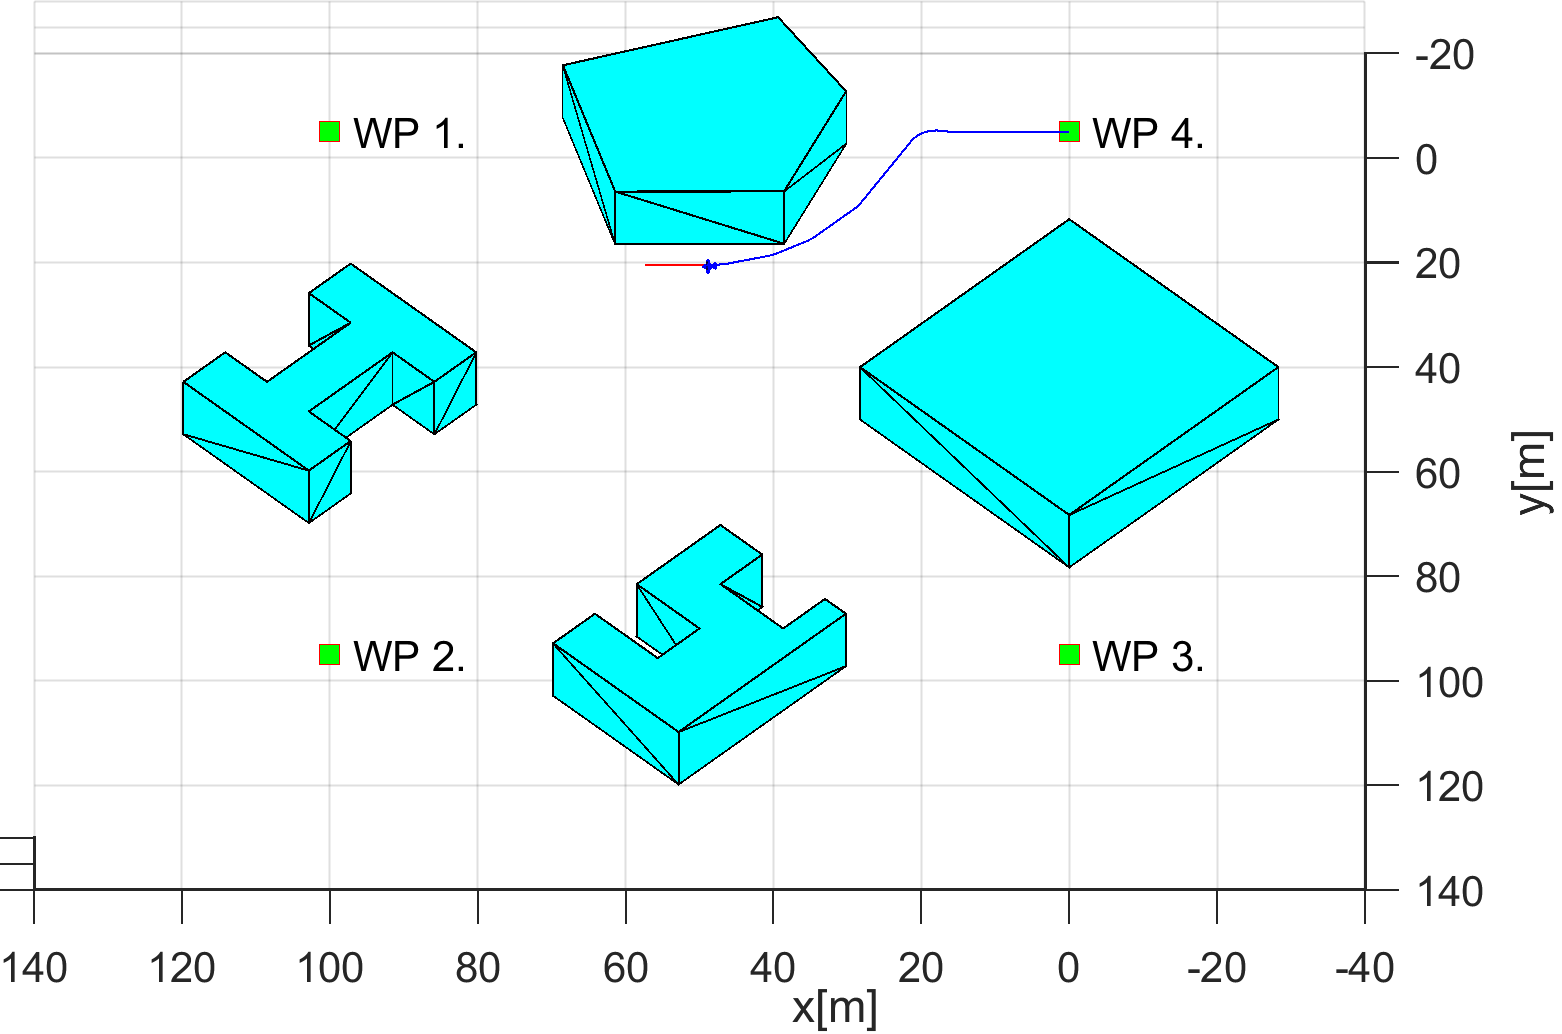
\includegraphics[width=0.9\linewidth]{\FIGDIR/NS001ConstraintsBuildingObstacle00061}
		\caption{$1^{st}$ building avoidance.}
		\label{fig:firstBuildingAvoidance}
	\end{subfigure}
	\begin{subfigure}{0.48\textwidth}
		\centering
		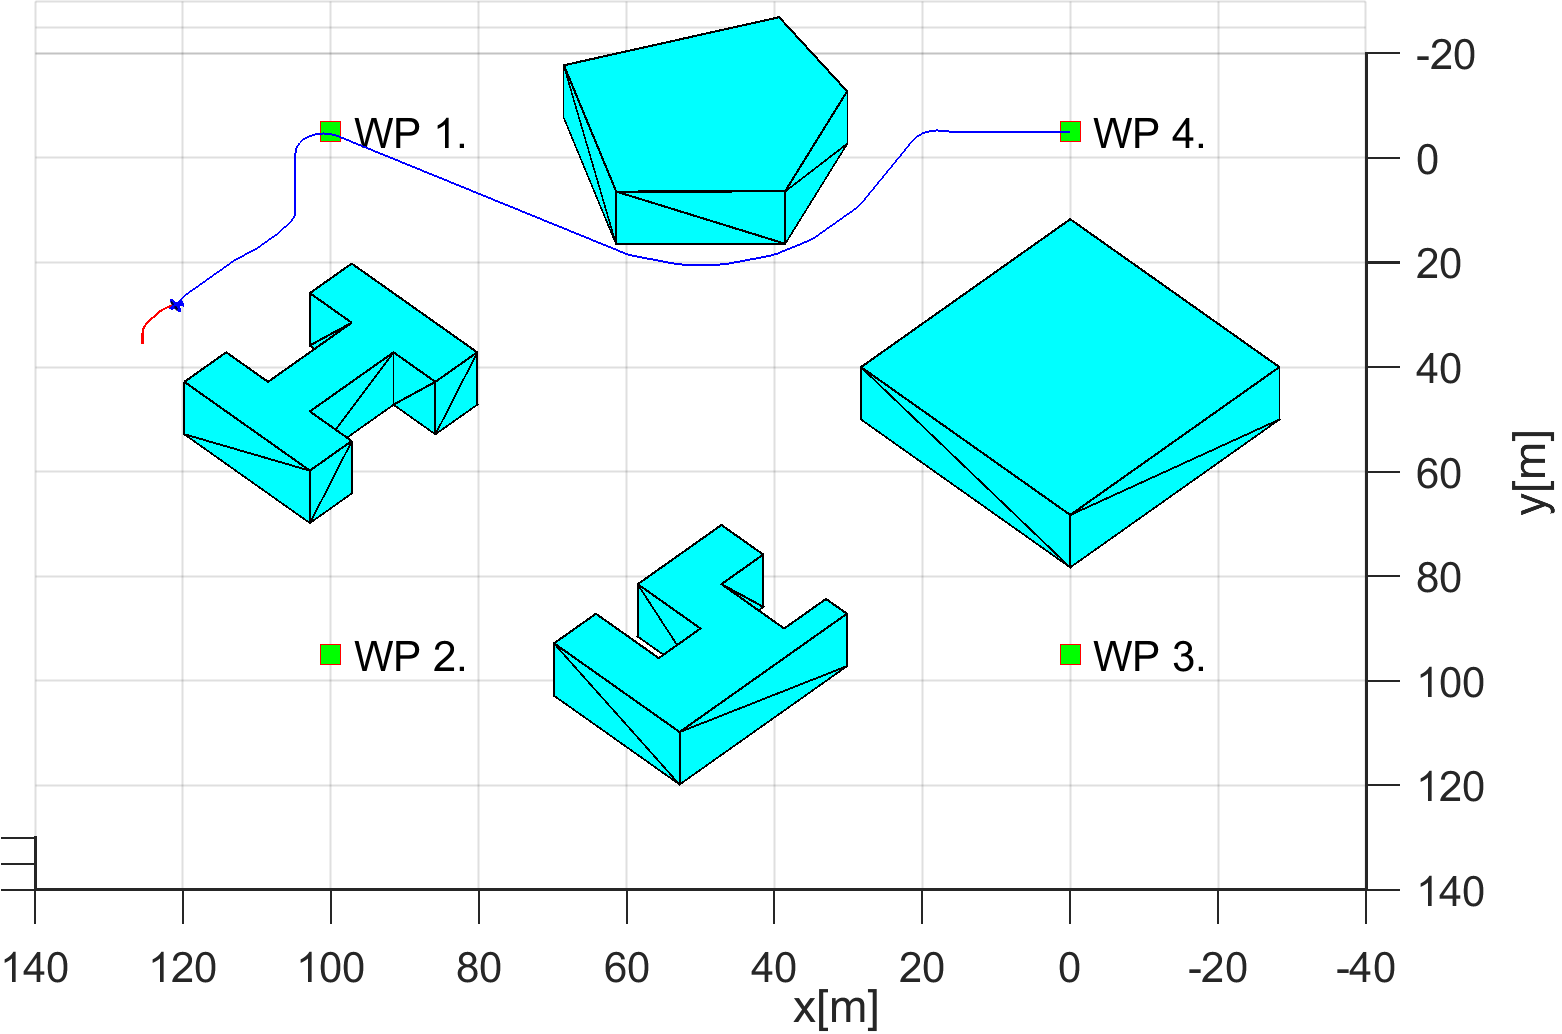
\includegraphics[width=0.9\linewidth]{\FIGDIR/NS002ConstraintsBuildingObstacles00161} 
		\caption{$1^{nd}$ building avoidance.}
		\label{fig:secondBuildingAvoidance}
	\end{subfigure}
	\\
	\begin{subfigure}{0.48\textwidth}
		\centering
		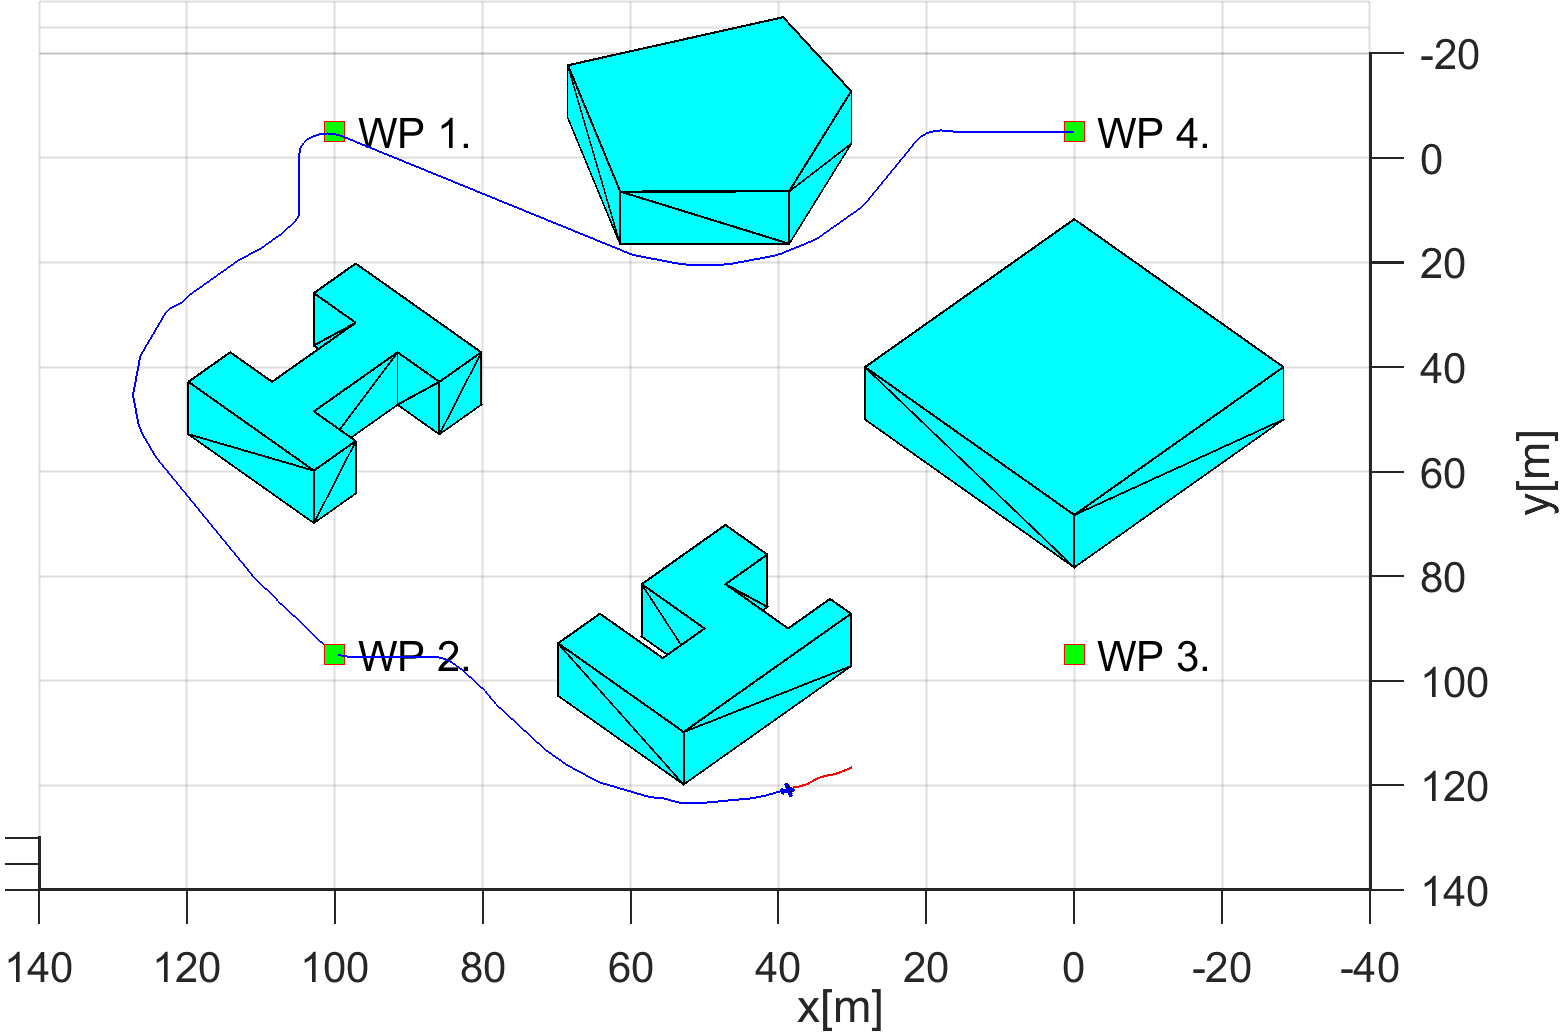
\includegraphics[width=0.9\linewidth]{\FIGDIR/NS003ConstraintsBuildingObstacles00311} 
		\caption{$3^{rd}$ building avoidance.}
		\label{fig:thirdBuidlingAvoidance}
	\end{subfigure}
	\begin{subfigure}{0.48\textwidth}
		\centering
		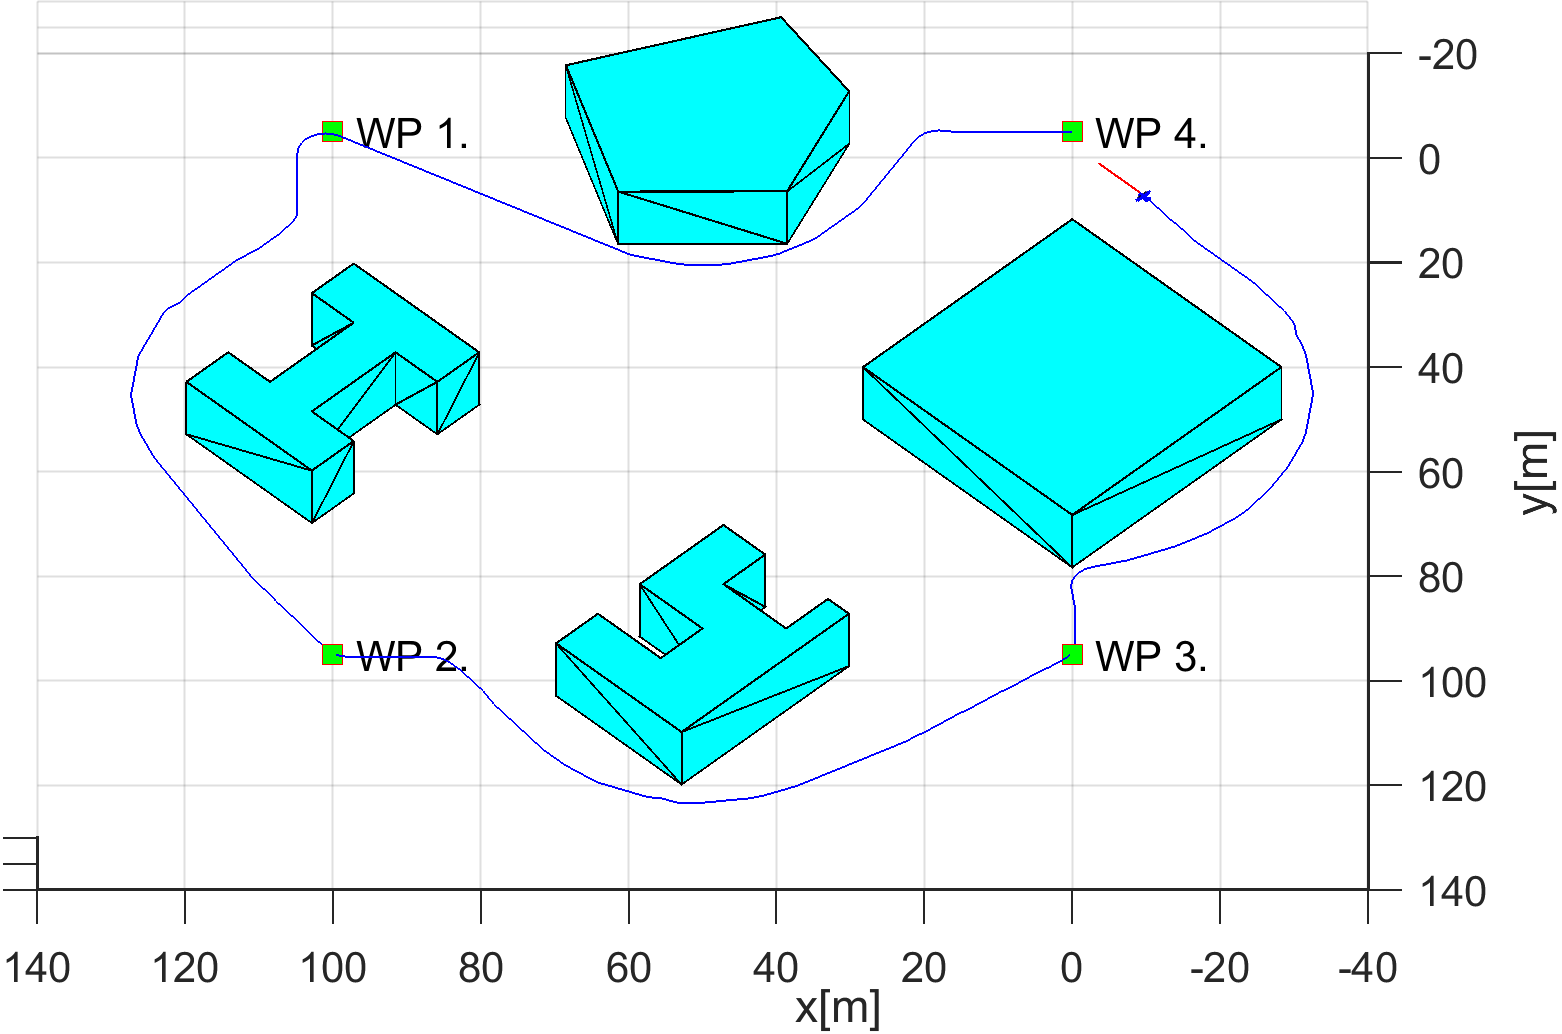
\includegraphics[width=0.9\linewidth]{\FIGDIR/NS004ConstraintsBuildingObstacles00470} 
		\caption{$4^{th}$ building avoidance.}
		\label{fig:fourthBuildingAvoidance}
	\end{subfigure}
	\caption{Test scenario for \emph{Building avoidance} (static ground obstacles). }
	\label{fig:testCaseBuildingAvoidanceSituation}
\end{figure}


\noindent\paragraph{Distance to Body/Safety Margin Evolution:} The distance of \emph{UAS} center to nearest obstacle (blue) does not broke a \emph{safety margin} (of closest obstacle (yellow)  nor \emph{body margin} of closest obstacle (red) as it can be seen in (fig. \ref{fig:testCaseBuildingAvoidancePerformance}). \emph{Acceptance condition} for \emph{algorithm mode switch} can be shown by UAS \emph{active avoidance of obstacles}.

\begin{note}
The \emph{body} and \emph{safety margins} are changing depending on \emph{UAS position and orientation}, is changing reflecting (tab. \ref{tab:obstacleSetBuildingAvoidance}) margins. 
\end{note}


\begin{figure}[H]
	\centering
	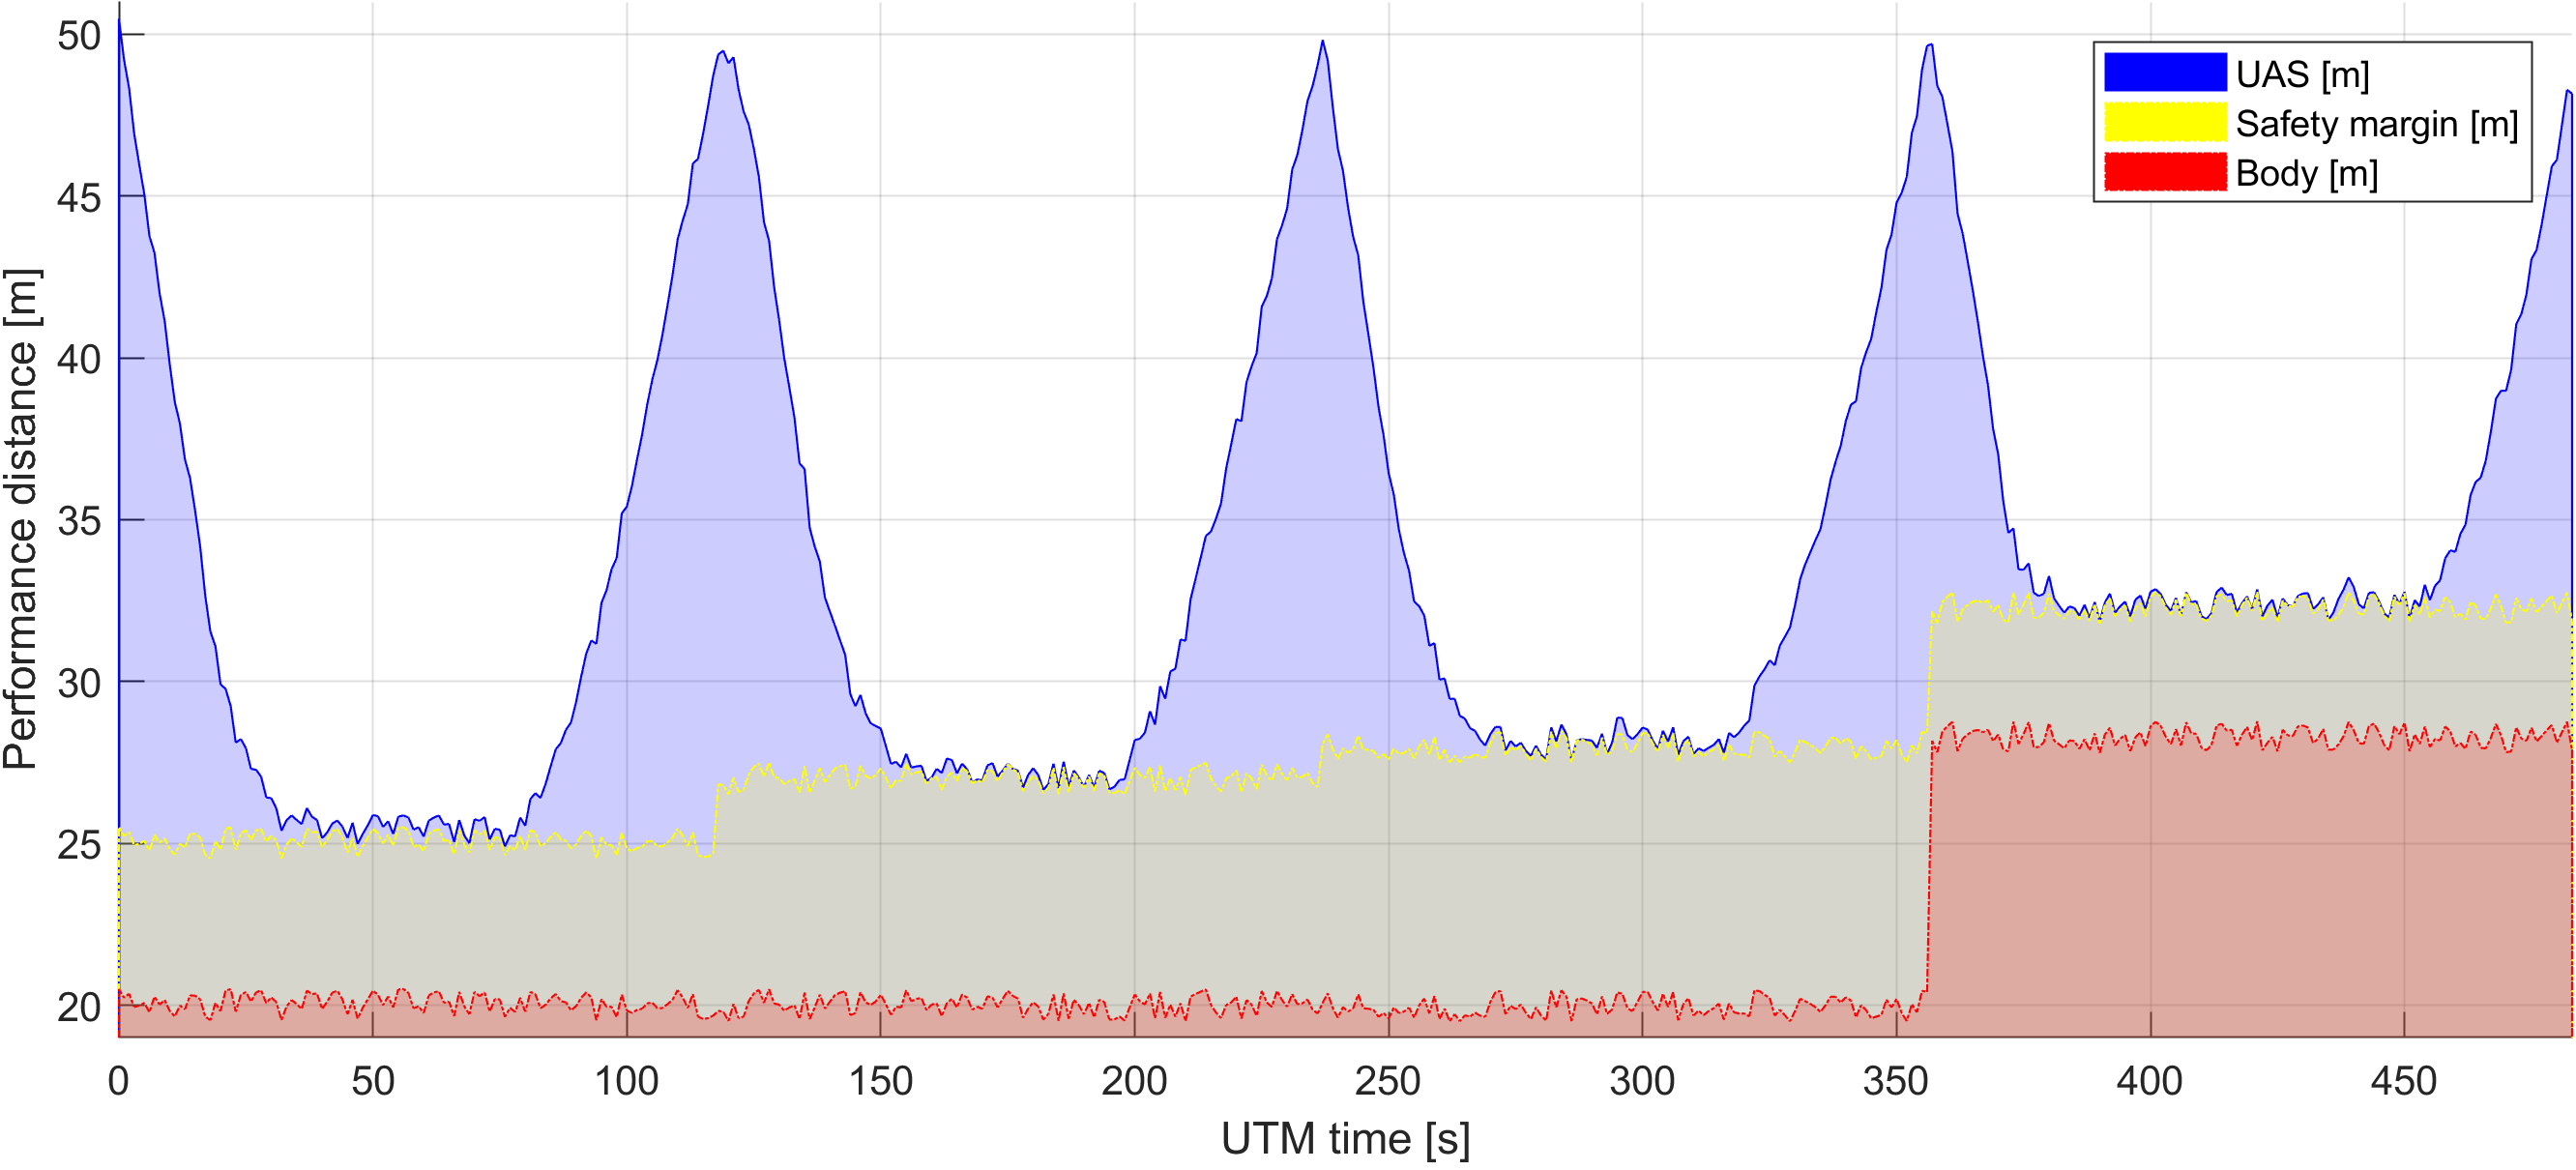
\includegraphics[width=0.8\linewidth]{\FIGDIR/NS005ConstraintsPolynomialBuildingObstaclesPerformance} 
	\caption{Distance to body/safety margin evolution for \emph{Building avoidance scenario}.}
	\label{fig:testCaseBuildingAvoidancePerformance}
\end{figure}


\noindent\paragraph{Distance to Body/Safety Margin Peaks:} Minimal distance to \emph{safety margin} is $0.69$ $m$. The \emph{minimal distance to obstacle body} is $4.69$ $m$ which is more than sufficient for tested UAS type. \emph{Safety margin acceptance criteria} have been achieved, because minimal distance is greater than zero. The minimal \emph{body margin distance} is $4.69$ $m$ for obstacle no. $4$ (tab. \ref{tab:obstacleSetBuildingAvoidance}).

\begin{table}[H]
	\centering
	\begin{tabular}{c|c||c}
	\multicolumn{2}{c||}{Parameter} & UAS 1 \\\hline\hline
	\multirow{2}{*}{Distance to Safety Margin} & min & 0.69  \\\cline{2-3}
											& max & 24.98 \\\hline
	\multirow{2}{*}{Distance to Body Margin}   & min & 4.69  \\\cline{2-3}
											& max & 29.98 
	\end{tabular}
	\caption{Distance to Body/Satety Margin Peaks for \emph{Building avoidance scenario}.}
	\label{tab:testCaseBuildingAvoidanceSafetyAndBodyMarginDistances}
\end{table}

\noindent\paragraph{Path Tracking Performance:} Reference path (green dashed line) is given as direct interconnection between waypoints (green numbered square).  The real trajectory (blue solid line) is split into its XYZ components. \emph{All mission waypoints} (fig. \ref{fig:testCaseBuildingAvoidancePathTracking}) have been reached in given order. There are some deviations on $X-Y$ horizontal axes, while the UAS was in the \emph{avoidance mode}.

\begin{figure}[H]
	\centering
	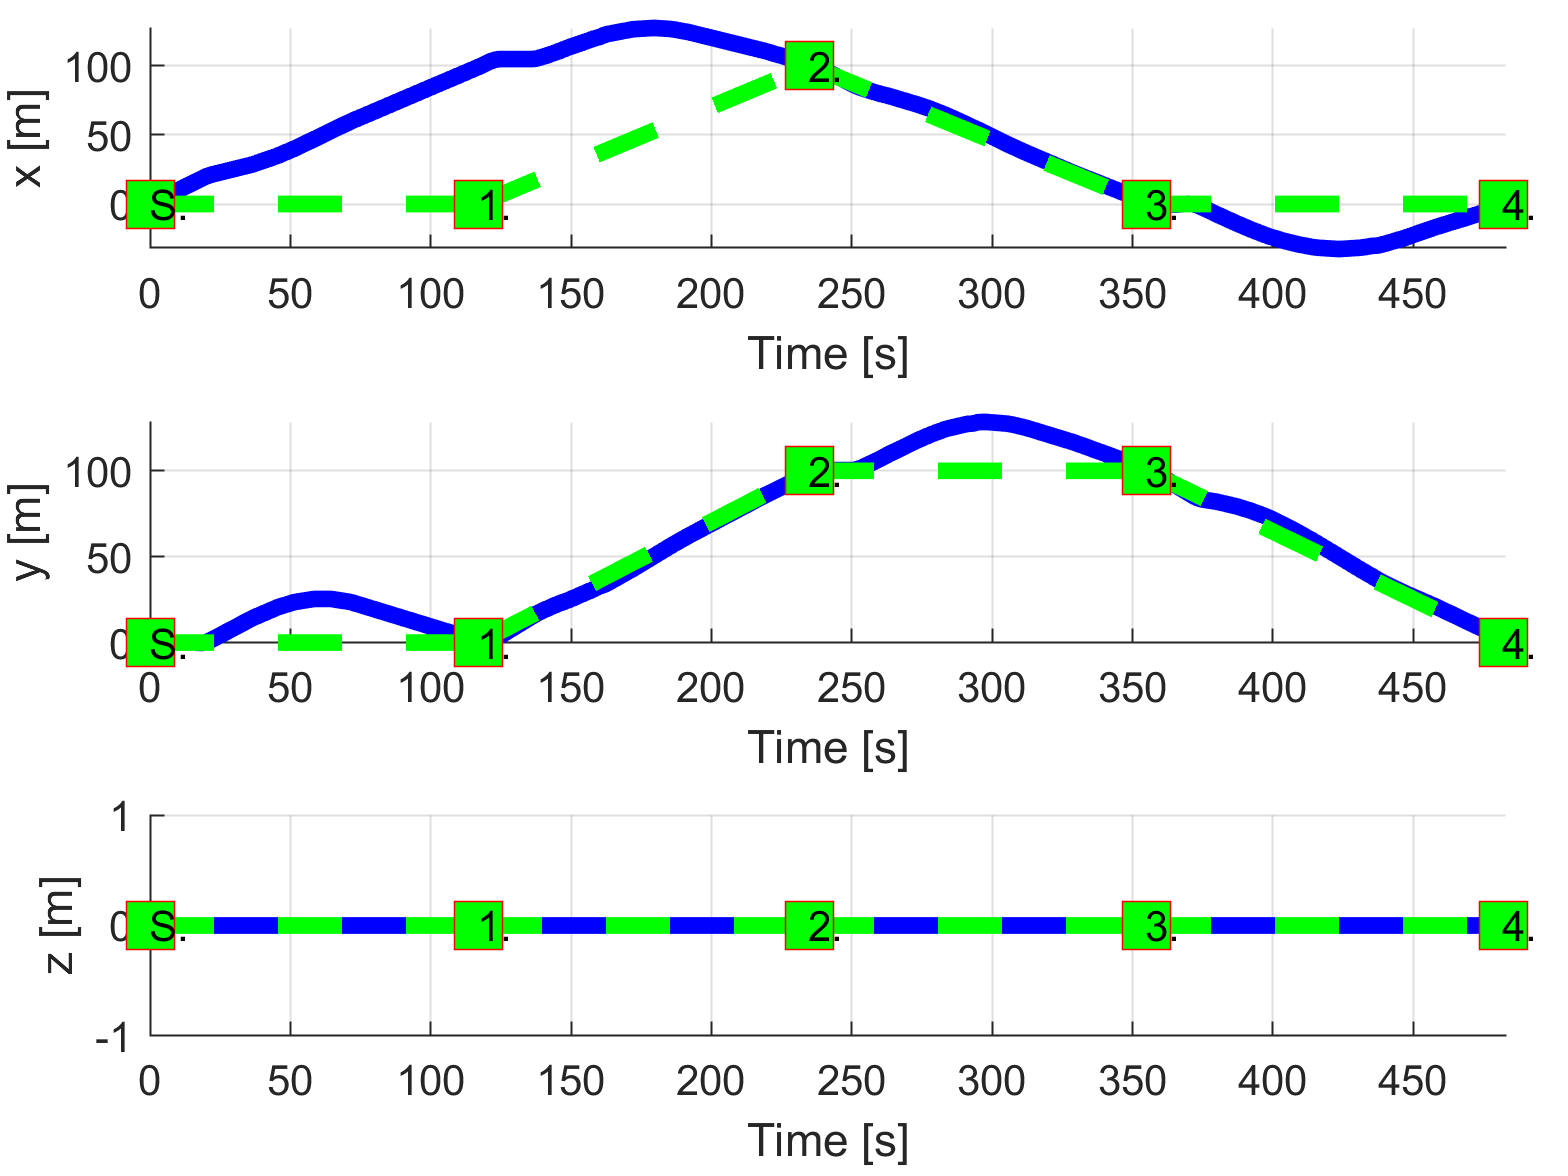
\includegraphics[width=0.55\linewidth]{\FIGDIR/NS006ConstraintsPolynomialBuildingPathFollowing} 
	\caption{\emph{Building avoidance} path tracking.}
	\label{fig:testCaseBuildingAvoidancePathTracking}
\end{figure}



\noindent\paragraph{Path Tracking Deviations:} Deviations (tab. \ref{tab:pathTrackingParametersForBuildingAvoidance}) from \emph{reference trajectory} are in expected ranges considering \emph{mission plan} (tab. \ref{tab:missionSetupForBuildingAvoidanceScenario}) and \emph{obstacle properties} (tab. \ref{tab:obstacleSetBuildingAvoidance}).
\begin{table}[H]
	\centering
	\begin{tabular}{c||c|c|c|c}
		\multirow{2}{*}{Param.} & \multicolumn{4}{c}{UAS 1} \\\cline{2-5}
						& $\mathscr{WP}_1$  & $\mathscr{WP_2}$  & $\mathscr{WP}_3$  & $\mathscr{WP}_4$  \\\hline\hline
		  $\max |x|$    & 104      & 86      & 5.34       & 32.52 \\\hline
		  $\max |y|$    & 25.39      & 6.59       & 28.2      & 4.55 \\\hline
		  $\max |z|$    & 0      & 0      &   0    & 0 \\\hline
		  $\max dist.$  & 107.05       & 86.2      & 28.7       & 32.84 \\
	\end{tabular}
	\caption{Path tracking for properties \emph{Building avoidance}.}
	\label{tab:pathTrackingParametersForBuildingAvoidance}
\end{table}

% 01-Building Avoidance Scenario:
\paragraph{Computation Load:} The \emph{computation load} for \emph{scenario} (fig.\ref{fig:buildingAvoidanceComputationTime}) shows used time (y-axis) over decision frame (x-axis).

There is slight increase in \emph{computation time} when UAS is in \emph{Emergency Avoidance Mode}.

\begin{figure}[H]
    \centering
    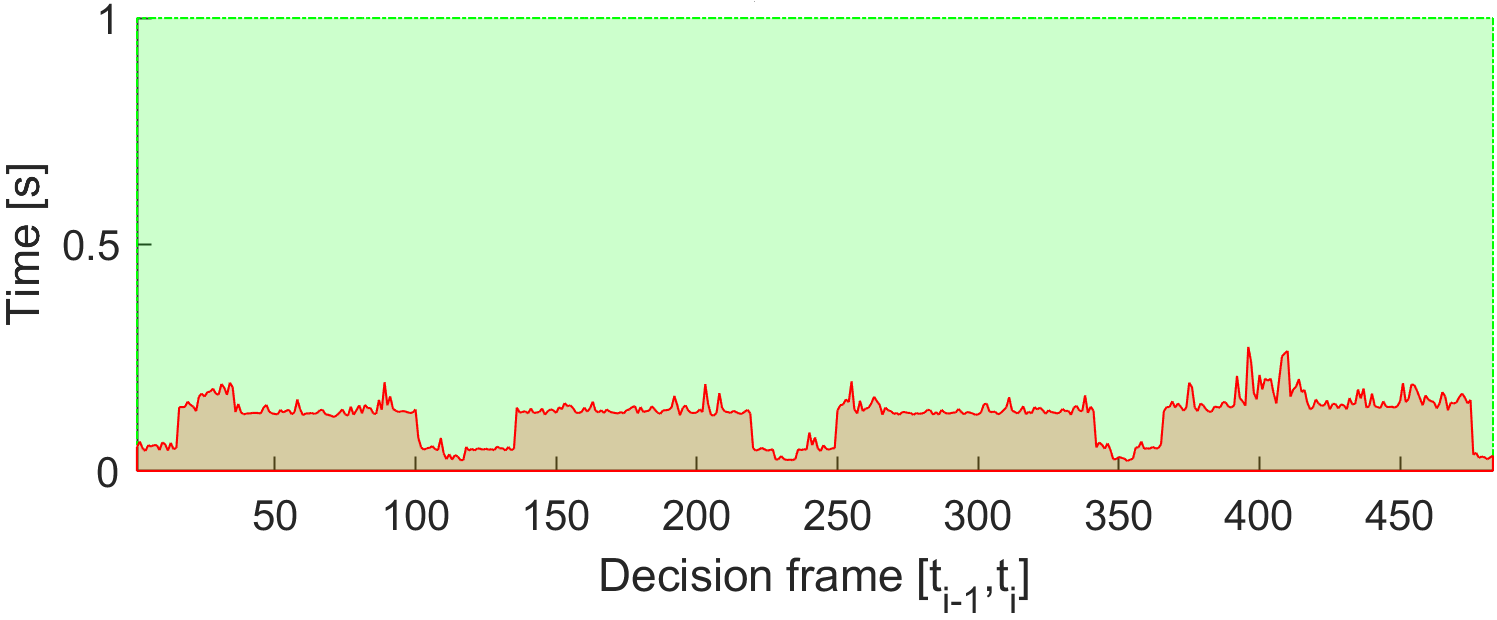
\includegraphics[width=0.65\linewidth]{\FIGDIR/NS092BuildingAvoidanceComputationTime} 
    \caption{Computation time for \emph{Building avoidance} scenario.}
    \label{fig:buildingAvoidanceComputationTime}
\end{figure}
  



    	\subsection{Slalom}\label{s:testSlalom}

\paragraph{Scenario:} The \emph{UAS} is flying the mission given by (tab. \ref{tab:missionSetupSlalomScenario}) in the \emph{open-space environment}. A Operational space is more clustered than in case of \emph{Building Avoidance} (sec. \ref{s:testBuildingAvoidance}). There map of notable \emph{buildings} with defined \emph{safety and body margins} imposing additional flight constraints. The \emph{UAS} is flying through partially known space with some charted obstacles. 

The \emph{goal waypoint} is hidden behind the sensors line of sight. There is multiple cost equivalent trajectories to reach the goal. 

\begin{table}[H]
    \centering
    \begin{tabular}{c|c||c}
        \multicolumn{2}{c||}{Position} & \multirow{2}{*}{$\mathscr{WP}_1$} \\\cline{1-2}
        $[x,y,z]$           & $[\theta,\varpi,\psi]$           & \\\hline\hline
        $[25,5,0]^T $        & $[0^\circ,0^\circ,90^\circ]^T$    & $[35,75,0]^T$        \\ 
    \end{tabular}
    \caption{Mission setup for \emph{Slalom} scenario.}
    \label{tab:missionSetupSlalomScenario}
\end{table}

\paragraph{Obstacle set:} Obstacles are discovered during a flight by \emph{UAS LiDAR Sensor}. The set of obstacles is defined in (tab. \ref{tab:obstacleSetSlalom}) Some obstacles does not have \emph{Line of Sight} during a flight, which causes additional constraints during \emph{avoidance trajectory selection} process.

\begin{table}[H]
    \centering
    \begin{tabular}{c|c|c|c|c|c}
        \multicolumn{2}{c|}{Obstacle} & \multicolumn{3}{c|}{Body Margin} & \multirow{2}{*}{Safety Margin}\\\cline{1-5}
        position & type & min. & max. & avg. &   \\\hline\hline
        multiple (4) & hospital & $[0.5,1]$ & $[2.2,3.1]$ & $[1.5,3]$  & $[1,3]$ \\\hline 
        multiple (7) & unusual  & $[0.3,1]$ & $[2.3,3.5$] & $[2,3]$  & $[1,4]$ \\\hline
        multiple (3) & square   & $[3,4]$   & $[4,5]$     & $[4,5]$ & $[1,4]$   \\
     \end{tabular}
    \caption{\emph{Obstacle set} for \emph{Slalom} scenario.}
    \label{tab:obstacleSetSlalom}
\end{table}

\paragraph{Main goal:} Show \emph{static obstacle avoidance} in \emph{clustered environment} with \emph{shorter decision frames} due the obstacle density. Show \emph{hidden waypoint navigation capability} and Behind Line of Sight impact on decision making. 

\paragraph{Acceptance Criteria} are given as follow: 
\begin{enumerate}
    \item \emph{Hidden waypoint reach} - the UAS will safely reach \emph{goal waypoint}.
    \item \emph{Minimal safety margin distance} $\ge$ 0.
    \item \emph{Hindered space} is accounted into decision making (BLOS impact).
\end{enumerate}

\paragraph{Testing setup:}  The \emph{standard test setup} defined in (tab.  \ref{tab:testMovementOrientations}. \ref{tab:testUASBasicParameters}. \ref{tab:testNavigationGridBasic}. \ref{tab:testAvoidanceGridBasic}. \ref{tab:testUASColoring}) is used with following parameter override:

\begin{enumerate}
    \item \emph{Avoidance grid - type} - \emph{ACAS-like} with enabled \emph{Horizontal maneuvers}
\end{enumerate}

\begin{note}
The \emph{vertical separation} was disabled, because \emph{UAS} will just increase its altitude to reach \emph{goal waypoint}.
\end{note}

\paragraph{Simulation run:} Notable moments from this \emph{simulation run} (fig. \ref{fig:testCaseSlalomwithHiddenWaypoint}) are following:

\begin{enumerate}
    \item \emph{Open space obstacle} (fig. \ref{fig:slalomOpenSpaceObstacle}) - avoidance of open space obstacle, while tracking \emph{hidden waypoint}. This is standard navigation procedure, the middle building in front of \emph{goal waypoint} is hidden by building in front of UAS.
        
    \item \emph{Hidden waypoint navigation} is shown in three stages start (fig. \ref{fig:slalomHiddenWaypointStart}), middle (fig. \ref{fig:slalomHiddenWaypointMiddle}), and end phase (fig. \ref{fig:slalomHiddenWaypointEnd}).The \emph{hidden goal waypoint} has been reached and first acceptance criteria was fullfilled.  The \emph{Decision points} of navigational loop are placed in very high density around this area. The avoided building had following traps which were avoided:
    
    \begin{enumerate}[a.]
        \item Trap (fig. \ref{fig:slalomHiddenWaypointStart}) on the left side of \emph{UAS} was avoided, because there was no turning point inside of space.
    
        \item Trap (fig. \ref{fig:slalomHiddenWaypointMiddle}) on the left side of UAS was avoided, because it was not wide enough to be considered as trajectory space.
    \end{enumerate}
\end{enumerate}


\begin{figure}[H]
    \centering
    \begin{subfigure}{0.48\textwidth}
    	\centering
        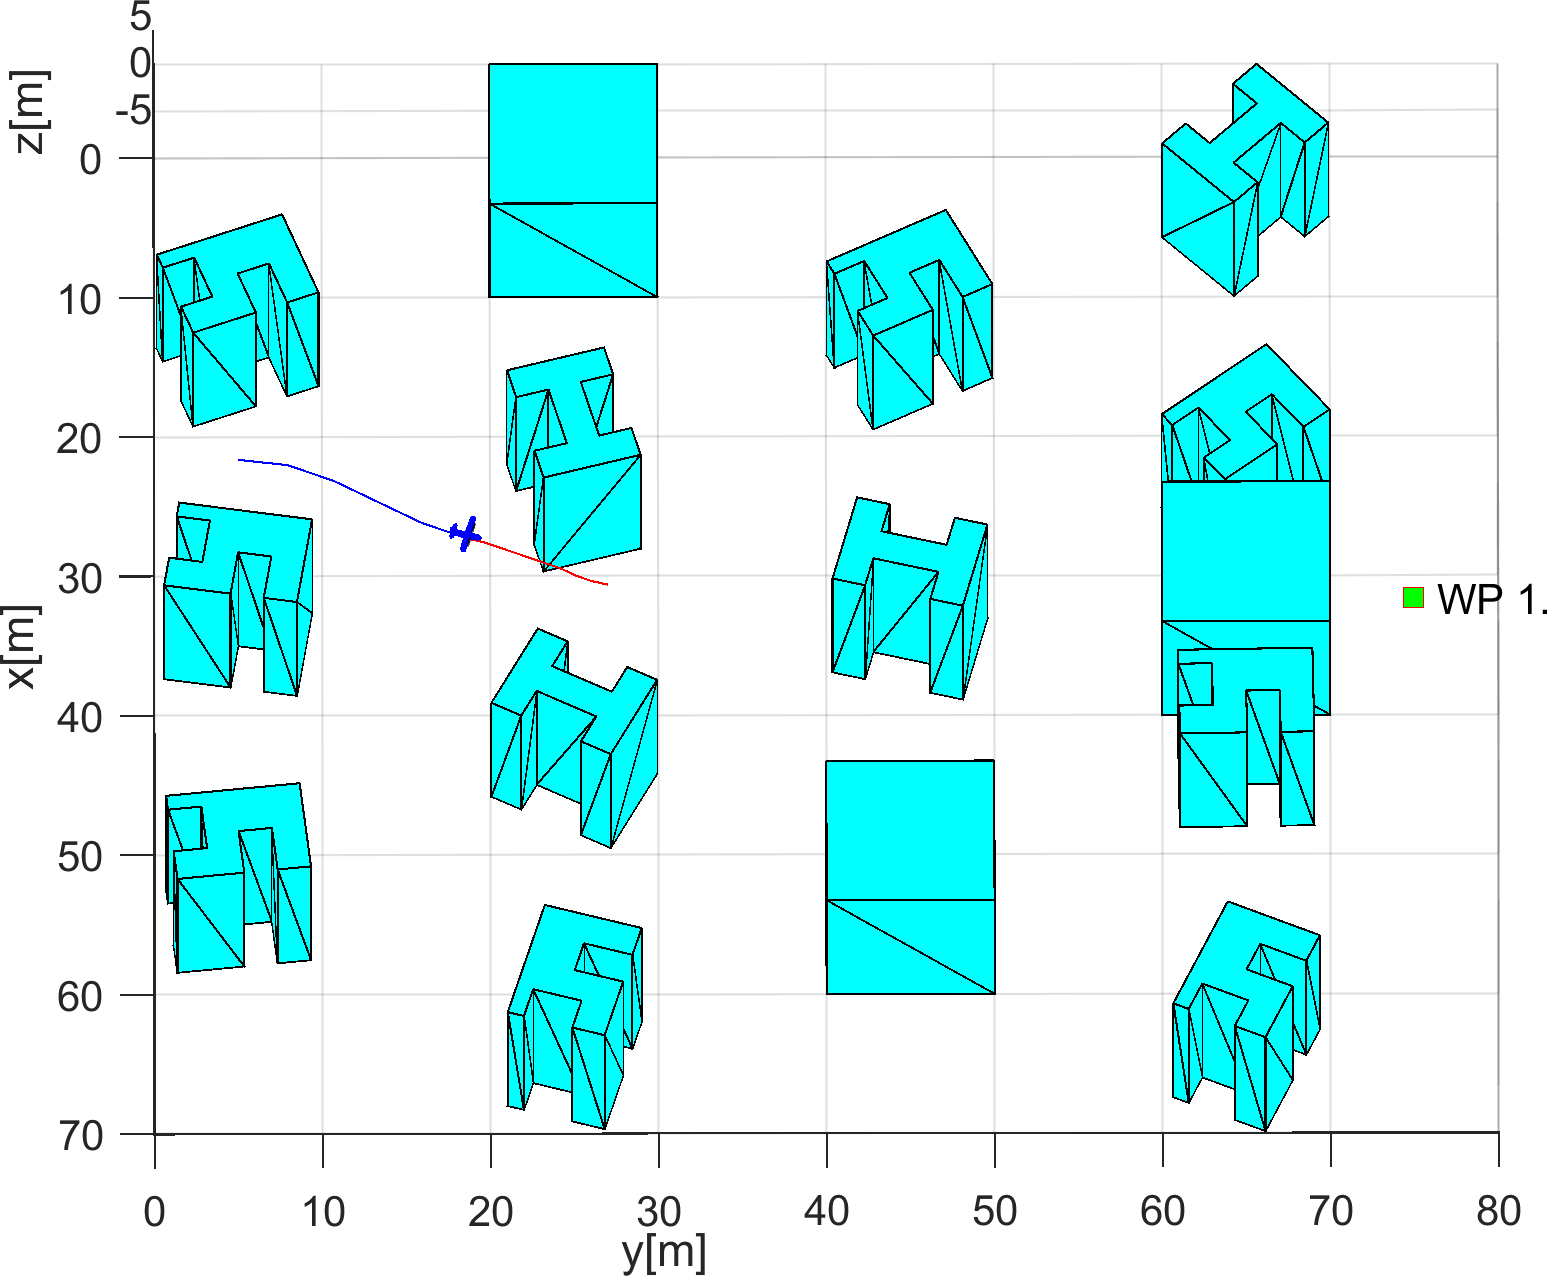
\includegraphics[width=0.9\linewidth]{\FIGDIR/NS007ConstraintsPolynomialSlalom-00015}
        \caption{Open space obstacle.}
        \label{fig:slalomOpenSpaceObstacle}
    \end{subfigure}
    \begin{subfigure}{0.48\textwidth}
    	\centering
        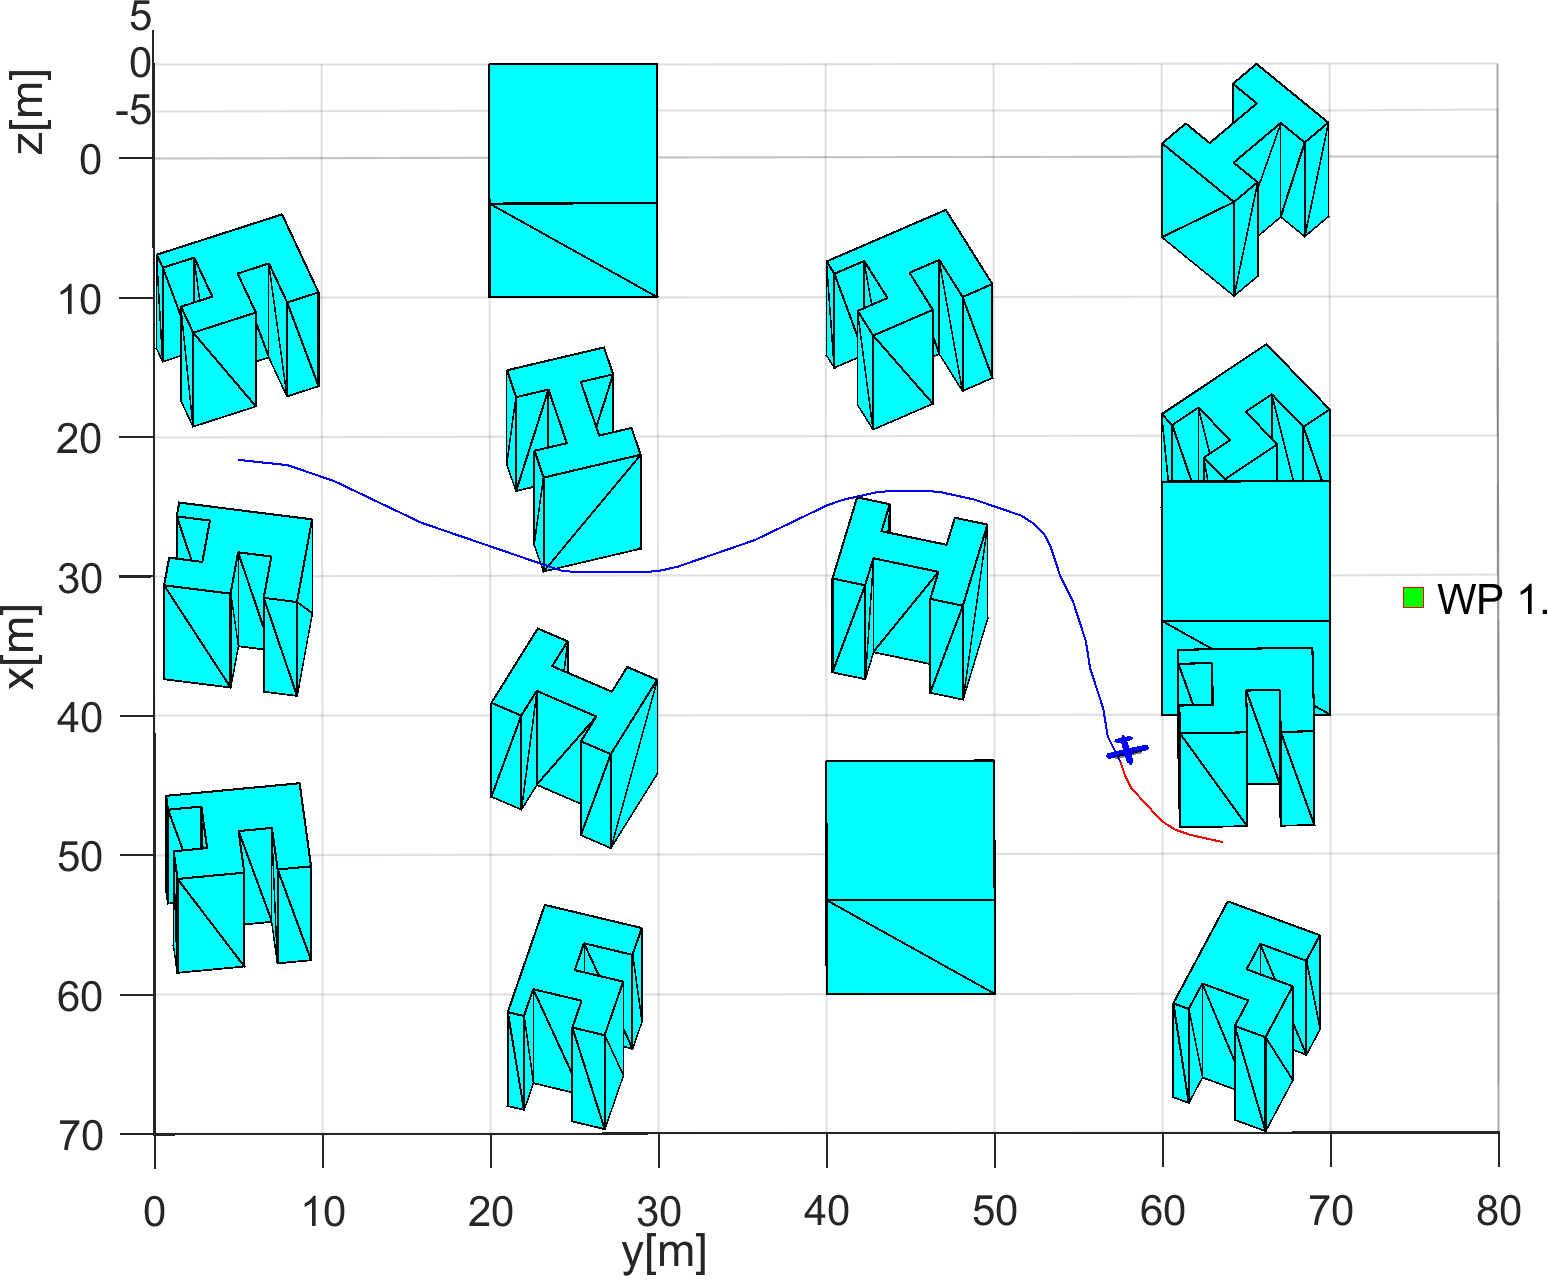
\includegraphics[width=0.9\linewidth]{\FIGDIR/NS008ConstraintsPolynomialSlalom-00069} 
        \caption{Hidden waypoint start.}
        \label{fig:slalomHiddenWaypointStart}
    \end{subfigure}
    \\
    \begin{subfigure}{0.48\textwidth}
	    \centering
        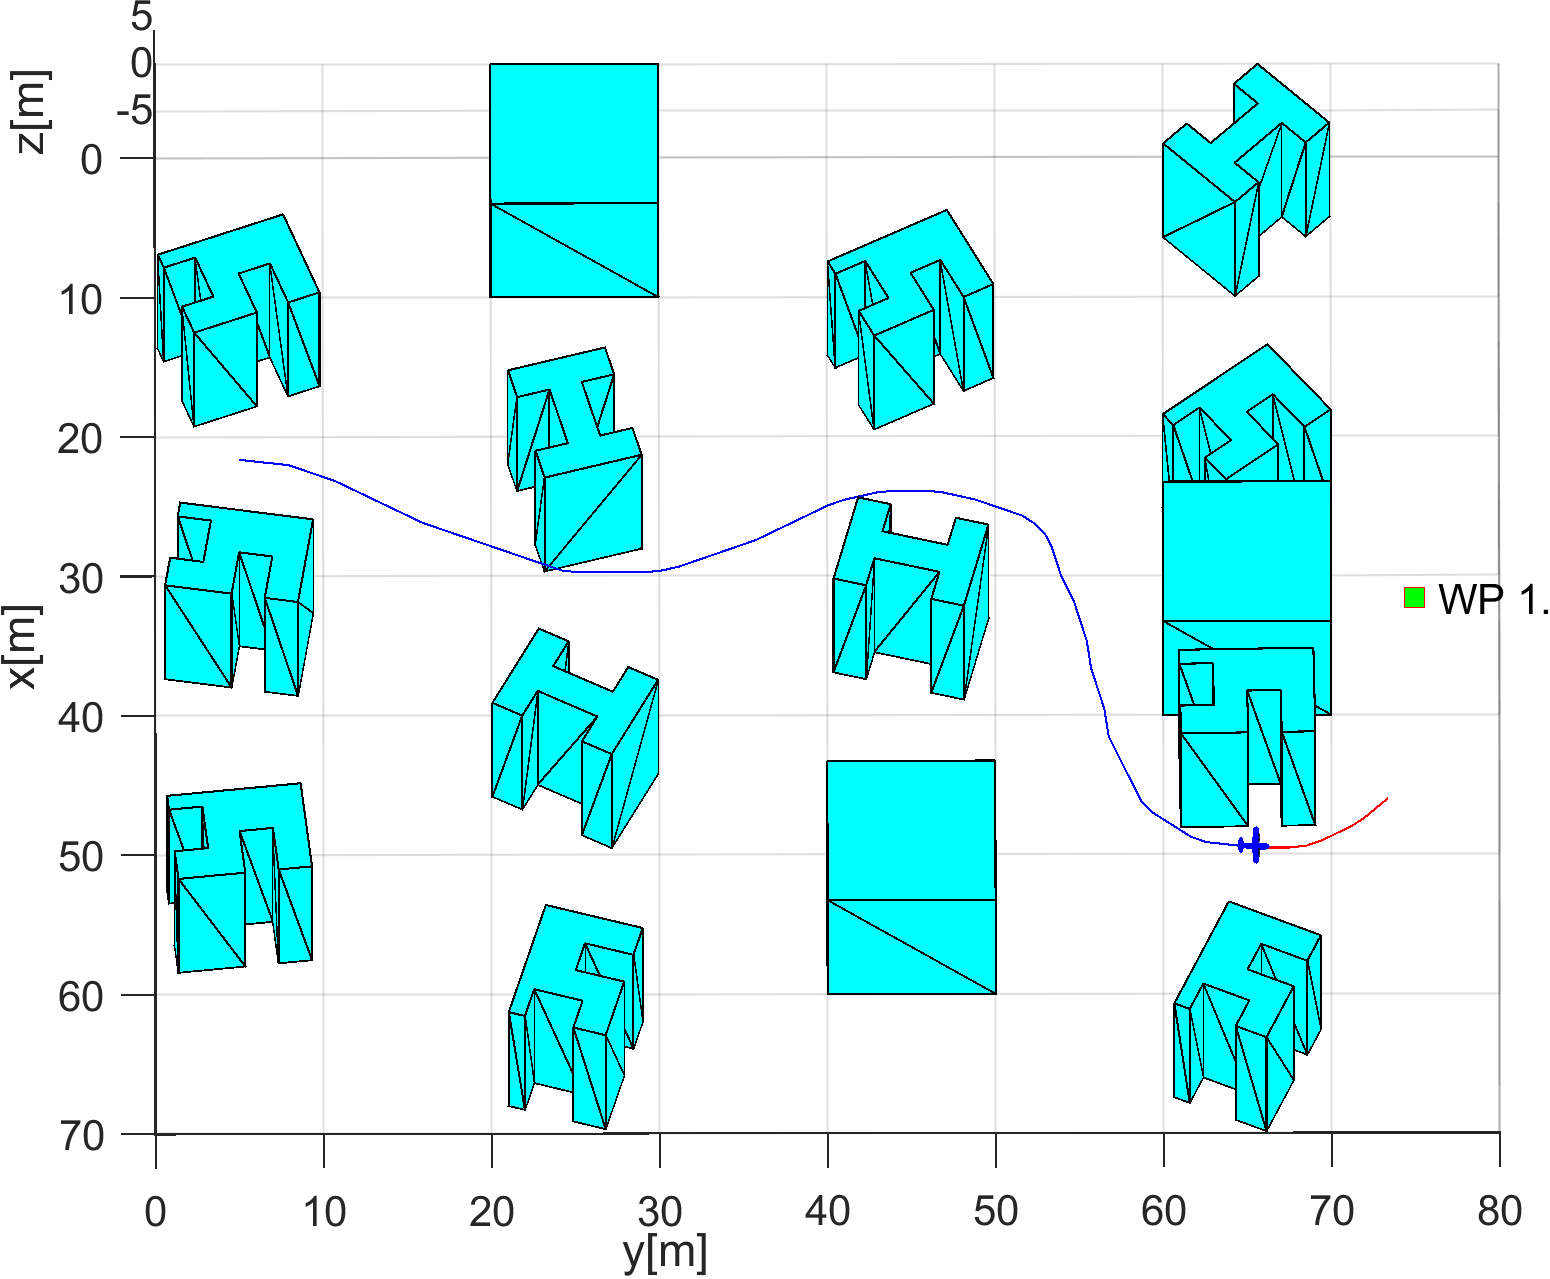
\includegraphics[width=0.9\linewidth]{\FIGDIR/NS009ConstraintsPolynomialSlalom00080} 
        \caption{Hidden waypoint middle.}
        \label{fig:slalomHiddenWaypointMiddle}
    \end{subfigure}
    \begin{subfigure}{0.48\textwidth}
    	\centering
        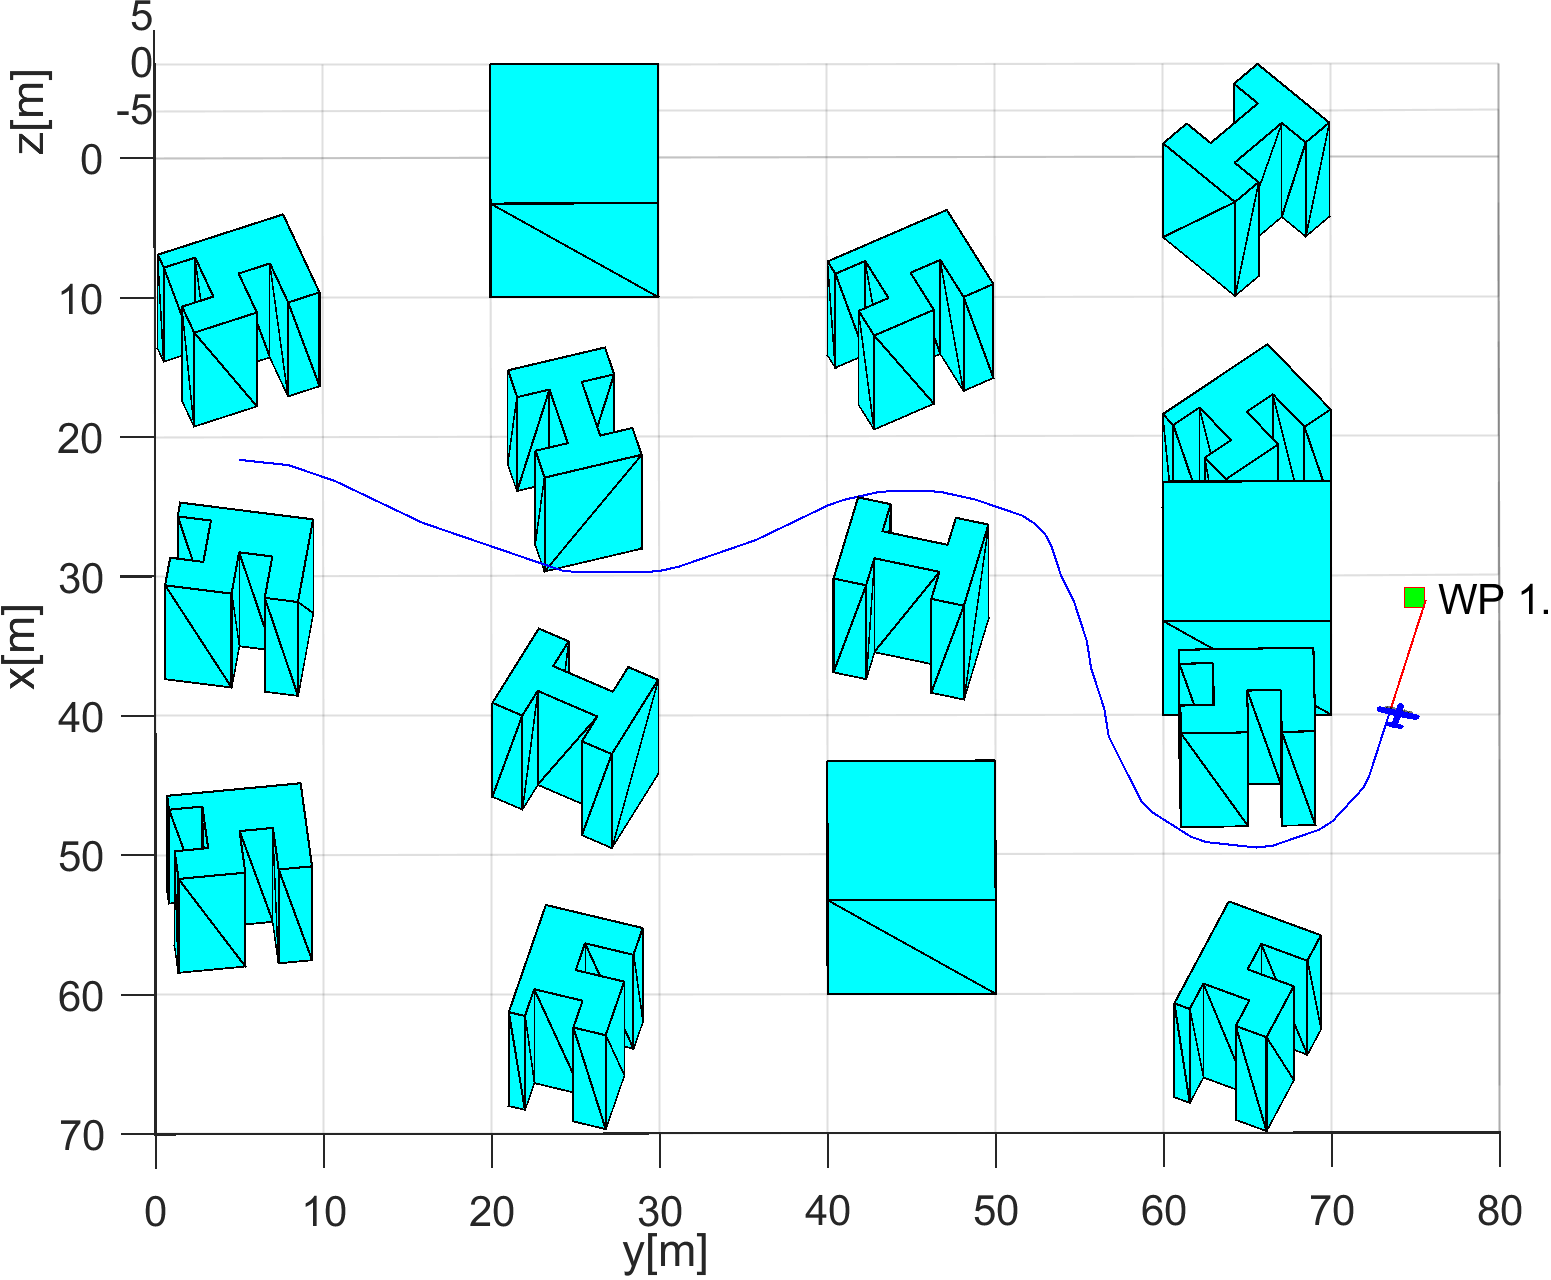
\includegraphics[width=0.9\linewidth]{\FIGDIR/NS010ConstraintsPolynomialSlalom00094} 
        \caption{Hidden waypoint end.}
        \label{fig:slalomHiddenWaypointEnd}
    \end{subfigure}
    \caption{Test scenario for \emph{Slalom} with \emph{hidden waypoint}. }
    \label{fig:testCaseSlalomwithHiddenWaypoint}
\end{figure}


\paragraph{Distance to Safety Margin Evolution:} The \emph{UAS} (blue fill) does not break a \emph{safety margin} (yellow fill) nor \emph{body margin} (red fill) as you can seen in (fig. \ref{fig:testCaseSlalomAvoidancePerformance}). Hindered space is accounted into decision making, because the distance to closest obstacle will never breach \emph{safety margin} (yellow fill). If it was not, the UAS will break \emph{safety} or \emph{body} margin. 

\emph{Body} and \emph{Safety margin} are changing values depending on the \emph{nearest obstacle} and \emph{mutual position of obstacle and UAS}. The ranges of \emph{body} and \emph{safety margins} are reflected in (tab. \ref{tab:obstacleSetSlalom}). 

\begin{figure}[H]
    \centering
    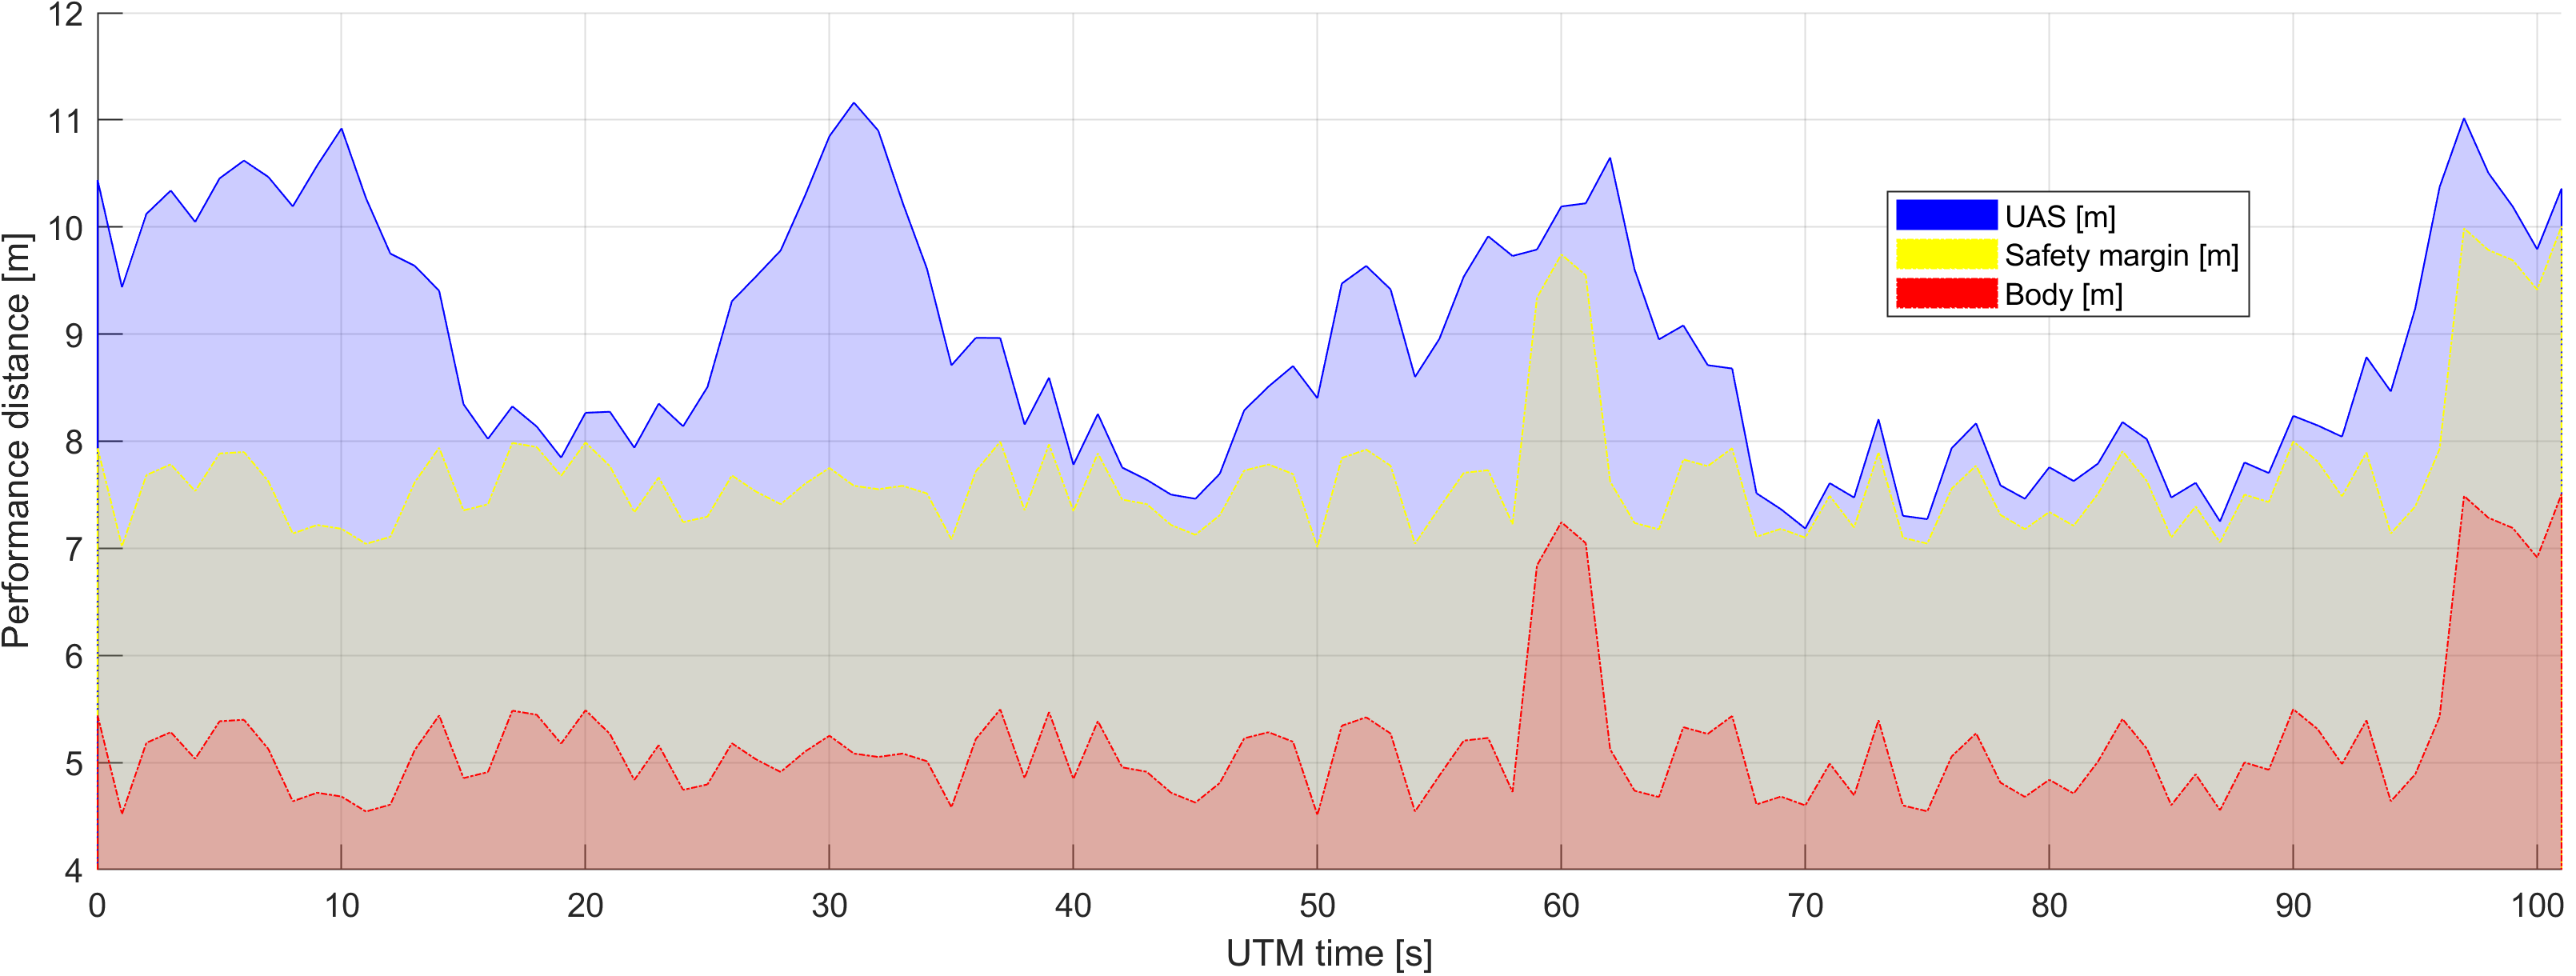
\includegraphics[width=0.8\linewidth]{\FIGDIR/NS011ConstraintsPolynomialSlalomPerformance} 
    \caption{Distance to Safety Margin Evolution for \emph{Slalom scenario}.}
    \label{fig:testCaseSlalomAvoidancePerformance}
\end{figure}

\paragraph{Distance to Safety Margin Peaks:} The boundary of \emph{safety} and  \emph{body} margin is given in (tab. \ref{tab:testCaseSlalomSafetyAndBodyMarginDistances}). The minimal distance of \emph{UAS border}(blue line) to \emph{safety margin boundary} (yellow line fig. \ref{fig:testCaseSlalomAvoidancePerformance}) is $0.0856$ $m$ which can be considered as marginal $0$. The minimal \emph{body margin} distance is $2.5856$ $m$ which is reflects \emph{safety margin} $2.5$ $m$ at that moment. The condition $safety Margin Distance \ge 0$ holds.
    
    
The difference between minimal and maximal \emph{safety margin distance} is $\sim 3$ $m$ which indicates that mission environment is  tightly packed with obstacles.

\begin{table}[H]
    \centering
    \begin{tabular}{c|c||c}
    \multicolumn{2}{c||}{Parameter} & UAS 1 \\\hline\hline
    \multirow{2}{*}{safety margin distance} & min & 0.0856\\\cline{2-3}
                                            & max & 3.7391 \\\hline
    \multirow{2}{*}{body margin distance}   & min & 2.5856  \\\cline{2-3}
                                            & max & 6.2391 
    \end{tabular}
    \caption{\emph{Slalom} safety and body margin distances.}
    \label{tab:testCaseSlalomSafetyAndBodyMarginDistances}
\end{table}


\paragraph{Path tracking performance:} Path tracking is given in (fig. \ref{fig:testCaseSlalomPathTracking}). The line between Starting position (green square, marked S) and  goal waypoint (green square marked 1) is reference trajectory (green dashed line). The flown trajectory (blue solid line) is showing evolution over mission time (Time [s]) in global coordinate frame split into three axes (x[m], y[m], z[m]). The UAS was all time in \emph{Emergency Avoidance Mode} due the vicinity of dangerous obstacles. 

The \emph{UAS} reached final navigation waypoint, which fulfills acceptance criteria. The UAS has taken a significant detour (x[m] evolution) due to hidden \emph{waypoint}. 

The test has been run multiple times to check if \emph{Right-Up} preference for avoidance is always selected. \emph{Small noise} (0.5-1m) was added to obstacle positions. The algorithm always chose similar deterministic path. The higher noise levels were not possible due the obstacle original size (tab. \ref{tab:obstacleSetSlalom}).

\begin{figure}[H]
    \centering
    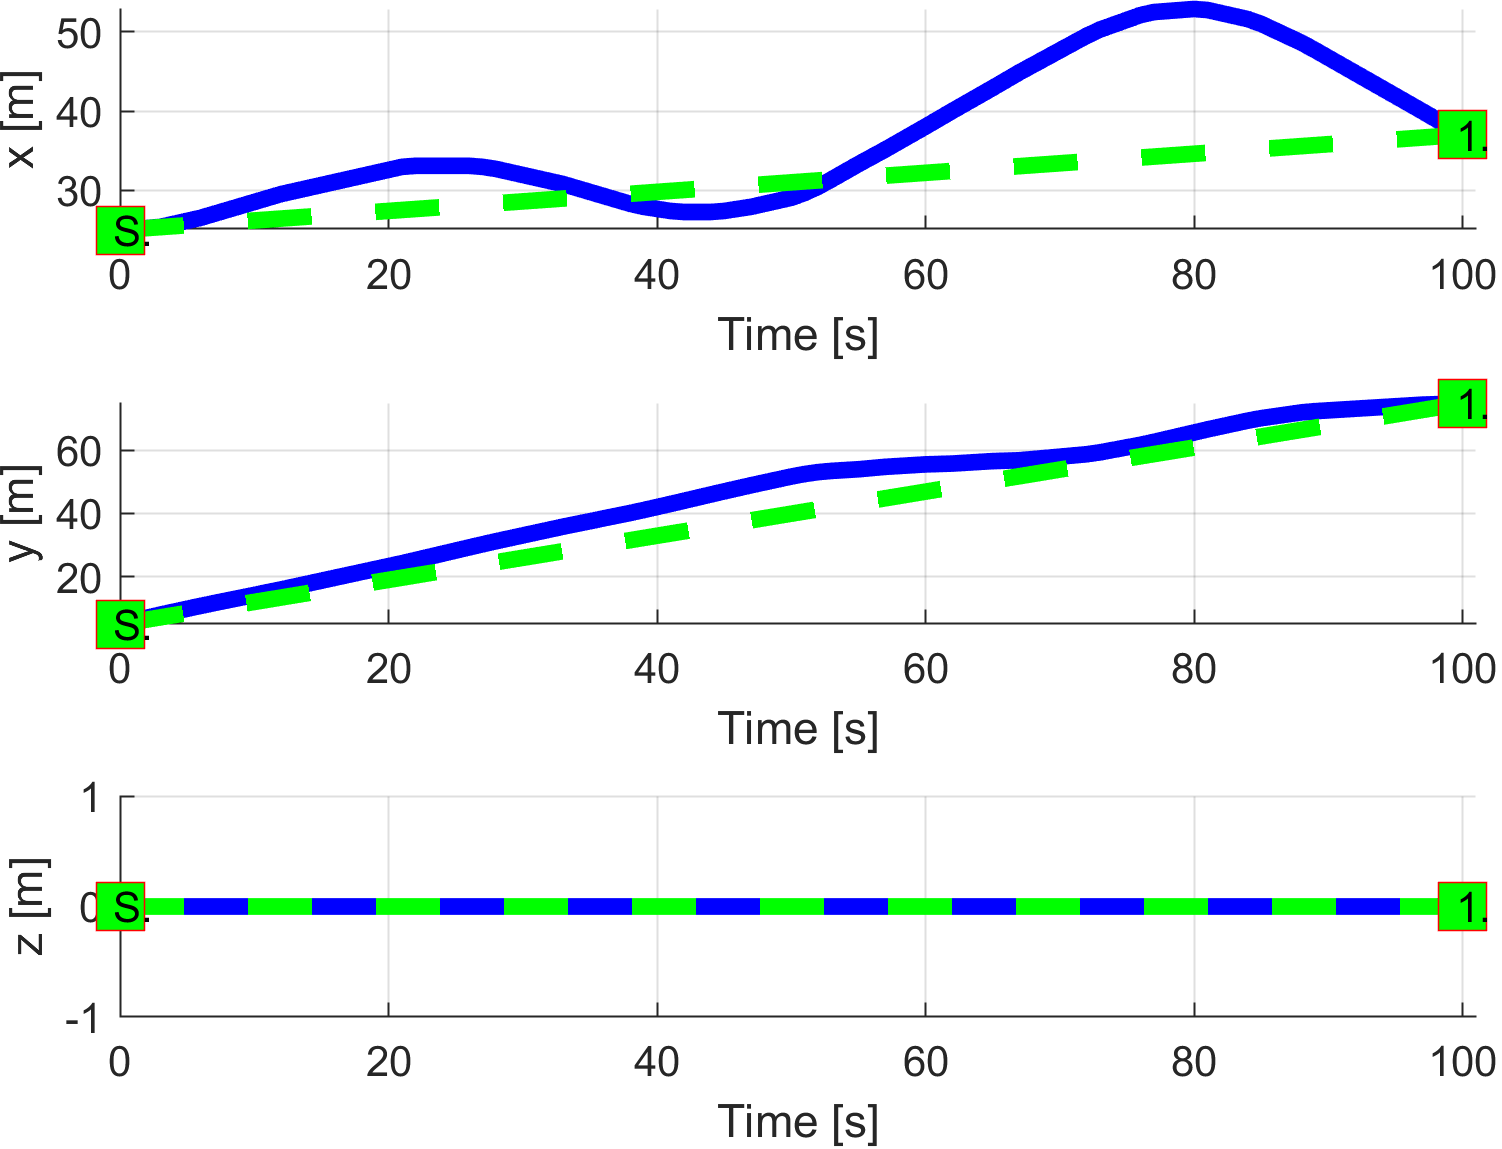
\includegraphics[width=0.55\linewidth]{\FIGDIR/NS012ConstraintsPolynomialSlalomPathFollowing} 
    \caption{\emph{Slalom} path tracking.}
    \label{fig:testCaseSlalomPathTracking}
\end{figure}


\paragraph{Path Tracking Deviations:} Deviations given in (tab. \ref{tab:pathTrackingParametersForSlalomAvoidance}) from \emph{reference trajectory} (fig. \ref{fig:testCaseSlalomPathTracking}) are in expected ranges considering \emph{mission plan} (tab. \ref{tab:missionSetupSlalomScenario}) and \emph{obstacle properties} (\ref{tab:obstacleSetSlalom}).

\begin{table}[H]
    \centering
    \begin{tabular}{c||c}
        \multirow{2}{*}{Param.} & UAS 1\\\cline{2-2}
                        & $\mathscr{WP}_1$  \\\hline\hline
          $\max |x|$    & 17.90      \\\hline
          $\max |y|$    & 12.41    \\\hline
          $\max |z|$    & 0        \\\hline
          $\max dist.$  & 20.06   \\
    \end{tabular}
    \caption{Path tracking properties for \emph{Slalom} scenario.}
    \label{tab:pathTrackingParametersForSlalomAvoidance}
\end{table}





    	\subsection{Maze}\label{s:testMaze}

\paragraph{Scenario:} The UAS is flying a mission given by (tab. \ref{tab:missionSetupMazeScenario}) in \emph{closed space} constrained by ground from bottom, airspace constraint from top and building from sides. The maneuverable space is \emph{maze-like} with  \emph{hidden goal waypoint}.

There exists a \emph{Obstacle map} with defined \emph{safety} and \emph{body margins}. \emph{Reference trajectories} (direct interconnection of initial position and \emph{goal waypoint}) is going trough \emph{partially known space} with some charted obstacles.

\begin{table}[H]
    \centering
    \begin{tabular}{c|c||c}
        \multicolumn{2}{c||}{Position} & \multirow{2}{*}{$\mathscr{WP}_1$} \\\cline{1-2}
        $[x,y,z]$           & $[\theta,\varpi,\psi]$           & \\\hline\hline
        $[15,15,0]^T $        & $[0^\circ,0^\circ,0^\circ]^T$    & $[15,75,0]^T$        \\ 
    \end{tabular}
    \caption{Mission setup for \emph{Maze} scenario.}
    \label{tab:missionSetupMazeScenario}
\end{table}

\paragraph{Obstacle set:} \emph{Obstacles} are discovered during a flight by \emph{UAS LiDAR} sensor. The \emph{Obstacle set} is defined in (tab. \ref{tab:obstacleSetMaze}). the obstacles are placed in \emph{virtual grid} with \emph{cell size} $10 \times 10 m$. There are following obstacles:

\begin{enumerate}
    \item $5\times$  \emph{Hospital building} - H-shaped, with two open traps, with minimal body margin in range $0.5 - 1m$, with maximal body margin in range $2.2 - 3.1 m$ and variable \emph{safety margin} in range $1-3 m$.
    
    \item $12\times$ \emph{Unusual trap building} - square shaped building with two traps on neighbouring side, with minimal body margin in range $0.3 - 1m$, with maximal body margin in range $2.3 - 3.5 m$ and variable \emph{safety margin} in range $1-4 m$.
    
    \item $6\times$  \emph{Square building} - square shaped building with minimal body margin in range $3-4 m$, with maximal body margin in range $4-5 m$ and variable \emph{safety margin} in range $1-4m$.
    
    \item $7\times$  \emph{U-shaped Trap} - thin walled U shaped trap designed to catch incoming flying objects, with minimal body margin in range $2-4m$, maximal body margin in range $3-5 m$ and various \emph{safety margin} in range $1-2 m$.
\end{enumerate}

The purpose of these \emph{Obstacles} except \emph{Square building} type is to create false positive path diversions. These diversions are designed to take \emph{UAS} into unsolvable situation. \emph{Avoidance} of traps is possible due \emph{Reach set properties}, because many scenarios for avoidance can be evaluated at once.

\begin{table}[H]
    \centering
    \begin{tabular}{c|c|c|c|c|c}
        \multicolumn{2}{c|}{Obstacle} & \multicolumn{3}{c|}{Body Margin} & \multirow{2}{*}{Safety Margin}\\\cline{1-5}
        position & type & min. & max. & avg. &   \\\hline\hline
        multiple (5) & hospital & $[0.5,1]$ & $[2.2,3.1]$ & $[1.5,3]$  & $[1,3]$ \\\hline 
        multiple (12) & unusual  & $[0.3,1]$ & $[2.3,3.5$] & $[2,3]$    & $[1,4]$ \\\hline
        multiple (6) & square   & $[3,4]$   & $[4,5]$     & $[4,5]$    & $[1,4]$ \\\hline
        multiple (7) & trap     & $[2,4]$   & $[3,5]$     & $[2,4]$    & $[1,2]$ \\
     \end{tabular}
    \caption{\emph{Obstacle set} for \emph{Maze} scenario.}
    \label{tab:obstacleSetMaze}
\end{table}

\paragraph{Main Goal:} Demonstrate static obstacle avoidance in closed space navigation. Focus on determinism of \emph{avoidance run}. Demonstrate the possibilities of primitives \emph{right-hand} maze solver incorporated into \emph{Navigation-loop}.

\paragraph{Acceptance Criteria:}
\begin{enumerate}
    \item \emph{Do not break top/bottom boundaries} - the \emph{UAS} Z coordinate should not leave range $-5$ to $5 m$. The boundary break occurs when there is no feasible horizontal path and UAS needs to climb up to resolve situation.
    
    \item{Minimal safety margin distance} $\ge$ $0m$.
    
    \item\emph{Reach hidden goal waypoint} by solving simple maze (tab. \ref{tab:missionSetupMazeScenario}).
\end{enumerate}

\paragraph{Testing Setup:} The \emph{standard test setup} defined in (tab.  \ref{tab:testMovementOrientations}, \ref{tab:testUASBasicParameters}, \ref{tab:testNavigationGridBasic}, \ref{tab:testAvoidanceGridBasic}, \ref{tab:testUASColoring}) is used with following parameter override:

\begin{enumerate}
    \item \emph{Avoidance grid - type} - \emph{ACAS-like} with enabled \emph{Horizontal maneuvers}
\end{enumerate}

\paragraph{Simulation Run:} Notable moments from  the simulation run (fig. \ref{fig:testCaseMazeSolver}) are following:

\begin{enumerate}
    \item \emph{The Maze} consist from heavy constrained turns: $1^{st}$ turn (fig. \ref{fig:mazeFirstTurn}), $2^{nd}$ turn (fig. \ref{fig:mazeSecondTurn}), and $3^{rd}$ turn (fig. \ref{fig:mazeThirdTurn}). The hidden waypoint reach is given by (fig. \ref{fig:mazeWaypointReach}).
        
    \item UAS is constantly in \emph{Emergency Avoidance mode}, because there is always a presence of obstacle,
        
    \item \emph{Navigation path} is located in slim corridor with width only 3-6 meters. Mutual distance of obstacles is 20 meters and combined margins takes 14-17 meters.
        
    \item \emph{Maze scenario} was very close to urban environment in terms of obstacle density and computation complexity.
        
    \item \emph{Avoidance run} computation complexity scaled linearly with count of active obstacles in Field of View.
    
    \item \emph{Hidden Goal Waypoint} have been reached as shown in (fig. \ref{fig:mazeWaypointReach}). This satisfy \emph{reach hidden waypoint} acceptance criterion. 
\end{enumerate}


\begin{figure}[H]
    \centering
    \begin{subfigure}{0.48\textwidth}
    	\centering
        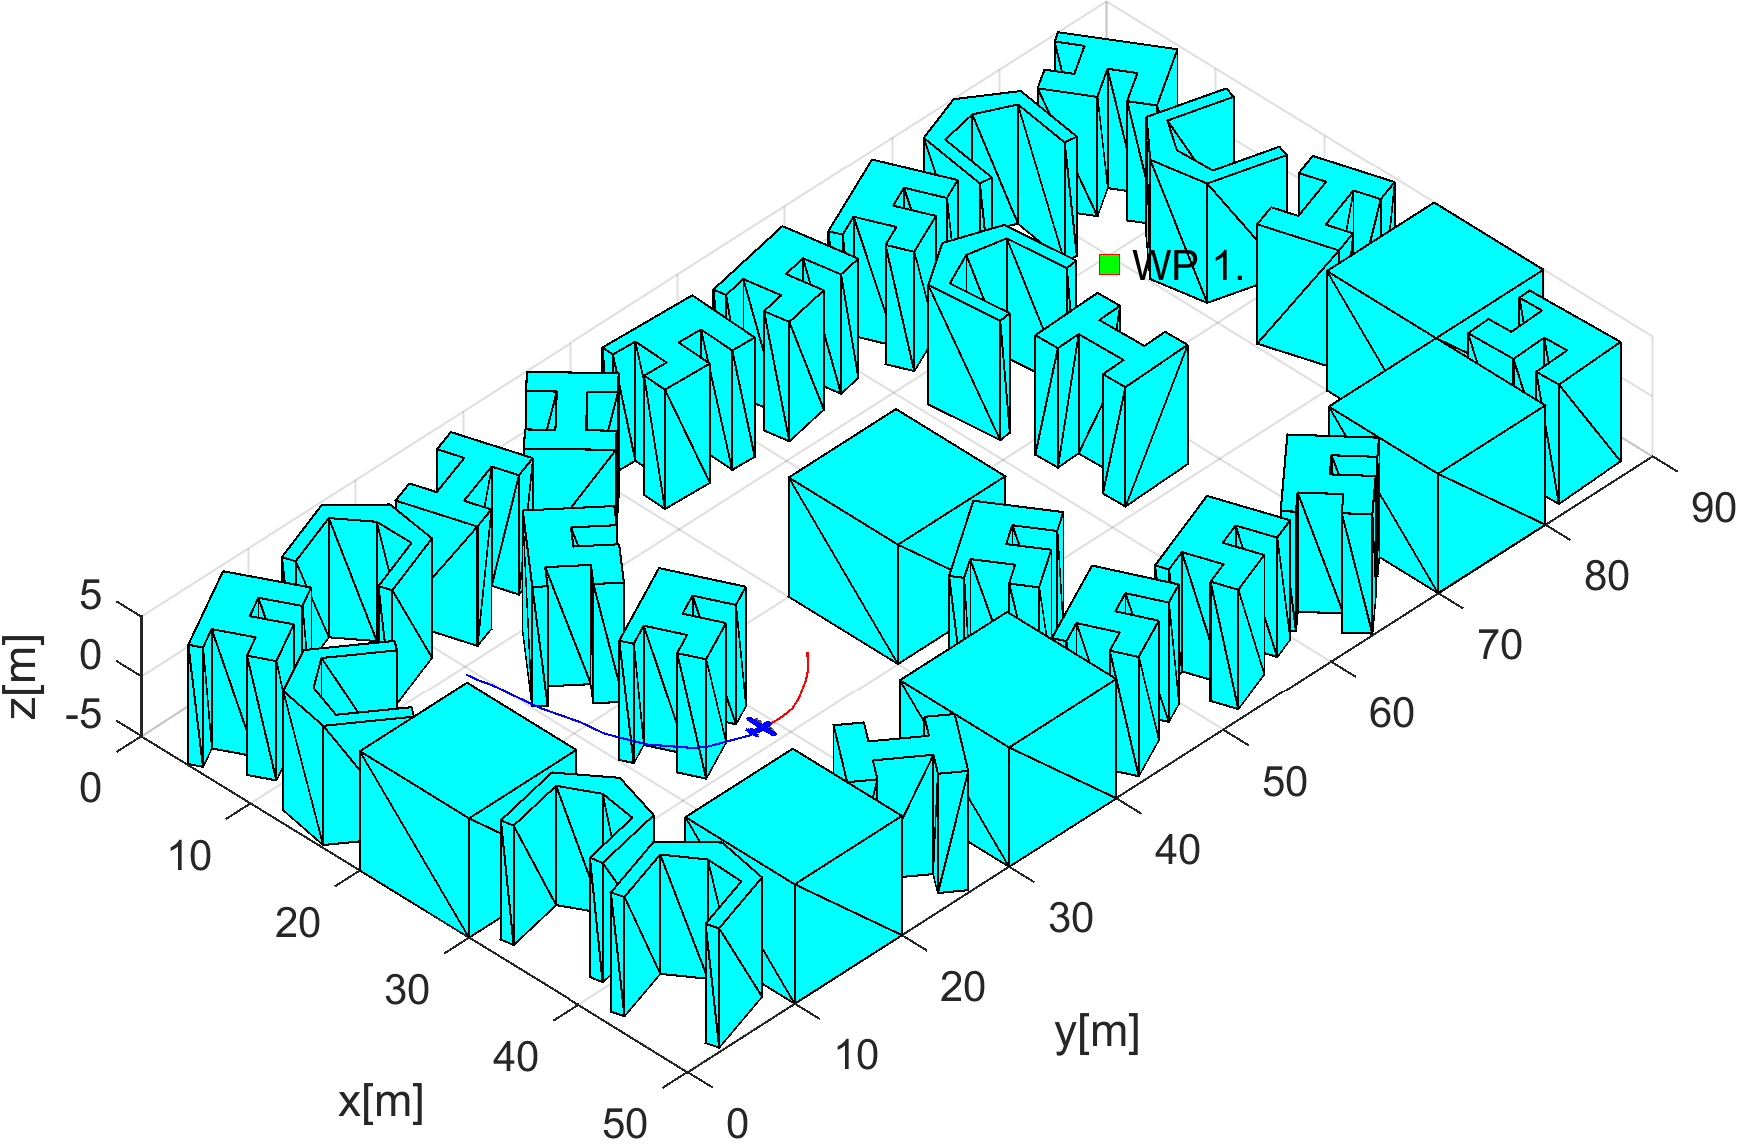
\includegraphics[width=0.9\linewidth]{\FIGDIR/NS013ConstraintsPolynomialMaze00022}
        \caption{$1^{st}$ turn.}
        \label{fig:mazeFirstTurn}
    \end{subfigure}
    \begin{subfigure}{0.48\textwidth}
	    \centering
        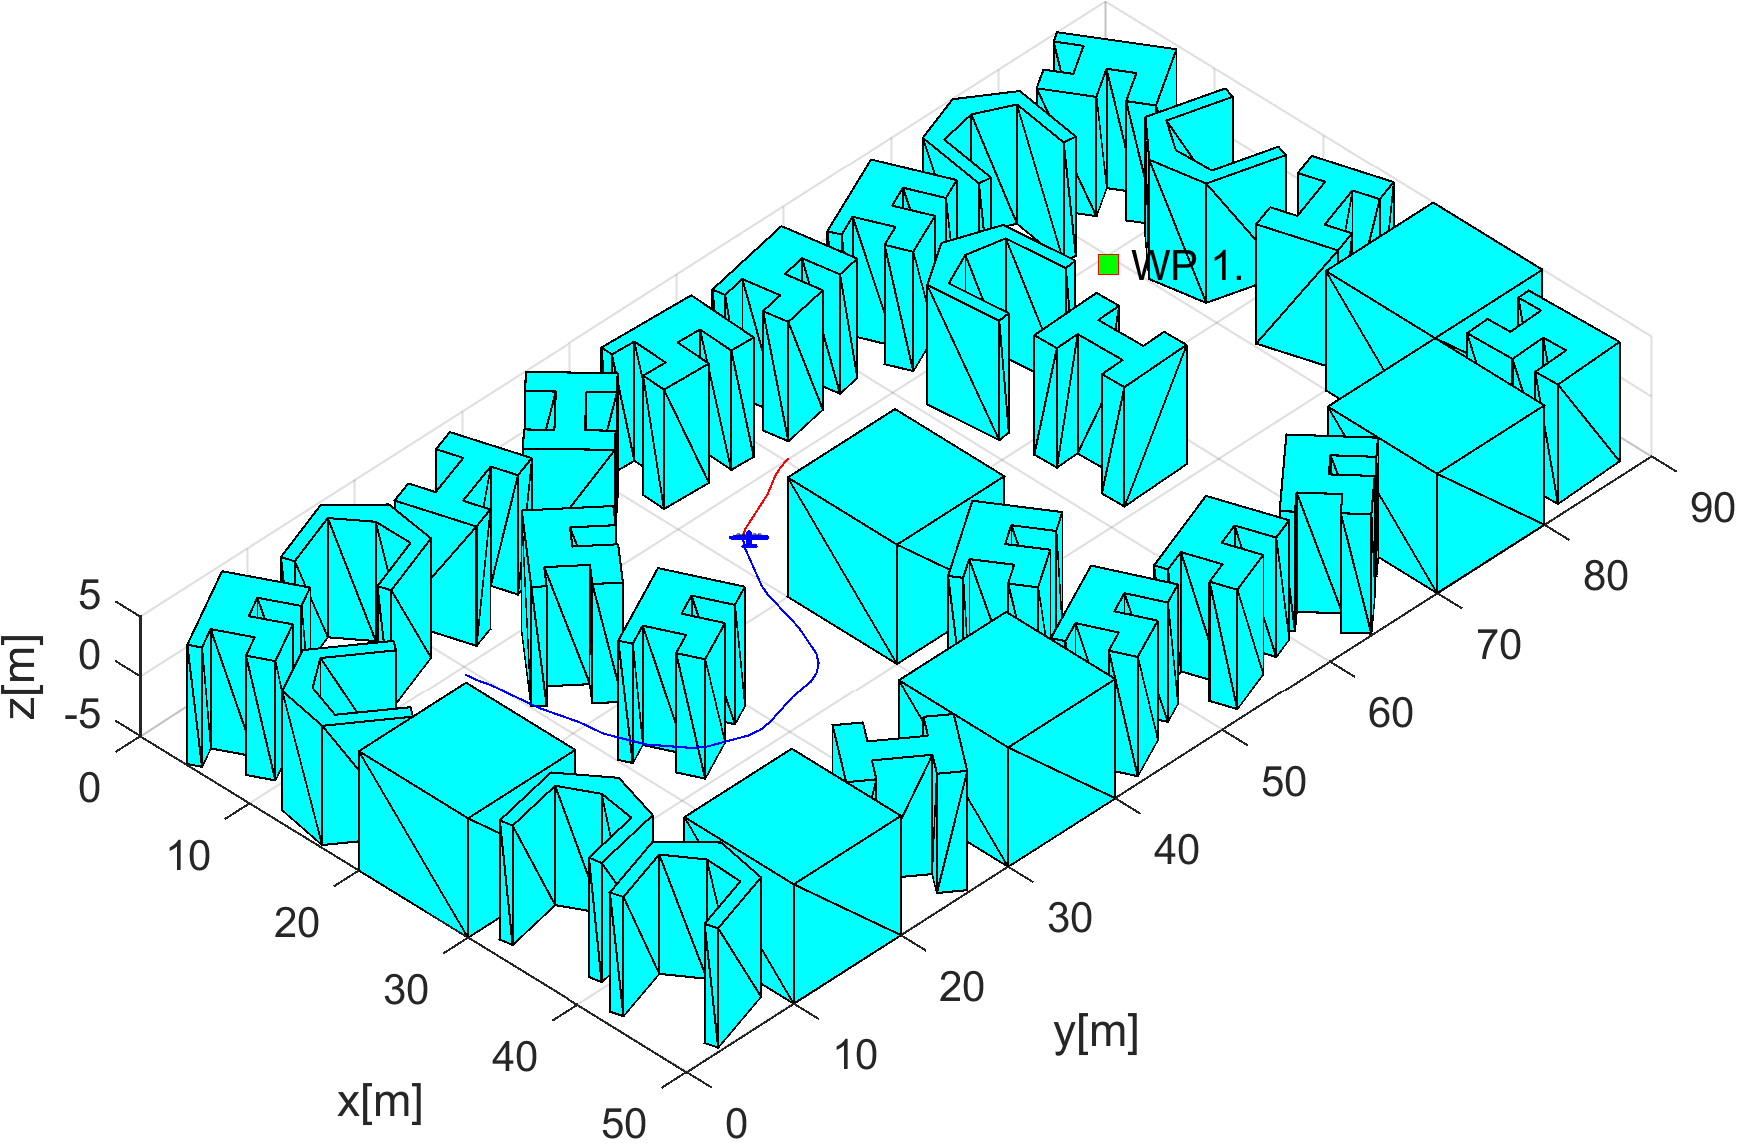
\includegraphics[width=0.9\linewidth]{\FIGDIR/NS014ConstraintsPolynomialMaze00044} 
        \caption{$2^{nd}$ turn.}
        \label{fig:mazeSecondTurn}
    \end{subfigure}
    \\
    \begin{subfigure}{0.48\textwidth}
    	\centering
        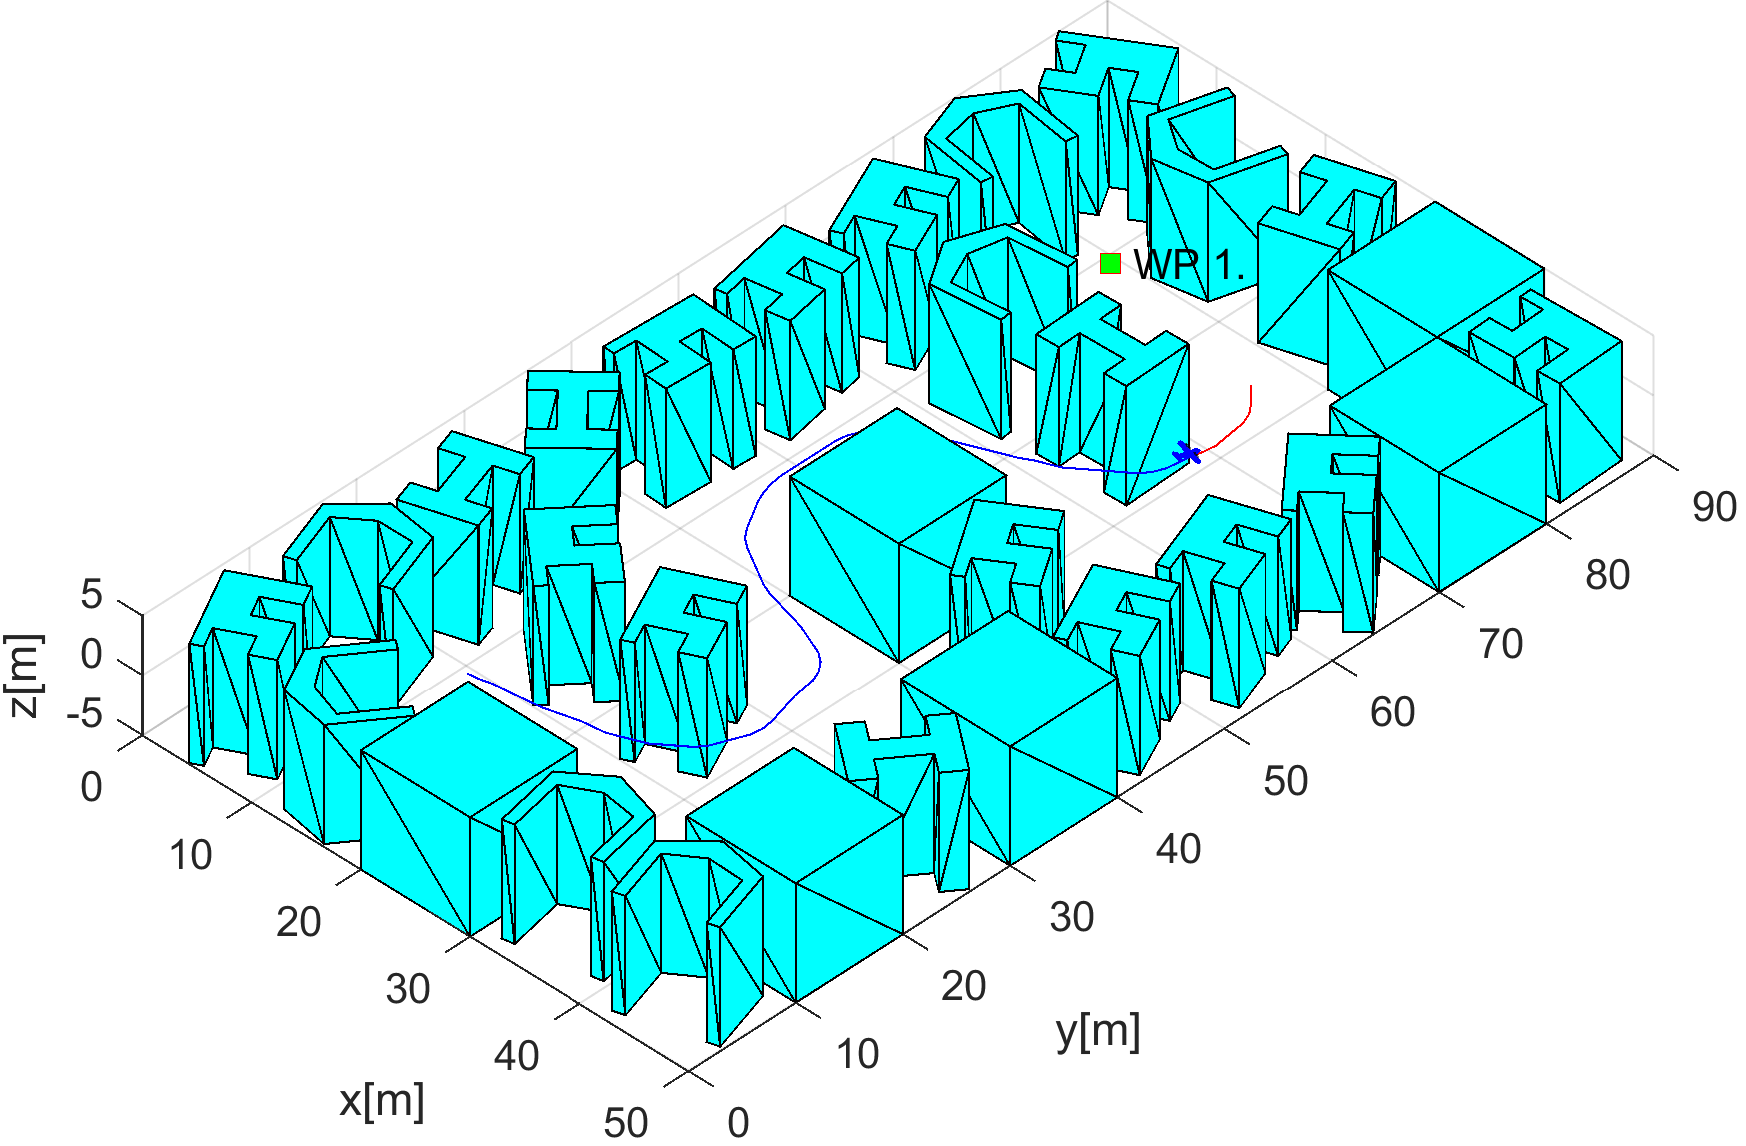
\includegraphics[width=0.9\linewidth]{\FIGDIR/NS015ConstraintsPolynomialMaze00081} 
        \caption{$3^{rd}$ turn.}
        \label{fig:mazeThirdTurn}
    \end{subfigure}
    \begin{subfigure}{0.48\textwidth}
    	\centering
        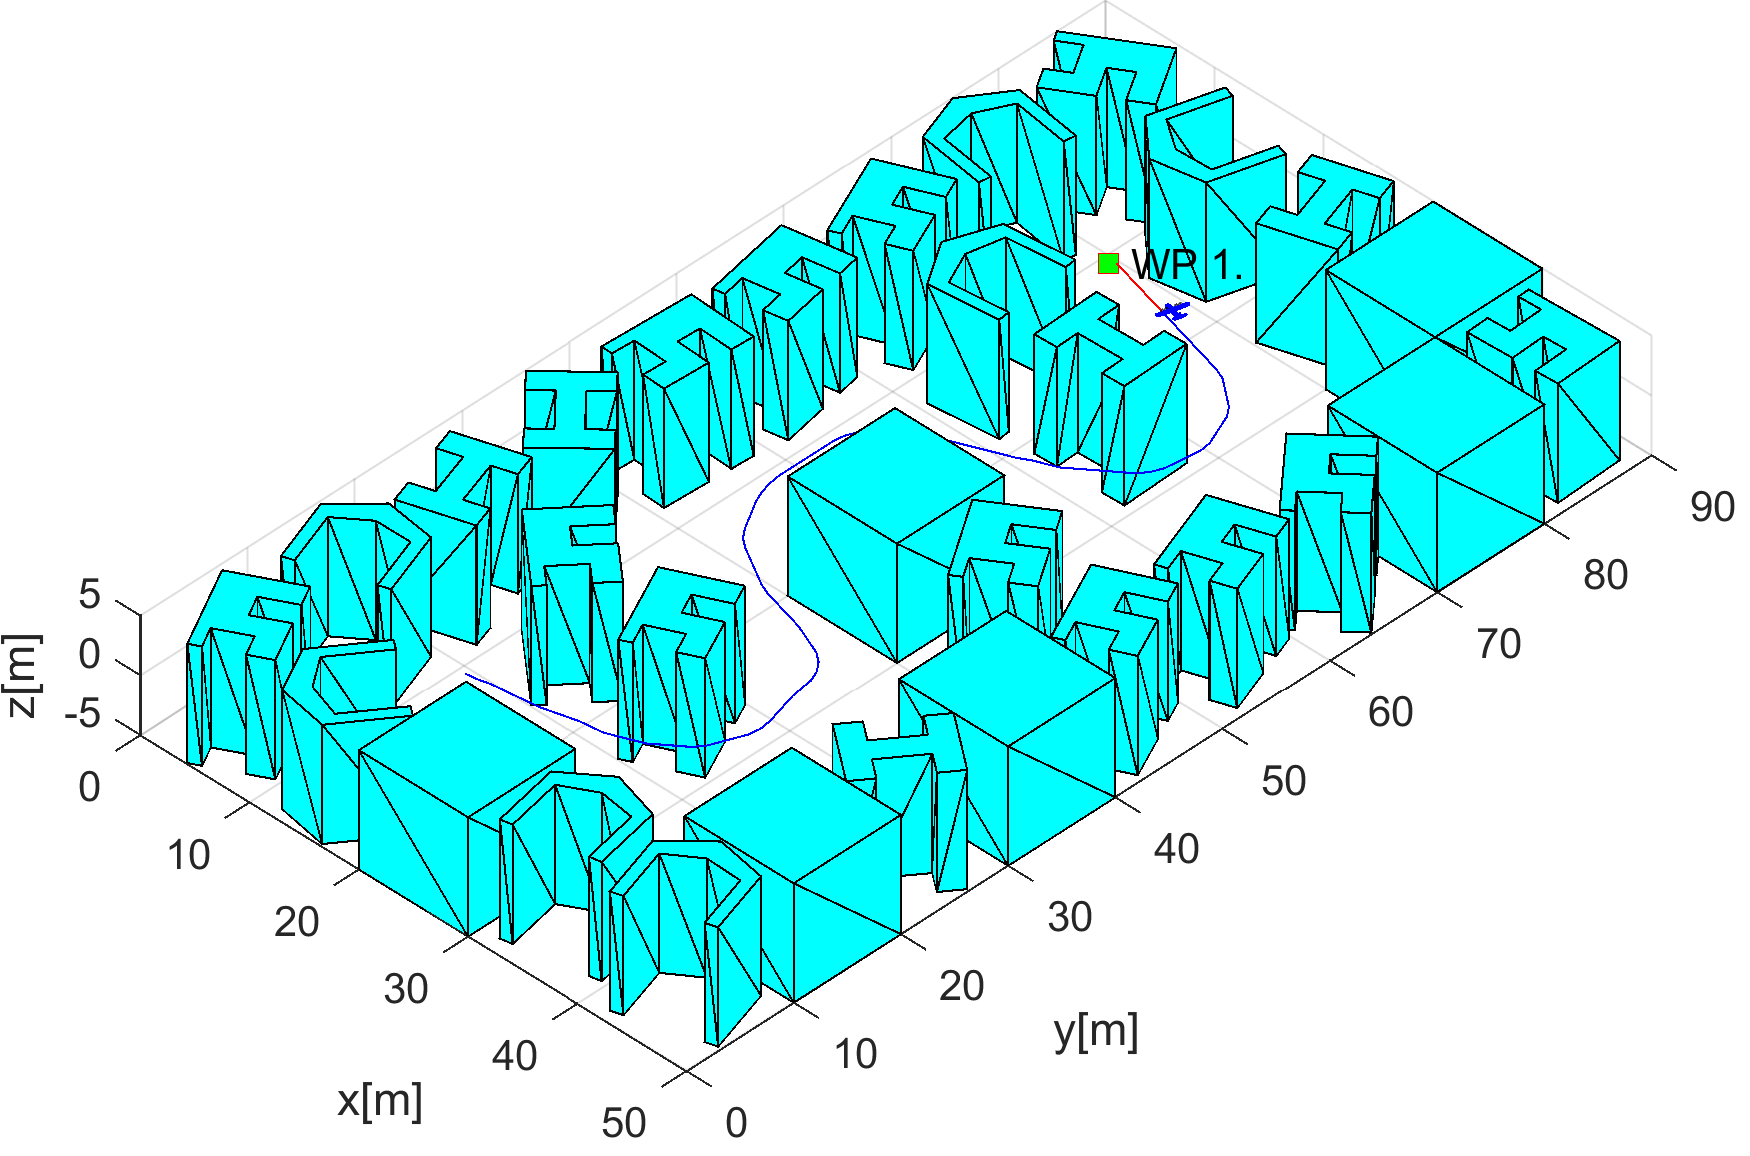
\includegraphics[width=0.9\linewidth]{\FIGDIR/NS016ConstraintsPolynomialMaze00098} 
        \caption{Waypoint reach.}
        \label{fig:mazeWaypointReach}
    \end{subfigure}
    \caption{Test scenario for \emph{Maze}. }
    \label{fig:testCaseMazeSolver}
\end{figure}

\paragraph{Distance to Body/Safety Margin Evolution:}  The evolution of \emph{body and safety margin} over time (x-axis, sec) given in  meters distance (y-axis, m) is given in (fig. \ref{fig:testCaseMazeAvoidancePerformance}).

The \emph{UAS} center distance to nearest obstacle (blue line) does not break any \emph{Safety Margin} (yellow line) of closest obstacle. \emph{Body Margin} of closest obstacle (red line) has not been break, because it always lies below of \emph{Safety Margin} (yellow).

For \emph{UTM time period} $37$ to $68$ sec there is a \emph{margin spike}  due avoidance of bloated \emph{Rectangle buildings} (fig. \ref{fig:mazeSecondTurn}) during $2^{nd}$ turn. The \emph{acceptance criterion} for \emph{Safety Margin} is satisfied.

\begin{note}
The \emph{body} and \emph{safety margin} are changing  depending on \emph{UAS position} and \emph{orientation}. The changes are reflected in (tab. \ref{tab:testCaseMazeSafetyAndBodyMarginDistances}).
\end{note}


\begin{figure}[H]
    \centering
    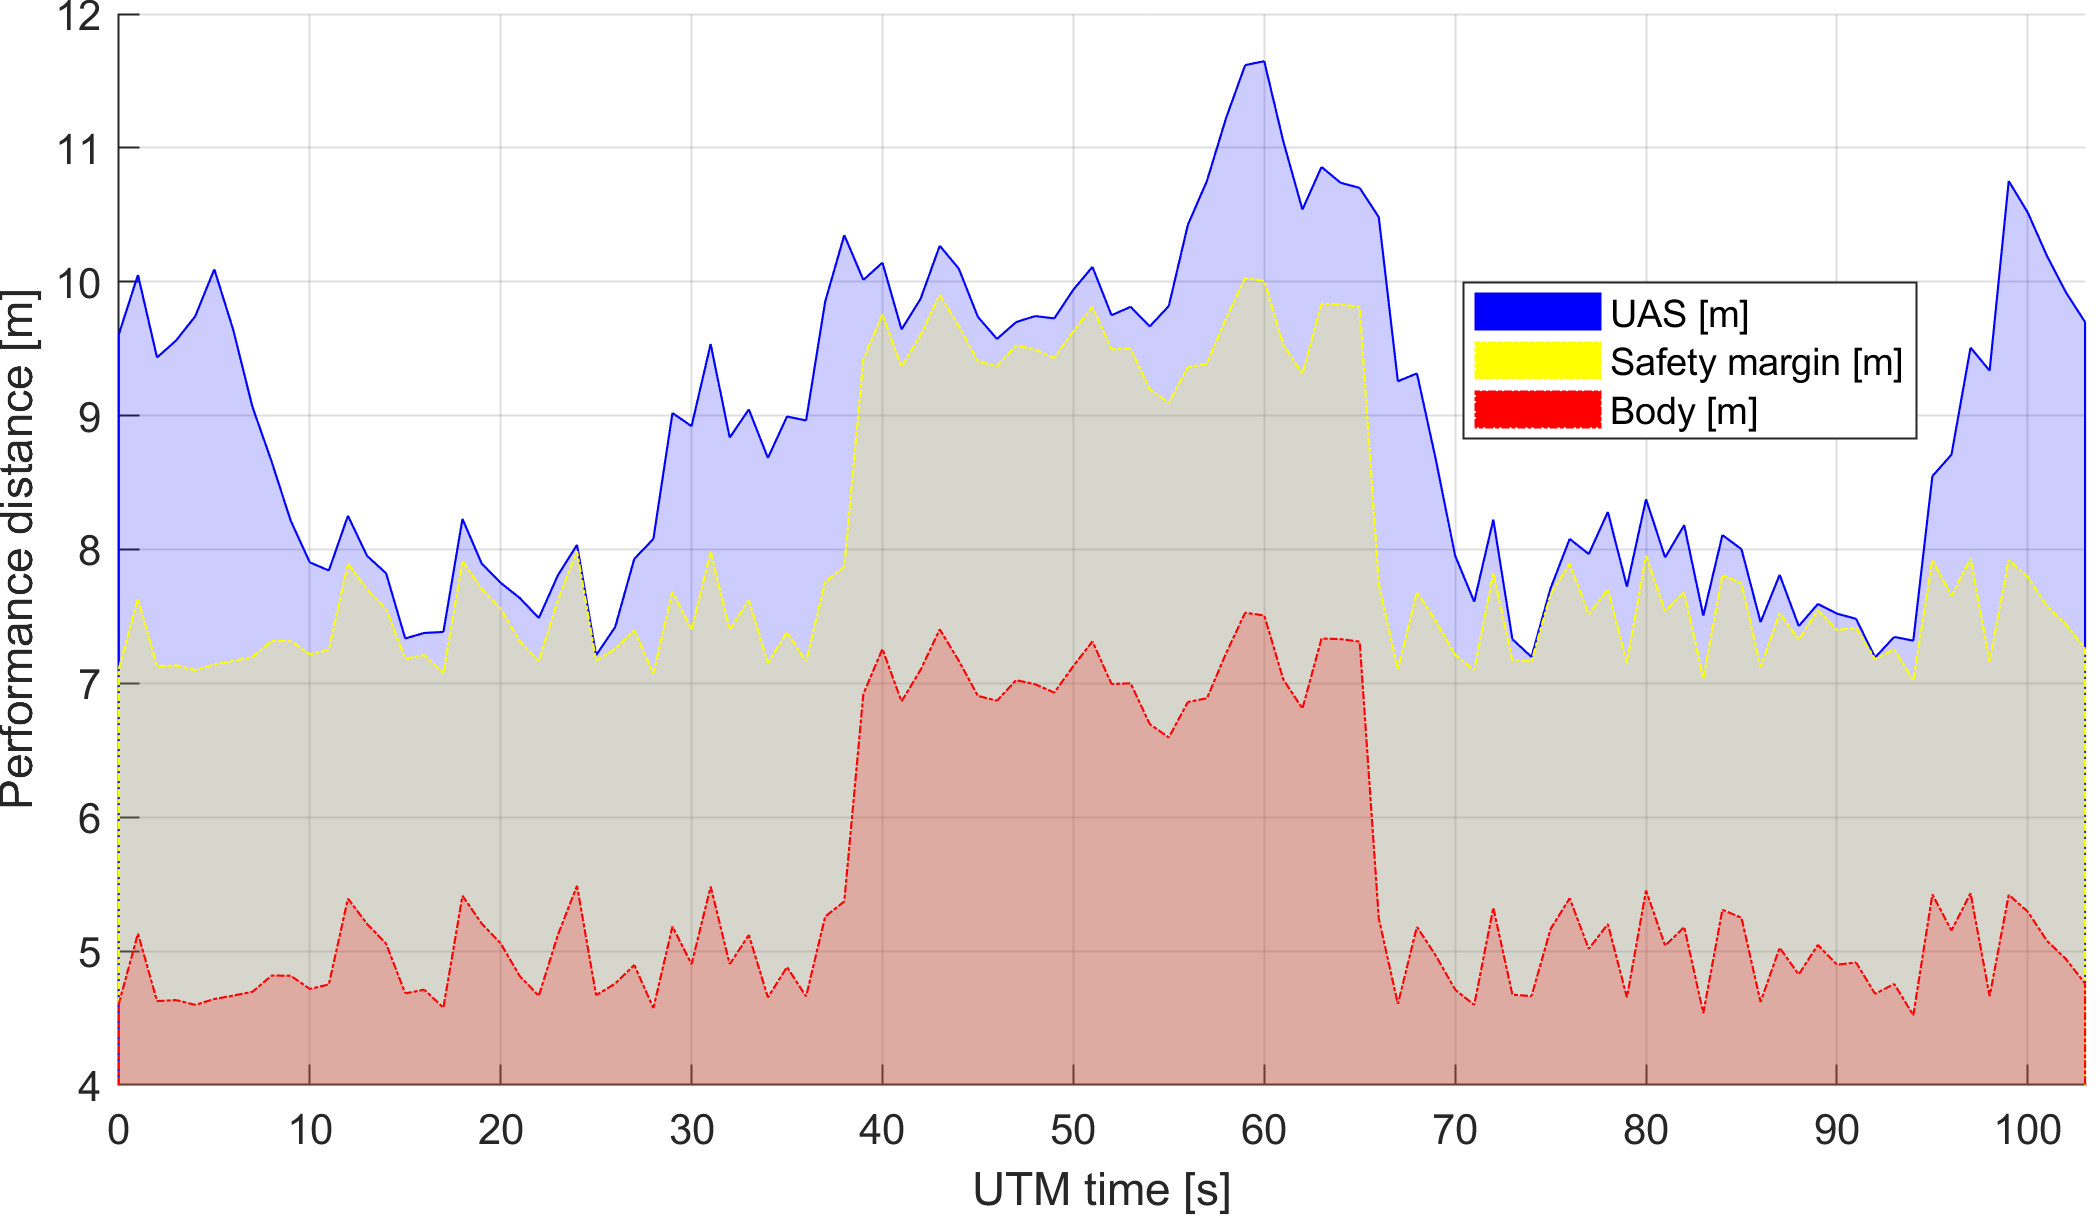
\includegraphics[width=0.8\linewidth]{\FIGDIR/NS017ConstraintsPolynomialMazePerformance} 
    \caption{Distance to body/safety margin evolution for \emph{Maze scenario}.}
    \label{fig:testCaseMazeAvoidancePerformance}
\end{figure}

\paragraph{Distance to Body/Safety Margin Peaks:} The minimal and maximal values for \emph{UAS distance} to \emph{safety margin} based on performance (fig. \ref{fig:testCaseMazeAvoidancePerformance}) is summarized in (tab. \ref{tab:testCaseMazeSafetyAndBodyMarginDistances}).

The \emph{minimal distance to safety margin} is $0.0131 m$ which can be taken as $\sim 0m$ due the numerical error. The \emph{maximal distance to safety margin} is $2.9513 m$ which is $5 \times$ \emph{UAS radius}. The safety margin distance is $\le 3 m$ which means the scenario is tightly packed with obstacles. The \emph{UAS} never left \emph{Emergency Avoidance Mode} because condition: $safety Margin Distance \ge avoidance Grid Length$ was never satisfied. 

The \emph{minimal body} distance is $5.0131 m$, while the \emph{maximal body} distance is $8.7117 m$. The difference between minimal and maximal body distance is $\sim 4 m$ which also indicates scenario packed with obstacles. 

\begin{table}[H]
    \centering
    \begin{tabular}{c|c||c}
    \multicolumn{2}{c||}{Parameter} & UAS 1 \\\hline\hline
    \multirow{2}{*}{Distance to Safety Margin} & min & 0.0131 \\\cline{2-3}
                                            & max & 2.9513 \\\hline
    \multirow{2}{*}{Distance to Body Margin}   & min & 5.0131 \\\cline{2-3}
                                            & max & 8.7117 
    \end{tabular}
    \caption{Distance to body/safety margin peaks for \emph{Maze scenario}.}
    \label{tab:testCaseMazeSafetyAndBodyMarginDistances}
\end{table}

\paragraph{Path Tracking Performance:} Reference path (green dashed) line is given as direct interconnection of \emph{initial position} (green square with S marker) and \emph{hidden waypoint} (green square with 1 marker). The \emph{UTM Reference Time} is given on x-axis. The evolution of real trajectory (blue solid line) for each axis is given as follow:

\begin{enumerate}
    \item \emph{X-axis path tracking} - reflects the maneuvering in the curves of the maze.
    
    \item \emph{Y-axis path tracking} - shows horizontal progress to the \emph{hidden goal waypoint}. The expected linear tracking is not achievement due the manuevering delays on X-axis.
    
    \item \emph{Z-axis path tracking} - shows perfect linear tracking of reference trajectory. The \emph{altitude acceptance criterion}: $-5m \le altitude \le 5m$ have been fulfilled.
\end{enumerate}

\begin{figure}[H]
    \centering
    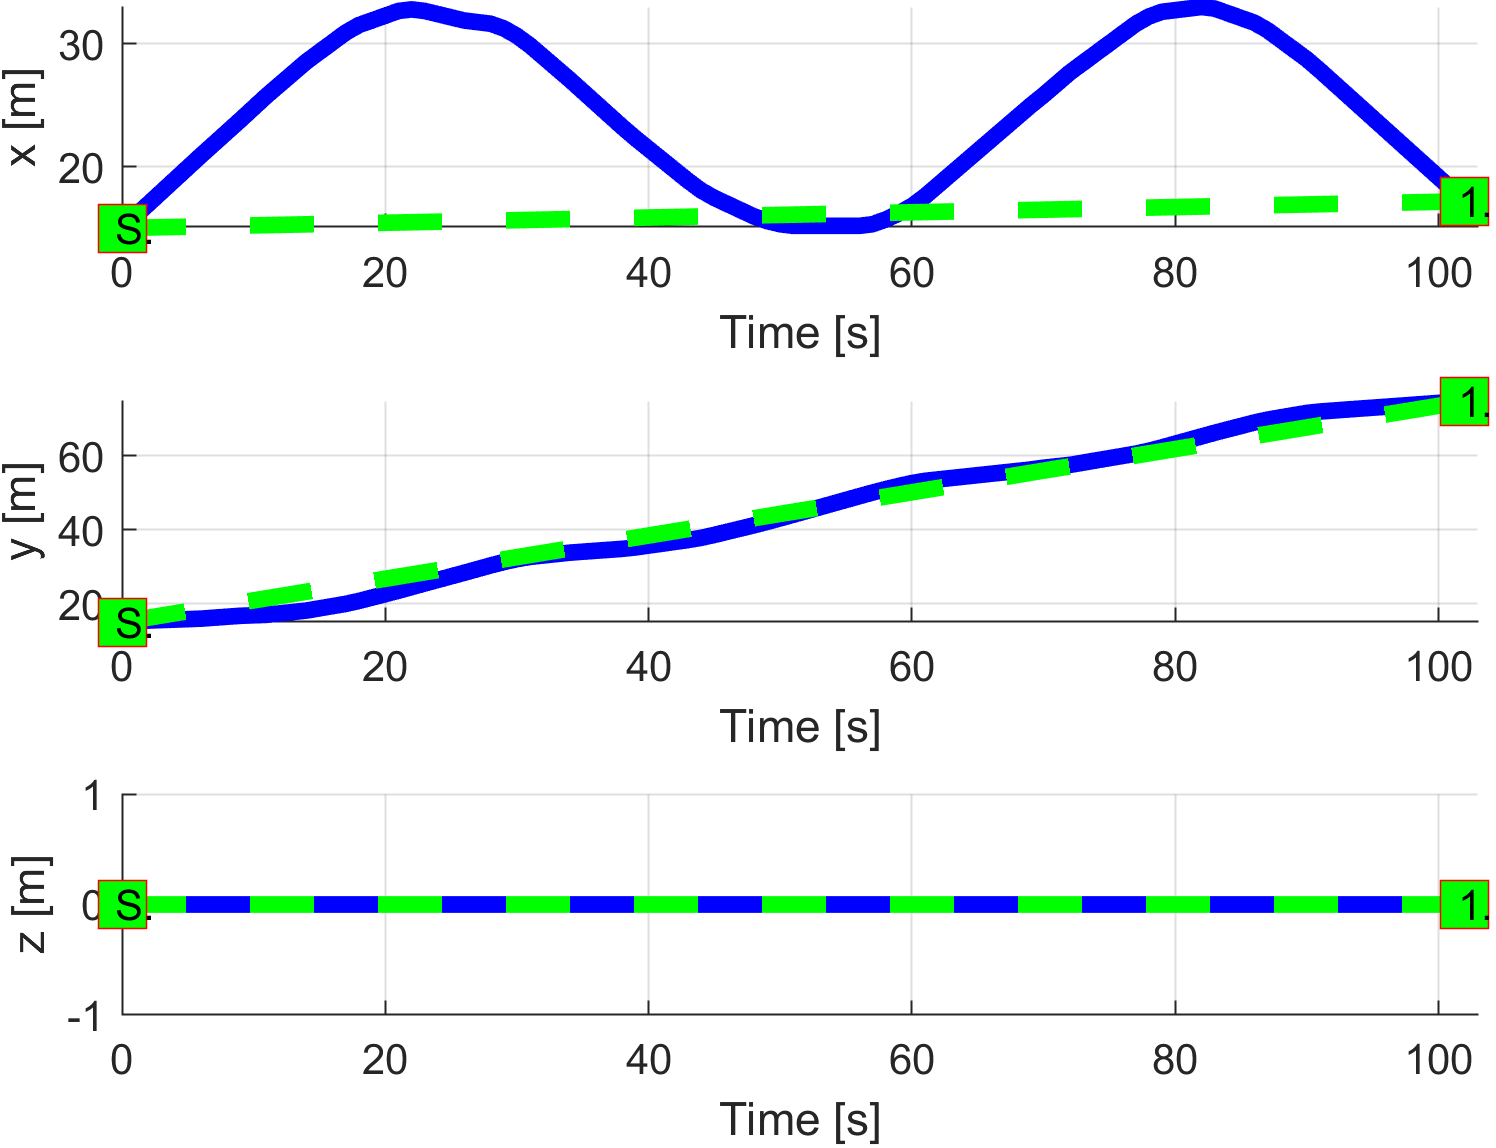
\includegraphics[width=0.55\linewidth]{\FIGDIR/NS018ConstraintsPolynomialMazePathFollowing} 
    \caption{\emph{Maze} path tracking.}
    \label{fig:testCaseMazePathTracking}
\end{figure}


\paragraph{Path Tracking Deviations:} Deviations (tab. \ref{tab:pathTrackingParametersForMazeAvoidance}) from \emph{reference trajectory} are in expected ranges considering \emph{mission plan} (tab. \ref{tab:missionSetupMazeScenario}) and \emph{obstacle properties} (tab. \ref{tab:obstacleSetMaze}).

\begin{table}[H]
    \centering
    \begin{tabular}{c||c}
        \multirow{2}{*}{Param.} & UAS 1\\\cline{2-2}
                        & $\mathscr{WP}_1$  \\\hline\hline
          $\max |x|$    & 27.32             \\\hline
          $\max |y|$    & 2.41             \\\hline
          $\max |z|$    & 0                 \\\hline
          $\max dist.$  & 28.06             \\
    \end{tabular}
    \caption{Path tracking properties for \emph{Maze} scenario.}
    \label{tab:pathTrackingParametersForMazeAvoidance}
\end{table}



    	\subsection{Storm}\label{s:testStorm}
    \paragraph{Scenario:} Small UAS is flying in open space in uncontrolled airspace ($\le$ 500 feet AGL (Above Ground Level)). A \emph{Weather Service} notices UAS about \emph{Dangerous Weather zone} (virtual constraint s. \ref{s:virtualConstraints}) which is moving in UAS direction. The \emph{UAS} is  executing mission given by (tab. \ref{tab:missionSetupStormScenario}).
    
    \begin{table}[H]
        \centering
        \begin{tabular}{c|c||c}
            \multicolumn{2}{c||}{Position} & \multirow{2}{*}{$\mathscr{WP}_1$} \\\cline{1-2}
            $[x,y,z]$           & $[\theta,\varpi,\psi]$           & \\\hline\hline
            $[0,0,0]^T $        & $[0^\circ,0^\circ,90^\circ]^T$    & $[0,60,0]^T$        \\ 
        \end{tabular}
        \caption{Mission setup for \emph{Storm} scenario.}
        \label{tab:missionSetupStormScenario}
    \end{table}
    
    \paragraph{Constraints:} The \emph{storm} is modeled as a \emph{virtual constraint} with parameters given in (tab. \ref{tab:obstacleSetStorm}). A constraint is modeled as a \emph{convex polygon} for \emph{horizontal boundary} and altitude for the \emph{vertical boundary}.
    
    The \emph{Storm} is moving through an \emph{operational region} with linear velocity $0.5 ms^{-1}$. The \emph{storm`s center} was first detected at \emph{decision frame} $0$ at position $[0,50,0]^T$.
    
    \begin{table}[H]
        \centering
        \begin{tabular}{c|c|c|c|c|c|c}
            \multicolumn{3}{c|}{Constraint} & \multicolumn{3}{c|}{Body Margin} & \multirow{2}{*}{Safety Margin}\\\cline{1-6}
            i. position & velocity & type & min. & max. & avg. &   \\\hline\hline
            $[0,50,0]^T$ & $[0,-0.5,0]$ & polygon & $9$ & $10$ & $9.5$  & $5$ \\
         \end{tabular}
        \caption{\emph{Constraint set} for \emph{Storm} scenario.}
        \label{tab:obstacleSetStorm}
    \end{table}
    
    \paragraph{Assumption:} Every \emph{avoidable moving constraint} is usually slower than an \emph{Approaching UAS}, or its radius is smaller than the turning radius of an \emph{Approaching UAS}.
    
    \begin{note}
    \emph{Manned aviation} receives a permit to operate in  \emph{controlled airspace} only if it has capability outmaneuver every known threat in requested airspace. 
    
    The \emph{Constrained space portion} is usually very large, therefore in the majority of cases the assumption $uasSpeed >> constraintSpeed$  holds.
    \end{note}
 
    \paragraph{Main Goal:} Show dynamic moving constraint avoidance capability in \emph{uncontrolled airspace}.
    
    \paragraph{Acceptance criteria:}
    \begin{enumerate}
        \item \emph{Hard constraint avoidance} - the \emph{UAS} must not cross the body margin:  $distance($ $stormCenter,$ $UAS)$ $\ge$  $bodyMargin$.
        
        \item \emph{Soft constraint avoidance} - the \emph{UAS} cannot cross the safety margin to get into proximity of \emph{Storms surrounding area}: \emph{distance(stormCenter, UAS)} $\ge$ \emph{safetyMargin}. 
    \end{enumerate}
    
    \paragraph{Testing setup:} The \emph{standard test setup} defined in (tab. \ref{tab:testMovementOrientations}, \ref{tab:testUASBasicParameters}, \ref{tab:testNavigationGridBasic}, \ref{tab:testAvoidanceGridBasic}, \ref{tab:testUASColoring}) is used with following parameter override:
    \begin{enumerate}
        \item \emph{Avoidance grid - type} - \emph{ACAS-like} with \emph{horizontal enabled maneuvers}.
    \end{enumerate}
    
    \paragraph{Simulation run:} \emph{Notable moments} from a \emph{simulation run} (fig. \ref{fig:testCaseStormAvoidance}) are the following:
    \begin{enumerate}
    
        \item \emph{Detection} (fig. \ref{fig:stromSituationDetection}) - the \emph{Storm} (magenta polygon) is detected prior to the engagement (retrieved from associated weather service). The \emph{UAS} (blue) stays in \emph{Navigation mode}. \emph{Trajectories} in \emph{Navigation grid} are constrained by rule \emph{Enforce safety margin} (tab. \ref{tab:ruleEnforceSafetyMargin}). The \emph{Planned trajectory} (red) changes to avoid \emph{Storm}.
        
        \item \emph{Avoidance start} (fig. \ref{fig:stormAvoidanceStart}) - when UAS reaches optimal avoidance distance, the \emph{navigation reach set} is constrained, forcing UAS to perform an evasive maneuver.
        
        \item \emph{Avoidance end} (fig. \ref{fig:stormAvoidanceEnd}) - navigation space is no longer constrained when the \emph{minimal safe distance/heading} is achieved.
        
        \item \emph{Waypoint reached} (fig. \ref{fig:stormWaypointReach}) - standard waypoint navigation procedure was used in this case.
        
    \end{enumerate}
        
    \begin{figure}[H]
        \centering
        \begin{subfigure}{0.48\textwidth}
        	\centering
            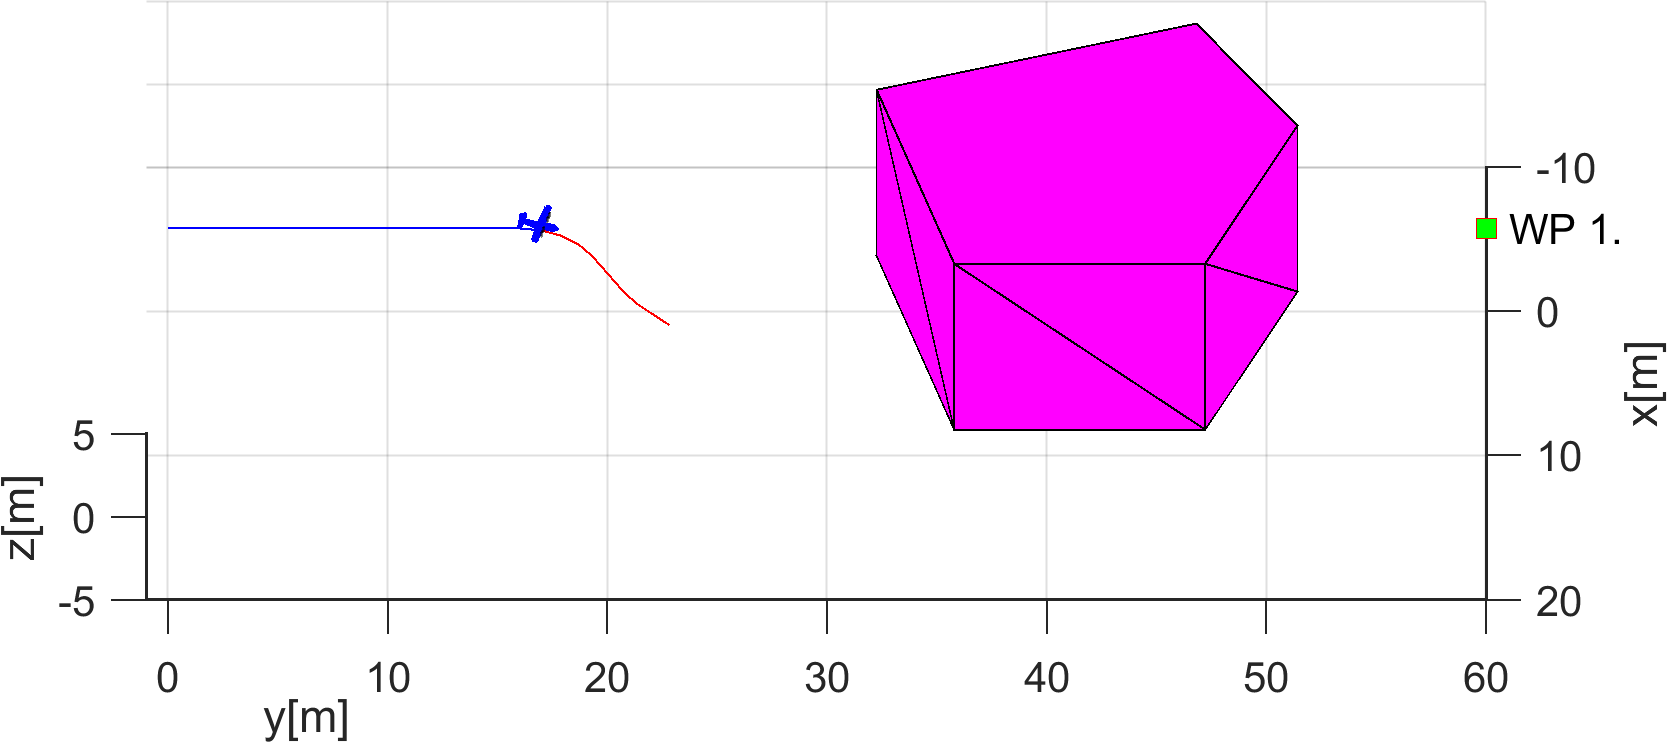
\includegraphics[width=0.9\linewidth]{\FIGDIR/NS019ConstraintsPolynomialStorm00017}
            \caption{Situation detection.}
            \label{fig:stromSituationDetection}
        \end{subfigure}
        \begin{subfigure}{0.48\textwidth}
        	\centering
            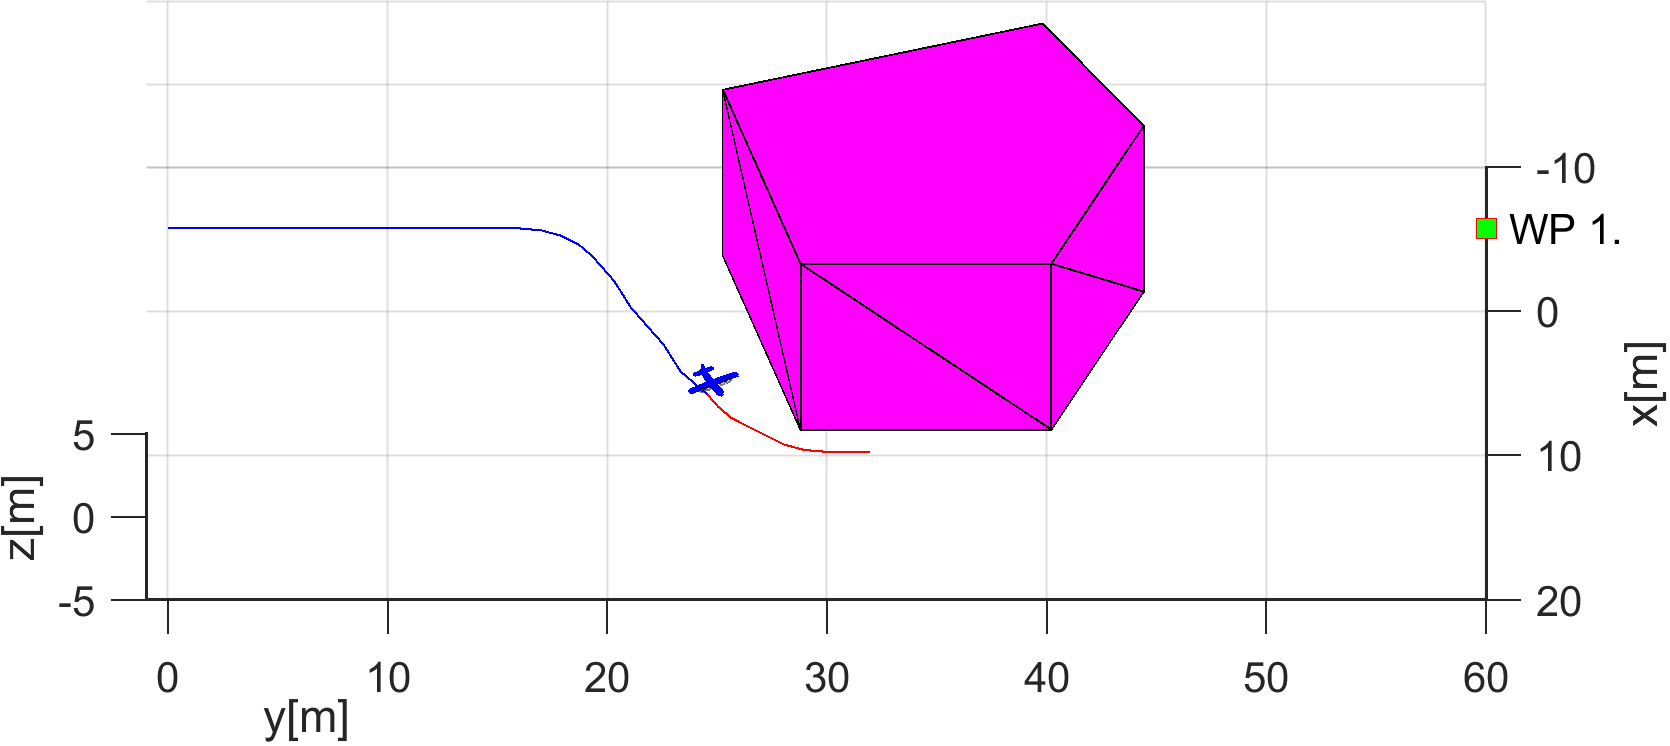
\includegraphics[width=0.9\linewidth]{\FIGDIR/NS020ConstraintsPolynomialStorm00031} 
            \caption{Storm avoidance start.}
            \label{fig:stormAvoidanceStart}
        \end{subfigure}
        \\
        \begin{subfigure}{0.48\textwidth}
        	\centering
            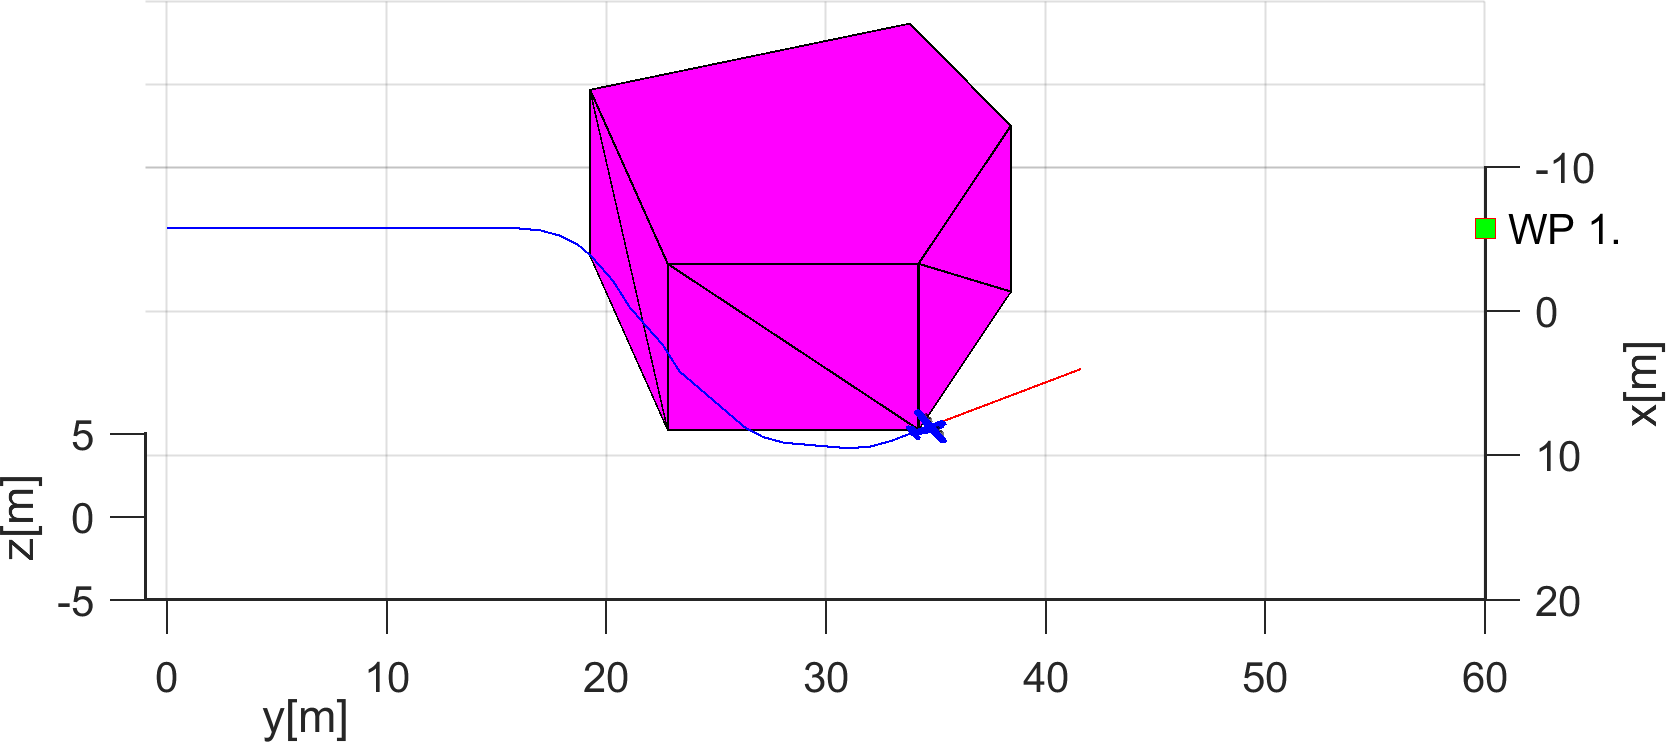
\includegraphics[width=0.9\linewidth]{\FIGDIR/NS021ConstraintsPolynomialStorm00043} 
            \caption{Storm avoidance end.}
            \label{fig:stormAvoidanceEnd}
        \end{subfigure}
        \begin{subfigure}{0.48\textwidth}
        	\centering
            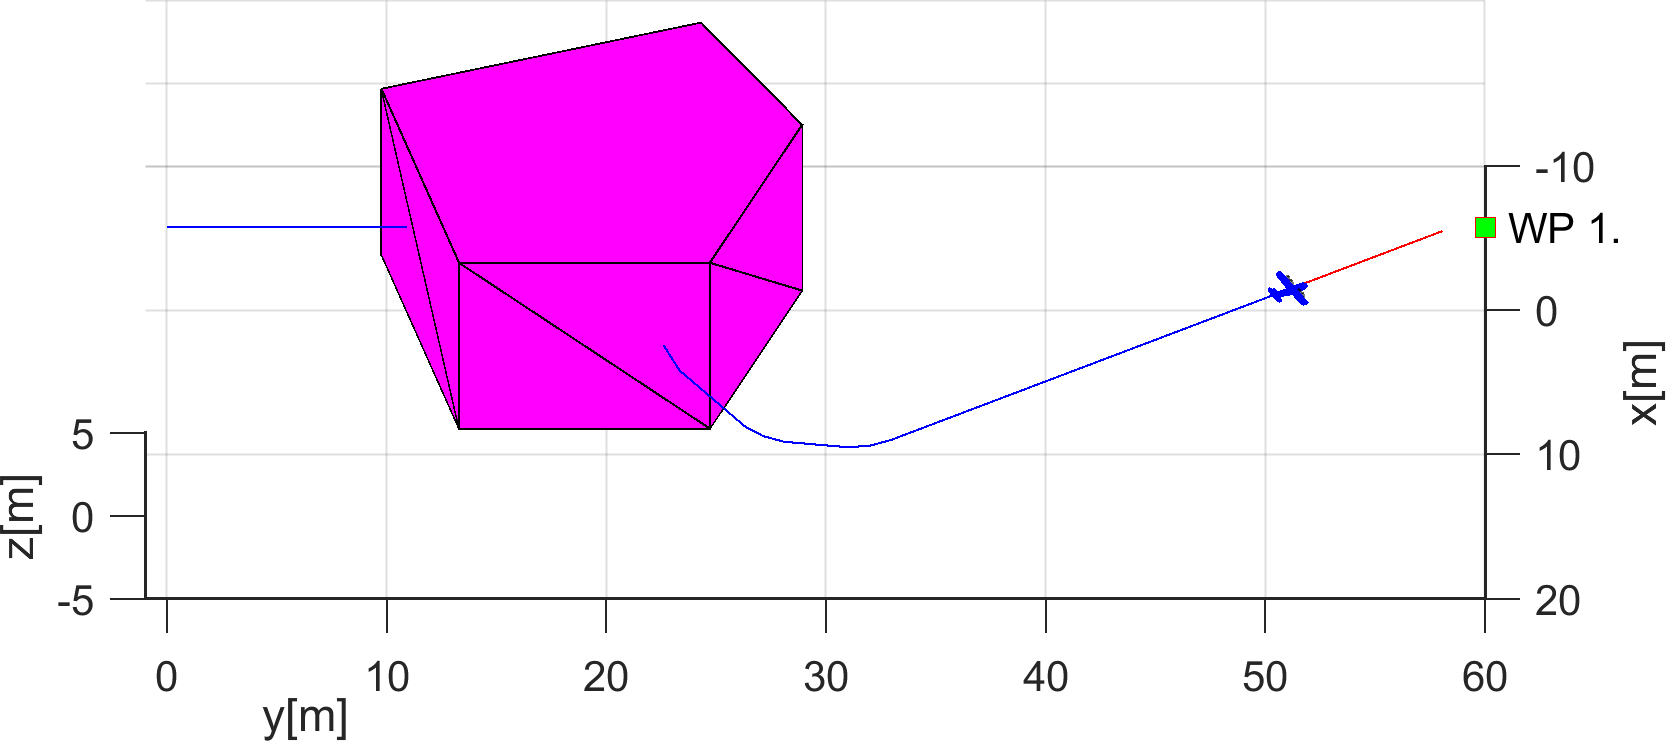
\includegraphics[width=0.9\linewidth]{\FIGDIR/NS022ConstraintsPolynomialStorm00062} 
            \caption{Waypoint reach.}
            \label{fig:stormWaypointReach}
        \end{subfigure}
        \caption{Test scenario for \emph{Storm} (Dynamic hard constraint). }
        \label{fig:testCaseStormAvoidance}
    \end{figure}
    
    \paragraph{Distance to Body/Safety Margin Evolution:} The \emph{body margin} (red line) and \emph{safety margin} (yellow line) and \emph{UAS distance to storm center} (blue line) evolution over \emph{UTM time} (x-axis) are given in (fig. \ref{fig:testCaseStormAvoidancePerformance}) The \emph{body} and \emph{safety} margin was changing according to the mutual position of the \emph{storm} and the \emph{UAS} (see tab. \ref{tab:obstacleSetStorm}). 
    
    The acceptance criteria for the \emph{hard constraint avoidance} and \emph{soft constraint avoidance} have been fulfilled. 
    
    \begin{figure}[H]
        \centering
        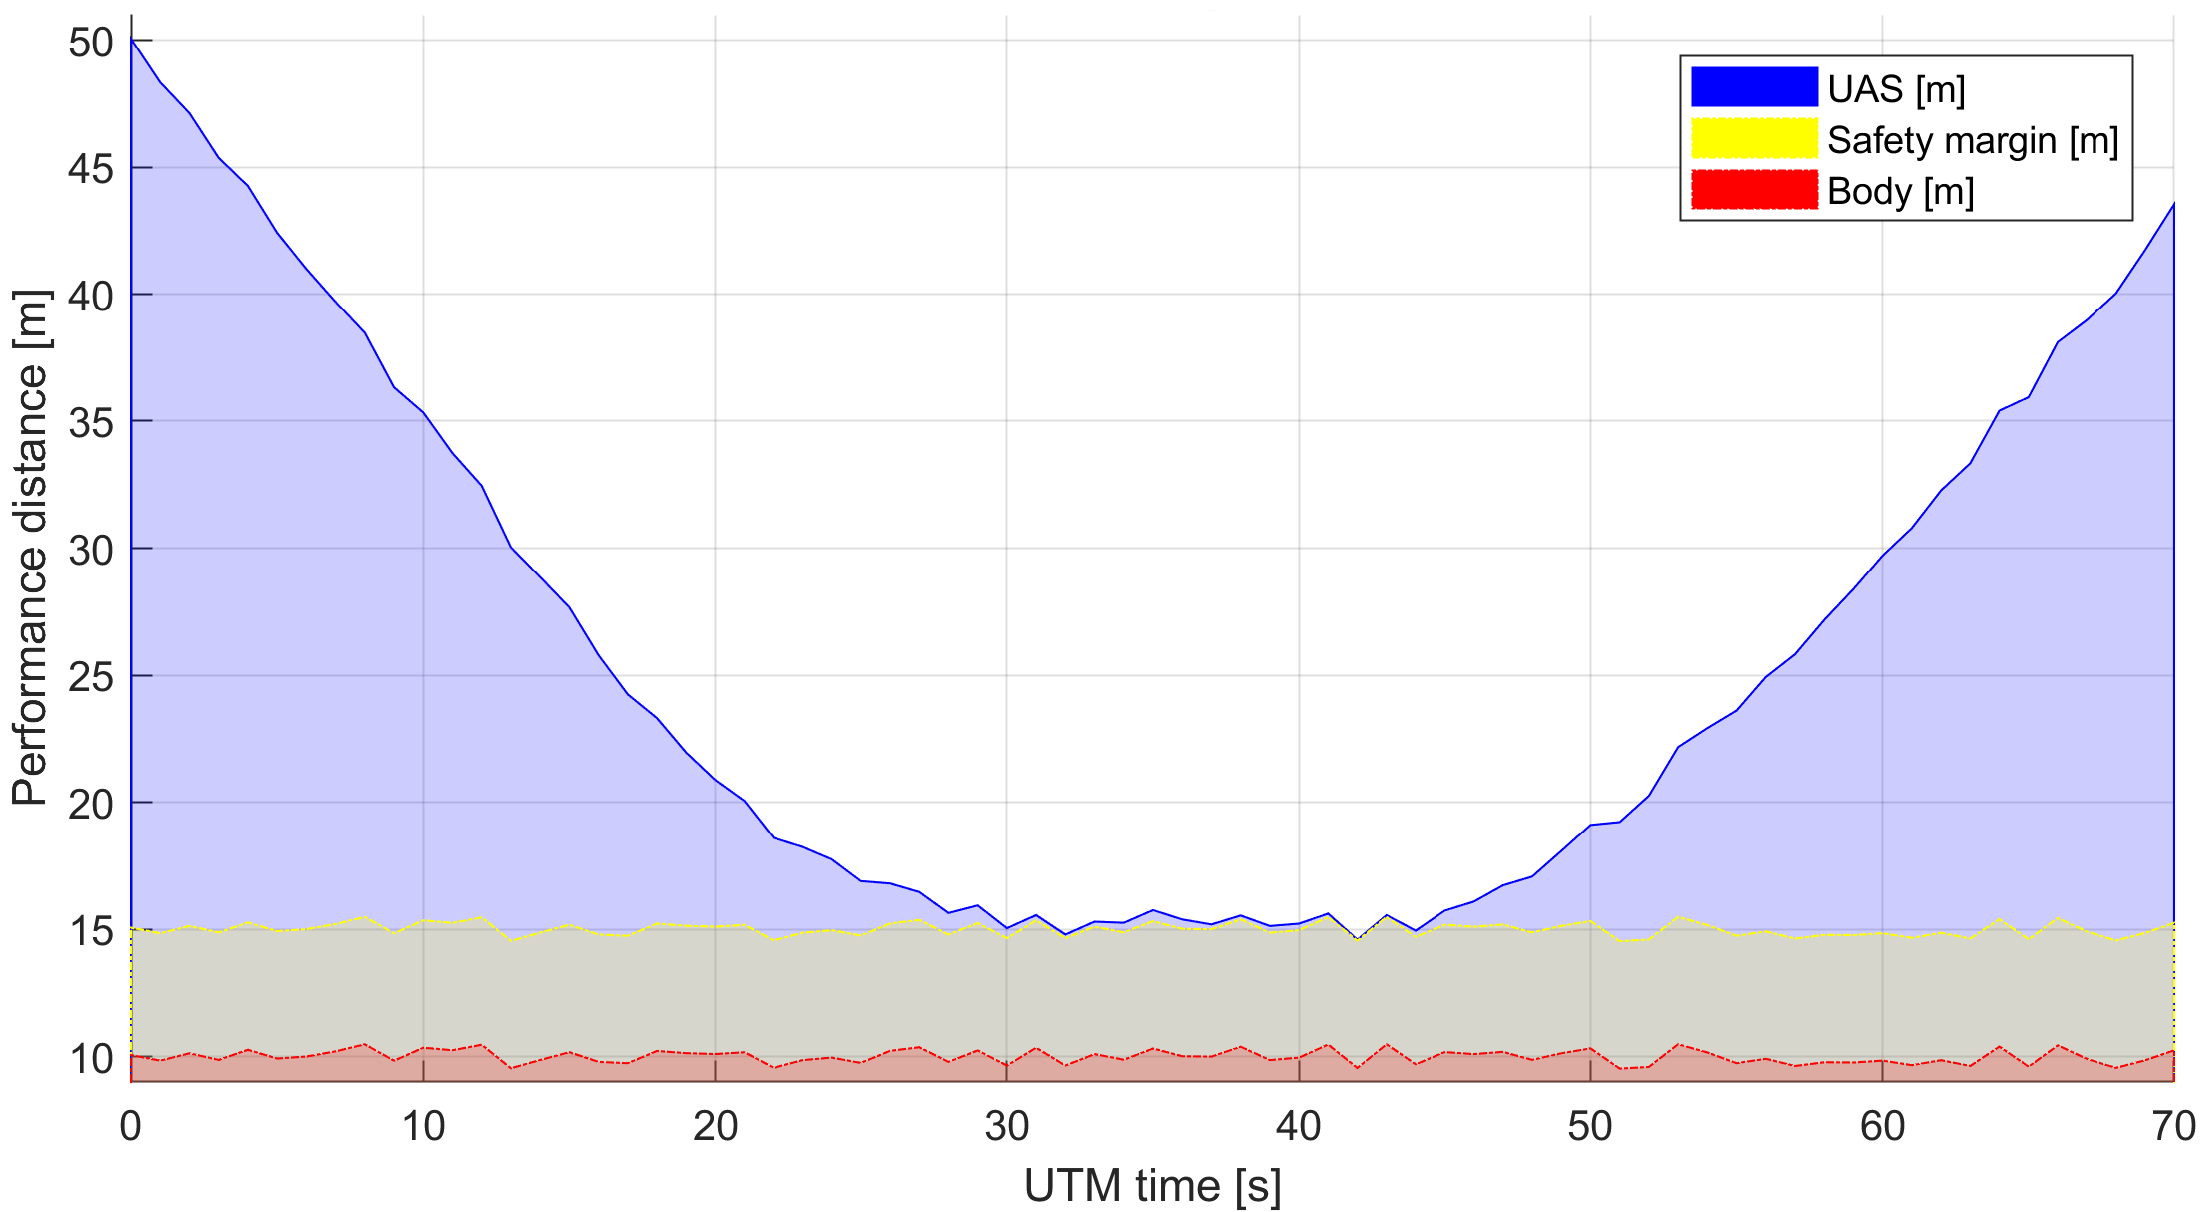
\includegraphics[width=0.8\linewidth]{\FIGDIR/NS023ConstraintsPolynomialStormPerformance} 
        \caption{Distance to body/safety margin evolution for \emph{Storm scenario}.}
        \label{fig:testCaseStormAvoidancePerformance}
    \end{figure}
    
    
    \paragraph{Distance to Body/Safety Margin Peaks:} A \emph{hard constraint} of \emph{body margin} was not breached, because the \emph{distance(UAS(t),stormBody(t))} was all time greater than \emph{0}. Thus the \emph{UAS} stayed well clear from \emph{Storm}. The summary (tab. \ref{tab:testCaseStormSafetyAndBodyMarginDistances}) shows that the \emph{minimal body margin distance} was $5.0335$ $m$, which proves \emph{avoidance of hard constraint}.
    
    A \emph{soft constraint} represented as a \emph{safety margin} (protective coating around storm body) was not breached, because the \emph{distance(UAS(t), stormBody(t)) - safetyMargin(t)} was all time greater than \emph{0}.  The summary (tab. \ref{tab:testCaseStormSafetyAndBodyMarginDistances}) show that the \emph{minimal safety margin distance} was $0.0355$ $m$, which proves \emph{avoidance of soft constraints}.
    
    \begin{table}[H]
        \centering
        \begin{tabular}{c|c||c}
        \multicolumn{2}{c||}{Parameter} & UAS 1 \\\hline\hline
        \multirow{2}{*}{Distance to Safety Margin} & min & 0.0355 \\\cline{2-3}
                                                & max & 34.9934 \\\hline
        \multirow{2}{*}{Distance to Body Margin}   & min & 5.0355 \\\cline{2-3}
                                                & max & 39.9934 
        \end{tabular}
        \caption{Distance to body/safety margin peaks for \emph{Storm scenario}.}
        \label{tab:testCaseStormSafetyAndBodyMarginDistances}
    \end{table}
    
    \paragraph{Path Tracking Performance:} The \emph{path tracking} (solid blue line) of \emph{reference trajectory} (green dashed line) between \emph{starting waypoint} (green square marked "S") and \emph{final waypoint} (green square marked "1") is portrayed in (fig. \ref{fig:testCaseStormPathTracking}). The\emph{UAS} executes \emph{horizontal right-side avoidance} of the \emph{Storm} as is preferred. 
    
    \begin{figure}[H]
        \centering
        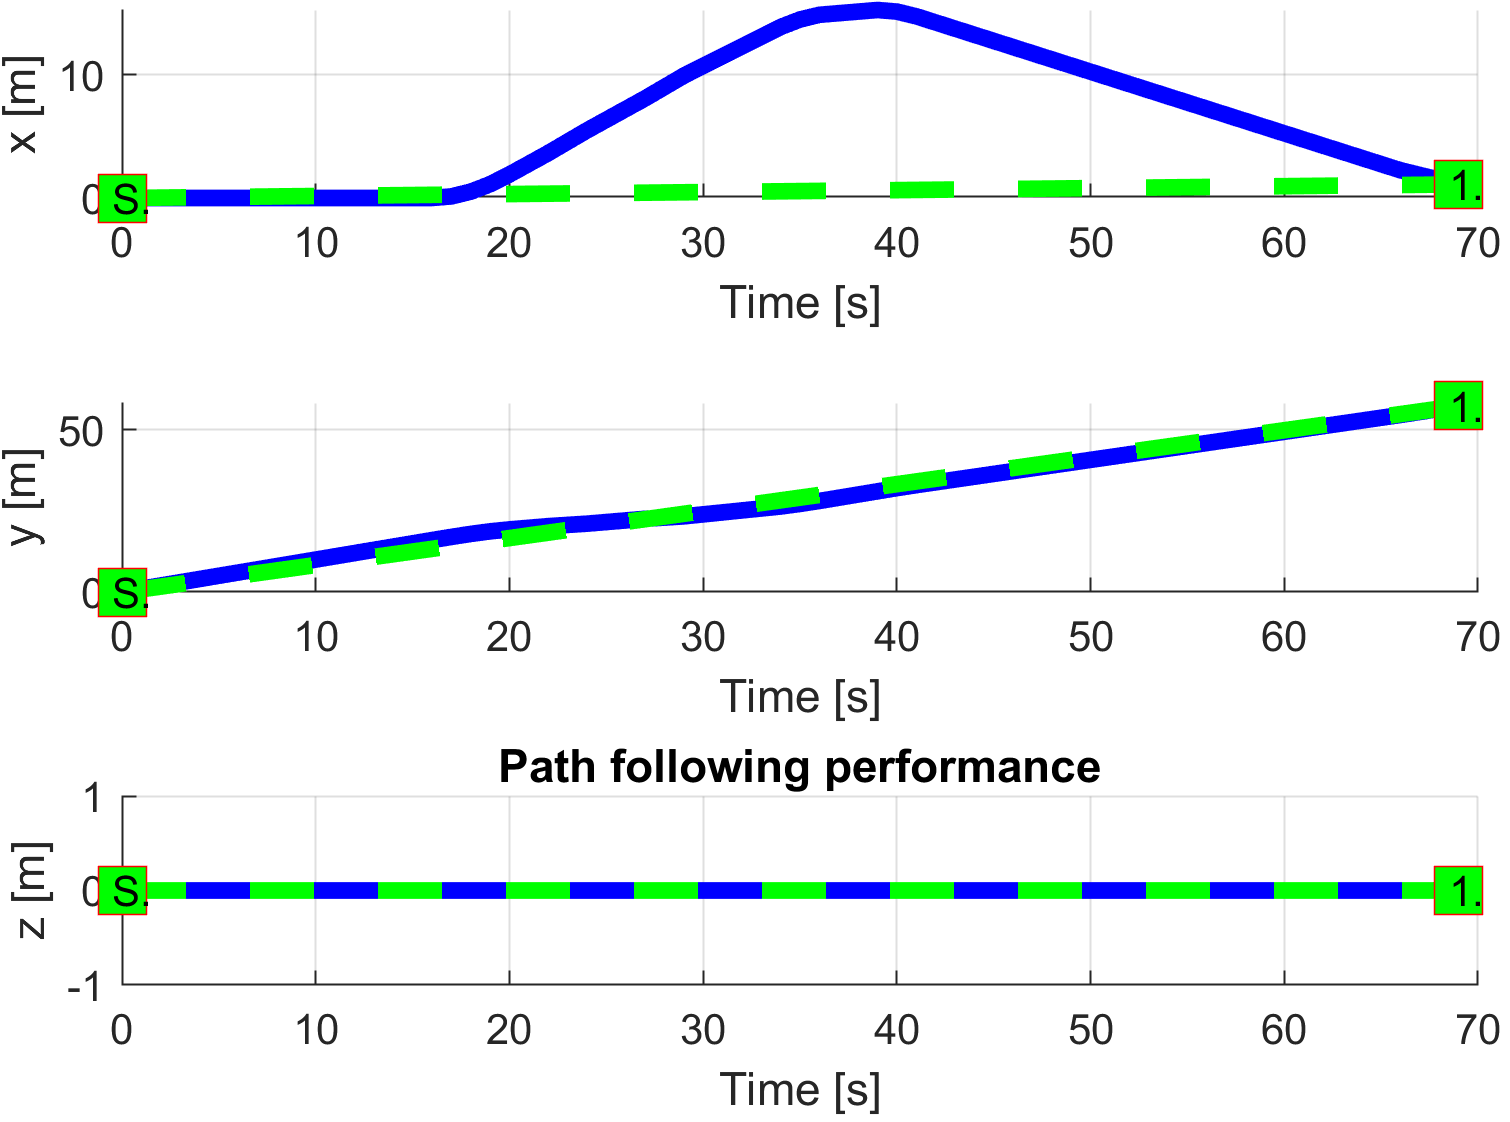
\includegraphics[width=0.55\linewidth]{\FIGDIR/NS024ConstraintsPolynomialStormPathFollowing} 
        \caption{\emph{Storm} avoidance scenario path tracking.}
        \label{fig:testCaseStormPathTracking}
    \end{figure}
    
    \paragraph{Path Tracking Deviations:} \emph{Deviations} (tab. \ref{tab:pathTrackingParametersForStormAvoidance}) are in expected ranges considering the mission plan (tab. \ref{tab:missionSetupStormScenario}) and \emph{body} and \emph{safety} margins (tab. \ref{tab:obstacleSetStorm}).
    
    \begin{table}[H]
        \centering
        \begin{tabular}{c||c}
            \multirow{2}{*}{Param.} & UAS 1\\\cline{2-2}
                            & $\mathscr{WP}_1$  \\\hline\hline
              $\max |x|$    & 15.26             \\\hline
              $\max |y|$    & 1.32             \\\hline
              $\max |z|$    & 0                 \\\hline
              $\max dist.$  & 15.76             \\
        \end{tabular}
        \caption{Path tracking properties for \emph{Storm} scenario.}
        \label{tab:pathTrackingParametersForStormAvoidance}
    \end{table}
    
    
    % 04 Storm
\paragraph{Computation Load:} The \emph{computation load} for \emph{scenario} (fig.\ref{fig:stormComputationTime}) shows used time (y-axis) over decision frame (x-axis).

The \emph{computation time} is low; it only increases slightly during  avoidance maneuver.

\begin{figure}[H]
    \centering
    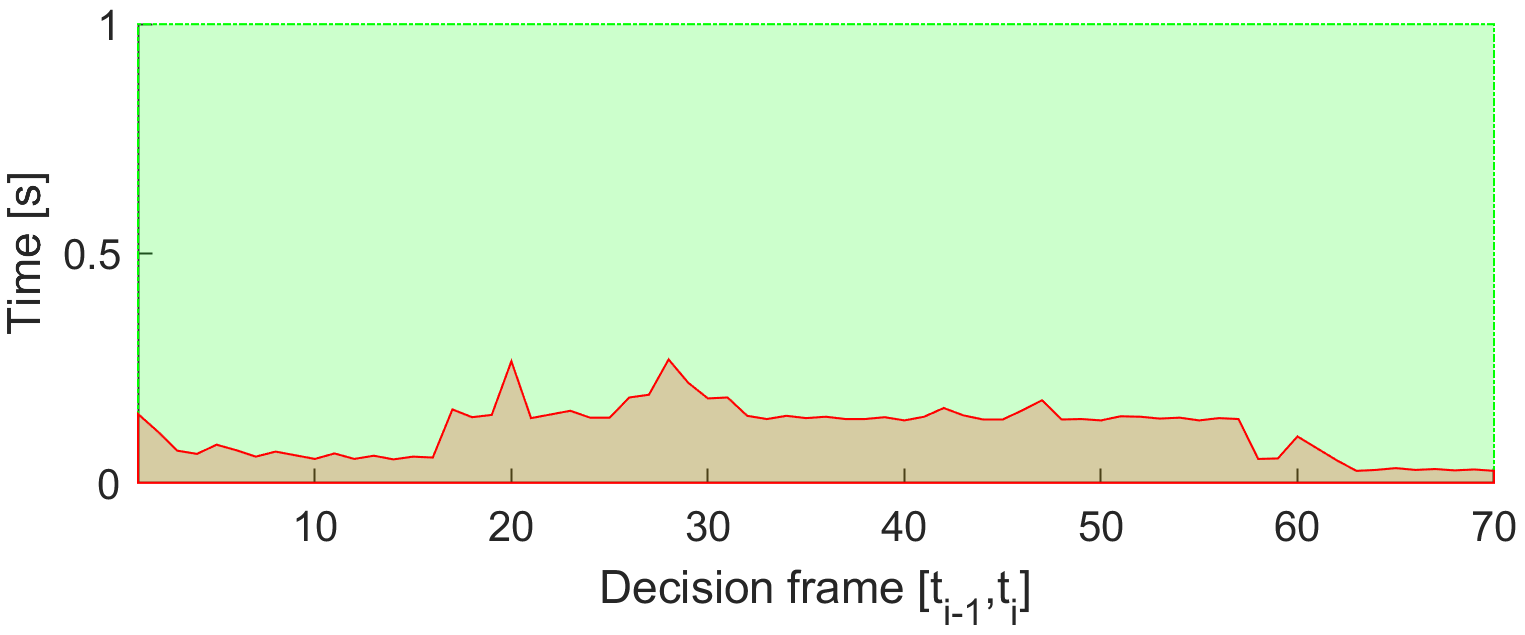
\includegraphics[width=0.65\linewidth]{\FIGDIR/NS095StormComputationTime} 
    \caption{Computation time for \emph{Maze} scenario.}
    \label{fig:stormComputationTime}
\end{figure}
    
    

    	\subsection{Emergency Converging}\label{s:testEmergencyConverging}

\paragraph{Scenario:} Two \emph{UAS} are flying in  \emph{uncontrolled airspace} (altitude $\le$ 500 ft. Above the Ground Level) with missions defined in (tab. \ref{tab:missionSetupEmergencyConvergingScenario}). Both \emph{UAS} are in the \emph{Navigation mode} with active \emph{ADSB-In/Out}, receiving position notification from each other. Cruising altitude is sufficient for horizontal separation (50-100 ft. Above the Ground Level). \emph{Horizontal separation} is the preferred separation type for both \emph{UAS}.

\begin{table}[H]
    \centering
    \begin{tabular}{c||c|c||c}
        \multirow{2}{*}{UAS} &\multicolumn{2}{c||}{Position} & \multirow{2}{*}{$\mathscr{WP}_1$} \\\cline{2-3}
          & $[x,y,z]$           & $[\theta,\varpi,\psi]$           & \\\hline\hline
        1 & $[0,20,0]^T $       & $[0^\circ,0^\circ,0^\circ]^T$    & $[40,20,0]^T$\\\hline 
        2 & $[20,0,0]^T $       & $[0^\circ,0^\circ,90^\circ]^T$  & $[20,40,0]^T$\\ 
    \end{tabular}
    \caption{Mission setup for \emph{Emergency converging} scenario.}
    \label{tab:missionSetupEmergencyConvergingScenario}
\end{table}

\begin{note}
\emph{Collision point} is expected at $\mathscr{C} = [20,20,0]^T$. The \emph{angle of approach} is $90^{\circ}$ which classifies the  situation as \emph{Converging maneuver} (fig. \ref{fig:OvertakeManeuverTheoretical}).
\end{note}

\paragraph{Main Goal:} Show two \emph{non-cooperative} UAS avoidance capability for \emph{Converging maneuver} scenario in \emph{uncontrolled airspace}.


\paragraph{Acceptance criteria:}
\begin{enumerate}
    \item \emph{Proper mode invocation} - when an intruder intersects the UAS  with \emph{Right of the Way} navigation grid, both UAS will switch into \emph{Emergency Avoidance Mode}.
    
    \item \emph{Minimal safety margin distance} $\ge$ $0 m$.
    
    \item \emph{Each UAS} will reach own goal waypoint (tab. \ref{tab:missionSetupEmergencyConvergingScenario}).
\end{enumerate}

\paragraph{Testing setup:} The \emph{standard test setup} for each UAS defined in (tab \ref{tab:testMovementOrientations}, \ref{tab:testUASBasicParameters}, \ref{tab:testNavigationGridBasic}, \ref{tab:testAvoidanceGridBasic}, \ref{tab:testUASColoring}) is used with the following without parameter override.

\emph{Intruder intersection} model has been chosen depending on UAS (tab. \ref{tab:aboidanceParametersForEmergencyConvergingScenario}). Each UAS is equipped with \emph{ADS-B In/Out} sensor obtaining/distributing the following information:

\begin{enumerate}
    \item \emph{Position} - in operational section coordinate frame.

    \item \emph{Velocity} - vector representation in the given coordinate frame.

    \item \emph{Class size} - class body radius based on UAS propulsion and size.

    \item \emph{Safety margin set} - set of safety margins for different collision cases.
\end{enumerate}

\noindent \emph{Avoidance parameters} for the \emph{Emergency converging scenario} are given in (tab. \ref{tab:aboidanceParametersForEmergencyConvergingScenario}). Each UAS has the same speed set to $1 m s^{-1}$. Second UAS has the \emph{Right of Way}. 

The \emph{safety margin} is considered as sum of both participants \emph{near miss margins}. In this case, the default safety margin is considered as $1.2$ $m$.

\begin{table}[H]
    \centering
    \begin{tabular}{c||c|c|c||c|c||c}
        \multirow{2}{*}{UAS} & \multicolumn{3}{c||}{Parameters} & \multicolumn{2}{c||}{Margins} & \multirow{2}{*}{Separation}                                            \\\cline{2-6}
                             & velocity & intruder model & ROW        & body & safety \\\hline\hline
        1                    & 1        & body + spread  & false            & 0.3         & 0.6           & horizontal\\\hline
        2                    & 1        & body + spread  & true             & 0.3         & 0.6  & horizontal          \\
    \end{tabular}
    \caption{Avoidance parameters for  \emph{Emergency converging} scenario.}
    \label{tab:aboidanceParametersForEmergencyConvergingScenario}
\end{table}

\begin{note}
 Both UAS are using  body (app. \ref{s:bodyvolumeIntersection}) and spread (app. \ref{s:uncertaintyIntersection}) intersection models, reflecting both body volume and maneuverability  of intruder. Both UAS have preferred separation mode as \emph{horizontal}, typical for planes.
\end{note}

\paragraph{Simulation Run:} Notable moments from the simulation run (fig. \ref{fig:testCaseEmergencyConverging}) are following
\begin{enumerate}
    \item \emph{Detection} (fig. \ref{fig:emergencyConvergingSituationDetection}) - Intruder (UAS2 cyan) is approaching (UAS 1 blue) from the right side, Intruder (UAS2 cyan) has the right of way, because of $70^{\circ}$ $\le$ $angleOfApproach$ $<$ $130^{\circ}$. \emph{Intruder intersection model} (for UAS 2) is created and propagated in \emph{avoidance grid} (for UAS 1). 
            
    \item \emph{Start Converging} (fig. \ref{fig:emergencyConvergingStart}) - when \emph{UAS 2 (cyan) parametric intruder intersection model} disables \emph{trajectories}, converging maneuver for UAS 1 (blue) starts.
    
    \item \emph{Near miss case} (fig. \ref{fig:emergencyConvergingEnd}) - UAS 1 (blue) to UAS 2 (cyan) closest distance. The safety margin for \emph{near miss} has not been breached. The safety margin for \emph{well clear} in uncontrolled airspace is invalid.
    
    \item \emph{Waypoint reached} (fig. \ref{fig:emergencyConvergingWaypointReach}) - the intruder intersection model for \emph{UAS 2} (cyan) is removed from UAS 1 (blue) \emph{avoidance grid} after \emph{converging maneuver competition}, standard navigation procedure is applied afterward.
    
\end{enumerate}


\begin{note}
	\emph{UAS 2} (cyan) has the\emph{Right of way} in (tab. \ref{tab:aboidanceParametersForEmergencyConvergingScenario}).
\end{note}

\begin{note}
	\emph{UAS 1} (blue) used only horizontal separation (priority) in (fig. \ref{fig:emergencyConvergingUAS1PathTracking}).
\end{note}


\begin{figure}[H]
    \centering
    \begin{subfigure}{0.48\textwidth}
    	\centering
        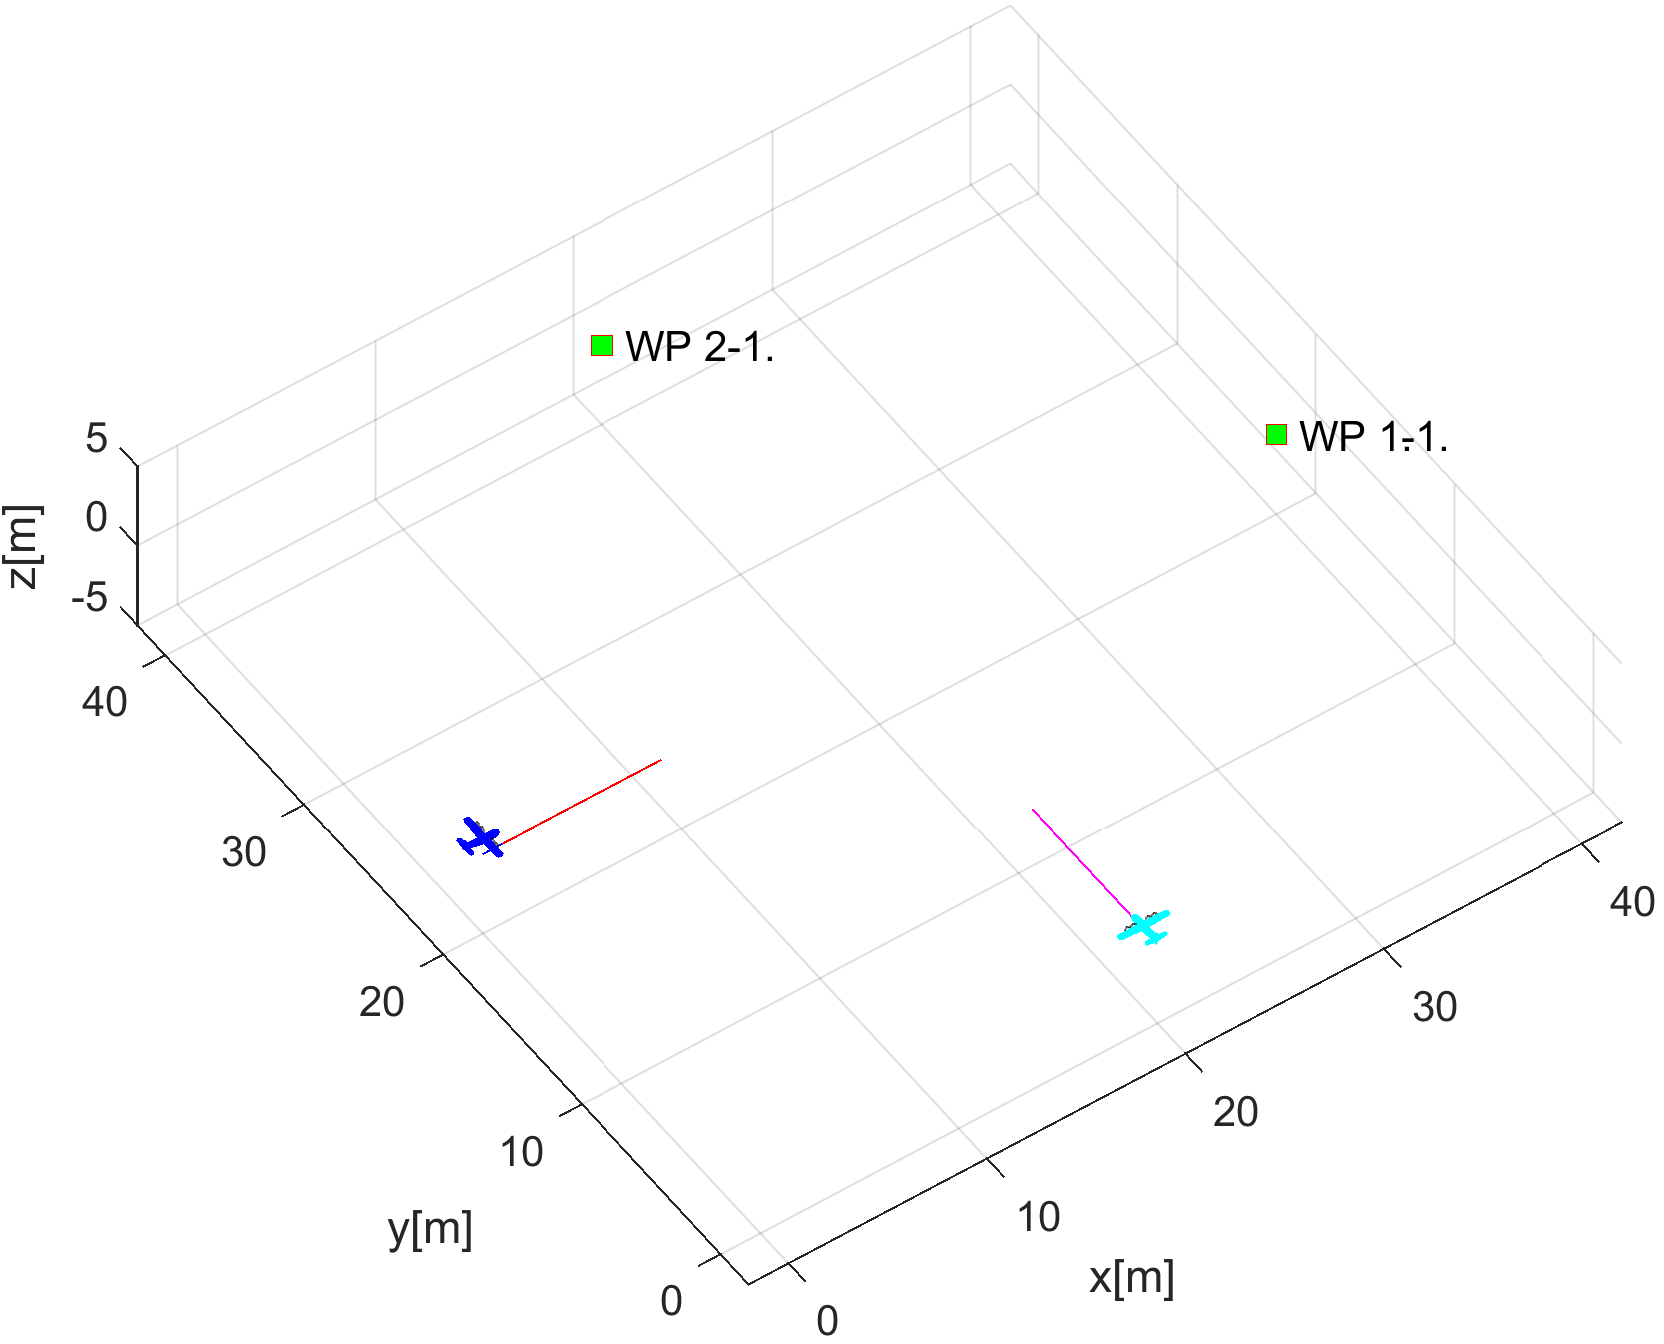
\includegraphics[width=0.9\linewidth]{\FIGDIR/NS025UtmEmergencyConverging00001}
        \caption{Situation detection.}
        \label{fig:emergencyConvergingSituationDetection}
    \end{subfigure}
    \begin{subfigure}{0.48\textwidth}
    	\centering
        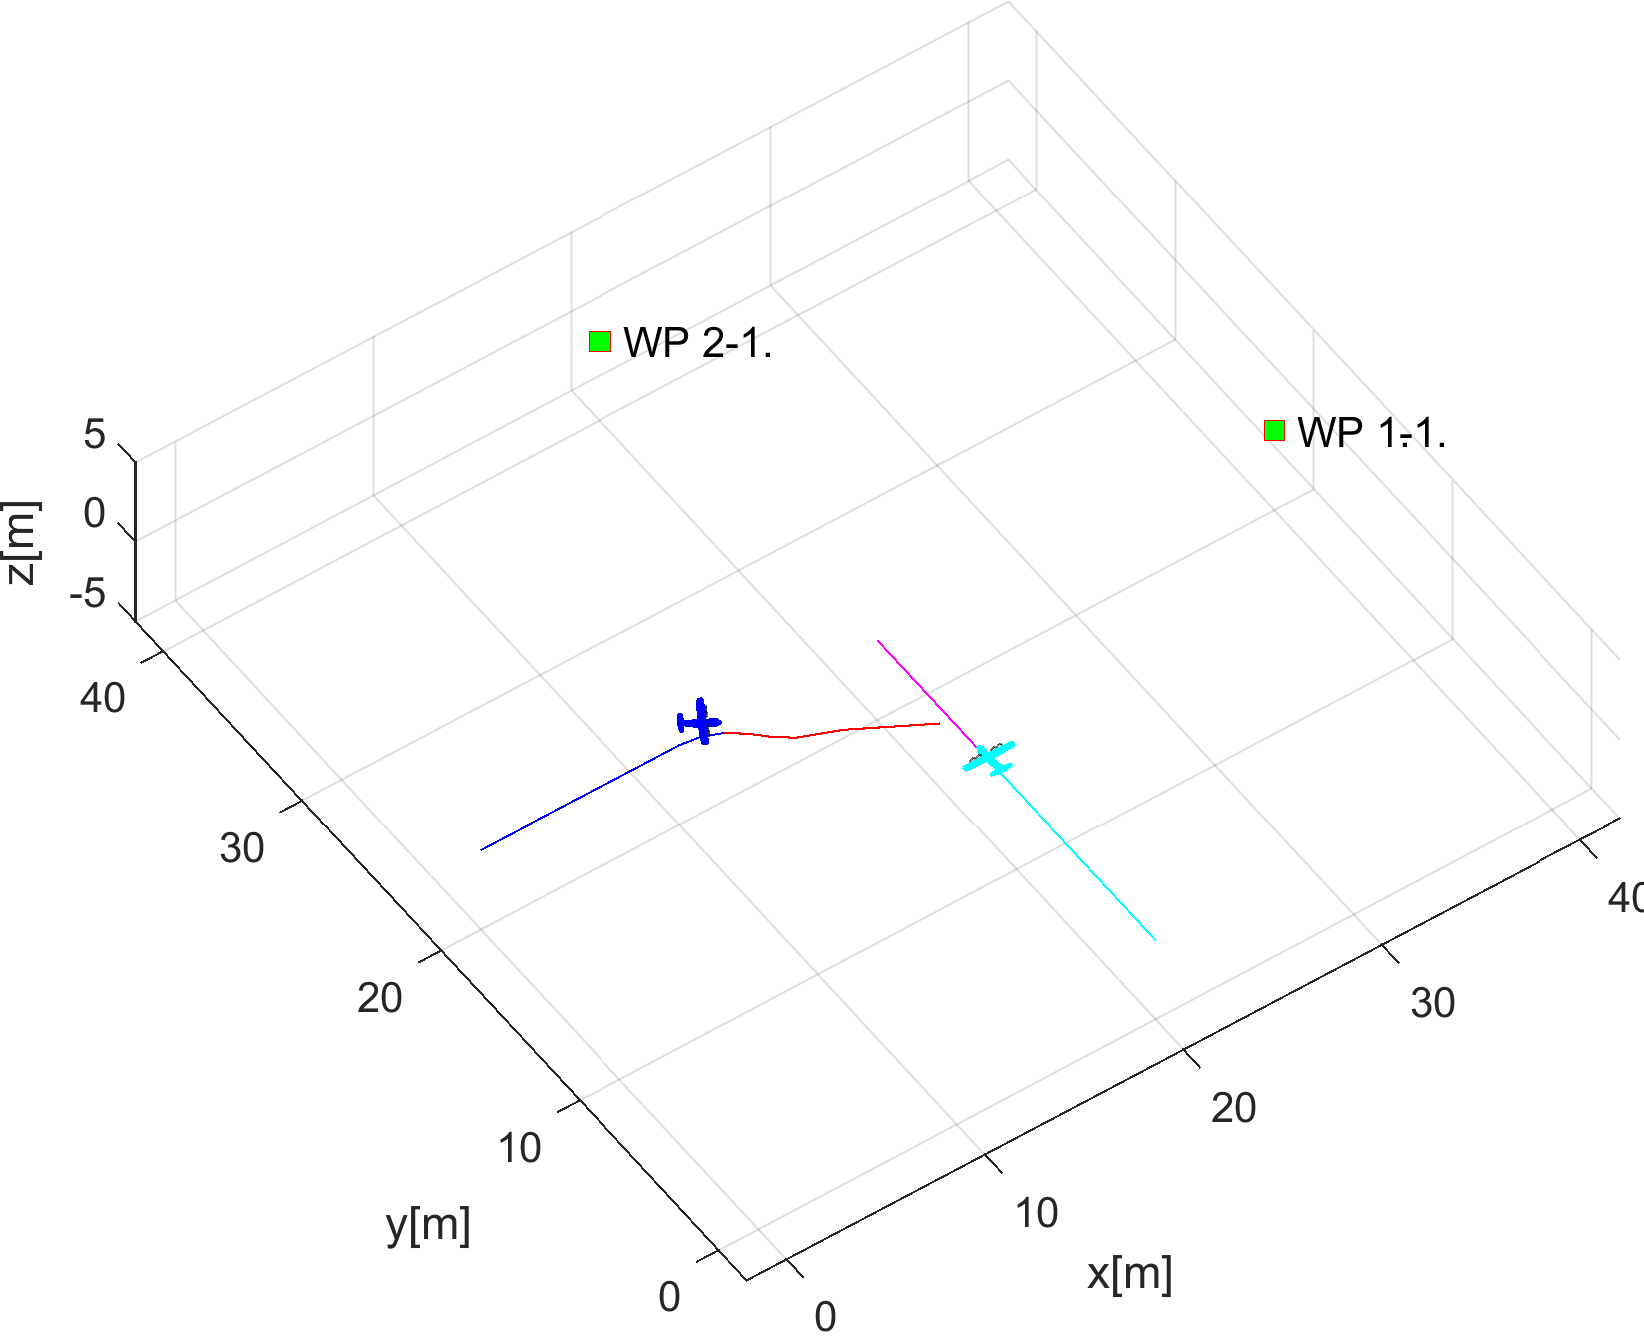
\includegraphics[width=0.9\linewidth]{\FIGDIR/NS026UtmEmergencyConverging00012} 
        \caption{Start converging.}
        \label{fig:emergencyConvergingStart}
    \end{subfigure}
    \\
    \begin{subfigure}{0.48\textwidth}
    	\centering
        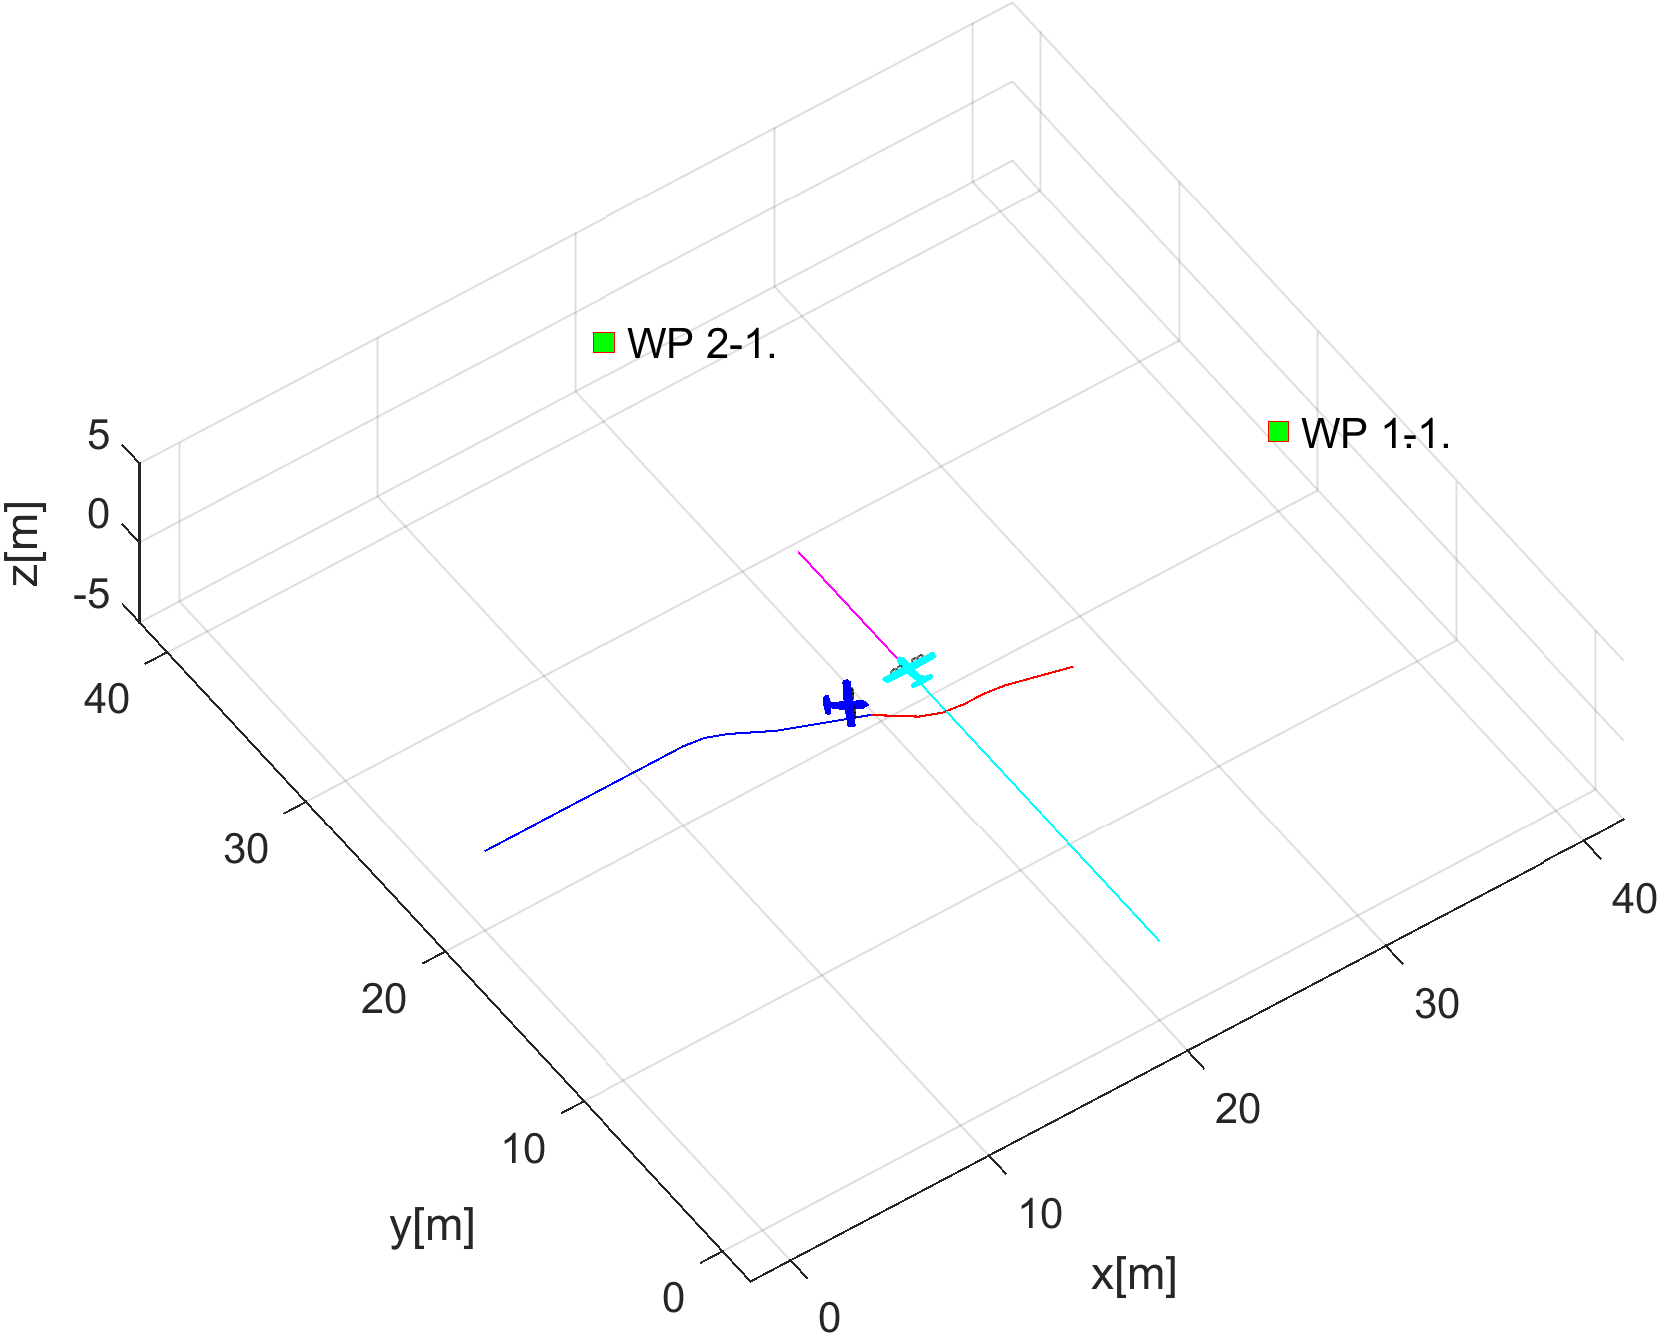
\includegraphics[width=0.9\linewidth]{\FIGDIR/NS027UtmEmergencyConverging00018} 
        \caption{Near miss case.}
        \label{fig:emergencyConvergingEnd}
    \end{subfigure}
    \begin{subfigure}{0.48\textwidth}
    	\centering
        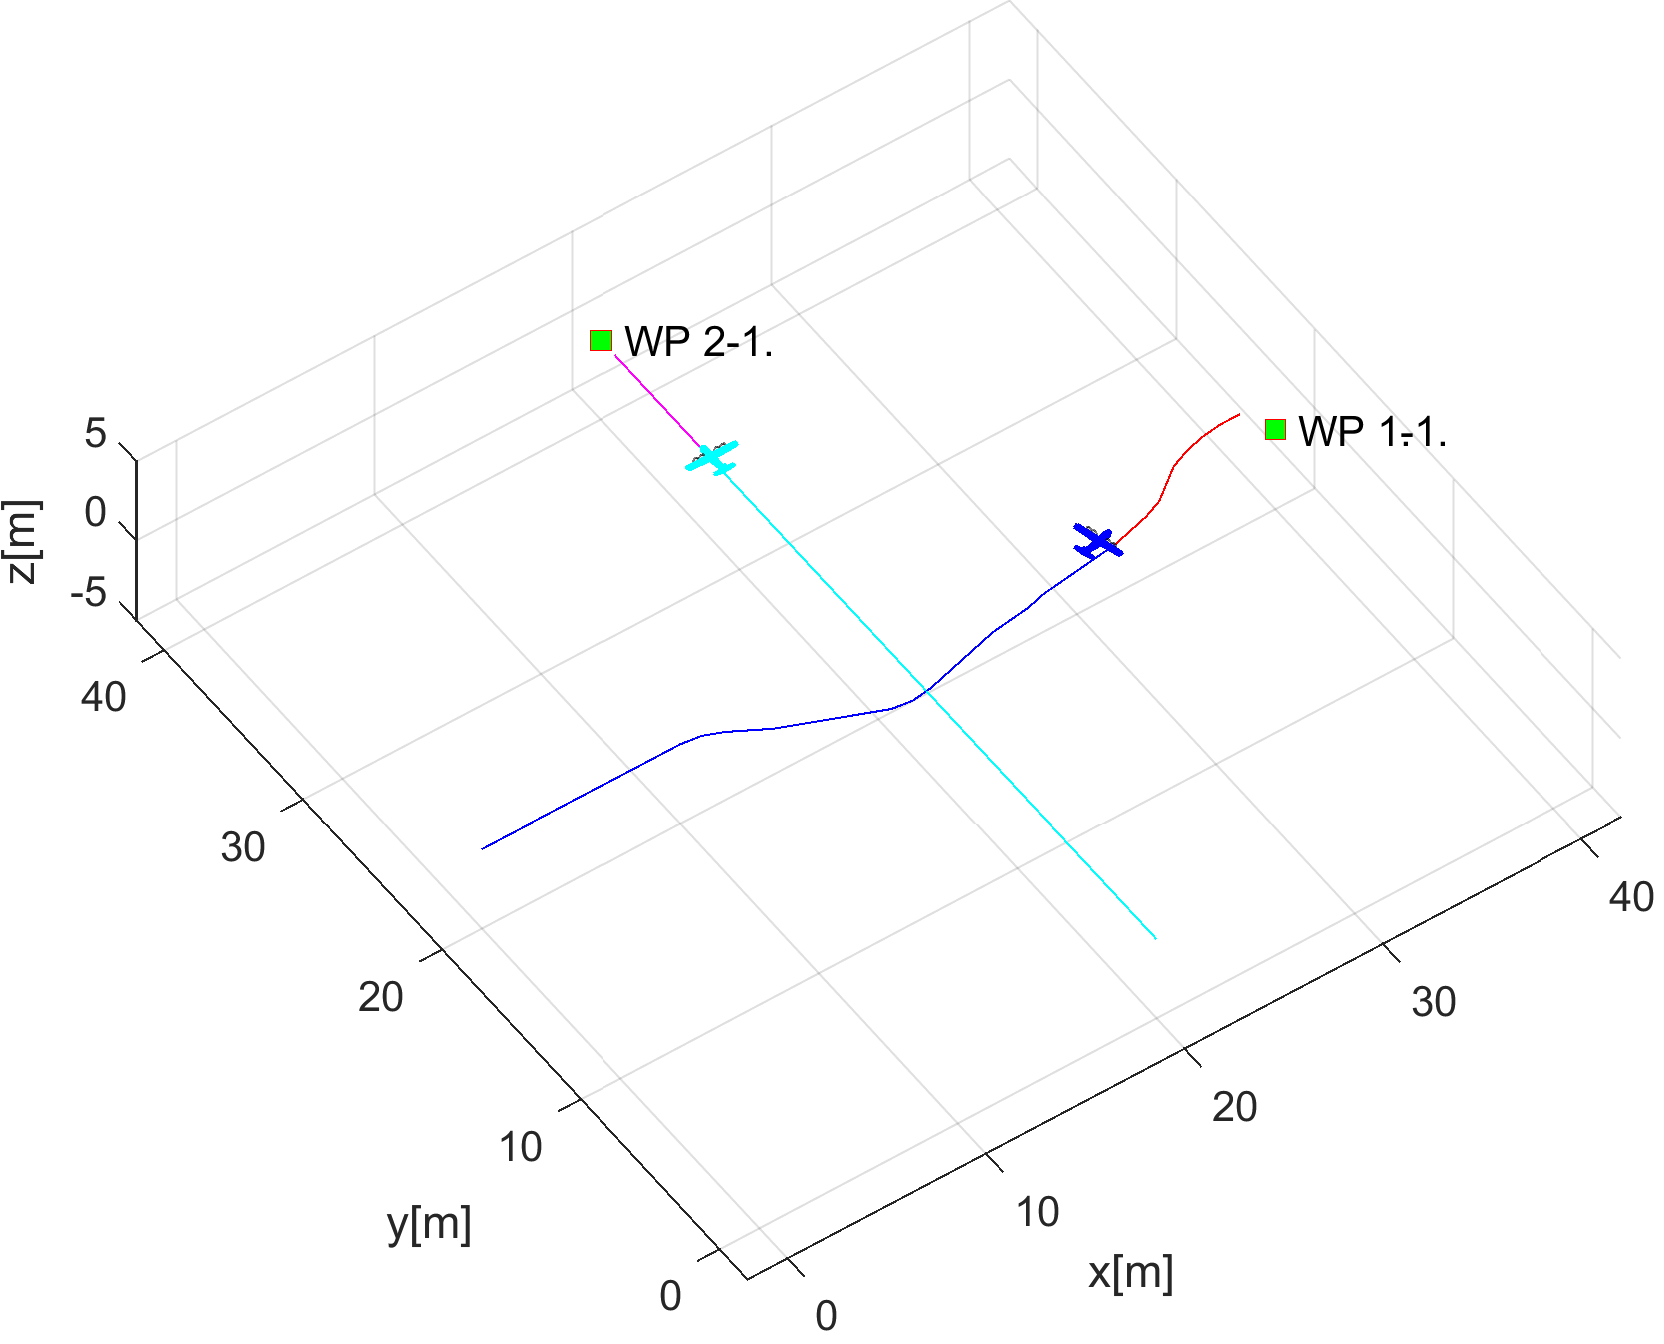
\includegraphics[width=0.9\linewidth]{\FIGDIR/NS028UtmEmergencyConverging00032} 
        \caption{Waypoints reach.}
        \label{fig:emergencyConvergingWaypointReach}
    \end{subfigure}
    \caption{Test scenario for \emph{Emergency converging} (Intruder avoidance). }
    \label{fig:testCaseEmergencyConverging}
\end{figure}

\begin{figure}[H]
    \centering
    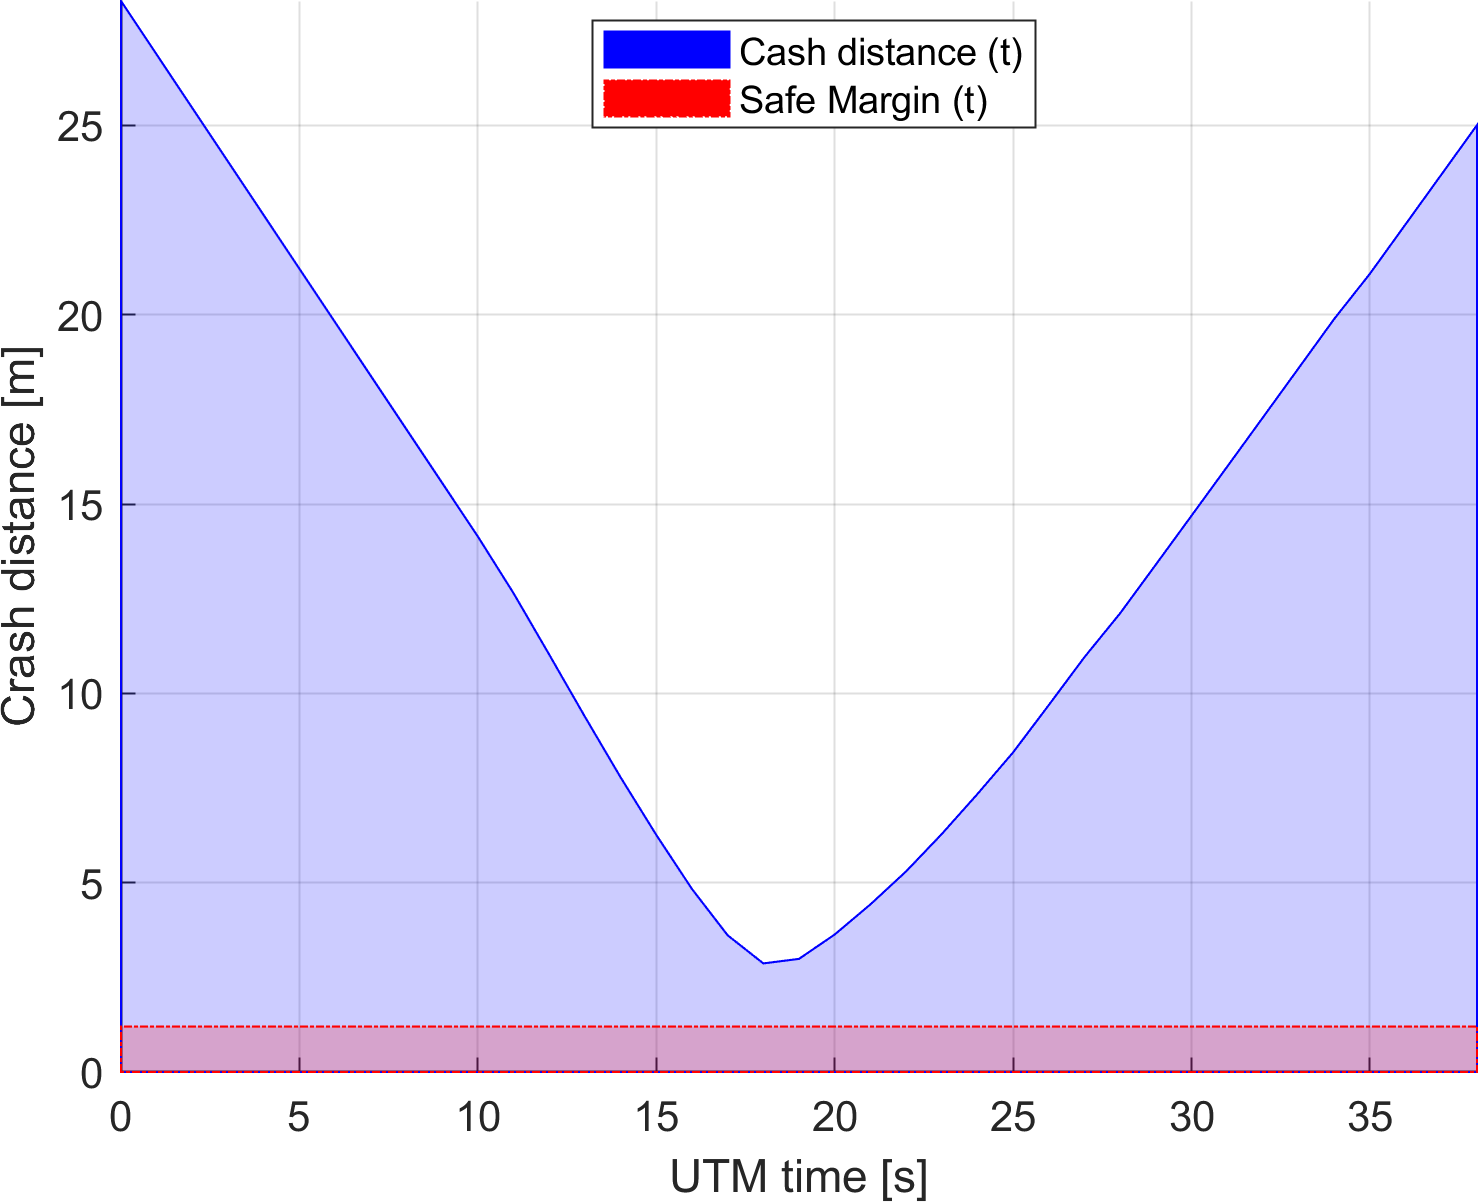
\includegraphics[width=0.55\linewidth]{\FIGDIR/NS029UtmEmergencyConvergingPerformance} 
    \caption{Distance to safety margin evolution for \emph{emergency converging scenario}.}
    \label{fig:testCaseEmergencyConvergingAvoidancePerformance}
\end{figure}

\paragraph{Distance to Safety Margin Evolution:} There is a need to compare the mutual distance between both UAS (y-axis [m]) and its evolution over UTM time (x-axis [s]). The \emph{mutual} distance of \emph{UAS 1} to \emph{UAS 2} is given by \emph{blue line}. The \emph{Safety margin} value is denoted by the red line at a  \emph{constant value} of $1.2$ $m$.

The \emph{Proper avoidance Invocation} is shown when UAS systems are getting closer to each other, and they enter (Emergency Avoidance Mode) to provide \emph{active separation}. The \emph{Mutual distance evolution} (blue line) does not cross \emph{safety margin} (red line).


\paragraph{Distance to Safety Margin Peaks:} Minimal and Maximal mutual distance to safety margin is summarized in (tab. \ref{tab:testCaseEmergencyConvergingSafetyMarginDistances}). The closest to the collision are UAS systems when the distance to safety margin is $1.6676m$.

The \emph{minimal distance to safety margin  $\ge$ 0} which means that the \emph{safety acceptance criterion} is fulfilled. 

\begin{table}[H]
    \centering
    \begin{tabular}{c|c||c}
    \multicolumn{2}{c||}{UAS:} & 1-2 \\\hline\hline
    \multirow{2}{*}{Distance to Safety Margin} & min & 1.6676 \\\cline{2-3}
                                            & max & 27.0843 \\
    \end{tabular}
    \caption{Distance to safety margin peaks for the \emph{emergency converging scenario}.}
    \label{tab:testCaseEmergencyConvergingSafetyMarginDistances}
\end{table}

\paragraph{Path Tracking Performance:} All waypoints (green numbered squares) for both  UAS have been reached (fig. \ref{fig:emergencyConvergingTrajectoryTrackingPerformance}). \emph{Reference trajectories} (green dashed lines), between the initial position (green square marked S) and goal waypoint (green square marked 1) are split into three XYZ values with respective figures. The tracked value is on y-axis [m] and time on x-axis [s]. The blue lines represent real parameter evolution over time.

Following observations can be made from path tracking (fig. \ref{fig:emergencyConvergingTrajectoryTrackingPerformance}) and preferred separations (tab. \ref{tab:aboidanceParametersForEmergencyConvergingScenario}):

\begin{enumerate}
    \item UAS 1 (fig. \ref{fig:emergencyConvergingUAS1PathTracking}) is using \emph{horizontal separation} (y-axis). The UAS diverges from the reference trajectory to minimum necessary time.
    
    \item UAS 2 (fig. \ref{fig:emergencyCovnergingUAS2PathTracking}) has the right of way and is not using any active avoidance mechanism. 
\end{enumerate}

\begin{figure}[H]
    \centering
    \begin{subfigure}{0.48\textwidth}
    	\centering
        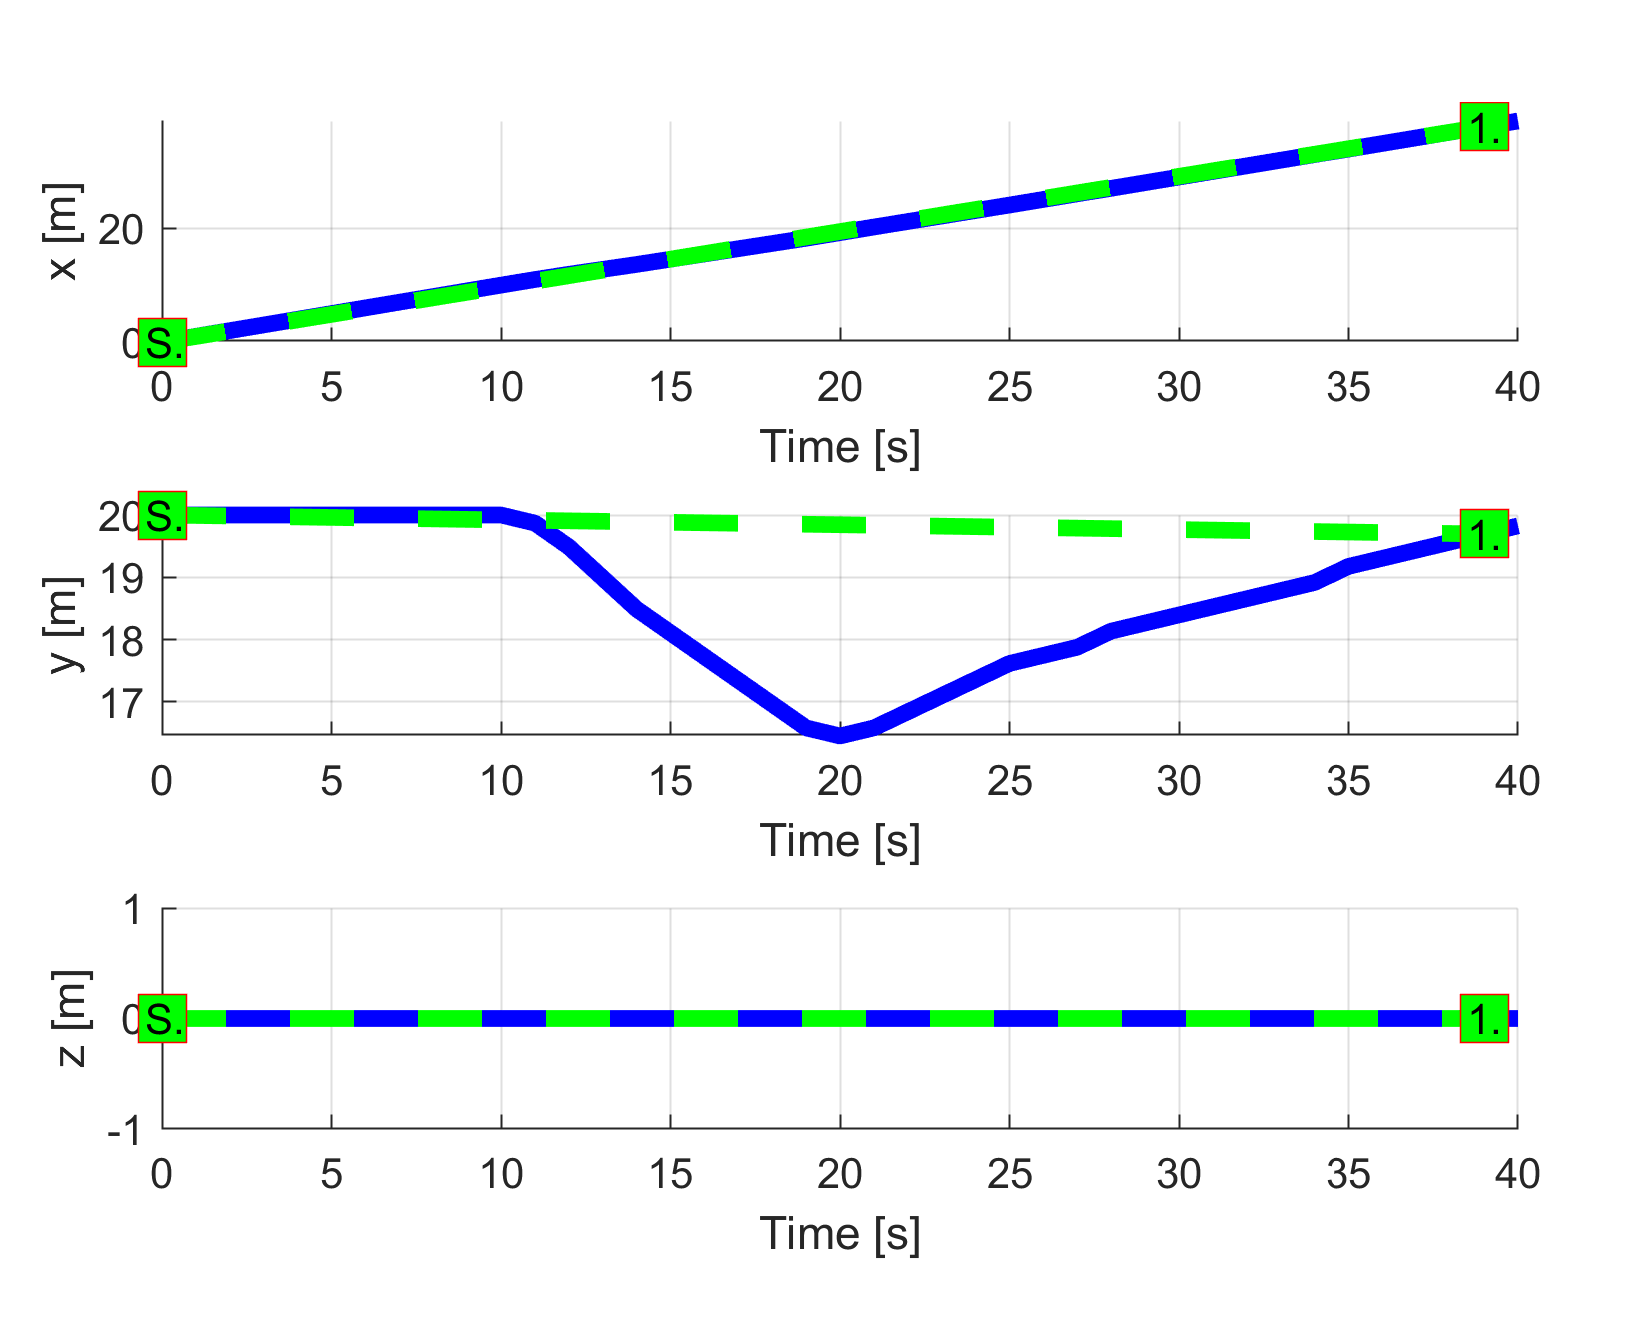
\includegraphics[width=0.9\linewidth]{\FIGDIR/NS030UtmEmergencyConvergingUAV1PathFollowing}
        \caption{UAS 1.}
        \label{fig:emergencyConvergingUAS1PathTracking}
    \end{subfigure}
    \begin{subfigure}{0.48\textwidth}
	    \centering
        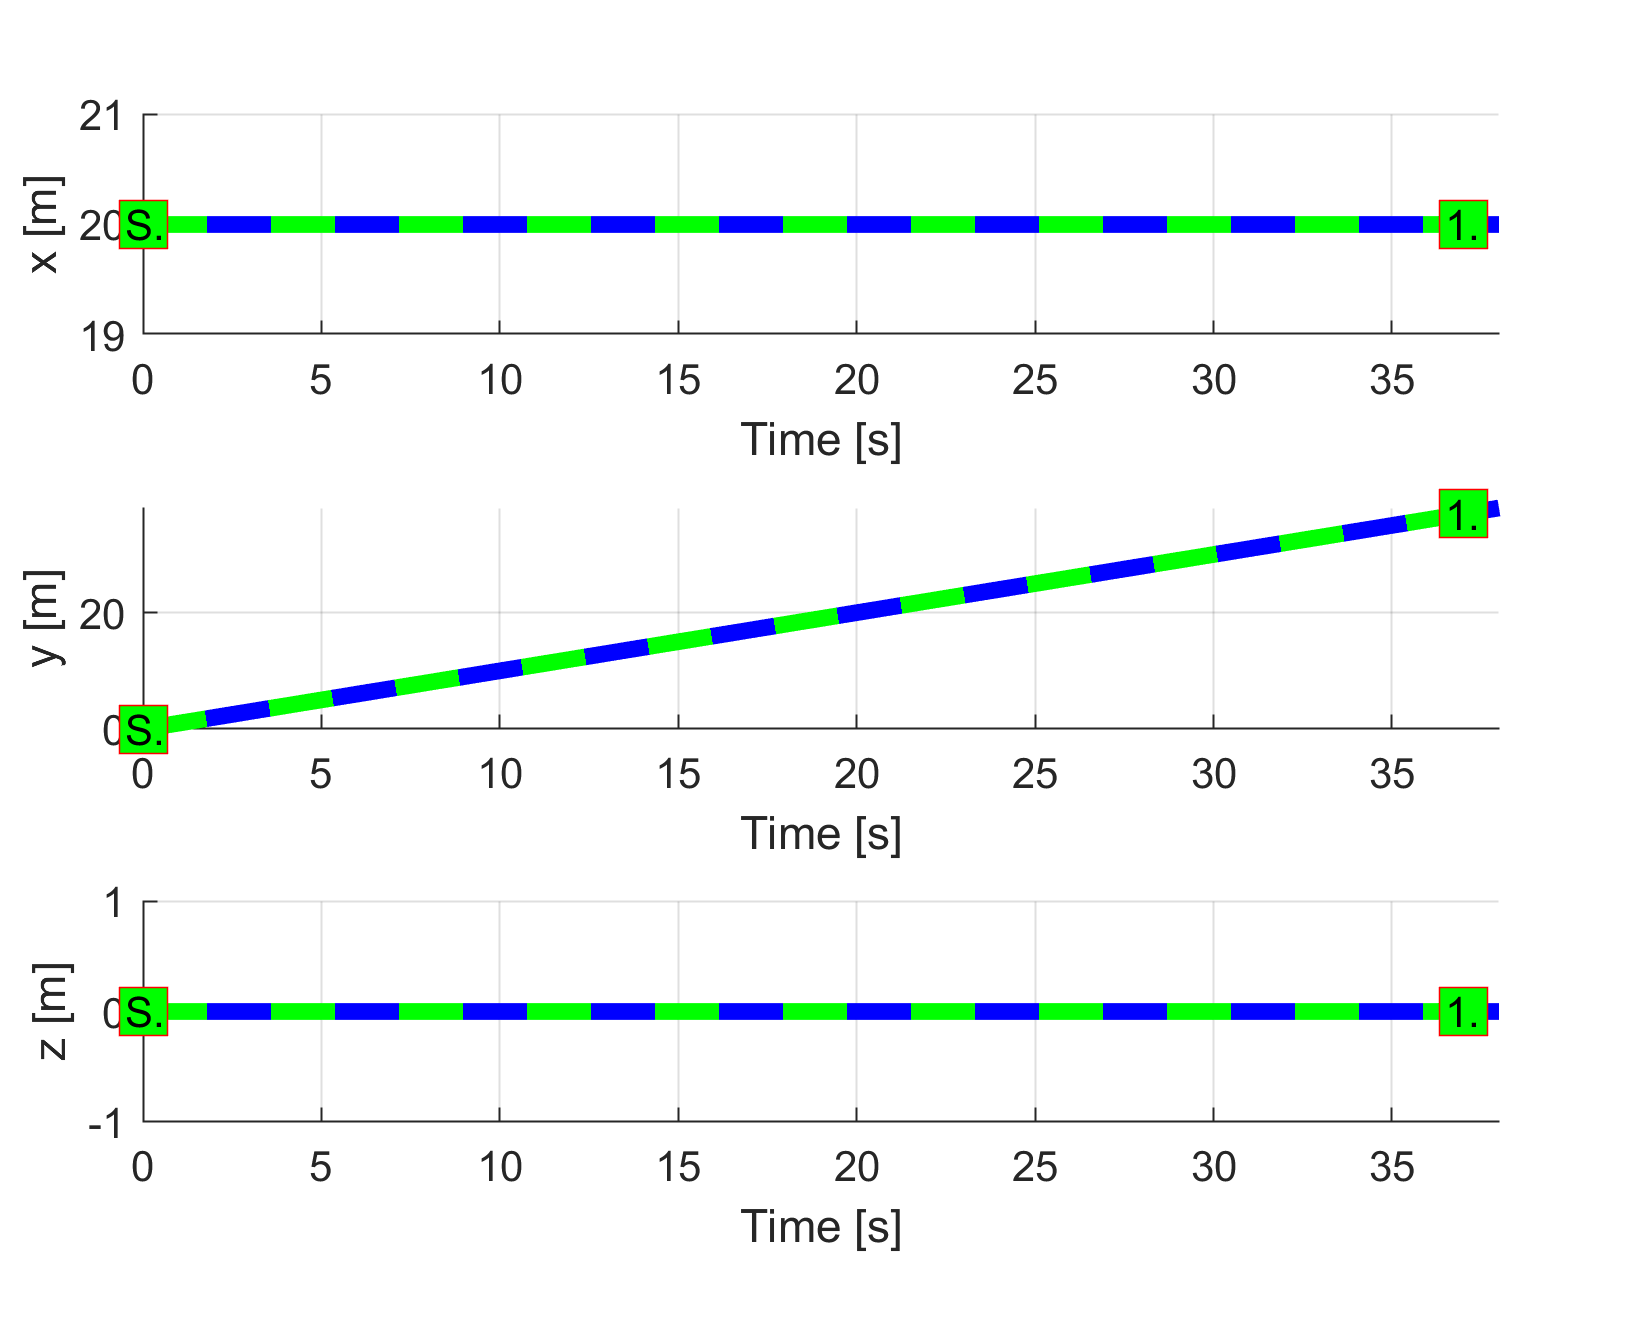
\includegraphics[width=0.9\linewidth]{\FIGDIR/NS031UtmEmergencyConvergingUAV2PathFollowing} 
        \caption{UAS 2.}
        \label{fig:emergencyCovnergingUAS2PathTracking}
    \end{subfigure}
    \caption{\emph{Trajectory tracking} for \emph{Emergency converging} test case. }
    \label{fig:emergencyConvergingTrajectoryTrackingPerformance}
\end{figure}

\paragraph{Path Following Deviations:} \emph{Deviations} (tab. \ref{tab:pathTrackingParametersForEmergencyConverging}) are in expected ranges considering the  \emph{mission plans} (tab. \ref{tab:missionSetupEmergencyConvergingScenario}) and \emph{separation safety margin} (tab. \ref{tab:aboidanceParametersForEmergencyConvergingScenario}).
    
\begin{table}[H]
    \centering
    \begin{tabular}{c||c|c}
        \multirow{2}{*}{Param.} & UAS 1     & UAS 2\\\cline{2-3}
                        & $\mathscr{WP}_1$  & $\mathscr{WP}_1$\\\hline\hline
          $\max |x|$    & 0                 & 0 \\\hline
          $\max |y|$    & 3.25              & 0 \\\hline
          $\max |z|$    & 0                 & 0 \\\hline
          $\max dist.$  & 3.25              & 0 \\
    \end{tabular}
    \caption{Path tracking properties for the\emph{Emergency converging} scenario.}
    \label{tab:pathTrackingParametersForEmergencyConverging}
\end{table}

% 05 Emergency Converging
\paragraph{Computation Load:} The \emph{computation load} for \emph{scenario} (fig.\ref{fig:emergencyConvergingComputationTime}) shows used time (y-axis) over decision frame (x-axis).

The \emph{computation time} is increased only for UAS 1 during the avoidance period. The UAS 2 remains unaffected because it has the right of way.

\begin{figure}[H]
    \centering
    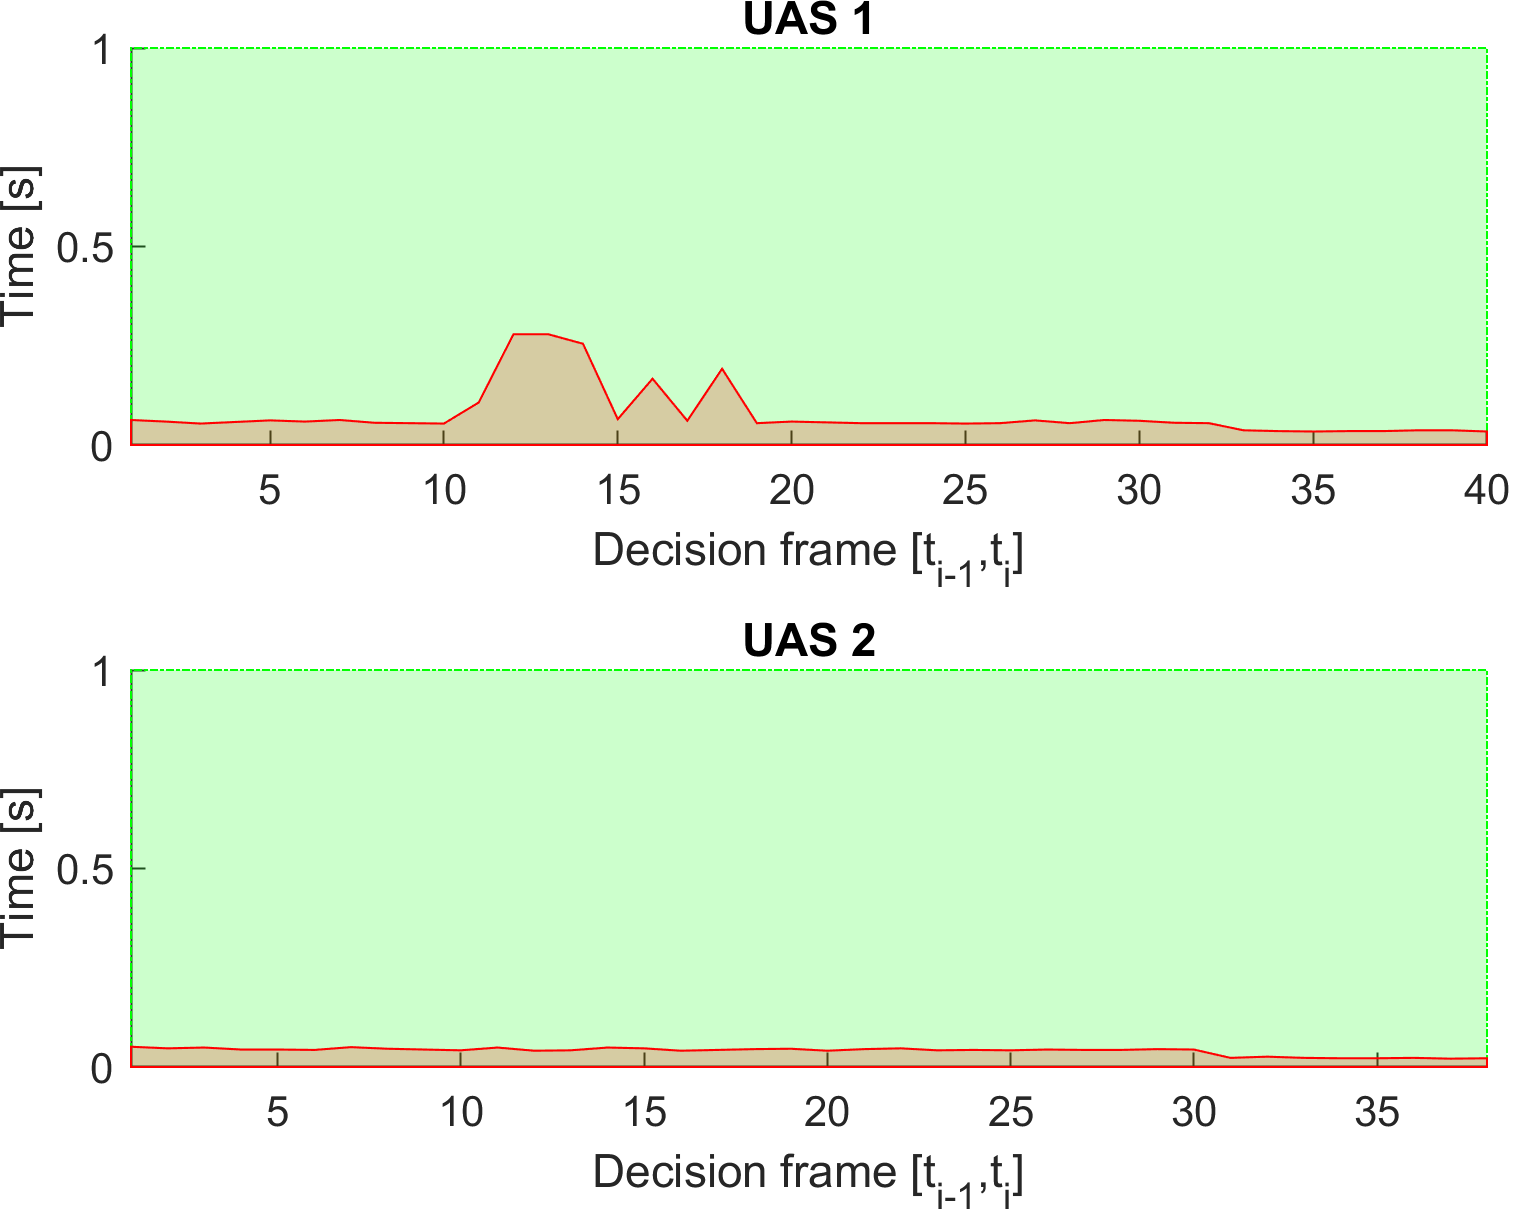
\includegraphics[width=0.65\linewidth]{\FIGDIR/NS096EmergencyConvergingComputationTime} 
    \caption{Computation time for \emph{Emergency converging} scenario.}
    \label{fig:emergencyConvergingComputationTime}
\end{figure}


    	\subsection{Emergency Head on}\label{s:testEmergencyHeadOn}

\paragraph{Scenario:} Two  \emph{UAS} systems are flying in an \emph{uncontrolled airspace} (altitude $\le$ 500 ft. Above the Ground Level) with missions defined in (tab. \ref{tab:missionSetupEmergencyHeadOnScenario}). Both \emph{UAS} are in the  \emph{Navigation mode} with active \emph{ADSB-In/Out}, receiving position notifications from each other. Cruising altitude is sufficient for horizontal separation (50-100 ft. Above Ground Level). \emph{Horizontal separation} is preferred mode for both \emph{UAS}.


\begin{table}[H]
    \centering
    \begin{tabular}{c||c|c||c}
        \multirow{2}{*}{UAS} &\multicolumn{2}{c||}{Position} & \multirow{2}{*}{$\mathscr{WP}_1$} \\\cline{2-3}
          & $[x,y,z]$           & $[\theta,\varpi,\psi]$           & \\\hline\hline
        1 & $[0,20,0]^T $       & $[0^\circ,0^\circ,0^\circ]^T$    & $[40,20,0]^T$\\\hline 
        2 & $[40,20,0]^T $       & $[0^\circ,0^\circ,180^\circ]^T$  & $[0,20,0]^T$\\ 
    \end{tabular}
    \caption{Mission setup for \emph{Emergency head on} scenario.}
    \label{tab:missionSetupEmergencyHeadOnScenario}
\end{table}


\begin{note}
\emph{Collision point} is expected at $\mathscr{C}=[20,20,0]^T$. The \emph{angle of approach} is $180^{\circ}$  which classifies situation as \emph{Head on maneuver} (fig. \ref{fig:HeadOnApproachTheoretical}).
\end{note}


\paragraph{Main Goal:} Show two \emph{non-cooperative } UAS avoidance for \emph{Head-on approach scenario} in \emph{uncontrolled} airspace.


\paragraph{Acceptance criteria:} 
\begin{enumerate}
    \item\emph{Proper mode invocation} - when an intruder intersects the opposing \emph{UAS} Navigation grid, bot intruder and \emph{UAS} will switch to \emph{Emergency Avoidance Mode}. None of the \emph{UAS} have \emph{Right Of the Way}.
    
    \item\emph{Minimal Safety Margin distance} $\ge 0m$. That means the mutual distance of both \emph{UAS centers} does not go below given \emph{safety margin}.
    
    \item\emph{Both UAS} will reach own goal waypoint (tab. \ref{tab:missionSetupEmergencyHeadOnScenario}).

\end{enumerate}

\paragraph{Testing setup:} The \emph{standard test setup} for each UAS defined in (tab \ref{tab:testMovementOrientations}, \ref{tab:testUASBasicParameters}, \ref{tab:testNavigationGridBasic}, \ref{tab:testAvoidanceGridBasic}, \ref{tab:testUASColoring}) is used with following without parameter override.

\emph{Intruder intersection} model has been chosen depending on UAS (tab. \ref{tab:aboidanceParametersForEmergencyHeadOnScenario}). Each UAS is equipped with \emph{ADS-B In/Out} sensor obtaining/distributing following information:

\begin{enumerate}
    \item \emph{Position} - in operational section coordinate frame.
    
    \item \emph{Velocity} - vector representation in given coordinate frame.
    
    \item \emph{Class size} - class body radius based on UAS propulsion and size.
    
    \item \emph{Safety margin set} - set of safety margins for different collision cases.
\end{enumerate}

\noindent \emph{Avoidance parameters} for \emph{Emergency head-on scenario} are given in (tab. \ref{tab:aboidanceParametersForEmergencyHeadOnScenario}). Each UAS has same speed set to $1 m s^{-1}$. None of them have the \emph{Right of The Way}. 

\emph{Safety margin} is considered as sum of both participants \emph{near miss margins}. In this case default safety margin is considered as $1.2$ $m$.

\begin{table}[H]
    \centering
    \begin{tabular}{c||c|c|c||c|c||c}
        \multirow{2}{*}{UAS} & \multicolumn{3}{c||}{Parameters} & \multicolumn{2}{c||}{Margins} & \multirow{2}{*}{Separation}                                            \\\cline{2-6}
                             & velocity & intruder model & ROW        & body & safety \\\hline\hline
        1                    & 1        & body (timed)  & false            & 0.3         & 0.6           & horizontal\\\hline
        2                    & 1        & body (timed)  & false             & 0.3         & 0.6  & horizontal          \\
    \end{tabular}
    \caption{Avoidance parameters for  \emph{Emergency head on} scenario.}
    \label{tab:aboidanceParametersForEmergencyHeadOnScenario}
\end{table}


\begin{note}
Both UAS are using  body (sec. \ref{s:bodyvolumeIntersection}) intersection model, reflecting both body volume along expected trajectory. Both UAS have preference for \emph{horizontal} separation mode, typical for planes.
\end{note}

\paragraph{Simulation Run:} Notable moments from the simulation run (fig. \ref{fig:testCaseEmergencyHeadOnApproach}) are following:

\begin{enumerate}
    \item \emph{Situation detection} (fig. \ref{fig:emergencyConvergingSituationDetection}) - UAS 1 (blue)  is approaching UAS 2 (cyan) with $130^\circ \le angle Of Approach \le 180^\circ$, this is considered head on approach. Head on approach  give the \emph{right of the way} neither to \emph{UAS 1} nor \emph{UAS 2}. \emph{Intruder intersection model} for opposite UAS is created in respective \emph{avoidance grids}. \emph{Head on emergency avoidance} starts independently in each UAS without intruders coordination. First \emph{avoidance maneuver} is invoked when the \emph{intruder intersection model} constraints any trajectory in the \emph{avoidance grid}. When this happens \emph{Navigation mode} switch to the \emph{Emergency avoidance mode}.
                
    \item \emph{Before near miss} (fig. \ref{fig:emergencyHeadOnBeforeNearMiss}) - both \emph{UAS} are in \emph{emergency avoidance mode}, sticking to right side avoidance maneuver.
    
    \item \emph{Near miss case} (fig. \ref{fig:emergencyHeadOnNearMiss}) - UAS 1 to UAS 2 closest distance. The safety margin for \emph{near miss} has not been breached. The safety margin for \emph{well clear} in uncontrolled airspace is invalid. Both UAS are using also \emph{Horizontal separation} to avoid each other, \emph{Emergency avoidance mode} is switched to the \emph{Navigation mode} when risk of an \emph{aerial clash} is voided.
    
    \item \emph{After near miss} (fig. \ref{fig:emergencyHeadOnAfterNearMiss}) - both \emph{UAS} are tracking back to respective waypoint, correcting \emph{altitude} (Z-axis in (fig. \ref{fig:emergencyHeadOnTrajectoryTrackingPerformance})) first.
    
    \item Note \emph{Collision point} was expected at $\mathscr{C}=[20,20,0]^T$
    
    \item Note \emph{Both UAS} used \emph{horizontal} (primary), \emph{vertical} (secondary) separation (fig \ref{fig:emergencyHeadOnTrajectoryTrackingPerformance}).
    
    \item Note \emph{Both UAS} decision times were \emph{synchronized}, this is not an assumption, but it shows critical performance. Usually safety margin is bloated for (eq.\ref{safetyMarginBloat}).
\end{enumerate}


\begin{figure}[H]
    \centering
    \begin{subfigure}{0.75\textwidth}
        \centering
        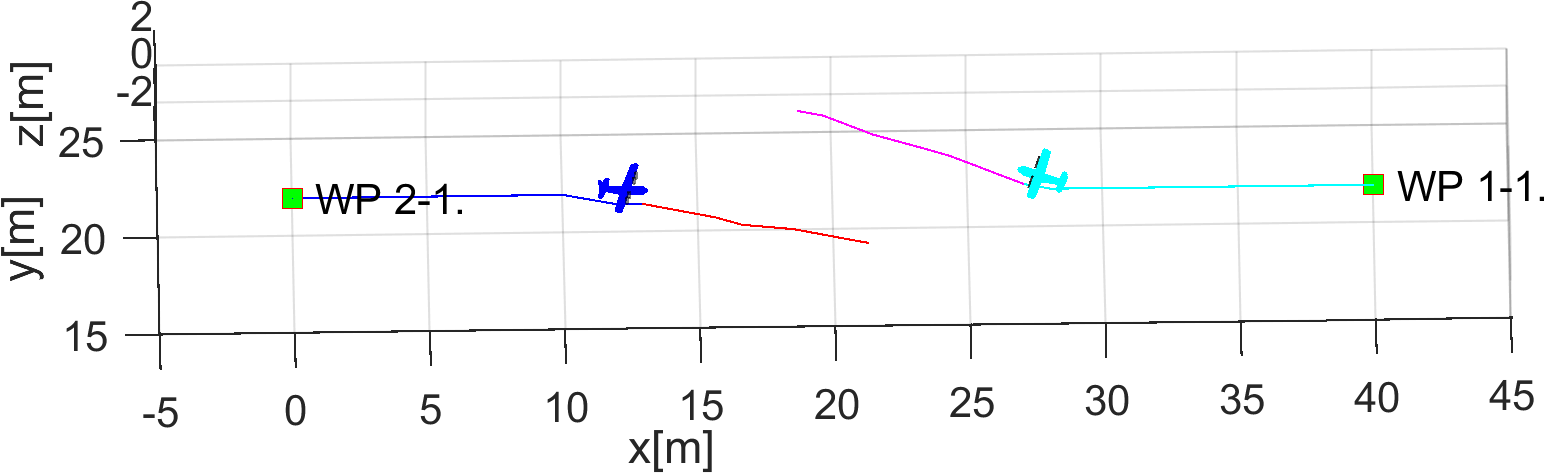
\includegraphics[width=0.9\linewidth]{\FIGDIR/NS032UtmEmergencyHeadOn00013}
        \caption{Situation detection.}
        \label{fig:emergencyHeadOnSituationDetection}
    \end{subfigure}
    \\
    \begin{subfigure}{0.75\textwidth}
        \centering
        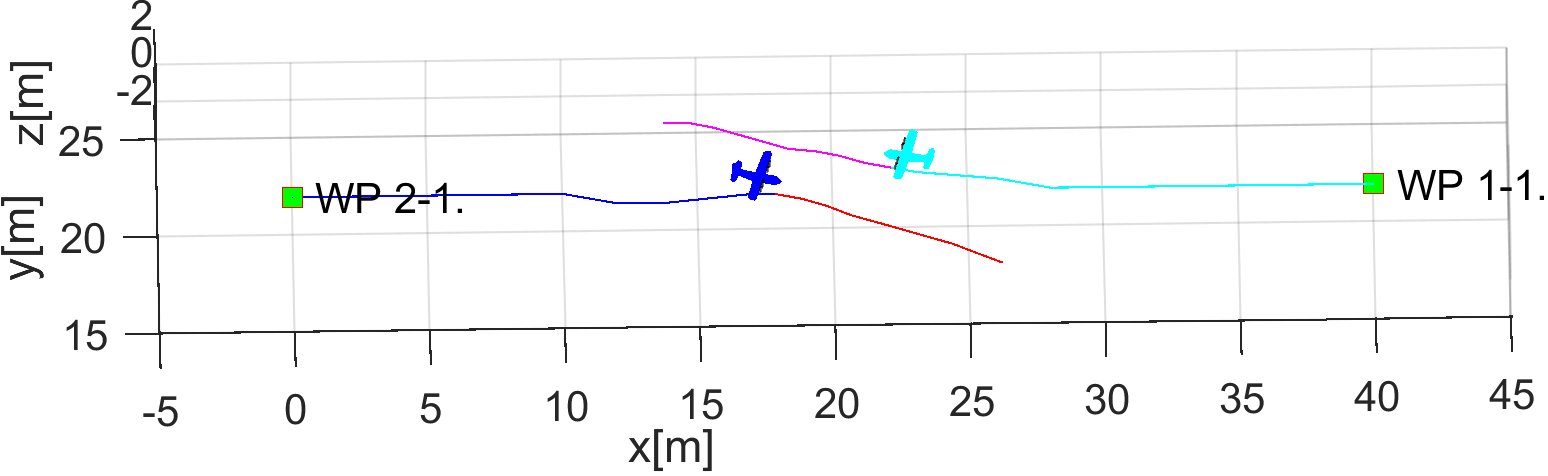
\includegraphics[width=0.9\linewidth]{\FIGDIR/NS033UtmEmergencyHeadOn00018} 
        \caption{Before near miss.}
        \label{fig:emergencyHeadOnBeforeNearMiss}
    \end{subfigure}
    \\
    \begin{subfigure}{0.75\textwidth}
        \centering
        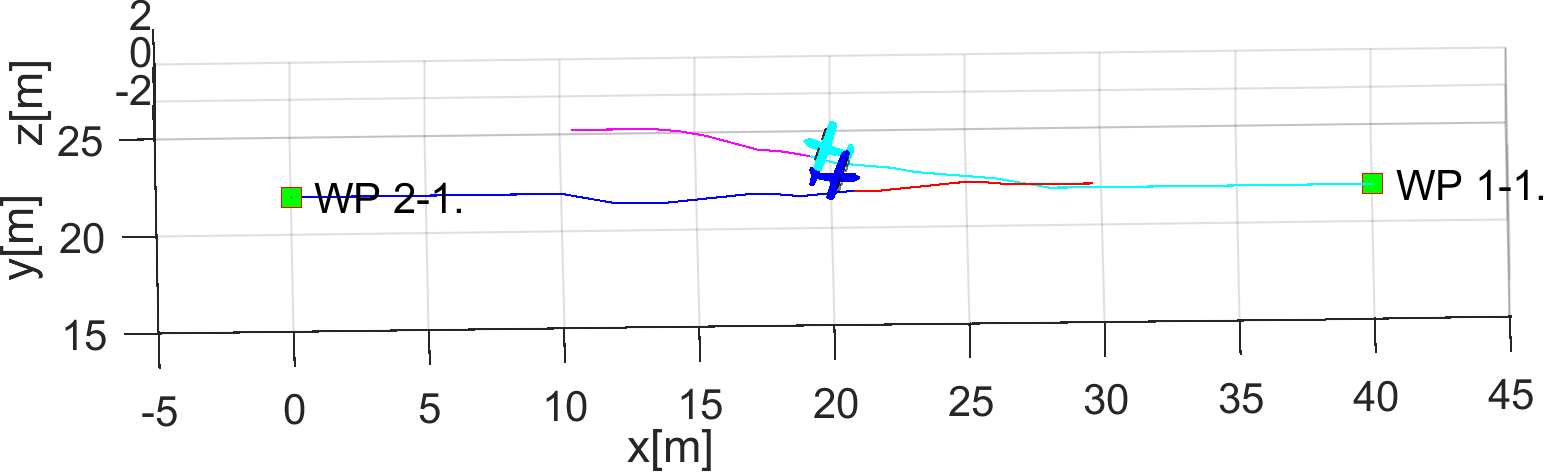
\includegraphics[width=0.9\linewidth]{\FIGDIR/NS034UtmEmergencyHeadOn00021} 
        \caption{Near miss.}
        \label{fig:emergencyHeadOnNearMiss}
    \end{subfigure}
    \\
    \begin{subfigure}{0.75\textwidth}
        \centering
        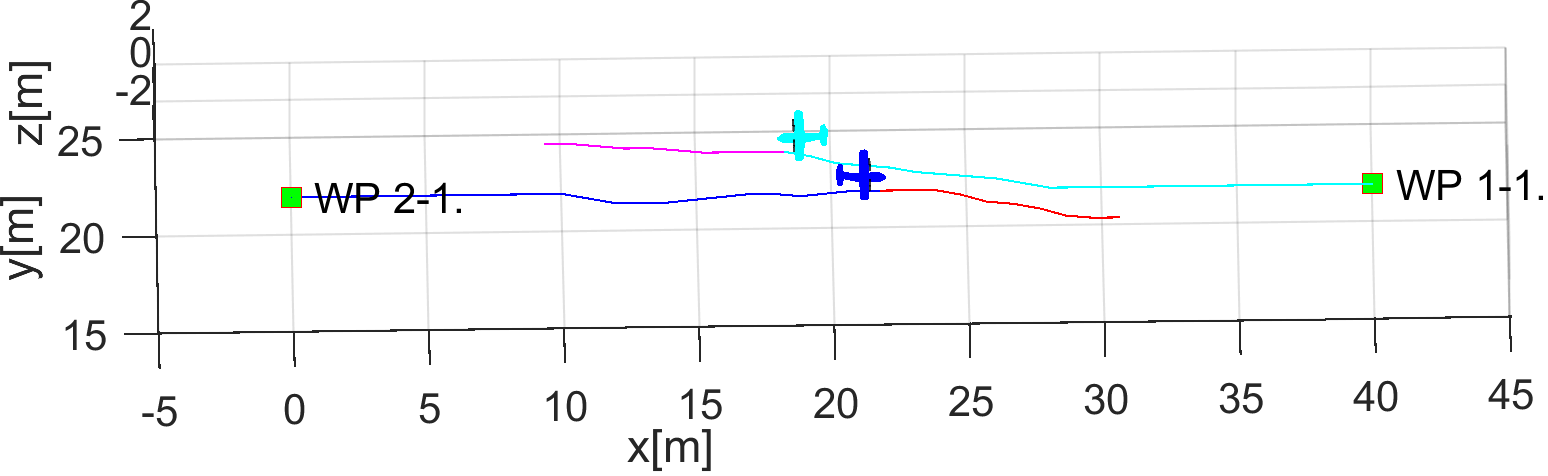
\includegraphics[width=0.9\linewidth]{\FIGDIR/NS035UtmEmergencyHeadOn00022} 
        \caption{After near miss.}
        \label{fig:emergencyHeadOnAfterNearMiss}
    \end{subfigure}
    \caption{Test scenario for \emph{Emergency head on approach} (Intruder avoidance). }
    \label{fig:testCaseEmergencyHeadOnApproach}
\end{figure}


\paragraph{Distance to Safety Margin Evolution:} There is need to compare mutual distance between both UAS (y-axis [m]) and its evolution over synchronized \emph{UTM time} (x-axis [s].) The \emph{mutual distance} between bodies of \emph{UAS 1}, \emph{UAS 2} (blue line) compared to \emph{Safety Margin} (red line) is given in (fig. \ref{fig:testCaseHeadOnAvoidancePerformance}). The \emph{Safety Margin} value was constant for all time at value $1.2$ $m$ which is double of \emph{Near Miss Margin for UAS 1 UAS 2}.

The proper \emph{Avoidance Invocation} is shown when \emph{UAS} systems are getting closer to each other and they starts their \emph{separation phase} (Emergency Avoidance Mode switch). The mutual distance (blue line) does not cross \emph{safety margin} (red line).

\begin{figure}[H]
    \centering
    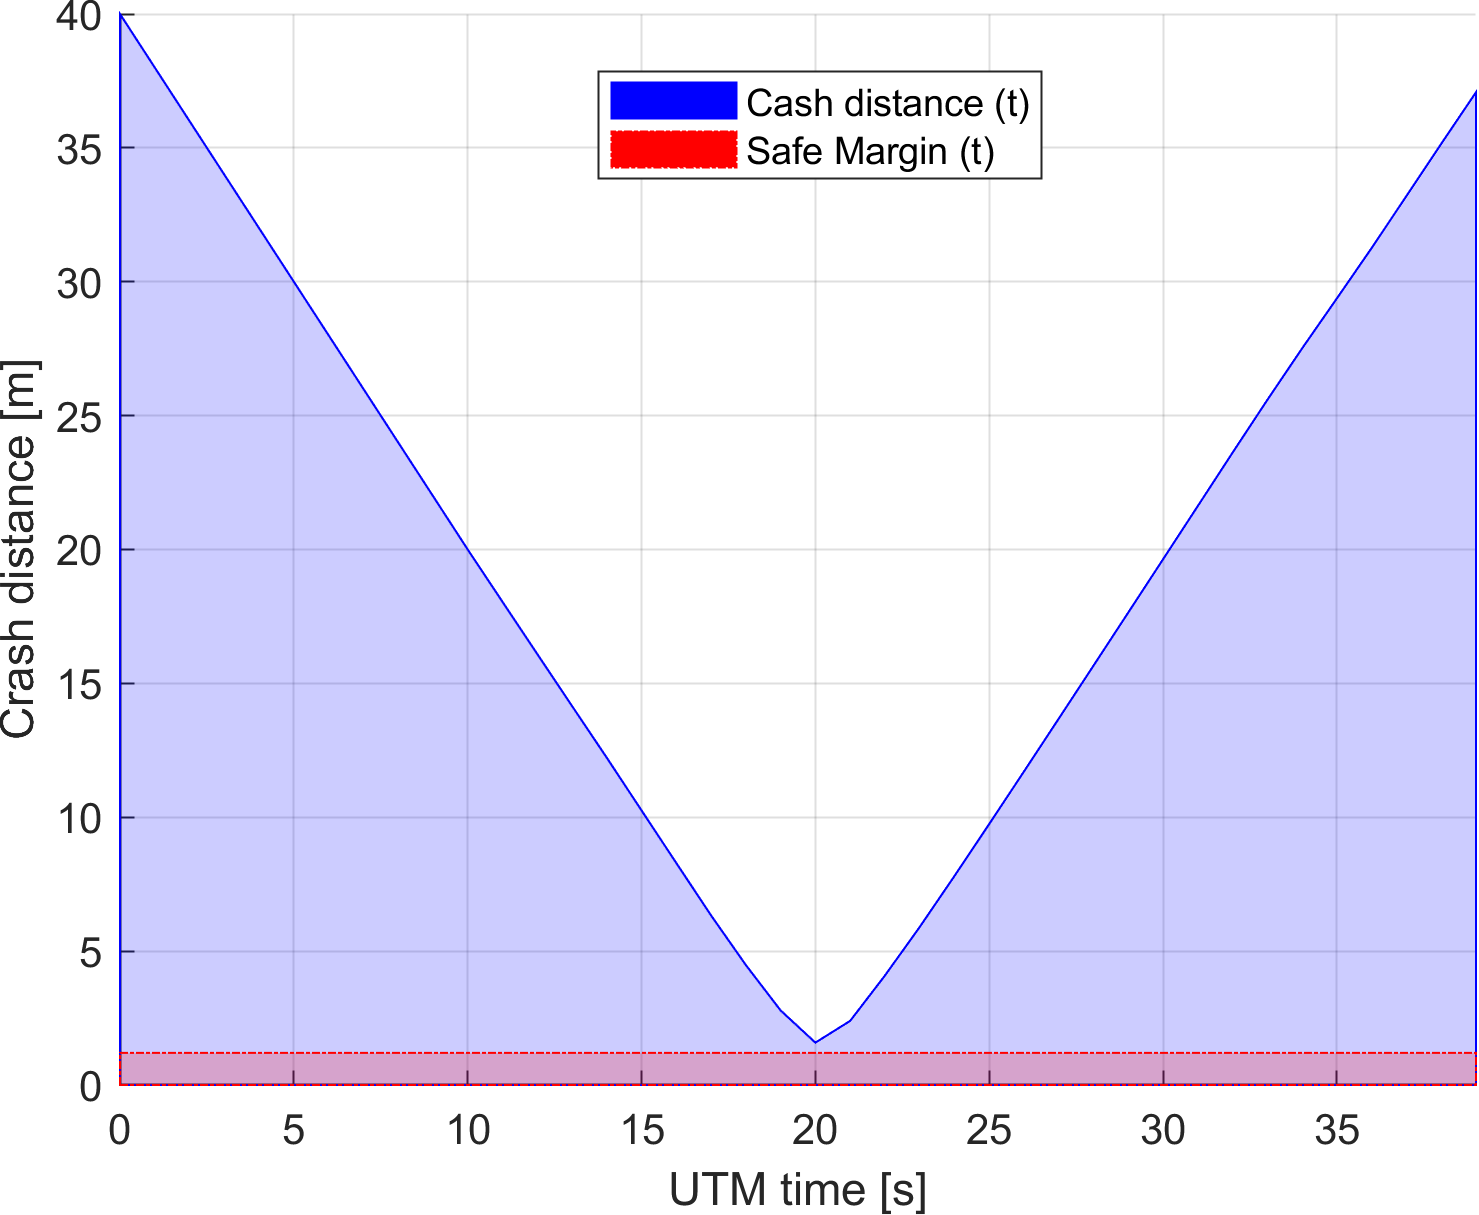
\includegraphics[width=0.55\linewidth]{\FIGDIR/NS036UtmEmergencyHeadOnPerformance} 
    \caption{Distance to safety margin evolution for \emph{emergency head on scenario}.}
    \label{fig:testCaseHeadOnAvoidancePerformance}
\end{figure}


\paragraph{Distance to Safety Margin Peaks:} Minimal and Maximal mutual distance to safety margin is summarized in (tab. \ref{tab:testCaseEmergencyHeadOnSafetyMarginDistances}). The closest to collision are UAS systems  when \emph{distance to safety margin} is $0.3824 m$.

The \emph{minimal distance to safety margin} $\ge$ $0$ which means that the \emph{safety acceptance criterion} is full filled.


\begin{table}[H]
    \centering
    \begin{tabular}{c|c||c}
    \multicolumn{2}{c||}{UAS:} & 1-2 \\\hline\hline
    \multirow{2}{*}{safety margin distance} & min & 0.3824 \\\cline{2-3}
                                            & max & 38.8000 \\
    \end{tabular}
    \caption{Distance to safety margin peaks for \emph{Emergency head on scenario}.}
    \label{tab:testCaseEmergencyHeadOnSafetyMarginDistances}
\end{table}

\paragraph{Path Tracking Performance} All waypoints (green numbered squares) for both UAS have been reached (fig. \ref{fig:emergencyHeadOnTrajectoryTrackingPerformance}). \emph{Reference trajectories} (green dashed lines), between initial position (green square marked S) and goal waypoint (green square marked 1) are split into three XYZ values with respective figures. The tracked value is on y-axis [m] and time on x-axis [s]. The blue lines represents real parameter evolution over time.

Following observations can be made from path tracking (fig.\ref{fig:emergencyHeadOnTrajectoryTrackingPerformance}) and preferred separations (tab. \ref{tab:aboidanceParametersForEmergencyHeadOnScenario}):

\begin{enumerate}
    \item UAS 1 (fig. \ref{fig:emergencyHeadOnUAS1PathTracking}) is using horizontal separation going to the right (y-axis) and a little bit up (z-axis).
    
    \item UAS 2 (fig. \ref{fig:emergencyHeadOnUAS2PathTracking}) is using horizontal separation going to the right (left in GCS, y-axis) and little bit up (z-axis).
\end{enumerate}

\begin{figure}[H]
	\centering
    \begin{subfigure}{0.48\textwidth}
    	\centering
        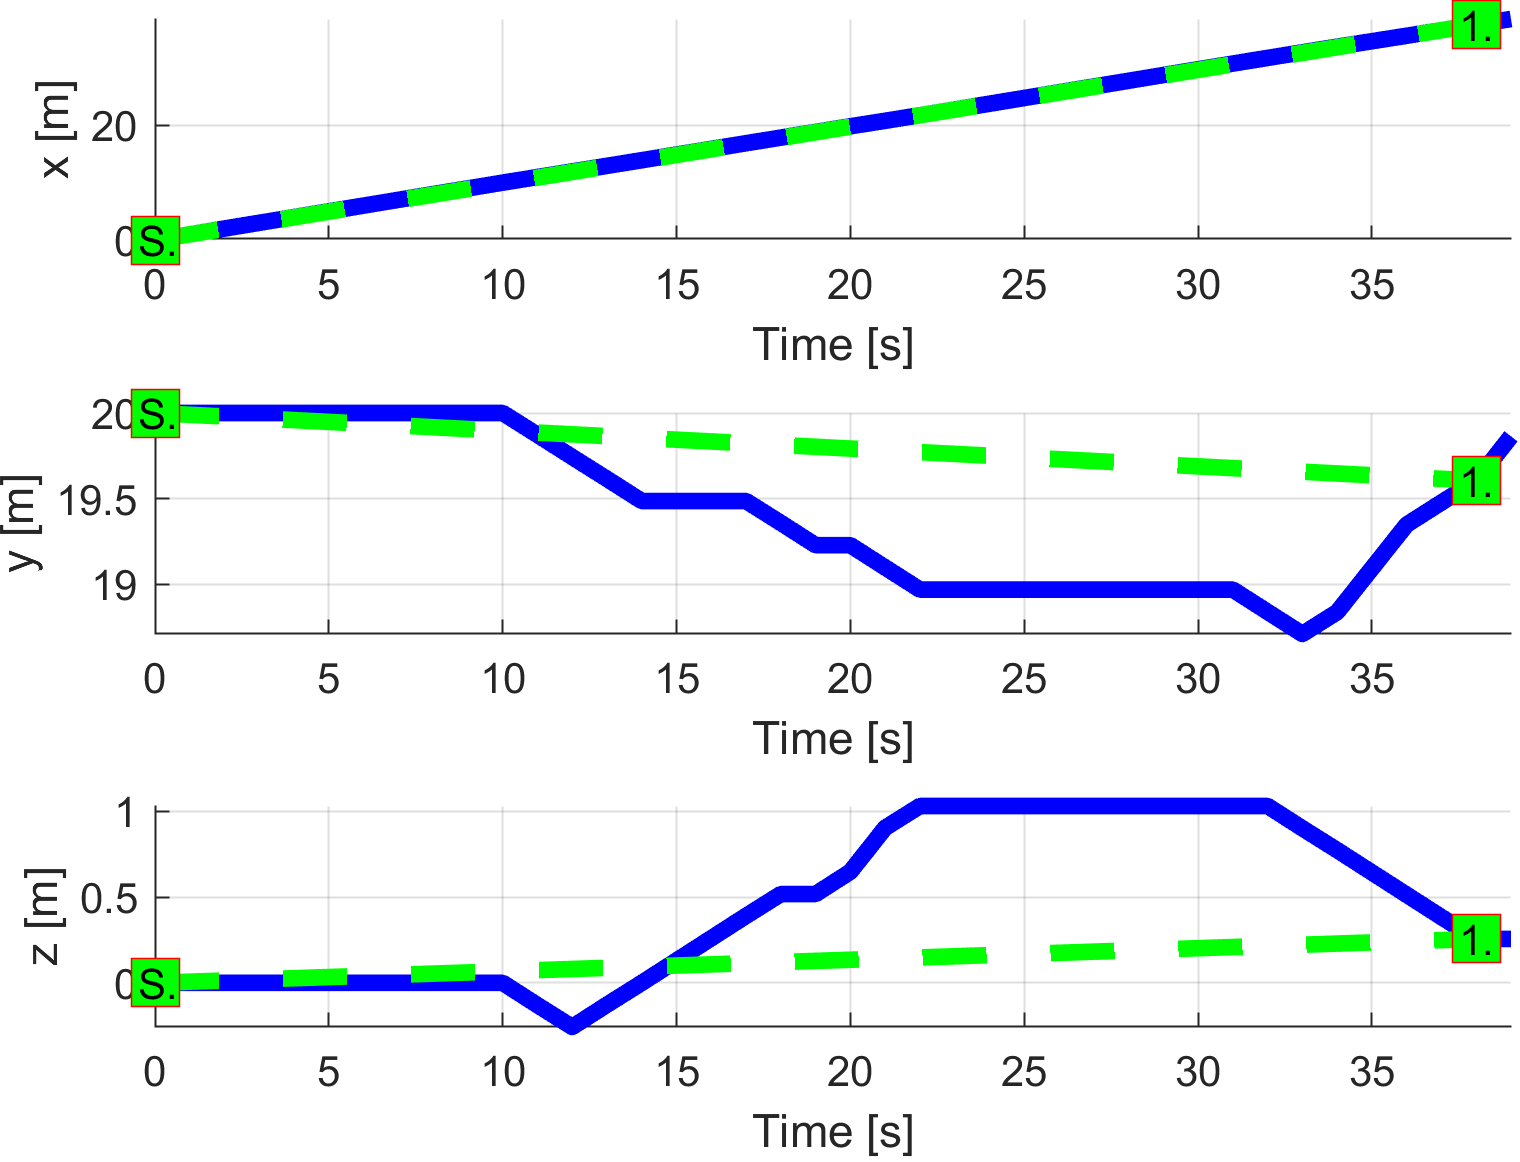
\includegraphics[width=0.9\linewidth]{\FIGDIR/NS037UtmEmergencyHeadOnUAV1PathFollowing}
        \caption{UAS 1.}
        \label{fig:emergencyHeadOnUAS1PathTracking}
    \end{subfigure}
    \begin{subfigure}{0.48\textwidth}
    	\centering
        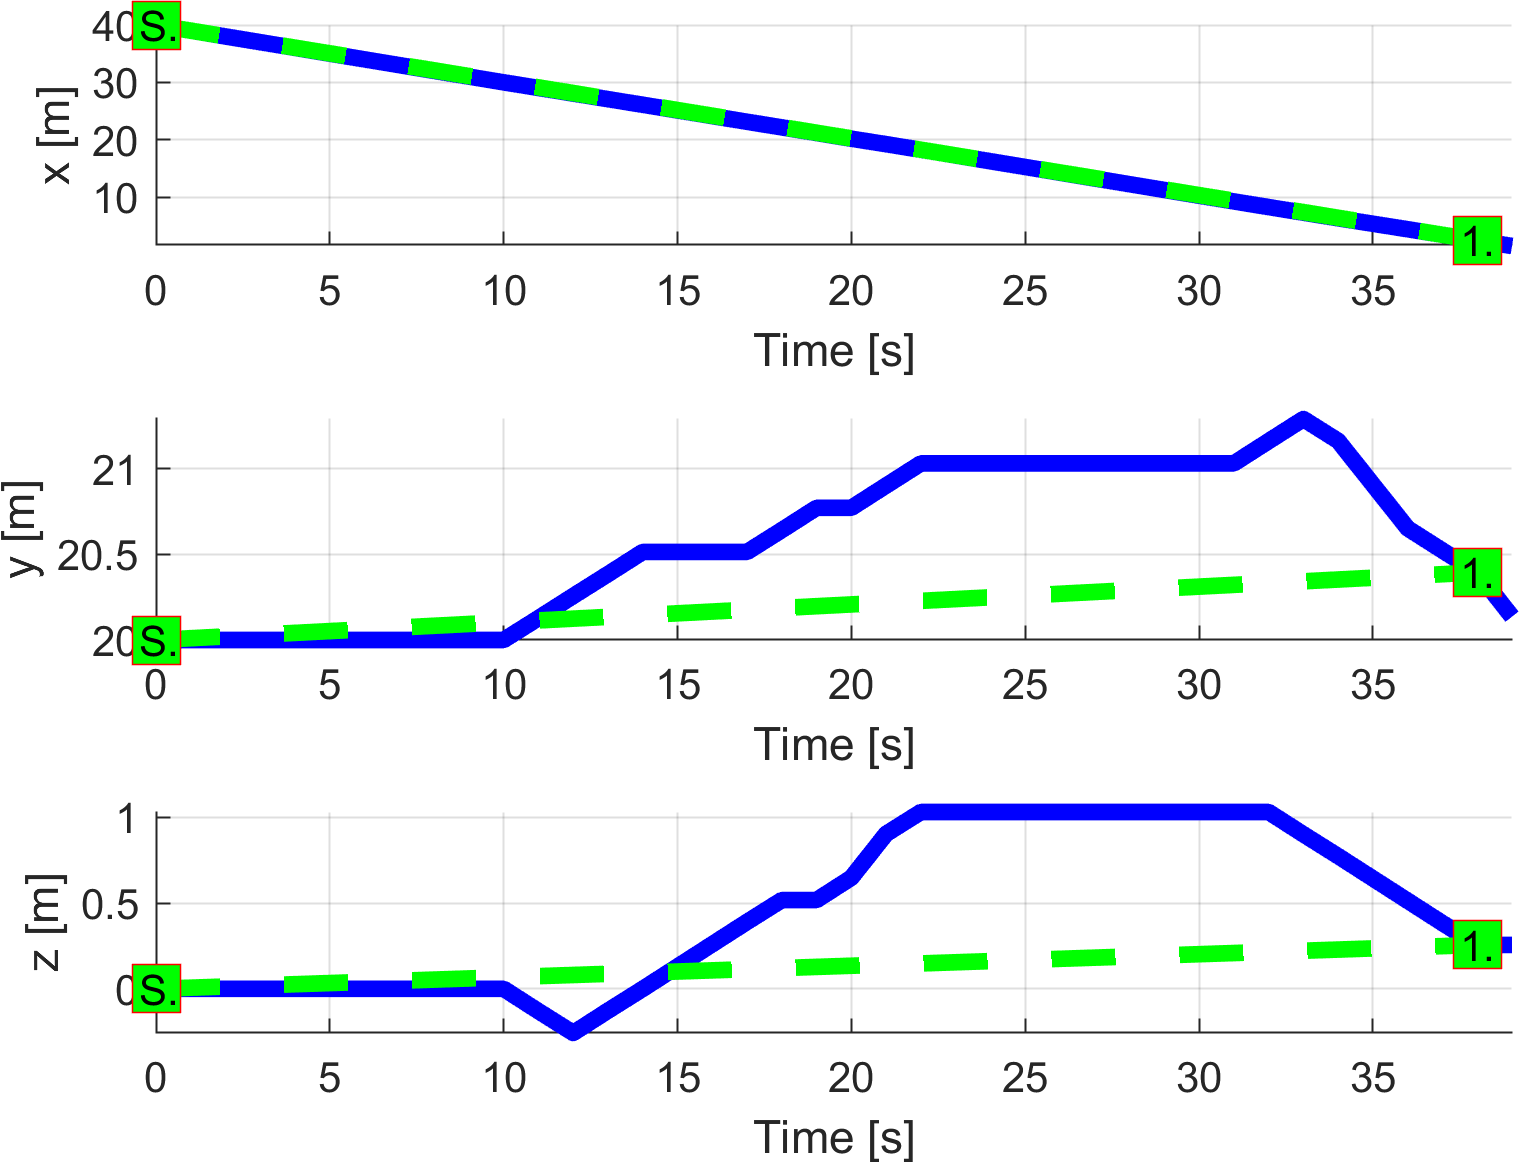
\includegraphics[width=0.9\linewidth]{\FIGDIR/NS038UtmEmergencyHeadOnUAV2PathFollowing} 
        \caption{UAS 2.}
        \label{fig:emergencyHeadOnUAS2PathTracking}
    \end{subfigure}
    \caption{\emph{Trajectory tracking} for \emph{Emergency head on} test case. }
    \label{fig:emergencyHeadOnTrajectoryTrackingPerformance}
\end{figure}


\paragraph{Path Following Deviations:} \emph{Deviations} (tab. \ref{tab:pathTrackingParametersForEmergencyHeadOn}) are in expected ranges considering the \emph{mission plans} (tab. \ref{tab:missionSetupEmergencyHeadOnScenario}) and \emph{separation safety margins} (tab. \ref{tab:aboidanceParametersForEmergencyHeadOnScenario}).


\begin{table}[H]
    \centering
    \begin{tabular}{c||c|c}
        \multirow{2}{*}{Param.} & UAS 1     & UAS 2\\\cline{2-3}
                        & $\mathscr{WP}_1$  & $\mathscr{WP}_1$\\\hline\hline
          $\max |x|$    & 0.05              & 0.06 \\\hline
          $\max |y|$    & 1.37              & 1.48 \\\hline
          $\max |z|$    & 1.03              & 1.05 \\\hline
          $\max dist.$  & 1.39              & 1.52 \\
    \end{tabular}
    \caption{Path tracking properties for \emph{Emergency head on} scenario.}
    \label{tab:pathTrackingParametersForEmergencyHeadOn}
\end{table}
    	\subsection{Emergency Mixed Head on with Converging}\label{s:testEmergencyMixed}

    \noindent\paragraph{Scenario:} \emph{Four UAS} are flying in an \emph{uncontrolled airspace} (altitude $\le$ 500 ft. Above the Ground Level) missions defined in (tab. \ref{tab:missionSetupEmergencyMixedScenario}). All UAS are in the \emph{Navigation mode} with active \emph{ADS-B In}, receiving \emph{position notifications} from each other. Cruising altitude is sufficient for \emph{horizontal separation} (50-100 ft. Above the Ground Level).
    
    
    \begin{table}[H]
        \centering
        \begin{tabular}{c||c|c||c}
            \multirow{2}{*}{UAS} &\multicolumn{2}{c||}{Position} & \multirow{2}{*}{$\mathscr{WP}_1$} \\\cline{2-3}
              & $[x,y,z]$           & $[\theta,\varpi,\psi]$           & \\\hline\hline
            1 & $[0,20,0]^T $       & $[0^\circ,0^\circ,0^\circ]^T$    & $[45,20,0]^T$\\\hline 
            2 & $[40,20,0]^T $       & $[0^\circ,0^\circ,180^\circ]^T$    & $[-5,20,0]^T$\\\hline 
            3 & $[20,0,0]^T $       & $[0^\circ,0^\circ,90^\circ]^T$    & $[20,45,0]^T$\\\hline 
            4 & $[20,40,0]^T $       & $[0^\circ,0^\circ,-90^\circ]^T$  & $[45,20,0]^T$\\ 
        \end{tabular}
        \caption{Mission setup for \emph{Emergency mixed} scenario.}
        \label{tab:missionSetupEmergencyMixedScenario}
    \end{table}
    
    \begin{note}
        \emph{Collision point} is expected at $\mathscr{C}=[20,20,0]^T$
    \end{note}
    
    \noindent \paragraph{Main Goal:} Show \emph{multiple non-cooperative intruders avoidance capability} in \emph{uncontrolled} airspace.
    
    \noindent \paragraph{Acceptance criteria:}
    \begin{enumerate}
        \item \emph{Proper avoidance mode invocation} - when an  \emph{intruder intersection model} impact the \emph{Avoidance Grid}, UAS system will switch to an \emph{Emergency avoidance mode}.
        
        \item\emph{Minimal safety margin distance} $\ge$ $0 m$.
        
        \item Each \emph{UAS} will reach own goal waypoint (tab. \ref{tab:missionSetupEmergencyMixedScenario}).
    \end{enumerate}
    
    
    \noindent\paragraph{Testing setup:} The \emph{standard test setup} for each UAS defined in (tab \ref{tab:testMovementOrientations}, \ref{tab:testUASBasicParameters}, \ref{tab:testNavigationGridBasic}, \ref{tab:testAvoidanceGridBasic}, \ref{tab:testUASColoring}) is used with following without parameter override.

    \emph{Intruder intersection} model has been chosen depending on UAS (tab. \ref{tab:aboidanceParametersForEmergencyMixedScenario}). Each UAS is equipped with \emph{ADS-B In/Out} sensor obtaining/distributing following information:
    \begin{enumerate}
        \item \emph{Position} - in operational section coordinate frame.
        \item \emph{Velocity} - vector representation in given coordinate frame.
        \item \emph{Class size} - class body radius based on UAS propulsion and size.
        \item \emph{Safety margin set} - set of safety margins for different collision cases.
    \end{enumerate}
    
    \emph{Avoidance parameters} for \emph{Emergency mixed scenario} are given in (tab. \ref{tab:aboidanceParametersForEmergencyMixedScenario}). Each UAS has different \emph{intruder model} and separation combination. Each UAS has same speed set to $1 m s^{-1}$. None of UAS has the \emph{Right of The Way}. 
    
    \emph{Safety margin} is considered as sum of both participants \emph{near miss margins}. In this case default safety margin is considered as $1.2$  $m$.
    
    \begin{table}[H]
        \centering
        \begin{tabular}{c||c|c|c||c|c||c}
            \multirow{2}{*}{UAS} & \multicolumn{3}{c||}{Parameters} & \multicolumn{2}{c||}{Margins} & \multirow{2}{*}{Separation}\\\cline{2-6}
                                 & velocity & intruder model & ROW        & body & safety                                        \\\hline\hline
            1                    & 1        & body + spread  & false            & 0.3         & 0.6           & horizontal       \\\hline
            2                    & 1        & body (timed)   & false            & 0.3         & 0.6           & vertical         \\\hline
            3                    & 1        & body (timed)   & false            & 0.3         & 0.6           & horizontal       \\\hline
            2                    & 1        & body + spread  & false            & 0.3         & 0.6           & vertical         \\
        \end{tabular}
        \caption{Avoidance parameters for  \emph{Emergency mixed} scenario.}
        \label{tab:aboidanceParametersForEmergencyMixedScenario}
    \end{table}
    
    \begin{note}
        Each \emph{UAS} use different intruder intersection models and primary \emph{separations} (defined in tab. \ref{tab:aboidanceParametersForEmergencyMixedScenario}).  UAS reactions are based on primary \emph{Separation} mode, intruders intersection models this is reflected on major axial deviations in (fig. \ref{fig:testCaseEmergencyMixedTrajectoryTracking}) and summarized in \emph{path tracking} deviation (tab. \ref{tab:pathTrackingParametersForEmergencyMixed}).
    \end{note}
    
    \noindent\paragraph{Simulation Run:} Notable moments from the simulation run (fig. \ref{fig:testCaseEmergencyMixed}) are following:
    
    \begin{enumerate}
        \item \emph{Situation detection} (fig. \ref{fig:emergencyMultipleSituationDetection}) - UAS 1 (blue) is detecting UAS 2 (cyan), UAS 3 (green), and UAS 4 (black) as possible intruders. There are multiple converging and head on approaches depending on mutual positions (UAS and \emph{angle of approach}). There exist at least one \emph{converging case} where each UAS has \emph{Right of the way}. Each UAS creates intruder intersection models depending on the intruder configuration (tab. \ref{tab:aboidanceParametersForEmergencyMixedScenario}). Each UAS enters into the \emph{Emergency avoidance mode} independently, when at least one trajectory is constrained in the \emph{avoidance grid}. 
        
        \item \emph{Before near miss} (fig. \ref{fig:emergencyMultipleBeforeNearMiss}) - all \emph{UAS} are in \emph{emergency avoidance mode}, using various \emph{separation modes} and \emph{intruder intersection models}. Each UAS is performing its own avoidance maneuver, constantly checking other intruders. If same separation and same intruder model was used, there will be virtual roundabout.
            
        \item \emph{After near miss} (fig. \ref{fig:emergencyMultipleAfterNearMiss}) - all \emph{UAS} avoided each other which is covered in \emph{safety margin performance} (fig. \ref{fig:testCaseMultipleAvoidancePerformance}) and (tab. \ref{tab:testCaseEmergencyMixedSafetyMarginDistances}).
        
        \item \emph{Situation resolution} (fig. \ref{fig:emergencyMultipleSituationReslution}) - all \emph{UAS}
        returns to \emph{Navigation mode} correcting \emph{altitude} first and continuing to assigned waypoints.
    \end{enumerate}
    
    \begin{figure}[H]
        \centering
        \begin{subfigure}{0.48\textwidth}
        	\centering
            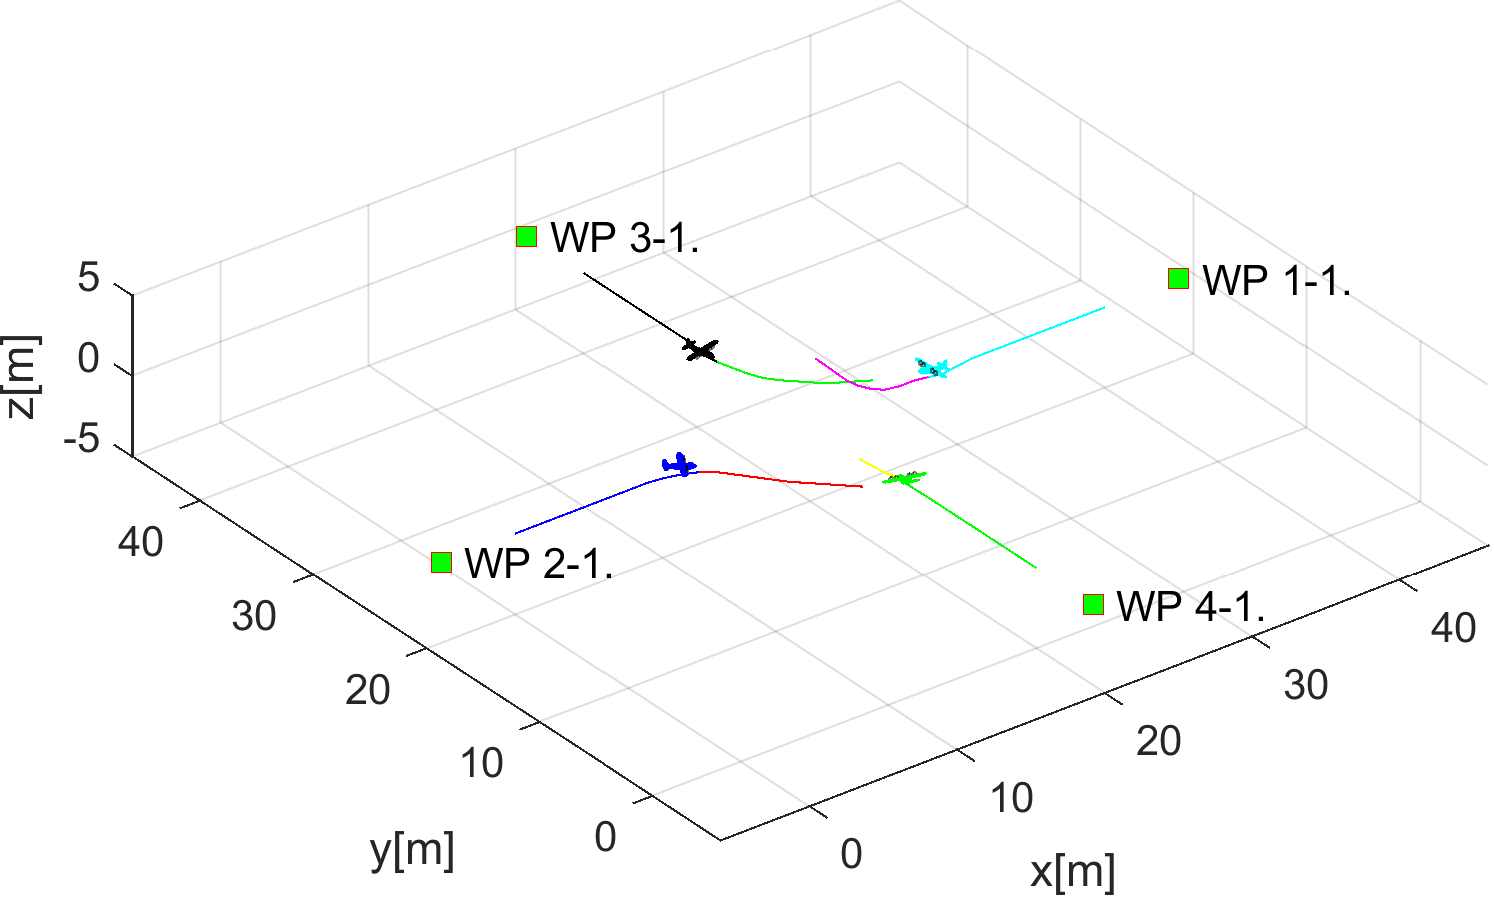
\includegraphics[width=0.9\linewidth]{\FIGDIR/NS039UtmEmergencyHeadOnMultiple00012}
            \caption{Situation detection.}
            \label{fig:emergencyMultipleSituationDetection}
        \end{subfigure}
        \begin{subfigure}{0.48\textwidth}
        	\centering
            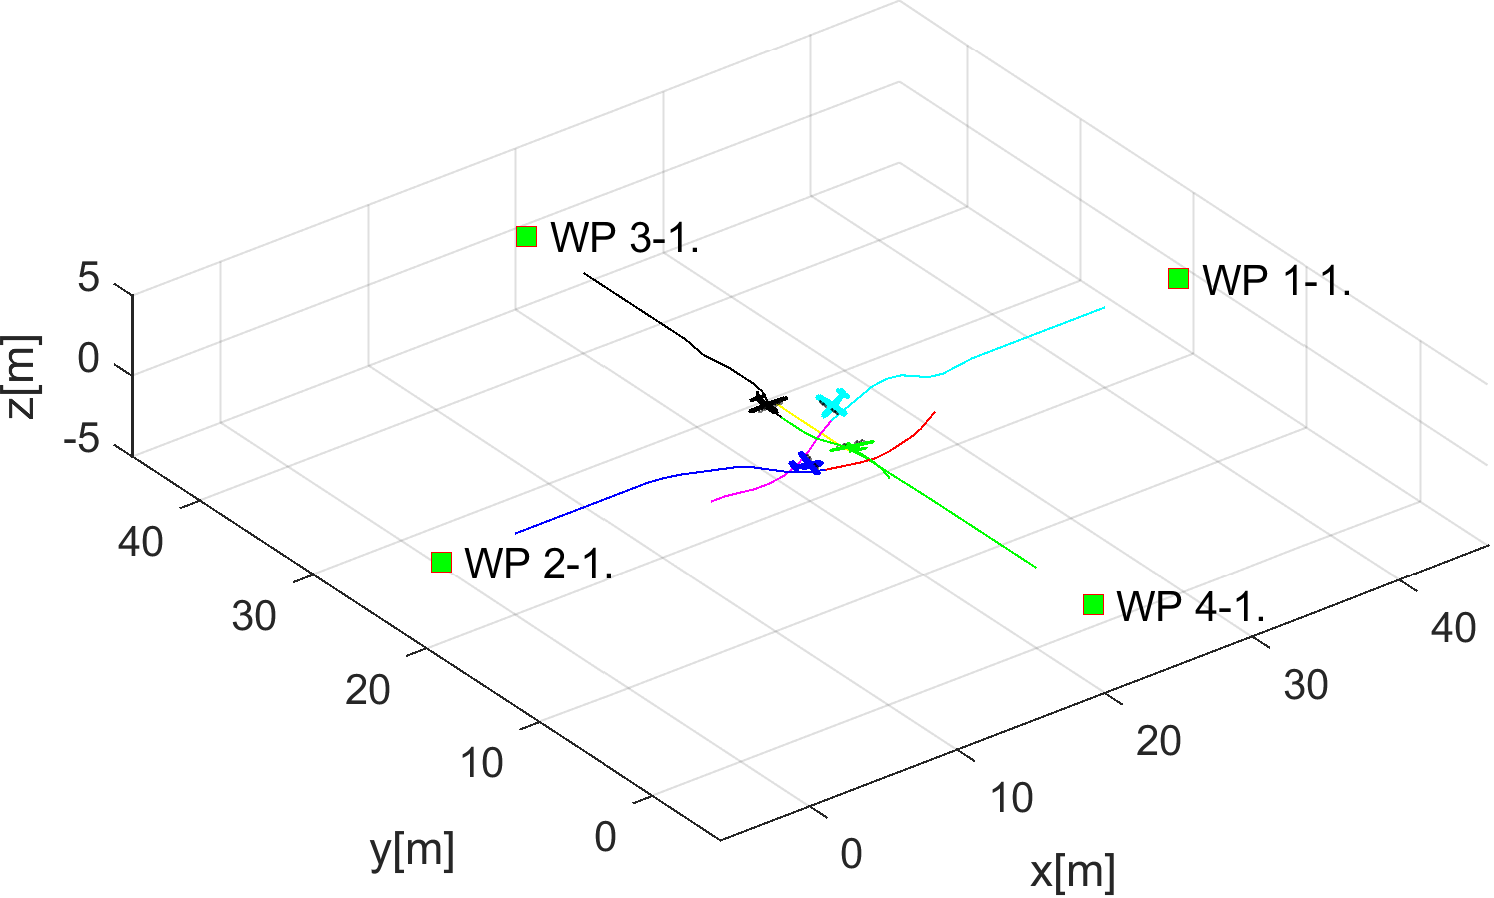
\includegraphics[width=0.9\linewidth]{\FIGDIR/NS040UtmEmergencyHeadOnMultiple00019} 
            \caption{Before near miss.}
            \label{fig:emergencyMultipleBeforeNearMiss}
        \end{subfigure}
        \\
        \begin{subfigure}{0.48\textwidth}
        	\centering
            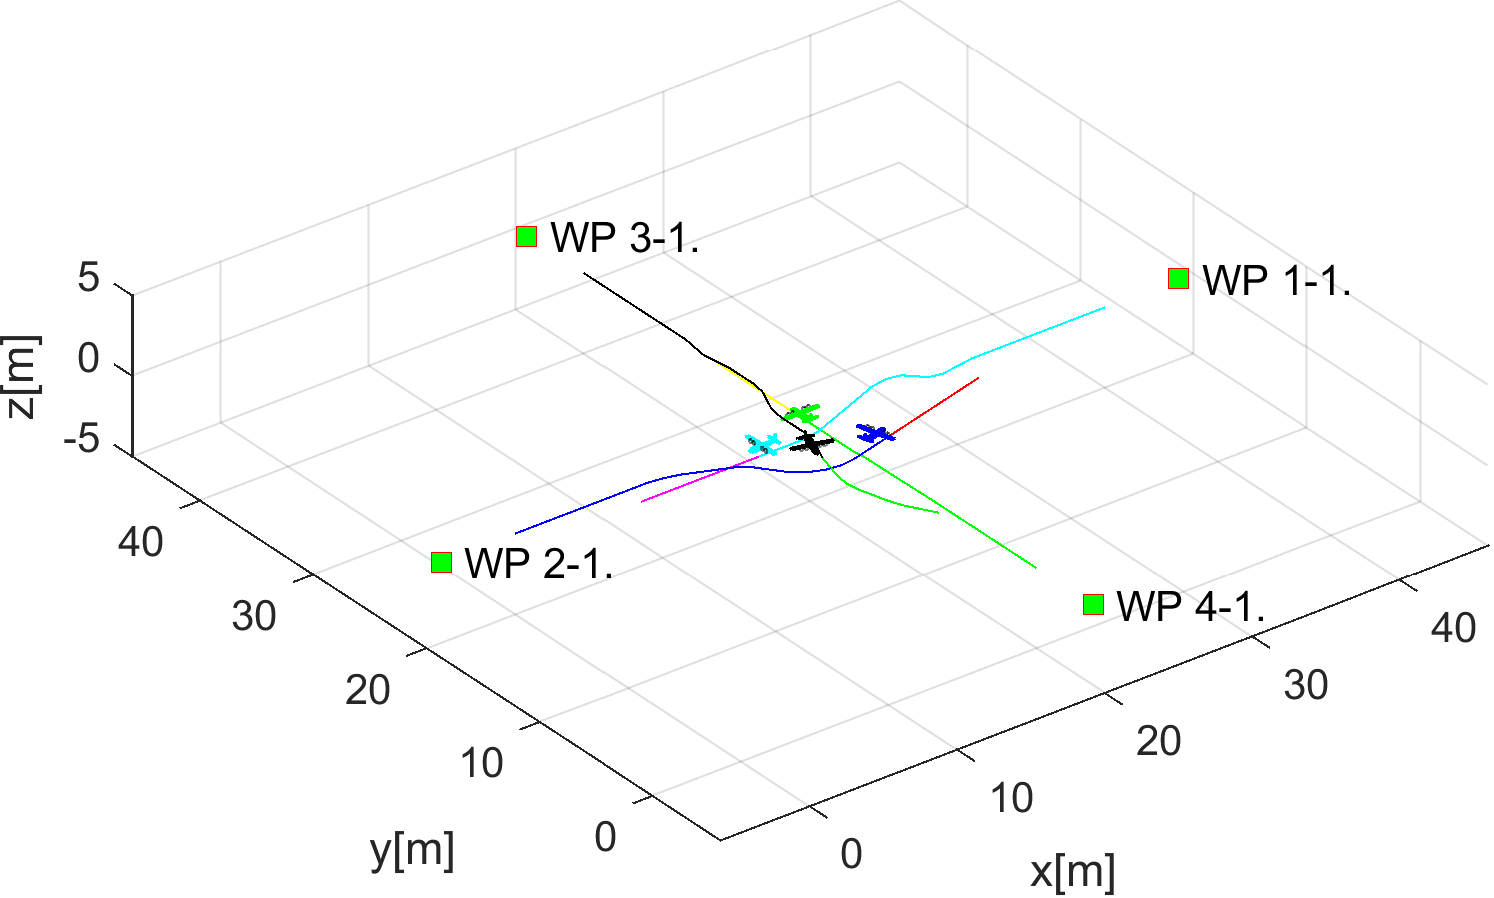
\includegraphics[width=0.9\linewidth]{\FIGDIR/NS041UtmEmergencyHeadOnMultiple00024} 
            \caption{After near miss.}
            \label{fig:emergencyMultipleAfterNearMiss}
        \end{subfigure}
        \begin{subfigure}{0.48\textwidth}
        	\centering
            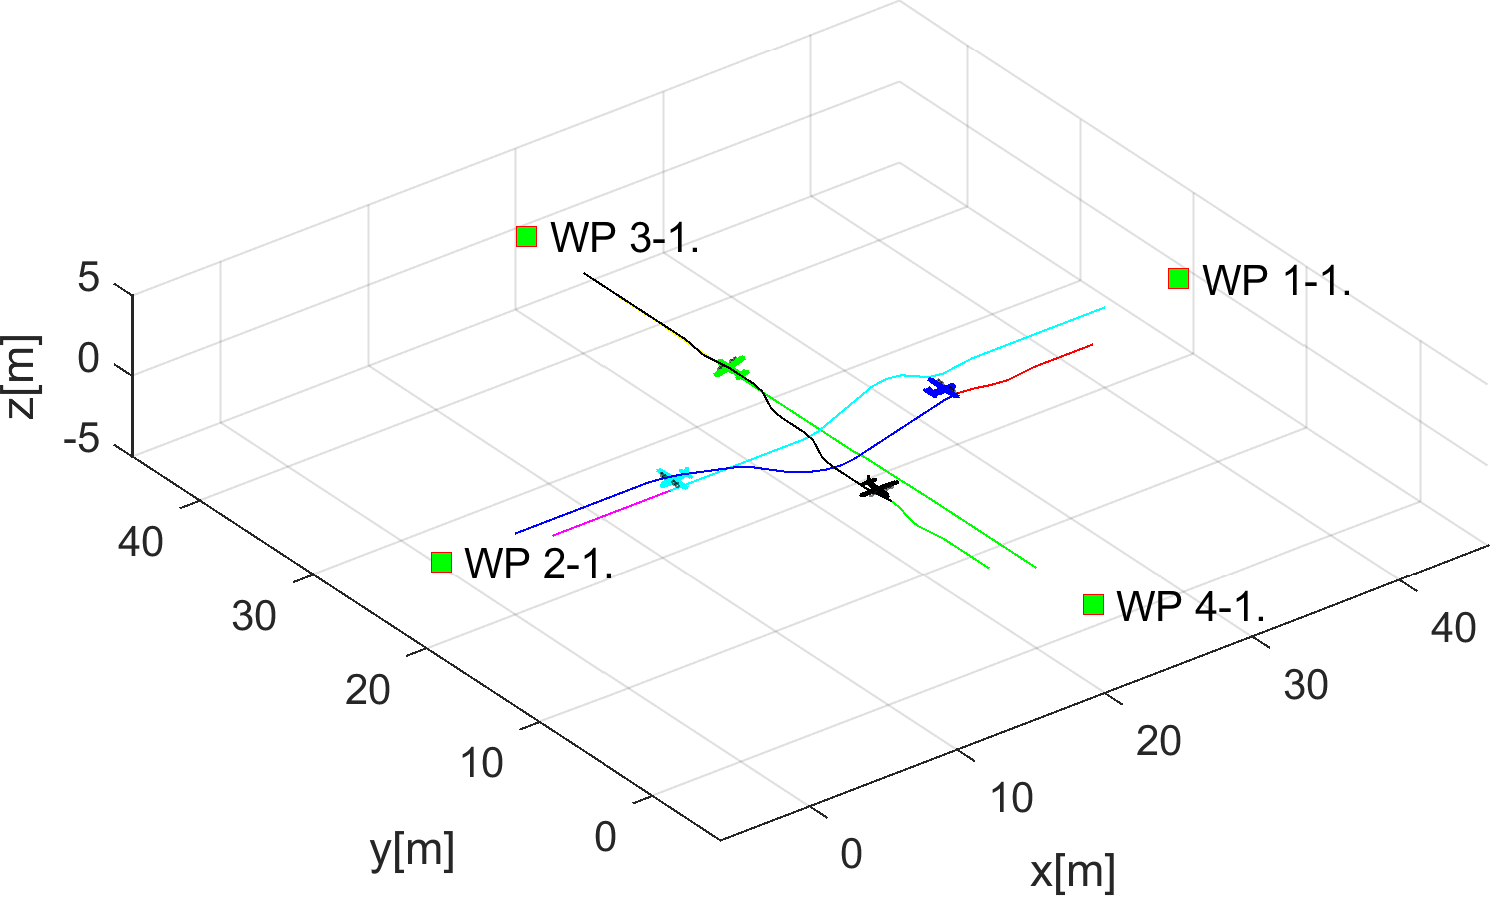
\includegraphics[width=0.9\linewidth]{\FIGDIR/NS042UtmEmergencyHeadOnMultiple00030} 
            \caption{Situation resolution.}
            \label{fig:emergencyMultipleSituationReslution}
        \end{subfigure}
        \caption{Test scenario for \emph{Emergency mixed} situation with \emph{self-separation mode}.}
        \label{fig:testCaseEmergencyMixed}
    \end{figure}
    
    \paragraph{Distance to Safety Margin Evolution:} There is need to compare mutual distance between each UAS. The graph (fig. \ref{fig:testCaseMultipleAvoidancePerformance}) shows six figures for each \emph{UAS systems} mutual distance (blue line) in this scenario. The \emph{Safety Margin} (red line) ($1.2$ $m$) was not breached for any pair (case). 
    
    The \emph{Proper avoidance invocation} is shown when UAS systems are getting closer to each other and then they start separation phase (Emergency avoidance mode).
            
    \begin{figure}[H]
        \centering
        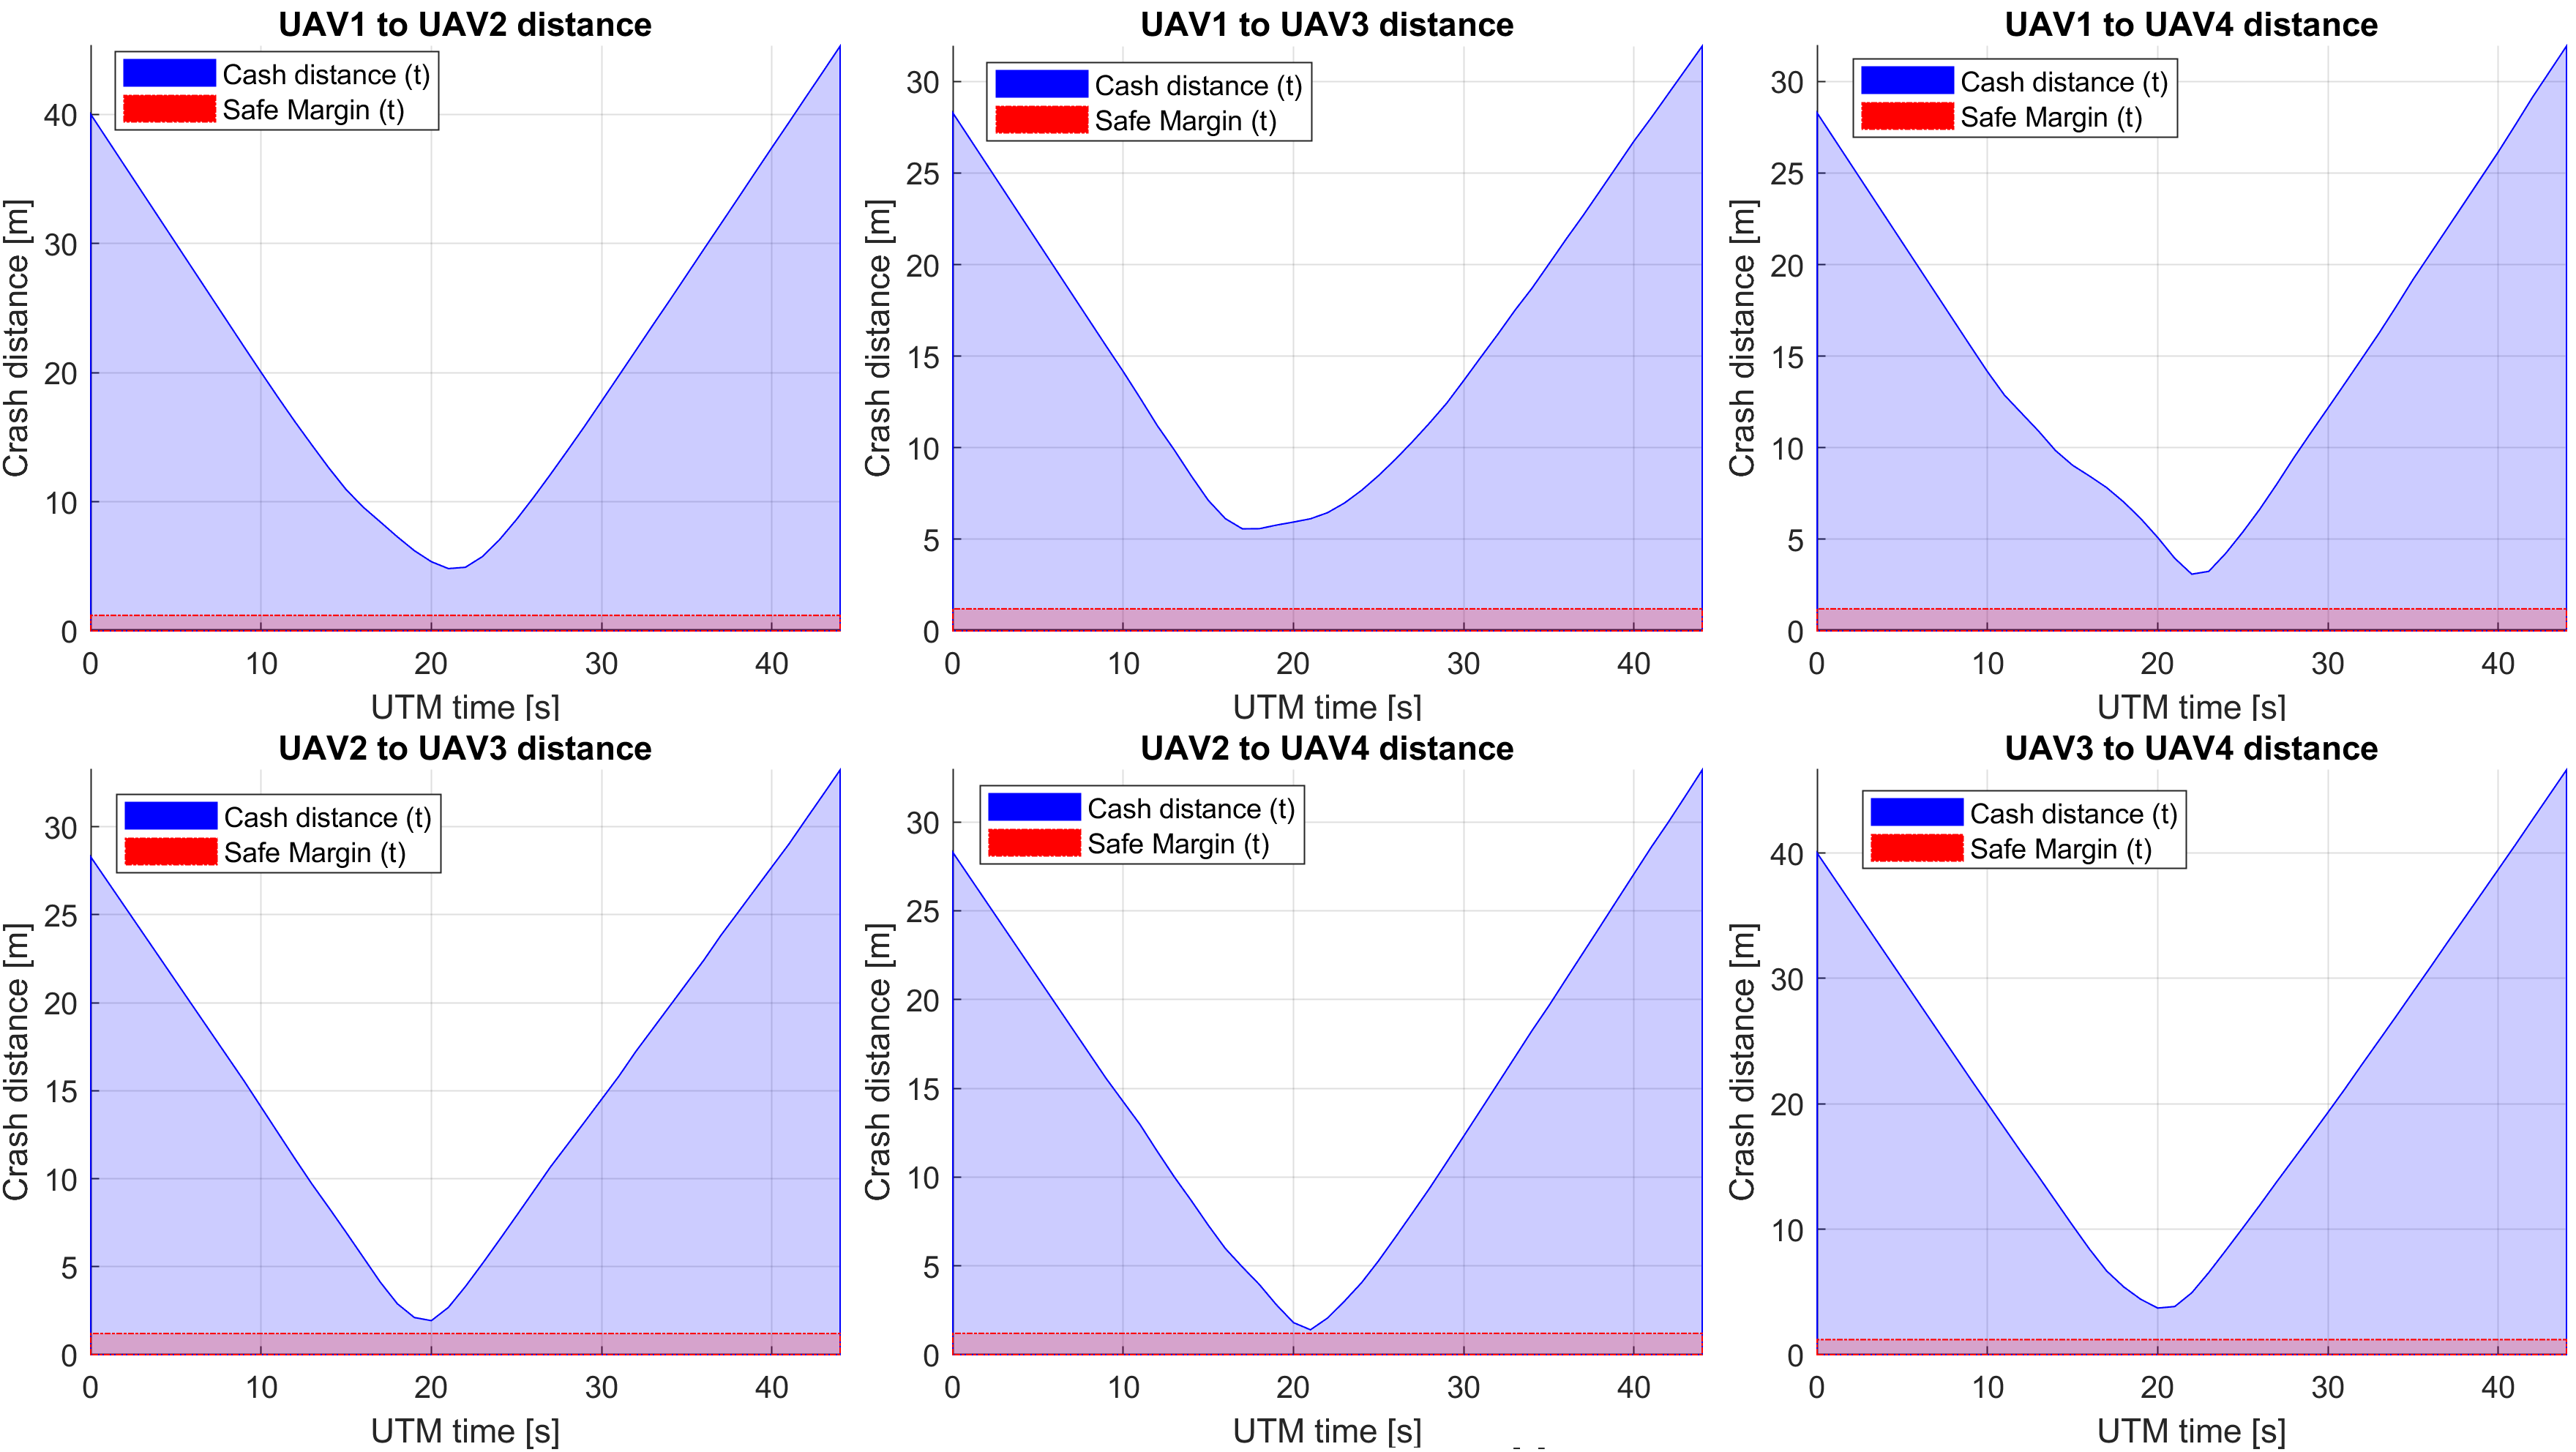
\includegraphics[width=0.9\linewidth]{\FIGDIR/NS043UtmEmergencyHeadOnMultiplePerformance} 
        \caption{Distance to safety margin evolution for \emph{emergency mixed scenario}.}
        \label{fig:testCaseMultipleAvoidancePerformance}
    \end{figure}
    
    \paragraph{Distance to Safety Margin Peaks:} Minimal and Maximal mutual distance to safety margin is summarized in (tab. \ref{tab:testCaseEmergencyMixedSafetyMarginDistances}). There is no detected breach for any combination. 
    
    The \emph{closest to collision} is UAS pair $2-4$ with mutual safety margin only $0.2019$ $m$. On the other side is UAS pair $1-3$ with mutual safety margin $4.3721$ $m$. 
    
    The \emph{minimal distance to safety margin}  $\ge$ 0 which means that the \emph{safety condition} is fulfilled. 
    
    \begin{table}[H]
        \centering
        \begin{tabular}{c||c|c|c}
            \multirow{2}{*}{UAS:} & \multicolumn{3}{c}{Distance to Safety Margin} \\ \cline{2-4} 
                      & min          & max         & breach         \\ \hline\hline
                1-2   & 3.6231       & 44.0831     & false          \\ \hline
                1-3   & 4.3721       & 30.7300     & false          \\ \hline
                1-4   & 1.8959       & 30.7331     & false          \\ \hline
                2-3   & 0.7331       & 32.0266     & false          \\ \hline
                2-4   & 0.2019       & 31.7282     & false          \\ \hline
                3-4   & 2.5171       & 45.4257     & false          \\ 
        \end{tabular}
        \caption{Distance to safety margin peaks for \emph{emergency mixed scenario}.}
        \label{tab:testCaseEmergencyMixedSafetyMarginDistances}
    \end{table}
    
    \noindent\paragraph{Path Tracking Performance:} All waypoints (Green numbered squares) for all UAS have been reached (fig. \ref{fig:testCaseEmergencyMixedTrajectoryTracking}). \emph{Reference trajectories} (green dashed line) have been tracked by \emph{UAS real path} (blue solid line) almost all time. 
    
    Following observations can be made from \emph{path tracking} (fig. \ref{fig:testCaseEmergencyMixedTrajectoryTracking}) and \emph{preferred separations} (tab. \ref{tab:aboidanceParametersForEmergencyMixedScenario}):
    
    \begin{enumerate}
        \item UAS 1 (fig. \ref{fig:emergencyMixedPathTrackingUAS1}) is using \emph{horizontal separation} (y axis right) having \emph{preferred horizontal separation}.
        
        \item UAS 2 (fig. \ref{fig:emergencyMixedPathTrackingUAS2}) is using vertical separation (z axis up-down), having preferred vertical separation.
        
        \item UAS 3 (fig. \ref{fig:emergencyMixedPathTrackingUAS3}) is using horizontal/vertical separation (x right, z down), having preferred horizontal separation.  This UAS has used other than preferred separation type.
        
        \item UAS 4 (fig. \ref{fig:emergencyMixedPathTrackingUAS4}) is using horizontal separation (x-axis right/left), having preferred vertical separation. This UAS has used opposite separation type, than preferred.
    \end{enumerate}
    
    
    \begin{figure}[H]
        \centering
        \begin{subfigure}{0.48\textwidth}
        	\centering
            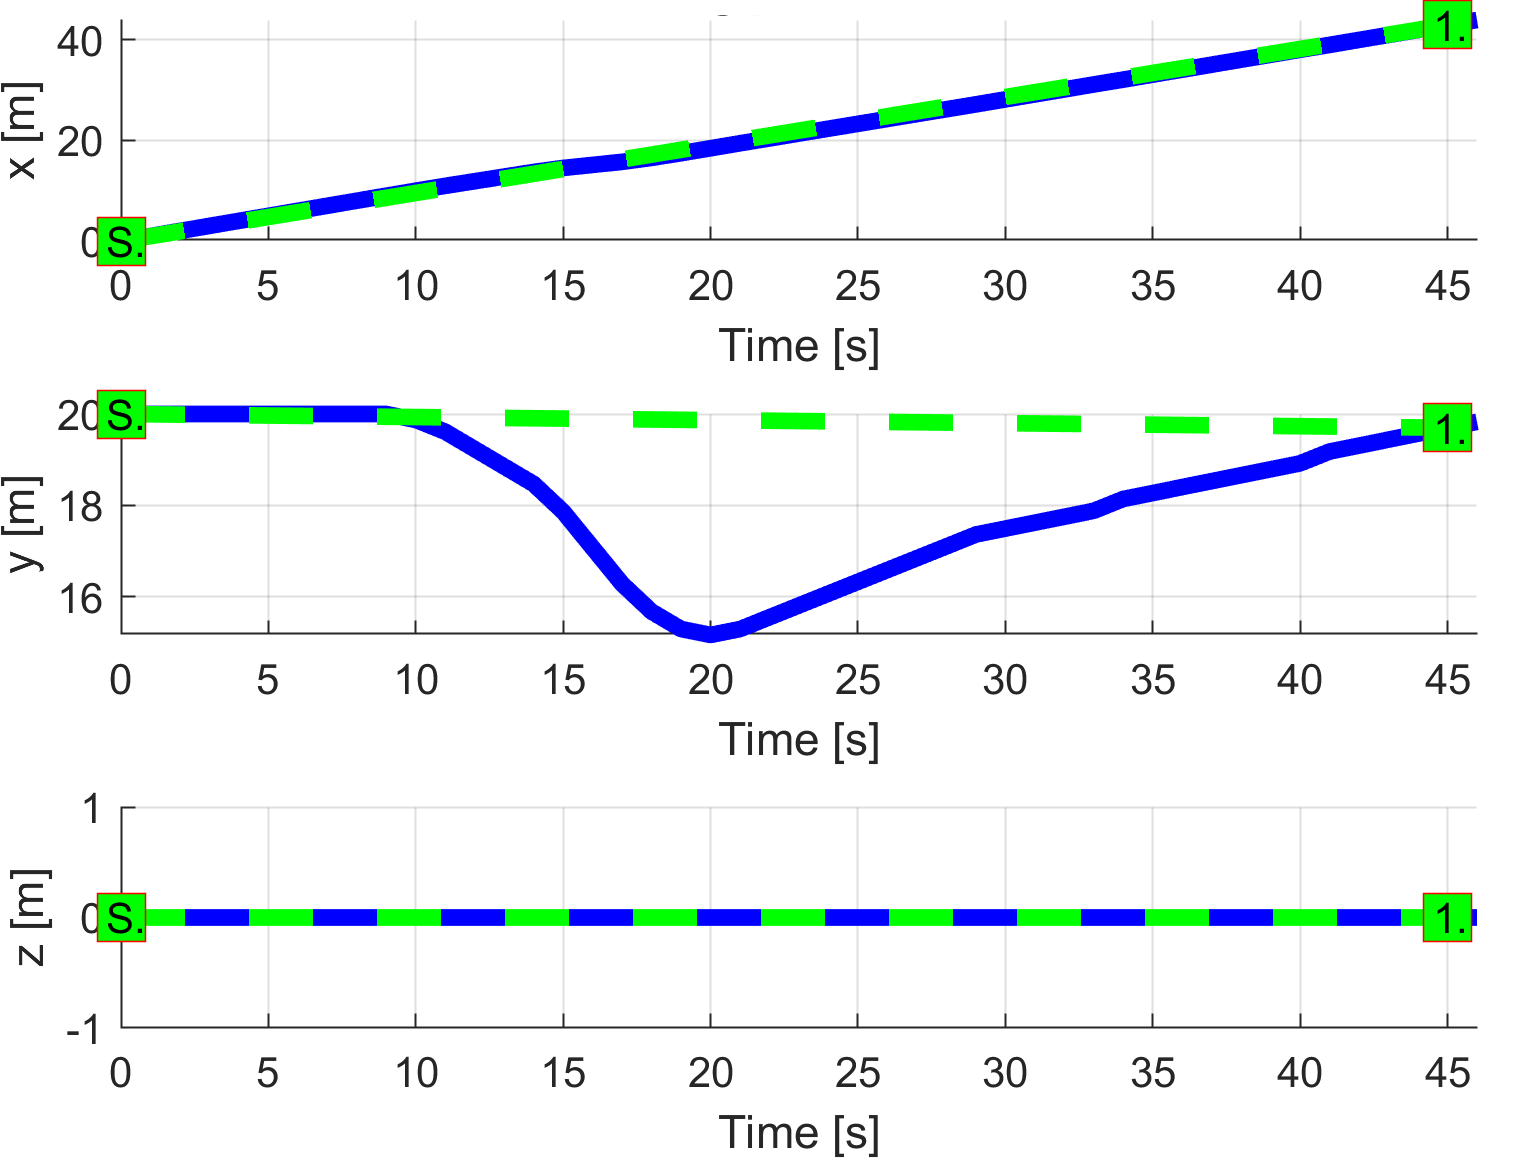
\includegraphics[width=0.9\linewidth]{\FIGDIR/NS044UtmEmergencyHeadOnMultipleUAV1PathFollowing}
            \caption{UAS 1.}
            \label{fig:emergencyMixedPathTrackingUAS1}
        \end{subfigure}
        \begin{subfigure}{0.48\textwidth}
        	\centering
            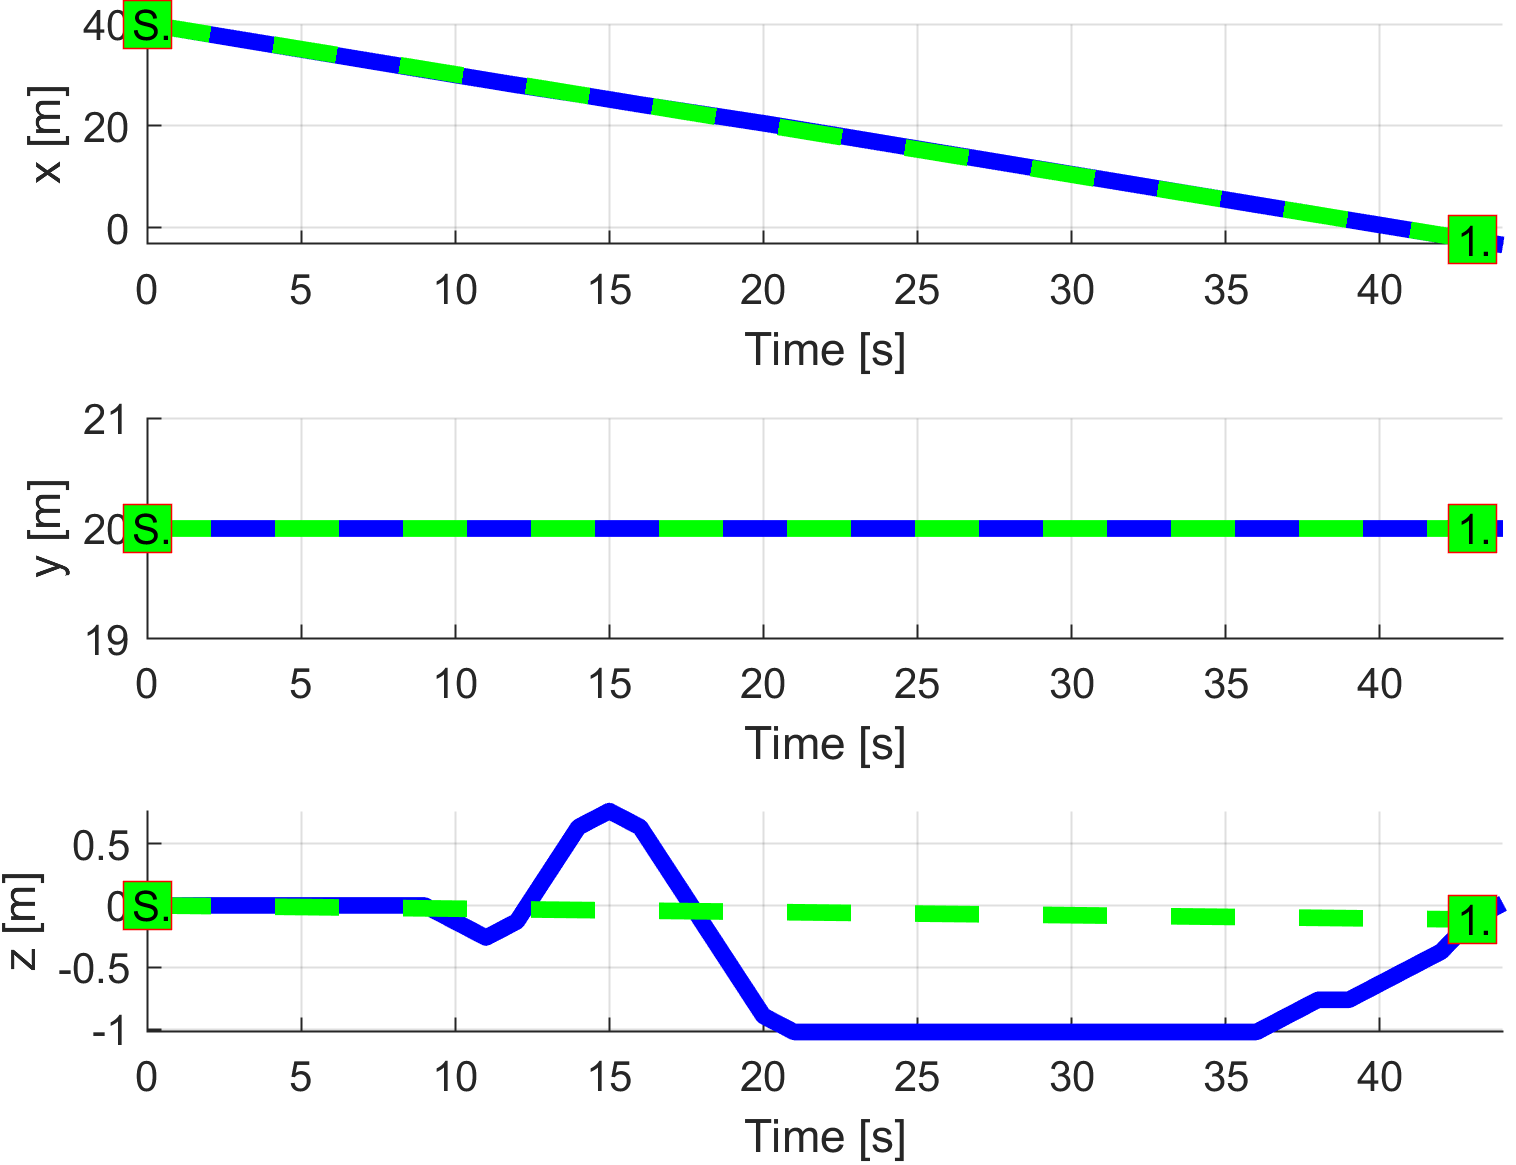
\includegraphics[width=0.9\linewidth]{\FIGDIR/NS045UtmEmergencyHeadOnMultipleUAV2PathFollowing} 
            \caption{UAS 2.}
            \label{fig:emergencyMixedPathTrackingUAS2}
        \end{subfigure}
        \\
        \begin{subfigure}{0.48\textwidth}
        	\centering
            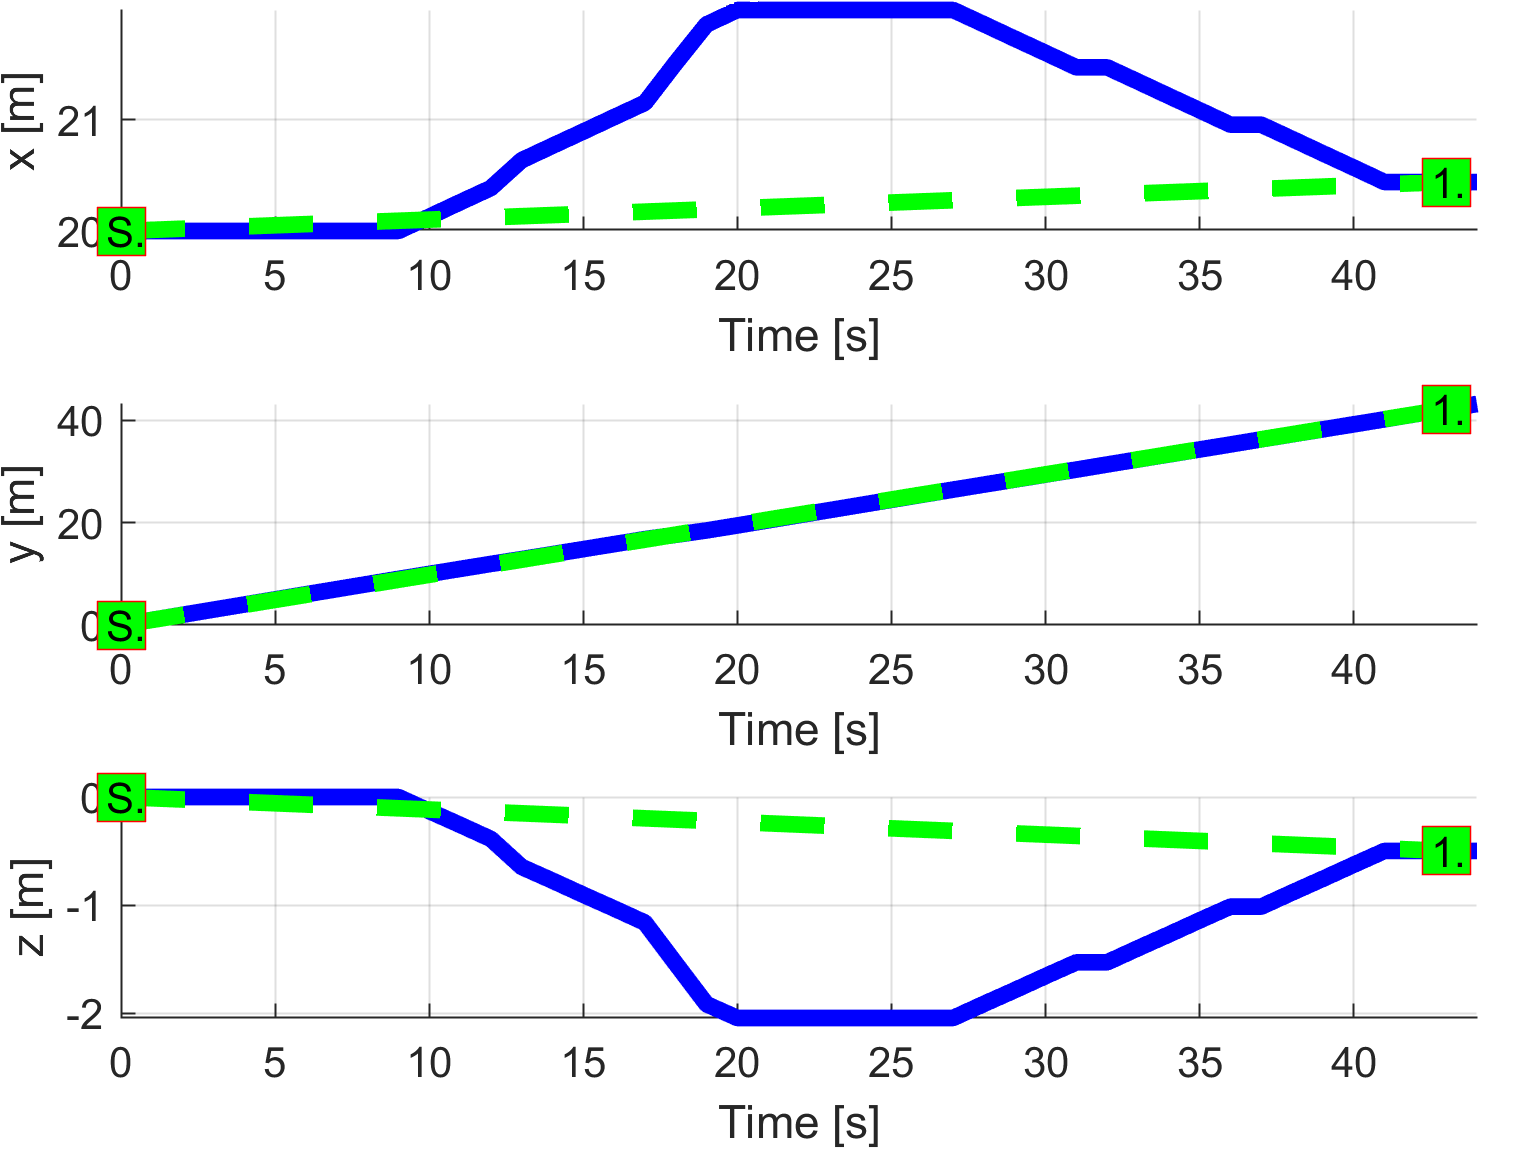
\includegraphics[width=0.9\linewidth]{\FIGDIR/NS046UtmEmergencyHeadOnMultipleUAV3PathFollowing} 
            \caption{UAS 3.}
            \label{fig:emergencyMixedPathTrackingUAS4}
        \end{subfigure}
        \begin{subfigure}{0.48\textwidth}
        	\centering
            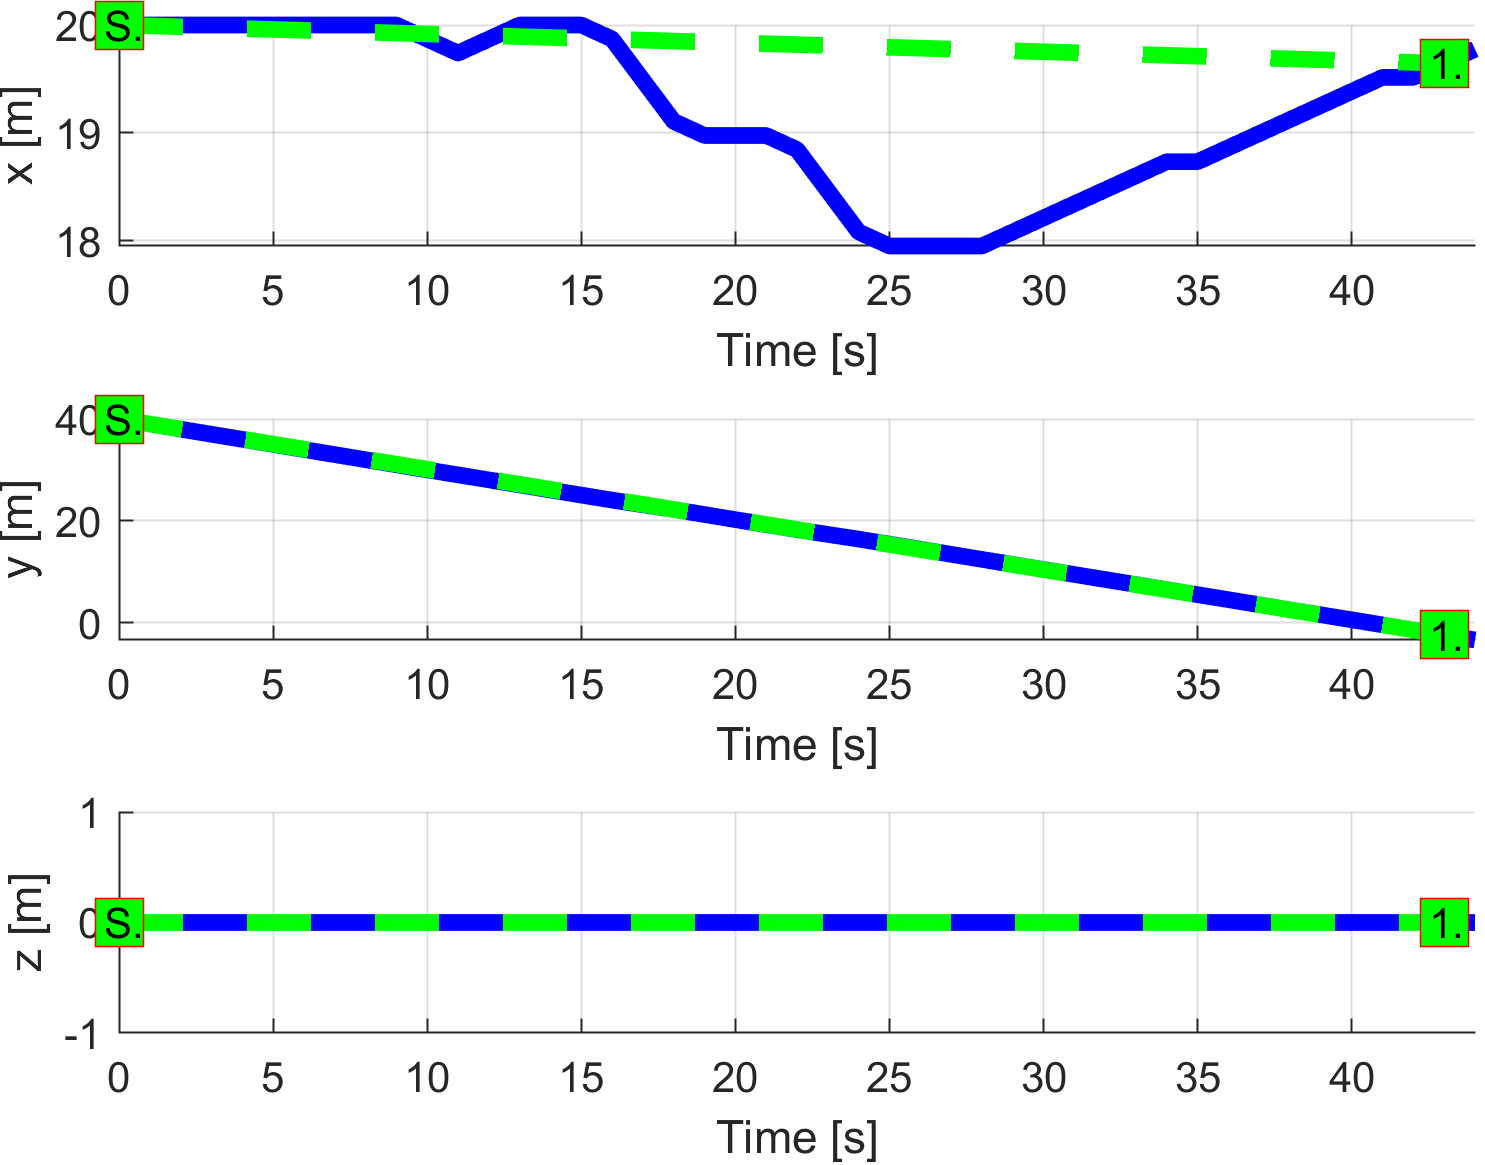
\includegraphics[width=0.9\linewidth]{\FIGDIR/NS047UtmEmergencyHeadOnMultipleUAV4PathFollowing} 
            \caption{UAS 4.}
            \label{fig:emergencyMixedPathTrackingUAS3}
        \end{subfigure}
        \caption{Trajectory tracking for \emph{Emergency mixed} situation test case.}
        \label{fig:testCaseEmergencyMixedTrajectoryTracking}
    \end{figure}
    
    \noindent\paragraph{Path Tracking Deviations:} \emph{Deviations} (tab. \ref{tab:pathTrackingParametersForEmergencyMixed}) are in expected ranges considering the \emph{mission plans} (tab. \ref{tab:missionSetupEmergencyMixedScenario}) and \emph{separation safety margins} (tab. \ref{tab:aboidanceParametersForEmergencyMixedScenario}).
    
    \begin{table}[H]
        \centering
        \begin{tabular}{c||c|c|c|c}
            \multirow{2}{*}{Param.} & UAS 1     & UAS 2             & UAS 3             & UAS 4 \\\cline{2-5}
                            & $\mathscr{WP}_1$  & $\mathscr{WP}_1$  & $\mathscr{WP}_1$  & $\mathscr{WP}_1$ \\\hline\hline
              $\max |x|$    & 0                 & 0                 & 1.98              & 2.05\\\hline
              $\max |y|$    & 4.84              & 0                 & 0                 & 0\\\hline
              $\max |z|$    & 0                 & 1.23              & 2.43              & 0\\\hline
              $\max dist.$  & 4.84              & 1.23              & 3.45              & 2.05\\
        \end{tabular}
        \caption{Path tracking properties for \emph{Emergency mixed} scenario.}
        \label{tab:pathTrackingParametersForEmergencyMixed}
    \end{table}    



    
    \cleardoublepage
\section{\secState{D}Cooperative Test Cases}\label{s:cooperativeTestCases}
    
    \noindent The \emph{main goal} of this section is to show the operational capabilities of \emph{approach} under \emph{UTM supervision}. The minimal UTM functionality set (sec. \ref{sec:UASTrafficManagement}) has been implemented, including \emph{position notifications mechanism, collision case calculation, resolution enforcement} components. 
    
    Test cases covers \emph{well clear breach prevention}, \emph{situation based avoidance}, and \emph{rules of the air enforcement}. 
    
    Coverage of \emph{near miss situations}, \emph{clash incidents} is given implicitly by \emph{safety} and \emph{body} margins (tab. \ref{tab:controlledAirspaceViolations}).
    
    \begin{enumerate}
        \item \emph{Rule based converging} (sec. \ref{s:testRuleConverging}) covers \emph{well clear breach} and \emph{converging rule of the air}, showing determinism and \emph{UTM resolution execution}.
        
        \item \emph{Rule based head on} (sec. \ref{s:testRuleHeadOn}) covers \emph{well clear breach} and \emph{head on rule of the air}, showing determinism and \emph{UTM resolution execution}.
        
        \item \emph{Rule based mixed head on with converging} (sec. \ref{s:testRuleMixed}) covers \emph{well clear breach} and \emph{head on and converging rules of the air}. The main focus is on \emph{virtual roundabout} concept, when multiple collision cases are clustered into one avoidance maneuver. 
        
        \item \emph{Rule based overtake} (sec. \ref{s:testRuleOvertake}) covers \emph{well clear breach} during \emph{overtake} by faster UAS.
    \end{enumerate}


    	\subsection{Rule based Converging}\label{s:testRuleConverging}

\paragraph{Scenario:} Two \emph{UAS} are approaching an \emph{airway intersection} at \emph{same time} in \emph{controlled airspace} (over 500 feet Above the Ground Level). The mutual position of \emph{UAS} can be classified as \emph{Side approach}. Following \emph{collision hazards} are present:

\begin{enumerate}
    \item \emph{Active Converging Collision Hazard} -  There is an \emph{UAS} approaching from the \emph{right side}, which give him \emph{Right of the Way} and invokes need to actively avoid \emph{Intruder}.

	\item \emph{Passive Converging Collision Hazard} - There is an \emph{UAS} approaching from the \emph{left side}, which gave us \emph{Right of the Way} and imposes an obligation of \emph{active avoidance} on other \emph{UAS}.
	
\end{enumerate}


\noindent\emph{Collision Hazards} must be addressed by \emph{UTM} service in the following manner:


\begin{enumerate}
	\item \emph{Each UAS} in particular \emph{Controlled Space} periodically sends synchronized \emph{Position Notification} messages (tab. \ref{tab:positionNotification}). 
	
	\item \emph{UTM} service receives \emph{Position Notifications} and manages \emph{Collision Case} (tab. \ref{tab:collisionCase}) in \emph{Controlled Space}. 
	
	\item \emph{UTM} detects \emph{Converging Collision Case} with \emph{Collision Point} in  vicinity.
	
	\item \emph{UTM} service Sends \emph{Mandate} to UAS without \emph{Right of the Way} and implements \emph{Normative Directive} on all \emph{UAS} in area.
\end{enumerate}


\noindent\emph{Mission parameters} for both UAS systems are defined in (tab. \ref{tab:missionSetupRuleBasedConvergingScenario}).

\begin{table}[H]
    \centering
    \begin{tabular}{c||c|c||c}
        \multirow{2}{*}{UAS} &\multicolumn{2}{c||}{Position} & \multirow{2}{*}{$\mathscr{WP}_1$} \\\cline{2-3}
          & $[x,y,z]$           & $[\theta,\varpi,\psi]$           & \\\hline\hline
        1 & $[0,20,0]^T $       & $[0^\circ,0^\circ,0^\circ]^T$    & $[40,20,0]^T$\\\hline 
        2 & $[20,0,0]^T $       & $[0^\circ,0^\circ,90^\circ]^T$    & $[20,40,0]^T$\\
    \end{tabular}
    \caption{Mission setup for \emph{Rule based converging} scenario.}
    \label{tab:missionSetupRuleBasedConvergingScenario}
\end{table}


\paragraph{Assumptions:} Following assumptions are valid for this test:

\begin{enumerate}
	\item \emph{Controlled Airspace Airworthiness} - UAS system is equipped with necessary controlled airspace equipment like ADS-B In/Out, Radar, Transponder, etc. Moreover airworthy \emph{UAS} has capability to precisely follow \emph{UTM directives} (max. 5 $\%$ deviation).
	
	\item \emph{C2 (Command \& control) Link Established} - necessary for (UAS $\leftrightarrow$ UAS) and (UAS $\leftrightarrow$ UTM) communication. If \emph{C2} link is lost the \emph{UAS} will enter into \emph{Emergency avoidance mode}.
	
	\item \emph{Decision frame synchronization with UTM} - necessary in discrete C2 environment otherwise \emph{safety margins} needs to be \emph{bloated}.
	
	\item \emph{Both UAS have identical cruising speed} - simplification impacting \emph{UTM} service implementation. \emph{Obstacle Avoidance Framework} can comprehend various intruders speed, with proper \emph{UAS} directives.
\end{enumerate}

\paragraph{Main Goal:} Show possibility of \emph{Converging situation resolution} with \emph{forced safety margin} by \emph{UAS Traffic Management} system.  The \emph{Obstacle Avoidance Framework based on Reach Sets} is used as \emph{Navigation Module}.

\paragraph{Acceptance  Criteria:} Following criteria must be met:

\begin{enumerate}
	\item \emph{Well Clear Condition valid for both UAS} - Both \emph{UAS} must have \emph{minimal required distance} from \emph{other UAS} for all \emph{Converging Maneuver} enforcement time.
	
	\item \emph{Fulfillment of UTM Directives} - Both UAS must stay in \emph{Navigation mode} for all \emph{Converging Maneuver} enforcement time. \emph{UAS without Right Of the Way} must stay away for necessary time, before returning to \emph{Original Navigation waypoint $\mathscr{WP}_1$} following.
\end{enumerate}


\paragraph{Testing Setup:} The \emph{standard test setup} for each UAS defined in (tab. \ref{tab:testMovementOrientations}, \ref{tab:testUASBasicParameters}, \ref{tab:testNavigationGridBasic}, \ref{tab:testAvoidanceGridBasic}, \ref{tab:testUASColoring}) is used with following parameter override:
\begin{enumerate}
	\item \emph{Navigation grid - type} - \emph{ACAS-like} with enabled \emph{Horizontal maneuvers}
\end{enumerate}

This \emph{configuration} is based on assumption that every UAS is in \emph{controlled airspace} in \emph{FL450} (flight level 45000 feet Above Sea Level), without permission for \emph{climb or descent maneuver}. \emph{Rule engine} is initialized in standard \emph{Rules of the air} configuration (fig. \ref{fig:RuleEngineInstanceLevels}).

There is \emph{UTM} service for given \emph{airspace cluster} calculating \emph{collision cases} (tab. \ref{tab:collisionCase}) based on incoming \emph{UAS position notifications} (tab. \ref{tab:positionNotification}).

\paragraph{Simulation Run:} Notable moments from \emph{simulation run} (fig. \ref{fig:testCaseRuleBasedConverging}) are following:

\begin{enumerate}
    \item \emph{Collision Case creation} (fig. \ref{fig:ruleBasedConvergingCollisionCaseCreation}) following events happens in this step:
    \begin{enumerate}[a.]
        \item Two \emph{UAS} are approaching  \emph{airway intersection}: UAS 1 (blue) from left and UAS 2 (cyan) from bottom.
        
        \item They are going to \emph{collide} at point $\mathscr{C}=[20,20,0]^T$ of \emph{Flight Level} (elevation is 45, 000 feet Above Mean Seal Level).
        
        \item UTM service notices future \emph{Collision Situation} and creates \emph{Collision Case}.
        
        \item \emph{Converging Directive} for 8 m from \emph{Collision point} is issued for UAS 1 (blue), because UAS 2 (cyan) has \emph{Right Of the Way}.
        
        \item \emph{Keep Velocity/Heading Directive} is issued for UAS 2 (cyan) to ensure avoidance maneuver success.
        
        \item UAS 1 (blue) corrects its heading according to \emph{UTM} directive.
        
        \item UAS 2 (cyan) stays on claimed course and if its necessary adjust its speed.
        
    \end{enumerate}
    
    \item \emph{Well clear before} (fig. \ref{fig:ruleBasedConvergingWellClearBefore}) UAS 1 (blue) checks the \emph{Collision Point} distance and keeps safe distance given by safety margin. UAS 2 (cyan) checks if there is no intruder in \emph{Avoidance Grid} and if not, stays in \emph{Navigation Mode}.
    
    \item \emph{Well clear after} (fig. \ref{fig:ruleBasedConvergingWellClearAfter}) UAS 2 (cyan) is \emph{after Collision Point}, it can start negotiations of new speed and heading with UTM. UAS 1 (blue) is still enforced to follow \emph{Converging Maneuver} directive, until the outer boundary of \emph{Collision Zone} is reached.
    
    \item \emph{Waypoints reach} (fig. \ref{fig:ruleBasedConvergingWaypointsReach})  UAS 1 (blue) leaves outer boundary of \emph{Collision zone}. Leaving \emph{Converging Maneuver Directive}. UTM closes \emph{Collision Case}.
\end{enumerate}


\begin{figure}[H]
    \centering
    \begin{subfigure}{0.48\textwidth}
    	\centering
        \includegraphics[width=0.9\linewidth]{\FIGDIR/NS048UtmCooperativeConverging00003}
        \caption{Collision case creation.}
        \label{fig:ruleBasedConvergingCollisionCaseCreation}
    \end{subfigure}
    \begin{subfigure}{0.48\textwidth}
    	\centering
        \includegraphics[width=0.9\linewidth]{\FIGDIR/NS049UtmCooperativeConverging00016} 
        \caption{Well clear before.}
        \label{fig:ruleBasedConvergingWellClearBefore}
    \end{subfigure}
    \\
    \begin{subfigure}{0.48\textwidth}
    	\centering
        \includegraphics[width=0.9\linewidth]{\FIGDIR/NS050UtmCooperativeConverging00024} 
        \caption{Well clear after.}
        \label{fig:ruleBasedConvergingWellClearAfter}
    \end{subfigure}
    \begin{subfigure}{0.48\textwidth}
    	\centering
        \includegraphics[width=0.9\linewidth]{\FIGDIR/NS051UtmCooperativeConverging00037} 
        \caption{Waypoints reach.}
        \label{fig:ruleBasedConvergingWaypointsReach}
    \end{subfigure}
    \caption{Test scenario for \emph{Rule based converging}. }
    \label{fig:testCaseRuleBasedConverging}
\end{figure}


\paragraph{Collision Case Calculation:} For test scenario in (fig. \ref{fig:testCaseRuleBasedConverging}) where UAS 1 (blue) is converging to avoid UAS 2 (cyan) the \emph{Collision Case} (tab. \ref{tab:collisionCasesRuleBasedConverging}) have been calculated. 

The \emph{Collision point} is at $[20,20,0]$ in \emph{Flight Level} $FL450$ coordinate frame.

The \emph{angle of approach} was evaluated as $90^{\circ}$ which indicates \emph{converging maneuver} in range $70^{\circ} \le angle Of Approach < 130^{\circ}$.

The \emph{mutual position} of UAS 1 (blue) and UAS 2(cyan) is giving the roles: \emph{Right Of the Way} for UAS 2 (cyan) and \emph{Converging} for UAS 1 (blue).

The \emph{safety margin} for \emph{Well Clear} was determined as $3m$ for UAS 1 and $5 m$ for UAS 2. (Note: Well Clear Margin is usually much greater than Near Miss margin). The \emph{Combined Case} margin which was enforced was $8 m$. The mutual distance can not go below this threshold. 


\begin{table}[H]
    \centering
    \begin{tabular}{c|c|c|c|c|c||c|c}
        \multicolumn{6}{c||}{Collision Case}& \multicolumn{2}{c}{Margins} \\ \hline
        id  & UAS & role & \begin{tabular}[c]{@{}c@{}}collision\\ point\end{tabular} & \begin{tabular}[c]{@{}c@{}}angle of\\ approach\end{tabular} & type&  safety  & case  \\ \hline\hline
        % Case 1-2
        \multirow{2}{*}{1-2} & 1   & Converging & \multirow{2}{*}{$[20,20,0]^T$} & \multirow{2}{*}{$90^\circ$} & \multirow{2}{*}{Converging} & 3 & \multirow{2}{*}{8} \\ \cline{2-3} \cline{7-7} & 2   & Right o. W. & & & & 5 & 
    \end{tabular}
    \caption{Collision case for \emph{Rule-based converging} scenario.}
    \label{tab:collisionCasesRuleBasedConverging}
\end{table}


\paragraph{Distance to Safety Margin Evolution:} The safety margin values (well clear) (fig. \ref{fig:testCaseRuleBasedConvergingAvoidancePerformance}) in controlled airspace are much greater than in non-controlled airspace (near miss) (fig. \ref{fig:testCaseEmergencyConvergingAvoidancePerformance}) 

The enforced rule was (rule \ref{tab:ruleConvergingManuever}) with parameters: Collision Point $[20,20,0]^T$ and \emph{Safety Margin} $8$ $m$ as given by Collision Case (tab. \ref{tab:collisionCasesRuleBasedConverging}).

The mutual \emph{UAS distance} (blue line) does not go over \emph{Safety Margin} (red line), which means UAS 1 well clear margin of $3$ $m$ and UAS 2 well clear margin of $5$ $m$ are not broken (fig. \ref{fig:testCaseRuleBasedConvergingAvoidancePerformance}).

\begin{figure}[H]
    \centering
    \includegraphics[width=0.55\linewidth]{\FIGDIR/NS052UtmCooperativeConvergingPerformance} 
    \caption{Distance to safety margin evolution for \emph{rule based converging scenario}.}
    \label{fig:testCaseRuleBasedConvergingAvoidancePerformance}
\end{figure}


\paragraph{Distance to Safety Margin Peaks:} \emph{Distance to safety margin peaks} (tab. \ref{tab:testCaseRuleBasedConvergingSafetyMarginDistances}) represent the proximity on UAS mutual distance to \emph{breach of well clear condition} (safety margin). The \emph{breach of well clear condition} was not achieved. The \emph{minimal distance to safety margin} was $1.2240$ $m$. The \emph{maximal distance to safety margin} was $20.2843$ $m$ which represents distance in time of \emph{Collision Case Creation}.

\begin{table}[H]
    \centering
    \begin{tabular}{c||c|c|c}
        \multirow{2}{*}{UAS:} & \multicolumn{3}{c}{Distance to Safety Margin} \\ \cline{2-4} 
                  & min          & max         & breach         \\ \hline\hline
            1-2   & 1.2240       & 20.2843     & false          \\ 
    \end{tabular}
    \caption{Distance to safety margin peaks for \emph{Rule based converging scenario}.}
    \label{tab:testCaseRuleBasedConvergingSafetyMarginDistances}
\end{table}

\paragraph{Path Tracking Performance:} \emph{Path tracking} is displayed in (fig. \ref{fig:ruleBasedConvergingTrajectoryTrackingPerformance}). The \emph{UAS} trajectory is divined into \emph{X, Y, Z axis tracking over UTM Time}. The \emph{Reference Trajectory} (green dashed line) interconnect starting position of UAS (green square marked S) an goal waypoint (green square marked 1). The \emph{Executed Trajectory} (blue solid line) reflects real UAS trajectory. 

\begin{enumerate}
    \item UAS 1. (fig, \ref{fig:ruleBasedConvergingUAS1PathTracking}) do steady right side \emph{converging maneuver} (y-axis).
    
    \item UAS 2. (fig. \ref{fig:ruleBasedCovnergingUAS2PathTracking}) follows the reference trajectory precisely, because it has \emph{Right Of the Way}.
\end{enumerate}

\begin{figure}[H]
    \centering
    \begin{subfigure}{0.48\textwidth}
    	\centering
        \includegraphics[width=0.9\linewidth]{\FIGDIR/NS053UtmCooperativeConvergingUAV1PathFollowing}
        \caption{UAS 1.}
        \label{fig:ruleBasedConvergingUAS1PathTracking}
    \end{subfigure}
    \begin{subfigure}{0.48\textwidth}
    	\centering
        \includegraphics[width=0.9\linewidth]{\FIGDIR/NS054UtmCooperativeConvergingUAV2PathFollowing} 
        \caption{UAS 2.}
        \label{fig:ruleBasedCovnergingUAS2PathTracking}
    \end{subfigure}
    \caption{\emph{Trajectory tracking} for \emph{Rule based converging} test case. }
    \label{fig:ruleBasedConvergingTrajectoryTrackingPerformance}
\end{figure}

\paragraph{Path Tracking Deviations:} Deviations (tab. \ref{tab:pathTrackingParametersForRuleBasedConverging}) are in \emph{expected ranges}, considering the \emph{mission plans} (tab. \ref{tab:missionSetupRuleBasedConvergingScenario}) and \emph{Collision Case} safety margin of $8 m$.

The minimal deviation distance was expected at value of \emph{safety margin} ($8 m$). The maximal deviation was $10.22m$ which is acceptable due the space discretization, UAS dynamic, and, \emph{dynamic decision time}.

\begin{table}[H]
    \centering
    \begin{tabular}{c||c|c}
        \multirow{2}{*}{Param.} & UAS 1     & UAS 2              \\\cline{2-3}
                        & $\mathscr{WP}_1$  & $\mathscr{WP}_1$   \\\hline\hline
          $\max |x|$    & 0                 & 0                  \\\hline
          $\max |y|$    & 10.22             & 0                  \\\hline
          $\max |z|$    & 0                 & 0                  \\\hline
          $\max dist.$  & 10.22             & 0                  \\
    \end{tabular}
    \caption{Path tracking properties for \emph{Rule based converging} scenario.}
    \label{tab:pathTrackingParametersForRuleBasedConverging}
\end{table}

\paragraph{Computation Load:} The \emph{computation load} for \emph{scenario} (fig.\ref{fig:ruleBasedCConvergingComputationTime}) shows used time (y-axis) over decision frame (x-axis).

The \emph{computation time} is slightly increased for avoiding UAS 1 during avoidance. The initial increase of computation time UAS 2 is caused by UTM communication demand.

\begin{figure}[H]
    \centering
    \includegraphics[width=0.65\linewidth]{\FIGDIR/NS099RuleBasedCConvergingComputationTime} 
    \caption{Computation time for \emph{Rule-based converging} scenario.}
    \label{fig:ruleBasedCConvergingComputationTime}
\end{figure}
    	\subsection{Rule based Head on}\label{s:testRuleHeadOn}

\paragraph{Scenario:} Two \emph{UAS} are going on same \emph{airway} in same \emph{flight level} in opposite direction in \emph{controlled airspace} (over 500 feet Above the Ground Level). The \emph{mutual position} of UAS can be classified as \emph{Side Approach}. Following \emph{collision hazard} is present:

\begin{enumerate}
    \item \emph{Head on Collision Hazard} - There is an \emph{UAS} approaching from opposite direction which invokes need to actively avoid \emph{Collision Point}.
\end{enumerate}
      
\noindent\emph{Head on Collision Hazard} must be addressed by \emph{UTM} service in the following manner:
    
\begin{enumerate}
    \item \emph{Each UAS} in particular \emph{Controlled Space} periodically sends synchronized \emph{Position Notification} messages (tab. \ref{tab:positionNotification}). 
    
    \item \emph{UTM} service receives \emph{Position Notifications} and manages \emph{Collision Cases} (tab. \ref{tab:collisionCase}) in \emph{Controlled Space}. 
    
    \item \emph{UTM} detects single \emph{Head on Collision Cases} with \emph{Collision Point} in  vicinity.
    
    \item \emph{UTM} service creates \emph{Virtual Roundabout} and implements \emph{Normative Directive} on both \emph{UAS}.
\end{enumerate}

\noindent\emph{Mission parameters} for four UAS systems are defined in (tab. \ref{tab:missionSetupRuleBasedHeadOnScenario}).

\begin{table}[H]
    \centering
    \begin{tabular}{c||c|c||c}
        \multirow{2}{*}{UAS} &\multicolumn{2}{c||}{Position} & \multirow{2}{*}{$\mathscr{WP}_1$} \\\cline{2-3}
          & $[x,y,z]$           & $[\theta,\varpi,\psi]$           & \\\hline\hline
        1 & $[0,20,0]^T $       & $[0^\circ,0^\circ,0^\circ]^T$    & $[45,20,0]^T$\\\hline 
        2 & $[40,20,0]^T $       & $[0^\circ,0^\circ,180^\circ]^T$    & $[-5,20,0]^T$\\
    \end{tabular}
    \caption{Mission setup for \emph{Rule based head on} scenario.}
    \label{tab:missionSetupRuleBasedHeadOnScenario}
\end{table}

\paragraph{Assumptions:} Following assumptions are valid for this test:
    
\begin{enumerate}
    \item \emph{Controlled Airspace Airworthiness} - UAS system is equipped with necessary controlled airspace equipment like ADS-B In/Out, Radar, Transponder, etc. Moreover airworthy \emph{UAS} has capability to precisely follow \emph{UTM directives} (max. 5 $\%$ deviation).
    
    \item \emph{C2 (Command \& control) Link Established} - necessary for (UAS $\leftrightarrow$ UAS) and (UAS $\leftrightarrow$ UTM) communication. If \emph{C2} link is lost the \emph{UAS} will enter into \emph{Emergency avoidance mode}.
    
    \item \emph{Decision frame synchronization with UTM} - necessary in discrete $C2$ environment otherwise \emph{safety margins} needs to be \emph{bloated}.
    
    \item \emph{Both UAS have identical cruising speed} - simplification impacting \emph{UTM} service implementation. \emph{Obstacle Avoidance Framework} can comprehend various intruders speed, with proper \emph{UAS} directives.
\end{enumerate}

\paragraph{Main Goal:} Show possibility of \emph{Head on situation resolution} with \emph{forced safety margin} by \emph{UAS Traffic Management} system.  The \emph{Obstacle Avoidance Framework based on Reach Sets} is used as \emph{Navigation Module}.


\paragraph{Acceptance  Criteria:} Following criteria must be met:

\begin{enumerate}
    \item \emph{Well Clear Condition valid for both UAS} - Both \emph{UAS} must have \emph{minimal required distance} from \emph{other UAS} for all \emph{Virtual Roundabout} enforcement time.
    
    \item \emph{Fulfillment of UTM Directives} - Both UAS must stay in \emph{Navigation mode} for all \emph{Virtual Roundabout} enforcement time. Both \emph{UAS} must stay on \emph{Virtual Roundabout} for necessary time, before leaving for \emph{Original Navigation waypoint $\mathscr{WP}_1$}.
\end{enumerate}

\paragraph{Testing Setup:} The \emph{standard test setup} for each UAS defined in (tab. \ref{tab:testMovementOrientations}, \ref{tab:testUASBasicParameters}, \ref{tab:testNavigationGridBasic}, \ref{tab:testAvoidanceGridBasic}, \ref{tab:testUASColoring}) is used with following parameter override:
\begin{enumerate}
    \item \emph{Navigation grid - type} - \emph{ACAS-like} with enabled \emph{Horizontal maneuvers}
\end{enumerate}

This \emph{configuration} is based on assumption that both UAS is in \emph{controlled airspace} in \emph{FL450} (flight level 45000 feet Above Sea Level), without permission for \emph{climb or descent maneuver}. \emph{Rule engine} is initialized in standard \emph{Rules of the air} configuration (fig. \ref{fig:RuleEngineInstanceLevels}).

There is \emph{UTM} service for given \emph{airspace cluster} calculating \emph{collision cases} (tab. \ref{tab:collisionCase}) based on incoming \emph{UAS position notifications} (tab. \ref{tab:positionNotification}).

\paragraph{Simulation Run:} Notable moments from the \emph{simulation run} (fig. \ref{fig:testCaseRuleBasedHeadOnApproach}) are following:

\begin{enumerate}
    \item\emph{Collision Case creation} (fig. \ref{fig:ruleBasedHeadOnSituationCollisionCaseCreation}) following events happens in this step:
    \begin{enumerate}[a.]
        \item Two UAS are on same airway approaching each other from opposite direction, UAS 1 (blue) from the left, UAS 2 (cyan) from the right.
        
        \item They are going to \emph{collide} at point $\mathscr{C}=[20,20,0]^T$ of \emph{Flight Level} (Elevation is 45, 000 feet Above Mean Sea Level).
        
        \item UTM service notices future \emph{Collision Situation} and creates \emph{Collision Case}.
        
        \item \emph{Virtual Roundabout} is created at \emph{collision point} with radius $10 m$. UTM issues directive for both UAS to avoid collision point from different sides.
        
        \item UAS 1 (blue) receives directive to avoid \emph{Collision Point} from \emph{right side} (Down side in GCS). UAS 2 (cyan) receives directive to avoid \emph{Collision Point} from \emph{right side} (Up side in GCS).

        \item Both UAS enters into \emph{Virtual Roundabout}.
    \end{enumerate}
    
    \item\emph{Well clear before} (fig. \ref{fig:ruleBasedHeadOnWellClearBefore}) UAS 1 (blue) is keeping \emph{enforced safety margin} (10 m) from \emph{collision point} and \emph{UAS 2 position}. The \emph{Virtual Roundabout} is enforced until the (\emph{Collision point}) is reached by both UAS. Both UAS stays in \emph{Navigation Mode}.
    
    \item\emph{Well clear after} (fig. \ref{fig:ruleBasedHeadOnWellClearAfter}) UTM notices that \emph{Collision point level} has been reached by both UAS. UTM renounce \emph{Directives} and enables a return to \emph{Original Waypoint} $\mathscr{WP}_1$. Both UAS starts to converging to \emph{Original waypoint} (because possible collision was averted).
    
    \item\emph{Waypoint reach} (fig. \ref{fig:ruleBasedHeadOnWaypointsReach}) Both UAS reaches respective goal points.
\end{enumerate}

\begin{figure}[H]
    \centering
    \begin{subfigure}{0.75\textwidth}
        \centering
        \includegraphics[width=0.9\linewidth]{\FIGDIR/NS055UtmCooperativeHeadOn00008}
        \caption{Collision case creation.}
        \label{fig:ruleBasedHeadOnSituationCollisionCaseCreation}
    \end{subfigure}
    \\
    \begin{subfigure}{0.75\textwidth}
        \centering
        \includegraphics[width=0.9\linewidth]{\FIGDIR/NS056UtmCooperativeHeadOn00018} 
        \caption{Well clear before.}
        \label{fig:ruleBasedHeadOnWellClearBefore}
    \end{subfigure}
    \\
    \begin{subfigure}{0.75\textwidth}
        \centering
        \includegraphics[width=0.9\linewidth]{\FIGDIR/NS057UtmCooperativeHeadOn00023} 
        \caption{Well clear after.}
        \label{fig:ruleBasedHeadOnWellClearAfter}
    \end{subfigure}
    \\
    \begin{subfigure}{0.75\textwidth}
        \centering
        \includegraphics[width=0.9\linewidth]{\FIGDIR/NS058UtmCooperativeHeadOn00038} 
        \caption{Waypoints reach.}
        \label{fig:ruleBasedHeadOnWaypointsReach}
    \end{subfigure}
    \caption{Test scenario for \emph{Rule based head on approach} (virtual roundabout). }
    \label{fig:testCaseRuleBasedHeadOnApproach}
\end{figure}

\paragraph{Collision Case Calculation: } For test scenario in (fig. \ref{fig:testCaseRuleBasedHeadOnApproach}) where UAS 1 (blue) have head on collision with UAS 2 (cyan), \emph{Collision Case} have been calculated (tab. \ref{tab:collisionCasesRuleBasedHeadon}).

The \emph{Collision point} is at $[20,20,0]^T$ in Flight Level $FL450$ coordinate frame.

The \emph{angle of approach} was evaluated as $180^{\circ}$ which indicates \emph{Head on Approach} due the $130^\circ \le angle of Approach \le 180^\circ$ condition.

The \emph{mutual position} of UAS 1 (blue) and UAS 2 (cyan) is giving the roles of \emph{Roundabout} to \emph{both} UAS.

The \emph{safety margin} for \emph{Well Clear} was determined as $5m$ for UAS 1 and UAS 2. The combined \emph{Case Margin} is 10 m, which is sum of both. The \emph{mutual distance} can not go below this threshold.


\begin{table}[H]
    \centering
    \begin{tabular}{c|c|c|c|c|c||c|c}
        \multicolumn{6}{c||}{Collision Case}& \multicolumn{2}{c}{Margins} \\ \hline
        id  & UAS & role & \begin{tabular}[c]{@{}c@{}}collision\\ point\end{tabular} & \begin{tabular}[c]{@{}c@{}}angle of\\ approach\end{tabular} & type&  safety  & case  \\ \hline\hline
        % Case 1-2
        \multirow{2}{*}{1-2} & 1   & Roundabout & \multirow{2}{*}{$[20,20,0]^T$} & \multirow{2}{*}{$180^\circ$} & \multirow{2}{*}{Head on} & 5 & \multirow{2}{*}{10} \\ \cline{2-3} \cline{7-7} & 2   & Roundabout & & & & 5 & 
    \end{tabular}
    \caption{Collision case for \emph{Rule-based head on} scenario.}
    \label{tab:collisionCasesRuleBasedHeadon}
\end{table}

\paragraph{Distance to Safety Margin Evolution:} The safety margin values (well clear) (fig. \ref{fig:testCaseRuleBasedHeadOnAvoidancePerformance}) in controlled airspace are much larger than in non-controlled airspace (near miss) (fig. \ref{fig:testCaseHeadOnAvoidancePerformance}).

The enforced rule was (rule \ref{tab:ruleHeadonApproach}) with parameters: Collision Point $[20,20,0]^T$ and \emph{Safety Margin} $10$ $m$ as given by Collision Case (tab. \ref{tab:collisionCasesRuleBasedHeadon}).

The mutual \emph{UAS distance} (blue line) does not go over \emph{Safety Margin} (red line) which means  both UAS well clear margins are not broken by any means (fig. \ref{fig:testCaseRuleBasedHeadOnApproach}).


\begin{figure}[H]
    \centering
    \includegraphics[width=0.55\linewidth]{\FIGDIR/NS059UtmCooperativeHeadOnPerformance} 
    \caption{Distance to safety margin evolution for \emph{rule based head on scenario}.}
    \label{fig:testCaseRuleBasedHeadOnAvoidancePerformance}
\end{figure}


\paragraph{Distance to Safety Margin Peaks:} Given by (tab. \ref{tab:testCaseRuleBasedHeadOnSafetyMarginDistances}) represents the proximity on UAS mutual distance to \emph{well clear condition} breach. The breach of \emph{well clear condition} was not achieved. The \emph{minimal distance to safety margin} was $0.2084$ $m$. The \emph{maximal distance to safety margin} was $36.3253 m$ which represents distance at \emph{Collision Case} closing. 

\begin{table}[H]
    \centering
    \begin{tabular}{c||c|c|c}
        \multirow{2}{*}{UAS:} & \multicolumn{3}{c}{Distance to Safety Margin} \\ \cline{2-4} 
                  & min          & max         & breach         \\ \hline\hline
            1-2   & 0.2084       & 36.3253     & false          \\ 
    \end{tabular}
    \caption{\emph{Rule based head on} safety margin distances.}
    \label{tab:testCaseRuleBasedHeadOnSafetyMarginDistances}
\end{table}

\paragraph{Path Tracking Performance:} \emph{Path tracking} is displayed in (fig. \ref{fig:ruleBasedHeadOnTrajectoryTrackingPerformance}). The \emph{UAS} trajectory is divined into \emph{X, Y, Z axis tracking over UTM Time}. The \emph{Reference Trajectory} (green dashed line) interconnect starting position of UAS (green square marked S) an goal waypoint (green square marked 1). The \emph{Executed Trajectory} (blue solid line) reflects real UAS trajectory. 

\begin{enumerate}
    \item UAS 1. (fig, \ref{fig:ruleBasedHeadOnUAS1PathTracking}) do steady right side \emph{roundabout maneuver} (y-axis).
    
    \item UAS 2. (fig. \ref{fig:ruleBasedHeadOnUAS2PathTracking}) do steady right side \emph{roundabout maneuver} (y-axis).
\end{enumerate}

\begin{figure}[H]
	\centering
    \begin{subfigure}{0.48\textwidth}
    	\centering
        \includegraphics[width=0.9\linewidth]{\FIGDIR/NS060UtmCooperativeHeadOnUAV1PathFollowing}
        \caption{UAS 1.}
        \label{fig:ruleBasedHeadOnUAS1PathTracking}
    \end{subfigure}
    \begin{subfigure}{0.48\textwidth}
    	\centering
        \includegraphics[width=0.9\linewidth]{\FIGDIR/NS061UtmCooperativeHeadOnUAV2PathFollowing} 
        \caption{UAS 2.}
        \label{fig:ruleBasedHeadOnUAS2PathTracking}
    \end{subfigure}
    \caption{\emph{Trajectory tracking} for \emph{Rule based head on} test case. }
    \label{fig:ruleBasedHeadOnTrajectoryTrackingPerformance}
\end{figure}

\paragraph{Path Tracking Deviations:} Deviations (tab. \ref{tab:pathTrackingParametersForRuleBasedHeadOn}) are in \emph{expected ranges}, considering the \emph{mission plans} (tab. \ref{tab:missionSetupRuleBasedHeadOnScenario}) and \emph{Collision Case} safety margin of $10 m$.

\begin{table}[H]
    \centering
    \begin{tabular}{c||c|c}
        \multirow{2}{*}{Param.} & UAS 1     & UAS 2              \\\cline{2-3}
                        & $\mathscr{WP}_1$  & $\mathscr{WP}_1$   \\\hline\hline
          $\max |x|$    & 0                 & 0                  \\\hline
          $\max |y|$    & 5.40              & 5.40              \\\hline
          $\max |z|$    & 0                 & 0                  \\\hline
          $\max dist.$  & 5.40              & 5.40              \\
    \end{tabular}
    \caption{Path tracking properties for \emph{Rule based head on} scenario.}
    \label{tab:pathTrackingParametersForRuleBasedHeadOn}
\end{table}

% 09 Rule Based Head On
\paragraph{Computation Load:} The \emph{computation load} for \emph{scenario} (fig.\ref{fig:ruleBasedHeadOnComputationTime}) shows used time (y-axis) over decision frame (x-axis).

\begin{figure}[H]
    \centering
    \includegraphics[width=0.65\linewidth]{\FIGDIR/NS100RuleBasedHeadOnComputationTime} 
    \caption{Computation time for \emph{Rule-based head on} scenario.}
    \label{fig:ruleBasedHeadOnComputationTime}
\end{figure}
    	\subsection{Rule-Based Mixed Head-On with Converging}\label{s:testRuleMixed}

\paragraph{Scenario:} Four \emph{UAS} are approaching an airway \emph{intersection} at the \emph{same time} from \emph{opposite direction} in \emph{controlled airspace} (over 500 feet Above Ground Level). Each \emph{UAS} have following \emph{Collision Hazards}:
\begin{enumerate}
	\item \emph{Head on Collision Hazard} - An UAS is approaching from opposite direction which invokes need to avoid \emph{Collision Point} actively

	\item \emph{Active Converging Collision Hazard} -  An UAS is approaching from the \emph{right side}, which gives him \emph{Right of the Way} and invokes the need to avoid \emph{Intruder} actively.

	\item \emph{Passive Converging Collision Hazard} - An UAS is approaching from the \emph{left side}, which gave us \emph{Right of the Way} and imposes an obligation of \emph{active avoidance} on other \emph{UAS}.
\end{enumerate}

\begin{note}
	Presented scenario is \emph{the worst possible situation} in current \emph{manned aviation ATM}. 
\end{note}

\noindent\emph{Mentioned Collision Hazards} must be addressed by \emph{UTM} service in the following manner:

\begin{enumerate}
	\item \emph{Each UAS} in particular \emph{Controlled Space} periodically sends synchronized \emph{Position Notification} messages (tab. \ref{tab:positionNotification}). 
	
	\item \emph{UTM} service receives \emph{Position Notifications} and manages \emph{Collision Cases} (tab. \ref{tab:collisionCase}) in \emph{Controlled Space}. 
	
	\item \emph{UTM} detects multiple \emph{Collision Cases} with \emph{Collision Points} in  the vicinity.
	
	\item \emph{UTM} service creates \emph{Virtual Roundabout} and implements \emph{Normative Directive} on all \emph{UAS} in the area.
\end{enumerate}

\noindent\emph{Mission parameters} for four UAS systems are defined in (tab. \ref{tab:missionSetupRuleBasedMixedScenario}).

\begin{table}[H]
	\centering
	\begin{tabular}{c||c|c||c}
		\multirow{2}{*}{UAS} &\multicolumn{2}{c||}{Position} & \multirow{2}{*}{$\mathscr{WP}_1$} \\\cline{2-3}
		  & $[x,y,z]$           & $[\theta,\varpi,\psi]$           & \\\hline\hline
		1 & $[0,20,0]^T $       & $[0^\circ,0^\circ,0^\circ]^T$    & $[45,20,0]^T$\\\hline 
		2 & $[40,20,0]^T $       & $[0^\circ,0^\circ,180^\circ]^T$    & $[-5,20,0]^T$\\\hline 
		3 & $[20,0,0]^T $       & $[0^\circ,0^\circ,90^\circ]^T$    & $[20,45,0]^T$\\\hline 
		4 & $[20,40,0]^T $       & $[0^\circ,0^\circ,-90^\circ]^T$  & $[45,20,0]^T$\\ 
	\end{tabular}
	\caption{Mission setup for \emph{rule-based mixed} scenario.}
	\label{tab:missionSetupRuleBasedMixedScenario}
\end{table}

\paragraph{Assumptions:} Following assumptions are valid for this test:

\begin{enumerate}
	\item \emph{Controlled Airspace Airworthiness} - UAS system is equipped with necessary controlled airspace equipment like ADS-B In/Out, Radar, Transponder, etc. Moreover, airworthy \emph{UAS} has capability to precisely follow \emph{UTM directives} (max. 5 $\%$ deviation).
	
	\item \emph{C2 (Command \& control) Link Established} - necessary for (UAS $\leftrightarrow$ UAS) and (UAS $\leftrightarrow$ UTM) communication. If \emph{C2} link is lost the \emph{UAS} will enter into \emph{Emergency avoidance mode}.
	
	\item \emph{Decision frame synchronization with UTM} - necessary in discrete C2 environment otherwise \emph{safety margins} needs to be \emph{bloated}.
	
	\item \emph{Every UAS have identical cruising speed} - simplification impacting \emph{UTM} service implementation. \emph{Obstacle Avoidance Framework} can comprehend various intruders speed, with proper \emph{UAS} directives.
\end{enumerate}

\paragraph{Main Goal:} Show possibility of \emph{Virtual Roundabout} invoked by \emph{UTM} directives where \emph{Obstacle Avoidance Framework based on Reach Sets} is used as a \emph{Navigation Module}.

\paragraph{Acceptance  Criteria:} Following criteria must be met:

\begin{enumerate}
	\item \emph{Well Clear Condition valid for every UAS} - Each \emph{UAS} must have \emph{minimal required distance} from \emph{other UAS} for all \emph{Virtual Roundabout} enforcement time.
	
	\item \emph{Fulfillment of UTM Directives} - Each UAS must stay in a \emph{Navigation mode} for all \emph{Virtual Roundabout} enforcement time. Each \emph{UAS} must stay on \emph{Virtual Roundabout} for the necessary time, before leaving for \emph{Original Navigation waypoint $\mathscr{WP}_1$}.
\end{enumerate}

\paragraph{Testing Setup:} The \emph{standard test setup} for each UAS defined in (tab. \ref{tab:testMovementOrientations}, \ref{tab:testUASBasicParameters}, \ref{tab:testNavigationGridBasic}, \ref{tab:testAvoidanceGridBasic}, \ref{tab:testUASColoring}) is used with following parameter override:
\begin{enumerate}
	\item \emph{Navigation grid - type} - \emph{ACAS-like} with \emph{horizontal enabled maneuvers}
\end{enumerate}

This \emph{configuration} is based on the assumption that every UAS is in \emph{controlled airspace} in \emph{FL450} (flight level 45000 feet Above Sea Level), without permission for a \emph{climb or descent maneuver}. The \emph{rule engine} is initialized in standard \emph{Rules of the air} configuration (fig. \ref{fig:RuleEngineInstanceLevels}).

There is \emph{UTM} service for given \emph{airspace cluster} calculating \emph{collision cases} (tab. \ref{tab:collisionCase}) based on incoming \emph{UAS position notifications} (tab. \ref{tab:positionNotification}).

\paragraph{Simulation Run:} Notable moments from the \emph{simulation run} (fig. \ref{fig:testCaseRuleBasedMixed}) are the following:

\begin{enumerate}
	\item \emph{Collision cases created} (fig. \ref{fig:ruleMultipleCollisionCasesCreated}) following events happen in this step:
	\begin{enumerate}[a.]
		\item Four \emph{UAS} are approaching airways intersection: \emph{UAS 1} (blue) from left, \emph{UAS 2} (cyan) from right, \emph{UAS 3} (green) from the bottom, \emph{UAS 4} (black) from the top.
		
		\item They are going to collide at point $[20,20,0]^T$ of \emph{Flight level} (elevation is 45, 000 feet Above Mean Sea Level).
		
		\item \emph{UTM service} notices future \emph{Collision Situations} and creates \emph{Collision Cases}.
		
		\item There are many \emph{Collision Cases} in the near vicinity. The \emph{Virtual Roundabout} is created with \emph{Safety margin} $15$ $m$.
		
		\item The \emph{UTM} service then sends a new \emph{Roundabout Directives} to involved \emph{UAS} systems.
		
		\item Each \emph{UAS} starts \emph{Roundabout Entry Maneuver} by correcting own  \emph{Heading} and \emph{Speed} (if its necessary).
	\end{enumerate}   
	
	\item \emph{Roundabout entry} (fig. \ref{fig:ruleMultipleRoundabountEntry}) - Each \emph{UAS} enters into \emph{Virtual Roundabout} while sending \emph{Roundabout Entrance Notification} to \emph{UTM service}.
	
	\item \emph{Roundabout leave} (fig. \ref{fig:ruleMultipleRoundaboutLeave})  following events happens in this step:
	\begin{enumerate}[a.]
		\item Each \emph{UAS} when is going to approach the level of \emph{Original Goal Waypoint} sends \emph{Roundabout Leave Request}.
		
		\item UTM system will check if there is \emph{Sufficient Free Space} to leave \emph{Virtual Roundabout}.
		
		\item The \emph{UTM Service then issues} \emph{Virtual Roundabout Leave Approval}.
		
		\item Each \emph{UAS} will correct own heading and speed in the range of received permit.
	\end{enumerate}   
	
	\item \emph{Situation resolution} (fig. \ref{fig:ruleMultipleSituationResolution}) - Each \emph{UAS} is heading away from \emph{Roundabout Center}, there is no active user of \emph{Virtual Roundabout}. \emph{UTM} will remove \emph{Virtual Roundabout}  and closes underlying \emph{Collision Cases}. Each \emph{UAS} will reach respective \emph{Original Goal Waypoint}.
\end{enumerate}


\begin{figure}[H]
	\centering
	\begin{subfigure}{0.48\textwidth}
		\centering
		\includegraphics[width=0.9\linewidth]{\FIGDIR/NS062UtmCooperativeHeadOnMultiple00002}
		\caption{Collision cases created.}
		\label{fig:ruleMultipleCollisionCasesCreated}
	\end{subfigure}
	\begin{subfigure}{0.48\textwidth}
		\centering
		\includegraphics[width=0.9\linewidth]{\FIGDIR/NS063UtmCooperativeHeadOnMultiple00016} 
		\caption{Roundabout entry.}
		\label{fig:ruleMultipleRoundabountEntry}
	\end{subfigure}
	\\
	\begin{subfigure}{0.48\textwidth}
		\centering
		\includegraphics[width=0.9\linewidth]{\FIGDIR/NS064UtmCooperativeHeadOnMultiple00028} 
		\caption{Roundabout leave.}
		\label{fig:ruleMultipleRoundaboutLeave}
	\end{subfigure}
	\begin{subfigure}{0.48\textwidth}
		\centering
		\includegraphics[width=0.9\linewidth]{\FIGDIR/NS065UtmCooperativeHeadOnMultiple00040} 
		\caption{Situation resolution.}
		\label{fig:ruleMultipleSituationResolution}
	\end{subfigure}
	\caption{Test scenario for \emph{rule-based mixed} situation with the \emph{self-separation mode}.}
	\label{fig:testCaseRuleBasedMixed}
\end{figure}

\paragraph{Collision Cases Calculation:} The set of original \emph{Collision cases} is given in (tab. \ref{tab:collisionCasesRuleBasedMixed}). 

Each \emph{UAS} has one \emph{Head on}, \emph{Converging passive}, \emph{Converging active} collision hazard. For example \emph{UAS 1} have a \emph{head-on} with  \emph{UAS 2}, \emph{converging passive} with \emph{UAS 4}, \emph{converging active} with \emph{UAS 3}. For \emph{UAS 2-4} check \emph{role} in respective \emph{Collision Cases}.

\begin{note} \emph{Collision cases} calculated by \emph{UTM} are symmetric, which means that collision case for \emph{UAS X, UAS Y} is identical to collision case calculated for \emph{UAS Y, UAS X}, $X \neq Y$.
\end{note}

\emph{Safety margin} representing \emph{Well Clear Margin} for single \emph{UAS} in \emph{Collision Case} ranges $5-8$ $m$. \emph{Case margin} representing the minimal mutual distance between two \emph{UAS systems} to remain well clear ranges $12-15$ $m$.

\emph{Merged Collision Case} is oversimplified for demonstration purposes. \emph{Merge Case Procedure} is out of the scope of this work due to its extent. Every \emph{Collision Case} shares same \emph{Collision Point} $[20,20,0]^T$ in flight level coordinate frame. \emph{Merged Collision Case} type was set as \emph{Roundabout}, due the number of collision case \emph{attendants} is greater than 2. Each \emph{UAS role} has been set as \emph{Roundabout}. The enforced \emph{safety margin} is equal to $15$ $m$, which is the maximum of all \emph{single collision case combined margins}.

\begin{table}[H]
	\centering
	\begin{tabular}{c|c|c|c|c|c||c|c}
		\multicolumn{6}{c||}{Collision Case}& \multicolumn{2}{c}{Margins} \\ \hline
		id  & UAS & role & \begin{tabular}[c]{@{}c@{}}collision\\ point\end{tabular} & \begin{tabular}[c]{@{}c@{}}angle of\\ approach\end{tabular} & type&  safety  & case  \\ \hline\hline
		% Case 1-2
		\multirow{2}{*}{1-2} & 1   & Roundabout & \multirow{2}{*}{$[20,20,0]^T$} & \multirow{2}{*}{$180^\circ$} & \multirow{2}{*}{Head on} & 8 & \multirow{2}{*}{15} \\ \cline{2-3} \cline{7-7} & 2   & Roundabout & & & & 7& \\ \hline
		% Case 1-3
		\multirow{2}{*}{1-3} & 1   & Converging & \multirow{2}{*}{$[20,20,0]^T$} & \multirow{2}{*}{$90^\circ$} & \multirow{2}{*}{Converging} & 8 & \multirow{2}{*}{15} \\ \cline{2-3} \cline{7-7} & 3   & Right o.W. & & & & 5& \\ \hline
		% Case 1-4
		\multirow{2}{*}{1-4} & 1   & Right o.W. & \multirow{2}{*}{$[20,20,0]^T$} & \multirow{2}{*}{$90^\circ$} & \multirow{2}{*}{Converging} & 8 & \multirow{2}{*}{15} \\ \cline{2-3} \cline{7-7} & 4   & Converging & & & & 5& \\ \hline
		% Case 2-3
		\multirow{2}{*}{2-3} & 2   & Right o.W. & \multirow{2}{*}{$[20,20,0]^T$} & \multirow{2}{*}{$90^\circ$} & \multirow{2}{*}{Converging} & 7 & \multirow{2}{*}{12} \\ \cline{2-3} \cline{7-7} & 3   & Converging & & & & 5& \\ \hline
		% Case 2-4
		\multirow{2}{*}{2-4} & 2   & Converging & \multirow{2}{*}{$[20,20,0]^T$} & \multirow{2}{*}{$90^\circ$} & \multirow{2}{*}{Converging} & 7 & \multirow{2}{*}{12} \\ \cline{2-3} \cline{7-7} & 4   & Right o.W. & & & & 5& \\ \hline
		% Case 3-4
		\multirow{2}{*}{3-4} & 3   & Roundabout & \multirow{2}{*}{$[20,20,0]^T$} & \multirow{2}{*}{$180^\circ$} & \multirow{2}{*}{Head on} & 7 & \multirow{2}{*}{14} \\ \cline{2-3} \cline{7-7} & 4   & Roundabout & & & & 7& \\\hline\hline
		% Merged case - header 
		\multicolumn{6}{c||}{Merged cases} & \multicolumn{2}{c}{\multirow{2}{*}{\begin{tabular}[c]{@{}c@{}}  Safety \\ Margin\end{tabular}}} \\ \cline{1-6} 
		id & UAS & role & \multicolumn{2}{c|}{collision point} & type& \multicolumn{2}{c}{} \\ \hline\hline
		% line 1
		\multirow{4}{*}{\begin{tabular}[c]{@{}c@{}}1-2-\\ -3-4\end{tabular}} & 1   & Roundabout & \multicolumn{2}{c|}{\multirow{4}{*}{$[20,20,0]^T$}} & \multirow{4}{*}{Roundabout} & \multicolumn{2}{c}{\multirow{4}{*}{15}} \\ \cline{2-3}
		% line 2
		& 2   & Roundabout & \multicolumn{2}{c|}{} & & \multicolumn{2}{c}{}\\ \cline{2-3}
		% line 3
		& 3   & Roundabout & \multicolumn{2}{c|}{} & & \multicolumn{2}{c}{}\\ \cline{2-3}
		% line 4
		& 4   & Roundabout & \multicolumn{2}{c|}{} & & \multicolumn{2}{c}{}\\ 
	\end{tabular}
	\caption{Collision cases for \emph{rule-based mixed} scenario.}
	\label{tab:collisionCasesRuleBasedMixed}
\end{table}

\newpage
\paragraph{Distance to Safety Margin Evolution:} \emph{Merged Collision Case Safety Margin} is $15$ $m$, and it is valid for all \emph{UAS mutual distances}. The simple condition for \emph{Remain Well Clear} is:

\begin{equation*}
	crashDistance(UAS_X,UAS_Y,t) \ge 15 m, X\neq Y \in \{1,2,3,4\}, t\in utmTime
\end{equation*}

\noindent \emph{Safety Margin Performance} is given in (fig. \ref{fig:testRuleBasedMultipleAvoidancePerformance}). The mutual distance (Crash Distance [m]) between two UAS is denoted as the \emph{blue line}. The enforced safety margin for \emph{Remain Well Clear} condition is denoted as the red line.

\begin{note}
	\emph{Evolution of mutual crash distance} is symmetric. In any case, the mutual distance goes under \emph{safety margin}. \emph{Acceptance criterion} for \emph{Well Clear condition} is fulfilled.
\end{note}
	
\begin{figure}[H]
	\centering
	\includegraphics[width=0.9\linewidth]{\FIGDIR/NS066UtmCooperativeHeadOnMultiplePerformance}
	\caption{Distance to safety margin evolution for \emph{rule-based mixed scenario}.}
	\label{fig:testRuleBasedMultipleAvoidancePerformance}
\end{figure}

\paragraph{Distance to Safety Margin Peaks:} \emph{Distance to Safety Margin Peaks} (tab. \ref{tab:testCaseRuleBasedMixedSafetyMarginDistances}) represents the proximity of \emph{UAS mutual distance to breach well clear condition}. The \emph{breach condition} was not fulfilled in any combination. 

The \emph{minimal distance to safety margin} was $0.5438$ $m$ between all four \emph{UAS} systems. The \emph{maximal distance to safety margin} ranges between \emph{18 - 32 m} which show advantages of the \emph{virtual roundabout}.

\begin{table}[H]
	\centering
	\begin{tabular}{c||c|c|c}
		\multirow{2}{*}{UAS:} & \multicolumn{3}{c}{Distance to Safety Margin} \\ \cline{2-4} 
				  & min          & max         & breach         \\ \hline\hline
			1-2   & 6.9823       & 32.2369     & false          \\ \hline
			1-3   & 0.5438       & 18.4015     & false          \\ \hline
			1-4   & 0.5438       & 18.4015     & false          \\ \hline
			2-3   & 0.5438       & 18.4015     & false          \\ \hline
			2-4   & 0.5438       & 18.4015     & false          \\ \hline
			3-4   & 6.9823       & 32.2369     & false          \\ 
	\end{tabular}
	\caption{Distance to safety margin peaks for \emph{rule-based mixed scenario}.}
	\label{tab:testCaseRuleBasedMixedSafetyMarginDistances}
\end{table}


\paragraph{Path Tracking Performance:} Path tracking is displayed in (fig. \ref{fig:testCaseRuleBasedMixedTrajectoryTracking}). The UAS trajectory is divided into \emph{X, Y, Z axis tracking over UTM Time}. The \emph{Reference Trajectory} (green dashed line) is represented as the interconnection between \emph{Start Waypoint} (green square marked S) and  \emph{Goal Waypoint $\mathscr{WP}_1$} (green square marked 1). The \emph{Executed trajectory} (solid blue  line) reflects real \emph{UAS} movement.

\begin{enumerate}
	\item \emph{UAS 1} (fig. \ref{fig:ruleBasedMixedPathTrackingUAS1}) is using the bottom portion of \emph{Virtual Roundabout} (-Y values), sticking to the boundary of the \emph{Virtual Roundabout}.
	
	\item \emph{UAS 2} (fig. \ref{fig:ruleBasedMixedPathTrackingUAS2}) is using the upper portion of the \emph{Virtual Roundabout}. (+Y values), sticking to the boundary of the \emph{Virtual Roundabout}.
	
	\item \emph{UAS 3} (fig. \ref{fig:ruleBasedMixedPathTrackingUAS3}) is using the right portion of the \emph{Virtual Roundabout}. (+X values), sticking to the boundary of the \emph{Virtual Roundabout}.
	
	\item \emph{UAS 4} (fig. \ref{fig:ruleBasedMixedPathTrackingUAS4}) is using the left portion of the \emph{Virtual Roundabout}. (-X values), sticking to the boundary of the \emph{Virtual Roundabout}.
\end{enumerate}

\begin{figure}[H]
	\centering
	\begin{subfigure}{0.48\textwidth}
		\centering
		\includegraphics[width=0.9\linewidth]{\FIGDIR/NS067UtmCooperativeHeadOnMultipleUAV1PathFollowing}
		\caption{UAS 1.}
		\label{fig:ruleBasedMixedPathTrackingUAS1}
	\end{subfigure}
	\begin{subfigure}{0.48\textwidth}
		\centering
		\includegraphics[width=0.9\linewidth]{\FIGDIR/NS068UtmCooperativeHeadOnMultipleUAV2PathFollowing} 
		\caption{UAS 2.}
		\label{fig:ruleBasedMixedPathTrackingUAS2}
	\end{subfigure}
	\\
	\begin{subfigure}{0.48\textwidth}
		\centering
		\includegraphics[width=0.9\linewidth]{\FIGDIR/NS069UtmCooperativeHeadOnMultipleUAV3PathFollowing} 
		\caption{UAS 3.}
		\label{fig:ruleBasedMixedPathTrackingUAS3}
	\end{subfigure}
	\begin{subfigure}{0.48\textwidth}
		\centering
		\includegraphics[width=0.9\linewidth]{\FIGDIR/NS070UtmCooperativeHeadOnMultipleUAV4PathFollowing} 
		\caption{UAS 4.}
		\label{fig:ruleBasedMixedPathTrackingUAS4}
	\end{subfigure}
	\caption{Trajectory tracking for \emph{rule-based mixed} situation test case.}
	\label{fig:testCaseRuleBasedMixedTrajectoryTracking}
\end{figure}

\newpage
\paragraph{Path Tracking Deviations:} \emph{Deviations} (tab. \ref{tab:pathTrackingParametersForRuleBasedMixed}) are in expected ranges, considering the mission plans (tab. \ref{tab:missionSetupRuleBasedMixedScenario}) and \emph{Merged Case Safety Margin} ($15$ $m$).

\begin{table}[H]
	\centering
	\begin{tabular}{c||c|c|c|c}
		\multirow{2}{*}{Param.} & UAS 1     & UAS 2             & UAS 3             & UAS 4 \\\cline{2-5}
						& $\mathscr{WP}_1$  & $\mathscr{WP}_1$  & $\mathscr{WP}_1$  & $\mathscr{WP}_1$ \\\hline\hline
		  $\max |x|$    & 0                 & 0                 & 11.40             & 11.40\\\hline
		  $\max |y|$    & 11.40             & 11.40             & 0                 & 0\\\hline
		  $\max |z|$    & 0                 & 0                 & 0                 & 0\\\hline
		  $\max dist.$  & 11.40             & 11.40             & 11.40              & 11.40\\
	\end{tabular}
	\caption{Path tracking properties for \emph{rule-based mixed} scenario.}
	\label{tab:pathTrackingParametersForRuleBasedMixed}
\end{table}


% 10 Rule Based Multiple
\paragraph{Computation Load:} The \emph{computation load} for \emph{scenario} (fig.\ref{fig:ruleBasedMultipleComputationTime}) shows used time (y-axis) over decision frame (x-axis).

The \emph{computation time} for each UAS has the same evolution. The \emph{load} is higher  during avoidance maneuver on the \emph{virtual roundabout}.

\begin{figure}[H]
\centering
\includegraphics[width=0.95\linewidth]{\FIGDIR/NS101RuleBasedMultipleComputationTime} 
\caption{Computation time for \emph{rule-based multiple} scenario.}
\label{fig:ruleBasedMultipleComputationTime}
\end{figure}
    	\newpage
\subsection{Rule based Overtake}\label{s:testRuleOvertake}
    \paragraph{Scenario:} Two UAS are flying in the \emph{controlled airspace} (over 500 feet Above Ground Level) on the \emph{airway} (in same direction). \emph{Slower UAS} is in front of \emph{Faster UAS}. There is possibility of a \emph{collision} or a \emph{near miss incident} or a \emph{well clear breach}. The \emph{Faster UAS} (Overtaking) must contact \emph{UTM} service and ask for \emph{overtake permission}. Scenario steps:
    
    \begin{enumerate}
        \item \emph{Faster UAS} (Overtaking) notices \emph{UTM} service about \emph{Slower UAS} (Overtaken). (This step is Optional.)
        
        \item \emph{UTM} service issues \emph{Directives} to all \emph{UAS} in area.
        
        \item \emph{Overtake Directive} is received by \emph{Faster UAS} (Overtaking) and \emph{Slower UAS} (Overtaken).
        
        \item \emph{Faster UAS} (Overtaking) mission plan is altered to reflect \emph{Overtake directive}, \emph{Divergence Waypoint} and \emph{Convergence Waypoint} are added.
        
        \item \emph{Faster UAS} (Overtaking) safely overtakes \emph{Slower UAS} (Overtaken) without breaking \emph{Well clear} condition.
    \end{enumerate}
    
    \noindent\emph{Mission parameters} for both \emph{UAS} systems are defined in (tab. \ref{tab:missionSetupRuleBasedOvertakeScenarios}).
    
    \begin{table}[H]
        \centering
        \begin{tabular}{c||c|c||c}
            \multirow{2}{*}{UAS} &\multicolumn{2}{c||}{Position} & \multirow{2}{*}{$\mathscr{WP}_1$} \\\cline{2-3}
              & $[x,y,z]$           & $[\theta,\varpi,\psi]$           & \\\hline\hline
            1 & $[-40,20,0]^T $       & $[0^\circ,0^\circ,0^\circ]^T$    & $[110,20,0]^T$\\\hline 
            2 & $[-20,20,0]^T $       & $[0^\circ,0^\circ,0^\circ]^T$    & $[80,20,0]^T$\\
        \end{tabular}
        \caption{Mission setup for all \emph{Rule based overtake} scenarios.}
        \label{tab:missionSetupRuleBasedOvertakeScenarios}
    \end{table}


    \paragraph{Assumptions:} Following assumptions are valid for this test:
    
    \begin{enumerate}
        \item \emph{Controlled Airspace Airworthiness} - UAS system is equipped with necessary controlled airspace equipment like ADS-B In/Out, Radar, Transponder, etc. Moreover airworthy \emph{UAS} has capability to precisely follow \emph{UTM directives} (max. 5 $\%$ deviation).
        
        \item \emph{C2 (Command \& control) Link Established} - necessary for (UAS $\leftrightarrow$ UAS) and (UAS $\leftrightarrow$ UTM) communication. If \emph{C2} link is lost the \emph{UAS} will enter into \emph{Emergency avoidance mode}.
        
        \item \emph{Decision frame synchronization with UTM} - necessary in discrete C2 environment otherwise \emph{safety margins} needs to be \emph{bloated}.
    \end{enumerate}
    
    \paragraph{Main Goal:} Show possibility of \emph{Overtake Maneuver} invoked by the \emph{UTM Directive} (event based flight constraint). 
    
    \paragraph{Acceptance Criteria:} Following criteria must be met:
    \begin{enumerate}
        \item \emph{Proper passing of Divergence/Convergence Waypoint} - minimal distance of \emph{UAS trajectory} to \emph{Divergence/Convergence waypoint} must be below passing threshold. Waypoints needs to be passed in given order (Divergence $1^{st}$, Convergence $2^{nd}$).
        
        \item \emph{Slower UAS (Overtaken) keeps Right of the Way} - the UAS with lesser maneuverability does not stand a chance in avoidance situation, it needs to keep its \emph{Right of the Way}. 
        
        \item \emph{Both UAS does not breach Well Clear (safety) Margin} - mutual distance does not get trough \emph{calculated Safety Margin}.
    \end{enumerate}
    
    \paragraph{Testing Setup:} The \emph{standard test setup} for each UAS defined in (tab. \ref{tab:testMovementOrientations}, \ref{tab:testUASBasicParameters}, \ref{tab:testNavigationGridBasic}, \ref{tab:testAvoidanceGridBasic}, \ref{tab:testUASColoring}) is used with following parameter override:
    \begin{enumerate}
        \item \emph{Navigation grid - type} - \emph{ACAS-like} with enabled \emph{Horizontal maneuvers}
    \end{enumerate}
    
    This \emph{configuration} is based on assumption that every UAS is in \emph{controlled airspace} in \emph{FL450} (flight level 45000 feet Above Sea Level), without permission for \emph{climb or descent maneuver}. \emph{Rule engine} is initialized in standard \emph{Rules of the air} configuration (fig. \ref{fig:RuleEngineInstanceLevels}).
    
    There is \emph{UTM} service for given \emph{airspace cluster} calculating \emph{collision cases} (tab. \ref{tab:collisionCase}) based on incoming \emph{UAS position notifications} (tab. \ref{tab:positionNotification}).
    
    
    \paragraph{Simulation Run:} Notable moments from the \emph{simulation run} (fig. \ref{fig:testCaseRuleBasedOvertake2xSpeed}) are following:
    
    \begin{enumerate}
        \item \emph{Collision case creation} (fig.\ref{fig:ruleBasedOvertake2xCollisionCaseCreation}) - \emph{Faster UAS} (blue) receives \emph{UTM Directive} to invoke \emph{Overtake Rule} (tab. \ref{tab:ruleOvertakeDefinition}). \emph{Slower UAS} (magenta) receives \emph{UTM Directive} to keep \emph{Right of the Way} and warning that is going to be \emph{Overtaken}. \emph{Faster UAS} (blue) creates two \emph{virtual waypoints}:
        \begin{enumerate}[a.]
            \item \emph{Divergence waypoint} at position $[0,14,0]^T$.
            \item \emph{Convergence waypoint} at position $[24,14,0]^T$.
        \end{enumerate}
        \emph{Faster UAS} then sets \emph{Divergence waypoint} as \emph{Goal waypoint} and It starts overtake maneuver while checking mutual distance.
        
        \item \emph{Divergence waypoint reach} (fig. \ref{fig:ruleBasedOvertake2xDivergenceWaypointReach}) - \emph{Faster UAS} (blue) successfully reached \emph{Divergence Waypoint}, setting \emph{Convergence Waypoint} as new \emph{Goal waypoint}.
        
        \item \emph{Convergence waypoint reach} (fig. \ref{fig:ruleBasedOvertake2xConvergenceWaypointReach}) - \emph{Faster UAS} (blue) successfully reached \emph{Convergence Waypoint}, setting \emph{Original Goal Waypoint} as new \emph{Goal waypoint}. The \emph{UTM} service is notified from \emph{Faster UAS} (blue) that \emph{Overtaken Maneuver} have been completed. UTM \emph{acknowledges} maneuver competition and It sends notification to \emph{Slower UAS} (magenta) that \emph{Overtake Maneuver} is finished. \emph{Slower UAS} (magenta) was successfully overtaken.
        
        \item \emph{Original waypoint reach} (fig. \ref{fig:ruleBasedOvertake2xOriginalWaypointReach}) - \emph{Faster UAS} (blue) successfully reached \emph{Original Waypoint}, Starting landing Sequence. 
    \end{enumerate}


    \begin{figure}[H]
        \centering
        \begin{subfigure}{0.75\textwidth}
            \centering
            \includegraphics[width=0.9\linewidth]{\FIGDIR/NS071UtmCooperativeOvertake2xSpeed00002}
            \caption{Collision case creation.}
            \label{fig:ruleBasedOvertake2xCollisionCaseCreation}
        \end{subfigure}
        \\
        \begin{subfigure}{0.75\textwidth}
            \centering
            \includegraphics[width=0.9\linewidth]{\FIGDIR/NS072UtmCooperativeOvertake2xSpeed00022} 
            \caption{Divergence waypoint reach.}
            \label{fig:ruleBasedOvertake2xDivergenceWaypointReach}
        \end{subfigure}
        \\
        \begin{subfigure}{0.75\textwidth}
            \centering
            \includegraphics[width=0.9\linewidth]{\FIGDIR/NS073UtmCooperativeOvertake2xSpeed00052} 
            \caption{Convergence waypoint reach.}
            \label{fig:ruleBasedOvertake2xConvergenceWaypointReach}
        \end{subfigure}
        \\
        \begin{subfigure}{0.75\textwidth}
            \centering
            \includegraphics[width=0.9\linewidth]{\FIGDIR/NS074UtmCooperativeOvertake2xSpeed00073} 
            \caption{Original waypoint reach.}
            \label{fig:ruleBasedOvertake2xOriginalWaypointReach}
        \end{subfigure}
        \caption{Test scenario for \emph{Rule based Overtake} (double speed of overtaking aircraft). }
        \label{fig:testCaseRuleBasedOvertake2xSpeed}
    \end{figure}
    

    \paragraph{Collision Case Calculation:} The \emph{Collision Case} (tab. \ref{tab:collisionCasesRuleOvertake2x}) was calculated according to \emph{Collision Calculation process} (sec. \ref{sec:collisionCase}). \emph{Faster UAS} (1) has \emph{Overtaking} role and \emph{Slower UAS} has \emph{Right of the Way}. \emph{Collision Point} is direct type at $[0.20.0]^T$. \emph{Collision case type} was set based on \emph{angle of approach} $0^{\circ}$ as \emph{Overtake}. The \emph{Safety Margin} was set as \emph{5 m}.
    
    
    \begin{table}[H]
        \centering
        \begin{tabular}{c|c|c|c|c|c||c|c}
            \multicolumn{6}{c||}{Collision Case}& \multicolumn{2}{c}{Margins} \\ \hline
            id  & UAS & role & \begin{tabular}[c]{@{}c@{}}collision\\ point\end{tabular} & \begin{tabular}[c]{@{}c@{}}angle of\\ approach\end{tabular} & type&  safety  & case  \\ \hline\hline
            % Case 1-2
            \multirow{2}{*}{1-2} & 1   & Overtaking & \multirow{2}{*}{$[0,20,0]^T$} & \multirow{2}{*}{$0^\circ$} & \multirow{2}{*}{Overtake} & 5 & \multirow{2}{*}{5} \\ \cline{2-3} \cline{7-7} & 2   & Right o.W. & & & & 5& \\ 
        \end{tabular}
        \caption{Collision case for \emph{Rule-based Overtake} scenario 2x speed.}
        \label{tab:collisionCasesRuleOvertake2x}
    \end{table}
    
    
    \paragraph{Overtake Speed: Divergence/Convergence Waypoints}
    \emph{Divergence waypoints} have been calculated according to (eq. \ref{eq:overtakeDivergenceLocal}), and, \emph{Convergence Waypoints} have been calculated according to (eq. \ref{eq:overtakeConvergenceLocal}). Following \emph{Speed Differences} were taken into account (Faster/Slower UAS speed ratio): \emph{2x, 3x, 4x}. Following observations can be made:
    
    \begin{enumerate}
        \item \emph{Distance between Divergence and Convergence waypoint} is decreasing with increasing \emph{speed difference}.
        
        \item \emph{Divergence waypoint} is moving \emph{back/right} in \emph{UAS Local Coordinate Frame} with Increasing \emph{speed difference}. 
        
        \item \emph{Convergence waypoint} is moving like \emph{Divergence waypoint} but little bit faster.
    \end{enumerate}
    
    \begin{table}[H]
        \centering
        \begin{tabular}{c||c|c||c|c||c}
            %Header line 1
            \multirow{2}{*}{\begin{tabular}[c]{@{}c@{}}Speed\\ diff.\end{tabular}} & \multicolumn{2}{c||}{Divergence} & \multicolumn{2}{c||}{Convergence} & \multirow{2}{*}{\begin{tabular}[c]{@{}c@{}}Final\\ waypoint\end{tabular}} \\ \cline{2-5}
            %Header line 2
            & waypoint & \multirow{2}{*}{difference} & waypoint & \multirow{2}{*}{difference}  & \\ \cline{1-2} \cline{4-4} \cline{6-6} 
            % 2x speed 
            \multirow{2}{*}{2x} & \multirow{2}{*}{$[0,14,0]^T$} & & \multirow{2}{*}{$[24,14,0]^T$} & & \multirow{2}{*}{$[110,20,0]^T$} \\ \cline{3-3} \cline{5-5} 
            %  2-3 diff
            & & \multirow{2}{*}{$[-10,-1,0]^T$} & & \multirow{2}{*}{$[-8,-1,0]^T$} & \\ \cline{1-2} \cline{4-4} \cline{6-6} 
            % 3x speed
            \multirow{2}{*}{3x} & \multirow{2}{*}{$[-10,13,0]^T$} & & \multirow{2}{*}{$[16,13,0]^T$} & & \multirow{2}{*}{$[110,20,0]^T$} \\ \cline{3-3} \cline{5-5}
            % 3-4 diff
            & & \multirow{2}{*}{$[-3.4,-1,0]^T$} & & \multirow{2}{*}{$[-1.3,-1,0]^T$} & \\ \cline{1-2} \cline{4-4} \cline{6-6} 
            % 4x speed
            \multirow{2}{*}{4x} & \multirow{2}{*}{$[-13.4,12,0]^T$} & & \multirow{2}{*}{$[14.7,12,0]^T$} & & \multirow{2}{*}{$[110,20,0]^T$} \\ \cline{3-3} \cline{5-5}
            %filler line
            & & & & & \\ 
            \end{tabular}
        \caption{Convergence and divergence waypoints for various speed differences.}
        \label{tab:convergenceDivergenceWaypointsOvertake}
    \end{table}
    
    \paragraph{Overtake Speed: Impact on Trajectory} Overtake \emph{speed difference} is visible in (fig. \ref{fig:testCaseRuleBasedOvertakeDifferentSpeedTrajectoriesPerformance}). The \emph{Slower vehicle trajectory}(cyan) is following \emph{standard mission waypoints}. The \emph{Faster vehicle trajectory} for 2x (blue), 3x (green), 4x (black) are following \emph{Divergence/Convergence} waypoints from (tab. \ref{tab:convergenceDivergenceWaypointsOvertake}).
    
    \begin{figure}[H]
        \centering
        \includegraphics[width=0.9\linewidth]{\FIGDIR/NS078UtmCooperativeOvertakeMultipleTrajectories}
        \caption{\emph{Rule based overtake} trajectories for different speed.}
        \label{fig:testCaseRuleBasedOvertakeDifferentSpeedTrajectoriesPerformance}
    \end{figure}
    \newpage
    \paragraph{Overtake Speed: Impact on Distance to Safety Margin Evolution} \emph{Safety margin} (red line) is set to \emph{5 m}. It is obvious that \emph{Faster UAS} will take down \emph{Slower UAS} if there was not for an \emph{Overtake maneuver}.  The distance of \emph{Faster UAS} to \emph{Slower UAS} evolution is depending on \emph{Speed difference}. \emph{Inflection point} (closest point of two UAS) is reached sooner with \emph{Higher speed}. \emph{Safety margin performance} was measured for the \emph{UTM performance time} in interval $[0,35]$ $s$ and \emph{Speed difference} of 2x (blue), 3x (green), 4x (black).
    
    \begin{figure}[H]
        \centering
        \includegraphics[width=0.6\linewidth]{\FIGDIR/NS079UtmCooperativeOvertakeMultiplePerformance}
        \caption{Overtake speed dependent distance to safety margin evolution for \emph{rule based overtake scenario}.}
        \label{fig:testRuleBasedOvertakeSafetyMarginForDifferentSpeedPerformance}
    \end{figure}
    
    \paragraph{Overtake Speed: Impact on Distance to Safety Margin Peaks} There is summary table (tab. \ref{tab:testCaseRuleBasedOvertakeSafetyMarginDistancesTimes}) for  measurement of minimal and maximal values for \emph{Distance to Safety Margin} over \emph{UTM time} (fig.\ref{fig:testRuleBasedOvertakeSafetyMarginForDifferentSpeedPerformance}). The minimal \emph{Overtake Distance to Safety Margin} in $0.7991$ $m$ for 2x \emph{Speed Difference}. The minimal \emph{Overtake closest point reach time} is $7$ $s$ for 4x \emph{Speed Difference}.
    
    For each \emph{Speed difference} (2x, 3x, 4x), the \emph{Well Clear Margin} (Safety Margin) was not reached by the \emph{Faster UAS Body boundary}.  
    
    \begin{table}[H]
        \centering
        \begin{tabular}{c||c|c||c|c||c}
        %Header
        \multirow{2}{*}{\begin{tabular}[c]{@{}c@{}}Speed\\ diff.\end{tabular}} & \multicolumn{2}{c||}{Minimal} & \multicolumn{2}{c||}{Maximal} & \multirow{2}{*}{Breach} \\ \cline{2-5}
        %Header2
        & distance & time & distance & time & \\ \hline\hline
        % speed 2x
        2x & 0.7991 & 20 & 48.8508 & 76 & false \\ \hline
        % speed 3x
        3x & 1.9180 & 11 & 73.5336 & 51 & false \\ \hline
        % speed 4x
        4x & 2.2154 & 7 & 84.0721 & 38 & false \\ 
        \end{tabular}
        \caption{Distance to safety margin peaks for various overtake speed in \emph{Rule based overtake scenario}.}
        \label{tab:testCaseRuleBasedOvertakeSafetyMarginDistancesTimes}
    \end{table}
    
    \paragraph{Path Tracking Performance: 2x Speed} Performance was only evaluated for case when \emph{Faster/Slower UAS speed ratio} is $2x$. All waypoints are marked as green numbered \emph{squares} with number. Initial waypoint is marked as green square with \emph{S}. Reference trajectory is annotated as \emph{green dashed line}. \emph{Executed trajectory is annotated} as \emph{blue solid line}.
    
    Following observations can be made from path tracking  (fig. \ref{fig:testCaseRuleBasedOvertake2xTrajectoryTracking}):
    
    \begin{enumerate}
        \item \emph{UAS 2 has the Right of the Way} (fig. \ref{fig:ruleBasedOvertake2xPathTrackingUAS2}) - \emph{reference trajectory} and \emph{executed trajectory} are identical. 
        
        \item \emph{UAS 1 is Overtaking} (fig. \ref{fig:ruleBasedOvertake2xdPathTrackingUAS1}) - the following waypoins are marked on reference trajectory:
        \begin{enumerate}[a.]
            \item \emph{Collision Point} ($\mathscr{WP}$ 1.) - this is not used for navigation, its marking of \emph{Collision Point}.
            \item \emph{Divergence waypoint} ($\mathscr{WP}$ 2.) - there will \emph{Faster UAS} navigate to avoid \emph{Collision}.
            \item \emph{Convergence waypoint} ($\mathscr{WP}$ 3.) - there will \emph{Faster UAS} navigate to gain \emph{Safe Return Distance}.
            \item \emph{Original Goal Waypoint} ($\mathscr{WP}$ 4.) - there will \emph{Faster UAS} continue until \emph{original goal} is reached. 
        \end{enumerate}
    \end{enumerate}
    
    \begin{figure}[H]
        \centering
        \begin{subfigure}{0.48\textwidth}
        	\centering
            \includegraphics[width=0.9\linewidth]{\FIGDIR/NS076UtmCooperativeOvertake2xSpeedUAV1PathFollowing}
            \caption{UAS 1.}
            \label{fig:ruleBasedOvertake2xdPathTrackingUAS1}
        \end{subfigure}
        \begin{subfigure}{0.48\textwidth}
        	\centering
            \includegraphics[width=0.9\linewidth]{\FIGDIR/NS077UtmCooperativeOvertake2xSpeedUAV2PathFollowing} 
            \caption{UAS 2.}
            \label{fig:ruleBasedOvertake2xPathTrackingUAS2}
        \end{subfigure}
        \caption{Trajectory tracking for \emph{Rule based overtake double speed} situation test case.}
        \label{fig:testCaseRuleBasedOvertake2xTrajectoryTracking}
    \end{figure}
    
	\newpage
    \paragraph{Path Tracking Deviations: 2x Speed} Path tracking deviations (tab. \ref{tab:pathTrackingParametersForRuleBasedOvertake2x}) are interesting for an \emph{Overtake Maneuver} performance. 
    
    \emph{Maximal deviation distance} is for important waypoints: Divergence ($\mathscr{WP}$ 2.), Convergence ($\mathscr{WP}$ 3.) and Original Goal Waypoint ($\mathscr{WP}$ 4.), equal to $0$ $m$. This is \emph{desired effect} for \emph{Overtake maneuver}.
    
    \emph{Collision point} ($\mathscr{WP}$ 1.) is avoided at minimal distance $5.7991$ $m$ (tab. \ref{tab:testCaseRuleBasedOvertakeSafetyMarginDistancesTimes}) and maximal distance $24.5$ $m$ (tab. \ref{tab:pathTrackingParametersForRuleBasedOvertake2x}). 
    
    Other \emph{Speed Difference Ratios} yields similar results.
    
    \begin{table}[H]
        \centering
        \begin{tabular}{c||c|c|c|c|c}
            \multirow{3}{*}{Param.} & \multicolumn{4}{c|} {UAS 1} & UAS 2     \\\cline{2-6}
                                    & $\mathscr{WP}_1$   & $\mathscr{WP}_2$ & $\mathscr{WP}_3$ & $\mathscr{WP}_4$ & $\mathscr{WP}_1$ \\\cline{2-6}
                                    & col.               & div.             & conv.            & orig.              & nav.              \\\hline\hline
              $\max |x|$            & 20                 & 0                & 0                & 0                & 0                \\\hline
              $\max |y|$            & 6                  & 0                & 4                & 5                & 0                \\\hline
              $\max |z|$            & 0                  & 0                & 0                & 0                & 0                \\\hline
              $\max dist.$          & 24.5                  & 0                & 4                & 5                & 0                \\
        \end{tabular}
        \caption{Path tracking properties for \emph{Rule overtake 2x speed} scenario.}
        \label{tab:pathTrackingParametersForRuleBasedOvertake2x}
    \end{table}


% 11 Rule Based Overtake
\paragraph{Computation Load:} The \emph{computation load} for \emph{scenario} (fig.\ref{fig:ruleBasedOvertakeComputationTime}) shows used time (y-axis) over decision frame (x-axis).

The load is minimal on both UAS, because the rule calculates only divergence (eq. \ref{eq:overtakedDivergenceGlobal}) and convergence (eq. \ref{eq:overtakeConvergenceGlobal}) waypoints.

\begin{figure}[H]
    \centering
    \includegraphics[width=0.65\linewidth]{\FIGDIR/NS102RuleBasedOvertakeComputationTime} 
    \caption{Computation time for \emph{Rule based overtake} scenario.}
    \label{fig:ruleBasedOvertakeComputationTime}
\end{figure}
	    	
    
    \newpage
\section{(R) Test Cases Conclusion}\label{s:testCasesConclusion}
\noindent This section contains summary of performance evaluation (sec. \ref{s:performanceEvaluation}), adversary behaviour impact on our approach (sec. \ref{s:adversadialBehaviourImpact}), \emph{calculation load} in (sec. \ref{s:ComputaitonFootprint}).

\subsection{(R) Performance Evaluation}\label{s:performanceEvaluationTable}
\noindent Performance of test cases were evaluated according to criteria given by (sec. \ref{s:performanceEvaluation}). The performance for \emph{test cases} from test plan (tab. \ref{tab:testCasesSummary}) have been summarized in (tab. \ref{tab:testCasesPerformacneEvaluation}).

\begin{table}[H]
    \scriptsize
    \centering
    \begin{tabular}{c|c|c|c|c|c|c|c}
    
    %Header - do not touch the magic
    \multirow{3}{*}{\begin{tabular}[c]{@{}c@{}}Scenario\\name\end{tabular}}& \multicolumn{3}{c|}{Safety Margin} & \multicolumn{3}{c|}{Trajectory tracking} & \multirow{3}{*}{\begin{tabular}[c]{@{}c@{}}Pass\\ /\\ Fail\end{tabular}} \\ \cline{2-7}
    &\multicolumn{2}{c|}{Distance} & \multirow{2}{*}{Breach} & \multirow{2}{*}{\begin{tabular}[c]{@{}c@{}}Waypoint \\ Reach\end{tabular}} & \multirow{2}{*}{\begin{tabular}[c]{@{}c@{}}Reference\\ Deviation\end{tabular}} & \multirow{2}{*}{\begin{tabular}[c]{@{}c@{}}Acceptable\\ Deviation\end{tabular}} &  \\ \cline{2-3}
    &min & max &  &  &  &  &  \\ \hline\hline
    
    % Building avoidance
    \begin{tabular}[c]{@{}c@{}}Building\\avoidance\\(sim. \ref{fig:testCaseBuildingAvoidanceSituation})\end{tabular} & 
    \begin{tabular}[c]{@{}c@{}}0.69 m\\ UAS 1\end{tabular} & 
    \begin{tabular}[c]{@{}c@{}}24.98 m\\ UAS 1\end{tabular} & 
    \begin{tabular}[c]{@{}c@{}}No\\(\ref{fig:testCaseBuildingAvoidancePerformance})\end{tabular} & 
    \begin{tabular}[c]{@{}c@{}}Yes/UAS 1/(\ref{fig:testCaseBuildingAvoidancePathTracking})\end{tabular} & 
    \begin{tabular}[c]{@{}l@{}r@{}}
        $\mathscr{WP}_1:$& $107.05m$\\
        $\mathscr{WP}_2:$&$\quad 86.20m$\\
        $\mathscr{WP}_3:$&$28.70m$\\ 
        $\mathscr{WP}_4:$&$32.84m$
    \end{tabular} & 
    \begin{tabular}[c]{@{}c@{}}Yes\\(\ref{tab:pathTrackingParametersForBuildingAvoidance})\end{tabular} & 
    Pass \\ \hline
    
    % Slalom
    \begin{tabular}[c]{@{}c@{}}Slalom\\(sim. \ref{fig:testCaseSlalomwithHiddenWaypoint})\end{tabular} & 
    \begin{tabular}[c]{@{}c@{}}0.09 m\\ UAS 1\end{tabular} & 
    \begin{tabular}[c]{@{}c@{}}3.74 m\\ UAS 1\end{tabular} & 
    \begin{tabular}[c]{@{}c@{}}No\\(\ref{fig:testCaseSlalomAvoidancePerformance})\end{tabular} & 
    \begin{tabular}[c]{@{}c@{}}Yes/UAS 1/(\ref{fig:testCaseSlalomPathTracking})\end{tabular} & 
    \begin{tabular}[c]{@{}c@{}r@{}}$\mathscr{WP}_1$:&$\quad 20.06m$\end{tabular} & 
    \begin{tabular}[c]{@{}c@{}}Yes\\ (\ref{tab:pathTrackingParametersForSlalomAvoidance})\end{tabular} & 
    Pass \\ \hline
    
    % Maze
    \begin{tabular}[c]{@{}c@{}}Maze\\(sim \ref{fig:testCaseMazeSolver})\end{tabular} & 
    \begin{tabular}[c]{@{}c@{}}0.01 m\\ UAS 1\end{tabular} & 
    \begin{tabular}[c]{@{}c@{}}2.95 m\\ UAS 1\end{tabular} &
    \begin{tabular}[c]{@{}c@{}}No\\(\ref{fig:testCaseMazeAvoidancePerformance})\end{tabular} & 
    \begin{tabular}[c]{@{}c@{}}Yes/UAS 1/(\ref{fig:testCaseMazePathTracking})\end{tabular} & 
    \begin{tabular}[c]{@{}c@{}r@{}}$\mathscr{WP}_1:$&$\quad 28.06m$\end{tabular} & 
    \begin{tabular}[c]{@{}c@{}}Yes\\(\ref{tab:pathTrackingParametersForMazeAvoidance})\end{tabular} & 
    Pass \\ \hline
    
    % Storm
    \begin{tabular}[c]{@{}c@{}}Storm\\(sim. \ref{fig:testCaseStormAvoidance})\end{tabular} & 
    \begin{tabular}[c]{@{}c@{}}0.04 m\\ UAS 1\end{tabular} & 
    \begin{tabular}[c]{@{}c@{}}34.99 m\\ UAS 1\end{tabular} &
    \begin{tabular}[c]{@{}c@{}}No\\ (\ref{fig:testCaseStormAvoidancePerformance})\end{tabular}& 
    \begin{tabular}[c]{@{}c@{}}Yes/UAS 1/(\ref{fig:testCaseStormPathTracking})\end{tabular} & 
    \begin{tabular}[c]{@{}c@{}r@{}}$\mathscr{WP}_1$:&$\quad15.76m$\end{tabular} & 
    \begin{tabular}[c]{@{}c@{}}Yes\\(\ref{tab:pathTrackingParametersForStormAvoidance})\end{tabular} & 
    Pass \\ \hline\hline
    
    % Emergency Converging
    \begin{tabular}[c]{@{}c@{}}Emergency\\Converging\\(sim. \ref{fig:testCaseEmergencyConverging})\end{tabular} & 
    \begin{tabular}[c]{@{}c@{}}1.67 m\\ UAS 1-2\end{tabular} & 
    \begin{tabular}[c]{@{}c@{}}27.08 m\\ UAS 1-1\end{tabular} &
    \begin{tabular}[c]{@{}c@{}}No\\ (\ref{fig:testCaseEmergencyConvergingAvoidancePerformance})\end{tabular} & 
    \begin{tabular}[c]{@{}c@{}}Yes/UAS 1/(\ref{fig:emergencyConvergingUAS1PathTracking})\\\hline Yes/UAS 2/(\ref{fig:emergencyCovnergingUAS2PathTracking})\end{tabular} & 
    \begin{tabular}[c]{@{}c@{}r@{}}$\mathscr{WP}_1:$&$\quad 3.25m$\\\hline $\mathscr{WP}_1:$&$0.00m$\end{tabular} & 
    \begin{tabular}[c]{@{}c@{}}Yes\\(\ref{tab:pathTrackingParametersForEmergencyConverging})\end{tabular} & 
    Pass \\ \hline
    
    % Emergency Head On
    \begin{tabular}[c]{@{}c@{}}Emergency\\Head On\\(sim. \ref{fig:testCaseEmergencyHeadOnApproach})\end{tabular} & 
    \begin{tabular}[c]{@{}c@{}}0.38 m\\ UAS 1-2\end{tabular} & 
    \begin{tabular}[c]{@{}c@{}}38.00 m\\ UAS 1-2\end{tabular} & \begin{tabular}[c]{@{}c@{}}No\\(\ref{fig:testCaseHeadOnAvoidancePerformance})\end{tabular} &
    \begin{tabular}[c]{@{}c@{}}Yes/UAS 1/(\ref{fig:emergencyHeadOnUAS1PathTracking})\\\hline Yes/UAS 2/(\ref{fig:emergencyHeadOnUAS2PathTracking})\end{tabular} & 
    \begin{tabular}[c]{@{}c@{}r@{}}$\mathscr{WP}_1:$&$\quad 3.25m$\\\hline $\mathscr{WP}_1:$&$0.00m$\end{tabular} & 
    \begin{tabular}[c]{@{}c@{}}Yes\\(\ref{tab:pathTrackingParametersForEmergencyHeadOn})\end{tabular} & 
    Pass \\ \hline
    
    % Emergency Multiple
    \begin{tabular}[c]{@{}c@{}}Emergency\\Multiple\\(sim. \ref{fig:testCaseEmergencyMixed})\end{tabular} & 
    \begin{tabular}[c]{@{}c@{}}0.20 m\\ UAS 2-4\end{tabular} & 
    \begin{tabular}[c]{@{}c@{}}45.46 m\\ UAS 3-4\end{tabular} & 
    \begin{tabular}[c]{@{}c@{}}No\\(\ref{fig:testCaseMultipleAvoidancePerformance})\end{tabular} &
    \begin{tabular}[c]{@{}c@{}}Yes/UAS 1/(\ref{fig:emergencyMixedPathTrackingUAS1})\\\hline Yes/UAS 2/(\ref{fig:emergencyMixedPathTrackingUAS2})\\\hline Yes/UAS 3/(\ref{fig:emergencyMixedPathTrackingUAS4}) \\\hline Yes/UAS 4/(\ref{fig:emergencyMixedPathTrackingUAS3})\end{tabular} & 
    \begin{tabular}[c]{@{}c@{}r@{}}$\mathscr{WP}_1:$&$\quad 4.84m$\\\hline $\mathscr{WP}_1:$&$1.83m$\\\hline$\mathscr{WP}_1:$&$3.45m$\\\hline $\mathscr{WP}_1:$&$2.05m$\end{tabular} & 
    \begin{tabular}[c]{@{}c@{}}Yes\\(\ref{tab:pathTrackingParametersForEmergencyMixed})\end{tabular} & 
    Pass \\ \hline\hline
    
    % Rule based Converging
    \begin{tabular}[c]{@{}c@{}}Rule-based\\Converging\\(sim. \ref{fig:testCaseRuleBasedConverging})\end{tabular} & 
    \begin{tabular}[c]{@{}c@{}}1.22 m\\ UAS 1-2\end{tabular} & 
    \begin{tabular}[c]{@{}c@{}}20.28 m\\ UAS 1-2\end{tabular} & 
    \begin{tabular}[c]{@{}c@{}}No\\(\ref{tab:testCaseRuleBasedConvergingSafetyMarginDistances})\end{tabular} &
    \begin{tabular}[c]{@{}c@{}}Yes/UAS 1/(\ref{fig:ruleBasedConvergingUAS1PathTracking})\\\hline Yes/UAS 2/(\ref{fig:ruleBasedCovnergingUAS2PathTracking})\end{tabular} & 
    \begin{tabular}[c]{@{}c@{}r@{}}$\mathscr{WP}_1:$&$ 10.22m$\\\hline $\mathscr{WP}_1:$&$\quad0.00m$\end{tabular} & 
    \begin{tabular}[c]{@{}c@{}}Yes\\(\ref{tab:pathTrackingParametersForRuleBasedConverging})\end{tabular} & 
    Pass \\ \hline
    
    % Rule based Head On
    \begin{tabular}[c]{@{}c@{}}Rule-based\\Head On\\(sim. \ref{fig:testCaseRuleBasedHeadOnApproach})\end{tabular} & 
    \begin{tabular}[c]{@{}c@{}}0.21 m\\ UAS 1-2\end{tabular} & 
    \begin{tabular}[c]{@{}c@{}}36.33 m\\ UAS 1-2\end{tabular} &
    \begin{tabular}[c]{@{}c@{}}No\\(\ref{fig:testCaseRuleBasedHeadOnAvoidancePerformance})\end{tabular} &
    \begin{tabular}[c]{@{}c@{}}Yes/UAS 1/(\ref{fig:ruleBasedHeadOnUAS1PathTracking})\\\hline Yes/UAS 2/(\ref{fig:ruleBasedHeadOnUAS2PathTracking})\end{tabular} & 
    \begin{tabular}[c]{@{}c@{}r@{}}$\mathscr{WP}_1:$&$\quad 5.40m$\\\hline $\mathscr{WP}_1:$&$5.40m$\end{tabular} & 
    \begin{tabular}[c]{@{}c@{}}Yes\\(\ref{tab:pathTrackingParametersForRuleBasedHeadOn})\end{tabular} & 
    Pass \\ \hline
    
    % Rule based Multiple
    \begin{tabular}[c]{@{}c@{}}Rule-based \\Multiple\\ (sim. \ref{fig:testCaseRuleBasedMixed}) \end{tabular}& 
    \begin{tabular}[c]{@{}c@{}}0.54 m\\ UAS 2-3\end{tabular} & 
    \begin{tabular}[c]{@{}c@{}}32.24 m\\ UAS 1-2\end{tabular} &
    \begin{tabular}[c]{@{}c@{}}No\\(\ref{fig:testRuleBasedMultipleAvoidancePerformance})\end{tabular} &
    \begin{tabular}[c]{@{}c@{}}Yes/UAS 1/(\ref{fig:ruleBasedMixedPathTrackingUAS1})\\\hline Yes/UAS 2/(\ref{fig:ruleBasedMixedPathTrackingUAS2}) \\\hline Yes/UAS 3/(\ref{fig:ruleBasedMixedPathTrackingUAS3})\\\hline Yes/UAS 4/(\ref{fig:ruleBasedMixedPathTrackingUAS4})\end{tabular} & 
    \begin{tabular}[c]{@{}c@{}r@{}}$\mathscr{WP}_1:$&$\quad 11.40m$\\\hline $\mathscr{WP}_1:$&$11.40m$\\\hline$\mathscr{WP}_1:$&$11.40m$\\\hline $\mathscr{WP}_1:$&$11.40m$\end{tabular} & 
    \begin{tabular}[c]{@{}c@{}}Yes\\(\ref{tab:pathTrackingParametersForRuleBasedMixed})\end{tabular} & 
    Pass \\ \hline
    
    % Rule Based Overtake
    \multirow{2}{*}{\begin{tabular}[c]{@{}c@{}}Rule-based\\Overtake\\(sim. \ref{fig:testCaseRuleBasedOvertake2xSpeed})\end{tabular}} & 
    \multirow{2}{*}{\begin{tabular}[c]{@{}c@{}}0.80 m\\ UAS 1-2\end{tabular}} & 
    \multirow{2}{*}{\begin{tabular}[c]{@{}c@{}}48.85 m\\ UAS 1-2\end{tabular}} &
    \multirow{2}{*}{\begin{tabular}[c]{@{}c@{}}No\\(\ref{fig:testRuleBasedOvertakeSafetyMarginForDifferentSpeedPerformance})\end{tabular}} &
    \begin{tabular}[c]{@{}c@{}}Yes/UAS 1/(\ref{fig:ruleBasedOvertake2xdPathTrackingUAS1})\end{tabular} & 
    \begin{tabular}[c]{@{}c@{}r@{}}$\mathscr{WP}_1:$&$24.00m$\\$\mathscr{WP}_2:$&$0.00m$\\ $\mathscr{WP}_3:$&$4.00m$\\ $\mathscr{WP}_4:$&$\quad5.00m$\end{tabular} & 
    \multirow{2}{*}{\begin{tabular}[c]{@{}c@{}}Yes \\ (\ref{tab:pathTrackingParametersForRuleBasedOvertake2x})\end{tabular} }& 
    \multirow{2}{*}{Pass} \\ 
     & & & & \begin{tabular}[c]{@{}c@{}} \hline Yes/UAS 2/(\ref{fig:ruleBasedOvertake2xPathTrackingUAS2})\end{tabular}& \begin{tabular}[c]{@{}c@{}r@{}}\hline $\mathscr{WP}_1:$&$\quad 0.00m$\end{tabular} & \\
    \end{tabular}
    
    \caption{Test cases \emph{performance evaluation}.}
    \label{tab:testCasesPerformacneEvaluation}
\end{table}

\paragraph{Highlights:} Each \emph{scenario} contains reference to notable simulation moments and results. The scenarios were grouped according to \emph{Operational Space} category and each category is separated by strike line.

\noindent\emph{Non cooperative test cases for Rural/Urban environment:}
\begin{enumerate}
    \item\emph{Static obstacle avoidance} (Building/Slalom/Maze) - the buildings were correctly avoided without security breach, navigation algorithm was sufficient for given scenarios and obstacle density.
    
    \item\emph{Weather avoidance} (Storm) - the moving \emph{storm} have been avoided in both \emph{soft constraint} and \emph{hard constraint} state. The assumption of \emph{early detection/notification} is key in successful weather avoidance.
\end{enumerate}

\noindent\emph{Non cooperative test cases for Intruder Avoidance} - the key assumptions are early intruder detection in \emph{Avoidance Grid} and \emph{non-adversarial} behaviour. Each UAS was running own instance of \emph{Navigation loop} (fig. \ref{fig:missionControlRunActivityDiagram}). The summary of test cases is going like follow:

\begin{enumerate}
    \item\emph{Emergency converging} - both UAS identified correct roles according rules of the air. The UAS 2 kept \emph{right of the way}.
    
    \item\emph{Emergency head on} - both UAS identified correct roles according rules of the air, both of them uses full separation with \emph{Combined Reach Set Approximation} (sec. \ref{s:combinedReachSet}).
    
    \item\emph{Emergency mixed} -  all four UAS enters into emergency avoidance mode intermediately after intruders detection. The \emph{non-cooperative} consensus of separation is reached (fig. \ref{fig:NonCooperativeConflictResolutionUTM})
\end{enumerate}

\noindent\emph{Cooperative test cases with UTM supervision} are working according to \emph{UTM architecture} (fig. \ref{fig:UTMArchitectureOverview}), where the \emph{UTM} is considered as main authority. The key assumptions are UTM Resolution fulfillment and \emph{non-adversary behaviour}. Each UAS was running own instance of \emph{Navigation loop} (fig. \ref{fig:missionControlRunActivityDiagram}) with enabled \emph{Rule Engine} (sec. \ref{sec:ruleEngine}). The summary of test cases is going like follow:

\begin{enumerate}
    \item \emph{Rule-based converging} - correct handling of \emph{converging maneuver} (fig. \ref{fig:ConvergingManeuverTheoretical}), proper rule invocation (rule \ref{tab:ruleConvergingManuever}) on UAS side.
    
    \item \emph{Rule-based head on} - correct handling of \emph{head on maneuver} (fig. \ref{fig:HeadOnApproachTheoretical}), proper rule invocation (rule \ref{tab:ruleHeadonApproach}) on UAS side. 
    
    \item \emph{Rule-based multiple} - proper \emph{Collision case Merge} (tab. \ref{tab:collisionCasesRuleBasedMixed}) with new collision point (eq. \ref{eq:aggregatedCollisionCaseCenter}) and \emph{safety margin calculation} (eq. \ref{eq:naiveSafetyMarginAgregation}).
    
    \item \emph{Rule-based overtake} - correct handling of \emph{overtake maneuver} (fig. \ref{fig:OvertakeManeuverTheoretical}), proper rule invocation (rule \ref{tab:ruleOvertakeDefinition}). Divergence/Convergence (eq. \ref{eq:overtakeDivergenceLocal},\ref{eq:overtakeConvergenceLocal}) for multiple waypoints calculation works for various speed difference (fig. \ref{fig:testRuleBasedOvertakeSafetyMarginForDifferentSpeedPerformance}).
\end{enumerate}

\subsection{(R)Adversary Behaviour Impact}\label{s:adversadialBehaviourImpact}

The \emph{abuse} of UAS for \emph{ill intentions} realization is expected. The \emph{UAS} is cheap, disposable and does not have an ethic boundaries. 

One of the \emph{assumptions} was that there are only intruders whom does not actively look to harm our \emph{UAS}. Breaking this assumption can be lethal for our system and also for other systems. 

Let us take \emph{Rule-based Head on} test case (sec. \ref{s:testRuleHeadOn}), changing only following aspects:
\begin{enumerate}
	\item \emph{UAS 2 position spoofing} - the adversarial vehicle is \emph{faking its position} according to expected behaviour.
	\item \emph{UAS 2 Navigation goal} - set as \emph{UAS 1 position} from intercepted \emph{position notifications} (tab. \ref{tab:positionNotification}).
\end{enumerate}


\paragraph{Simulation:} The \emph{simulation} (fig. \ref{fig:adversarialAttackNotableMoments}) have been run with defined condition. UAS 2 (magenta) has been chosen as the \emph{adversary}. UTM sees expected trajectory of UAS 2 (grey plane/trajectory) based on spoofed \emph{position notifications}. The \emph{navigation/avoidance grid} range (black dashed line boundary) is shown. The notable moment of simulation are: 

\begin{enumerate}
    \item \emph{Deviation detection ($UAS2\leftrightarrow UTM$)} (fig. \ref{fig:adversaryDetectedDeviation}) - the \emph{collision case} (tab. \ref{tab:collisionCasesRuleBasedHeadon}) is active and \emph{enforced} by UTM. The \emph{adversary} UAS 2 (magenta) starts deviating from expected trajectory (grey). UAS 1 (blue) does not register any foreign object in \emph{avoidance grid range} (black dashed line). 
    
    \item \emph{Adversary attacking ($UAS 2 \to UAS 1$)} (fig. \ref{fig:adversaryAttacking}) - the adversary UAS 2 (magenta) starts actively pursuing UAS 1 (blue) by changing original heading. This can be considered as beginning of \emph{active pursuit}. UAS 1 (blue) does not detect any foreign object in \emph{avoidance grid} (black dashed line boundary). \emph{UTM} is receiving expected UAS position (grey plane/line).
    
    \item \emph{Emergency avoidance} ($UAS 1 \to UAS 2$) (fig. \ref{fig:adversaryEmergencyAvoidance}) following happens:
    \begin{enumerate}[a.]
        \item \emph{Adversary UAS 2} (magenta) is spotted by \emph{UAS 1}(blue), it entered into UAS 1 avoidance grid (black dashed line boundary).
        
        \item \emph{UAS 1} (blue) enters into \emph{Emergency Avoidance Mode}, because there is an \emph{foreign object}in \emph{avoidance grid}.
        
        \item \emph{UTM} notices a warning to \emph{UAS 1} (blue), because it entered into \emph{Emergency Avoidance Mode}. UTM is not aware of any breach, because of expected UAS 2 position (grey plane/line)
        
        \item \emph{Adversary UAS 2} (magenta) has UAS 1 (blue) locked in \emph{navigation grid} as goal (which guarantees optimal path).
    \end{enumerate}
    
    \item \emph{Blind spot ($\circlearrowright UAS 1$)} (fig. \ref{fig:adversaryBlindSpot}) following happens:
    \begin{enumerate}[a.]
        \item \emph{UAS 1} (blue) returns to \emph{Navigation Mode}, because there is no \emph{foreign object} in \emph{avoidance grid} (black dashed line boundary).
        
        \item \emph{UTM} receives the mode change and it starts enforcing \emph{resolutions} for \emph{collision case}, Adversary \emph{UAS 2} is considered clear due \emph{expected position} (grey plane/line) compliance with resolution.
        
        \item \emph{Adversary UAS 2} (magenta) is on UAS 1 blind spot. The target UAS 1 (blue) is locked in UAS 2 navigation grid (black dashed line boundary).
    \end{enumerate}
    
    \item \emph{Collision detail ($UAS1\leftrightarrow UAS2$)}(fig. \ref{fig:adversaryCollisionDetail}) - Target \emph{UAS 1} (blue) is hit by \emph{Adversary UAS 2} (magenta) on left wing tip. Both UAS are going down. UTM will detect sudden loss of both UAS systems. 
\end{enumerate}
\begin{figure}[H]
    \centering
    \begin{subfigure}{0.48\textwidth}
    	\centering
        \includegraphics[width=0.9\linewidth]{\FIGDIR/NS086UTMAdversary00011}
        \caption{Deviation detection (UAS 2).}
        \label{fig:adversaryDetectedDeviation}
    \end{subfigure}
    \begin{subfigure}{0.48\textwidth}
    	\centering
        \includegraphics[width=0.9\linewidth]{\FIGDIR/NS087UTMAdversary-00014} 
        \caption{Adversary attacking (UAS 2).}
        \label{fig:adversaryAttacking}
    \end{subfigure}
    \\
    \begin{subfigure}{0.48\textwidth}
    	\centering
        \includegraphics[width=0.9\linewidth]{\FIGDIR/NS088UTMAdversary-00017} 
        \caption{Emergency avoidance (UAS 1).}
        \label{fig:adversaryEmergencyAvoidance}
    \end{subfigure}
    \begin{subfigure}{0.48\textwidth}
    	\centering
        \includegraphics[width=0.9\linewidth]{\FIGDIR/NS089UTMAdversary-00020} 
        \caption{Blind spot (UAS 1).}
        \label{fig:adversaryBlindSpot}
    \end{subfigure}
    \\
    \begin{subfigure}{0.40\textwidth}
    	\centering
        \includegraphics[width=0.9\linewidth]{\FIGDIR/NS090UTMAdversaryCrash} 
        \caption{Collision detail.}
        \label{fig:adversaryCollisionDetail}
    \end{subfigure}
    \caption{Adversarial behaviour of \emph{UAS 2} (magenta) to compliant \emph{UAS 1} (blue)}
    \label{fig:adversarialAttackNotableMoments}
\end{figure}

\paragraph{Performance Parameters Evaluation:} Performance parameters (y-axis) are tracked over \emph{UTM time} (x-axis). The evolution of \emph{performance} (fig. \ref{fig:adversaryDistanceToSafetyMargins}) is tracking following parameters:

\begin{enumerate}
    \item \emph{Expected crash distance} (gray line) - defined  as (eq . \ref{eq:crashDistance}) between UAS 1  (blue)and expected UAS 2 position (grey plane/line) over mission time $t\in[0,22]$.
    
    \item \emph{Crash distance} (blue line) - defined  as (eq . \ref{eq:crashDistance}) between UAS 1 (blue) and real UAS 2 position (magenta plane/line) over mission time $t\in[0,22]$.
    
    \item \emph{Safety margin} (yellow line) - constant value according to \emph{collision case}  (tab. \ref{tab:collisionCasesRuleBasedHeadon}) as value of \emph{10 m}. The safety margin is considered as \emph{soft constraint}.
    
    \item \emph{Body margin} (red line) - constant value according to (tab. \ref{tab:aboidanceParametersForEmergencyHeadOnScenario}) as value of  \emph{1.2 m}. The body margin is considered as \emph{hard constraint}. The breaking of \emph{body} margin means an effective \emph{collision} UAS 1 and UAS 2.
\end{enumerate}

\begin{figure}[H]
    \centering
    \includegraphics[width=0.95\linewidth]{\FIGDIR/NS091UTMAdversaryPerformance} 
    \caption{Expected/Real Distance to body/safety margin evolution for \emph{adversarial behaviour} of UAS 2.}
    \label{fig:adversaryDistanceToSafetyMargins}
\end{figure}

\noindent\emph{Safety criteria} for both \emph{body} and \emph{safety margins} in case of \emph{expected behaviour} are satisfied (eq. \ref{eq:expectedDistanceCondition}). This means that \emph{UAS 1} fulfilled the \emph{UTM directive} despite the fact that it entered \emph{Emergency Avoidance Mode} (fig. \ref{fig:adversaryEmergencyAvoidance}).

\begin{equation}\label{eq:expectedDistanceCondition}
    \begin{aligned}
    expectedDistanceToSafetyMargin(t) &\ge 0,\quad &\forall t \in [0,22]\\
    expectedDistanceToBodyMargin(t)  &\ge 0 \quad &\forall t \in [0,22]
    \end{aligned}
\end{equation}

\emph{Safety Margin} is broken at UTM time \emph{15 s}, \emph{body margin} is broken at UTM time \emph{21 s}, the collision happens at  UTM time \emph{22 s}. This is summarized in \emph{Distance Condition Breach} (eq. \ref{eq:distanceConditionBreach}).

\begin{equation}\label{eq:distanceConditionBreach}
    \begin{aligned}
    distanceToSafetyMargin(t) &< 0,\quad &\forall t \in [21,22]\\
    distanceToBodyMargin(t)  &< 0 \quad &\forall t \in [15,22]
    \end{aligned}
\end{equation}

\begin{note}
    An \emph{adversary behaviour} needs to be addressed on:
    \begin{enumerate}
        \item  \emph{UAS Traffic Management Level} -  our UTM implementation failed to detect \emph{deviation} (fig. \ref{fig:adversaryDetectedDeviation}) and \emph{start of attack} (fig. \ref{fig:adversaryAttacking}). UAS 2 (magenta) had clean intention from beginning and did not change pursuit even when \emph{safety margin} was breached. 
        
        \item  \emph{Emergency Avoidance Level} - our \emph{navigation loop implementation} does not consider the \emph{ill-intentions}. The UAS 1 (blue) properly switched to \emph{Emergency avoidance mode} (fig. \ref{fig:adversaryEmergencyAvoidance}) after detection of UAS2 (magenta). UAS 2 (magenta) then used the blind spot to exploit UAS 1 vulnerability.   
    \end{enumerate}
\end{note}

\newpage
\subsection{(R) Computation Footprint}\label{s:ComputaitonFootprint}

\noindent The \emph{computation footprint} is summarized in computation  load (tab. \ref{tab:computationLoadStatistics}). The \emph{computation load} (eq. \ref{eq:computationLoad}) was calculated for each \emph{time-frame} in scenarios. There is summary of \emph{minimal, maximal, average} and \emph{median} values.

The \emph{computational load} never exceed more than $55.95\%$ in case of  \emph{emergency Head On} (eq. \ref{eq:computationFeasibilityCriterion}), which means that \emph{every path} was calculated on time.

\begin{table}[H]
    \centering
    \begin{tabular}{r||r|r|r|r}
    
    \multirow{2}{*}{Scenario} & \multicolumn{4}{c}{Computation load} \\ \cline{2-5} 
    & min. & max. & avg. & med. \\ \hline\hline
    Building avoidance (fig. \ref{fig:buildingAvoidanceComputationTime})		
                            &   2.20\% &  27.40\% &  12.11\%  & 13.20\% \\\hline
    Slalom (fig. \ref{fig:slalomComputationTime})				    
                            &  12.20\% &  30.50\% &  21.42\%  & 21.50\% \\\hline
    Maze (fig. \ref{fig:mazeComputationTime})					
                            &  24.90\% &  46.10\% &  31.51\%  & 30.80\% \\\hline
    Storm (fig. \ref{fig:stormComputationTime})					
                            &   2.60\% &  26.90\% &  11.57\%  & 13.90\% \\\hline\hline
    
    Emergency Converging (fig. \ref{fig:emergencyConvergingComputationTime})    
                            &   2.75\% &  16.50\% &   5.84\%  &  4.95\% \\\hline
    Emergency Head On (fig. \ref{fig:emergencyHeadOnComputationTime})	 	
                            &	3.90\% &  55.95\% &  13.19\%  &  6.90\% \\\hline
    Emergency Multiple (fig. \ref{fig:emergencyHeadOnMultipleComputationTime})	 	
                            &	5.90\% &  52.35\% &  12.77\%  &  8.56\% \\\hline\hline
    
    Rule-based Converging (fig. \ref{fig:ruleBasedCConvergingComputationTime})	
                            &   3.60\% &  13.50\% &   7.32\%  &  5.97\% \\\hline
    Rule-based Head on (fig. \ref{fig:ruleBasedHeadOnComputationTime})		
                            &   4.65\% &  41.60\% &  13.64\%  &  9.30\% \\\hline
    Rule-based Multiple	(fig. \ref{fig:ruleBasedMultipleComputationTime})	
                            &   4.37\% &  23.30\% &  11.96\%  & 10.93\% \\\hline
    Rule-based Overtake	(fig. \ref{fig:ruleBasedOvertakeComputationTime})	
                            &   3.85\% &  13.40\% &   7.62\%  &  6.70\% 
    
    \end{tabular}
    \caption{\emph{Computation load statistics} for all test cases.}
    \label{tab:computationLoadStatistics}
\end{table}

\noindent \emph{Following observations can be made:}

\begin{enumerate}
    \item \emph{Building avoidance}, \emph{Slalom}, and \emph{Maze} scenarios - the computation load is increasing with the \emph{amount of static obstacles}. The \emph{average load} for \emph{Emergency avoidance mode} in \emph{clustered environment} is $31.51\%$ (Maze).
    
    \item \emph{Storm scenario} - the overall \emph{computation load} is very low due the \emph{moving constraint implementation} (sec. \ref{s:MovingVirtualConstraints}).
    
    \item\emph{Emergency Converging/Head On/Multiple} scenarios - the \emph{overall computation load} is quite high due the ineffective \emph{body volume intersection} (sec. \ref{s:bodyvolumeIntersection}) implementation.
    
    \item \emph{Rule-based Converging/Head On/Multiple} scenarios - the \emph{median computational} load is low, because of the linear \emph{rule implementation} (sec. \ref{sec:ruleImplementation})
    
    \item \emph{Rule-based Overtake} - the \emph{average computation load} is very low, because only \emph{divergence/convergence} (rule. \ref{tab:ruleOvertakeDefinition}) waypoints are calculated and UAS stays in \emph{navigation mode}.
\end{enumerate}
    \cleardoublepage
\section{Reduced Reach Sets Performance}\label{sec:reducedReachSetPerformance}

\noindent \emph{Constrained Expansion Method} (alg. \ref{alg:Wavefront Propagation}) is creating \emph{Reach Sets} from the \emph{Root Node} as a tree expansion using \emph{Expansion Constraint function} (depending on type).

The \emph{Reach set creation procedure} is creating the following artifacts:

\begin{enumerate}
    \item \emph{Nodes} - tree Node containing necessary data for discrete Trajectory portion, notably \emph{System State Evolution}, \emph{buffer}, and, \emph{Reachability Rating}.
    
    \item \emph{Trajectories} - leaf \emph{Node} containing \emph{unique buffer} which is not \emph{prefixed} in others Node buffer. 
\end{enumerate}

The \emph{Reach Set Computation Time} depends strongly on \emph{Movement Automaton} prediction complexity and Node count. The \emph{Constrained Expansion Method} (alg. \ref{alg:Wavefront Propagation}) is separating all nodes entering into $cell_{i,j,k}$ into two distinctive groups: \emph{Candidates for expansion} and \emph{Leftover Nodes}. 

The \emph{Leftover Nodes} are thrown away every expansion. The \emph{Leftover Nodes} are not expanded in the next \emph{Wave-front} iteration, but they leave a notable \emph{computation} and \emph{memory} footprint.

\begin{note}
    \emph{Average Trajectory Smoothness Rate} (def. \ref{def:SmoothnessRatingForTrajectory}) is important only in \emph{Navigation Mode}; this aspect has been covered over (sec. \ref{s:harmonicReachSet}, \ref{s:combinedReachSet}, \ref{s:acasReachSet}).
\end{note}

\paragraph{Approach:} For the same conditions (\emph{Testing Avoidance Grid}, \emph{UAS initial state}, \emph{Movement Automaton}) compare the performance of \emph{Reach Set Approximations} created by various methods for the following parameters:

\begin{enumerate}
    \item\emph{Coverage Ratio} - defined in (def. \ref{def:coverageRatio}) shows how versatile \emph{Reach Set Approximation} is (up to 100\% of complete reach set coverage). 
    
    \item\emph{Node count} - count of Nodes in \emph{Reach Set Approximation} counted like:
    \begin{enumerate}[a.]
        \item full -  all active nodes existing over computation time,
        \item pruned - active nodes for real-time use.
    \end{enumerate}
    
    \item\emph{Count of Trajectories} - count of Trajectories (leaf Nodes) counted like:
    \begin{enumerate}[a.]
        \item full -  all active trajectories existing over computation time,
        \item pruned - active trajectories are leading to coating cells of \emph{Avoidance Grid}.
    \end{enumerate}
\end{enumerate}


\paragraph{Testing Avoidance Grid}  with \emph{Distance 10 m}, \emph{Layer count 10}, \emph{Horizontal range $[-45^\circ,+45^\circ]$}, \emph{Horizontal Cell Count 7}, \emph{Vertical range $[-30^\circ,+30^\circ]$}, and \emph{Vertical Cell Count 5}. 

\begin{note}
    The sizing of the \emph{Avoidance Grid} was chosen a small scale because the property of \emph{Coverage Ratio} can be calculated exactly up to some scale, after that it can be only assumed. Various sizes of \emph{Avoidance Grid} was tested in \cite{gomola2017probabilistic}.
\end{note}

The UAS is at \emph{Back-side} of \emph{figure} (the initial state is at all \emph{Trajectory Origins}). The \emph{black dashed line} marks \emph{Avoidance Grid} space boundary. Each trajectory has own color and ends at \emph{Front-side} of \emph{Avoidance Grid Boundary}.

\paragraph{Coverage-Maximizing Reach Set} (sec. \ref{s:chaoticReachSet}) is used in \emph{Emergency Avoidance Mode} for \emph{Non-Controlled Airspace}. The \emph{full} set of trajectories is given in (fig. \ref{fig:chaoticComputed}). The \emph{Pruned} set of trajectories is given in (fig. \ref{fig:chaoticPruned}).

\emph{Tuning parameters} were selected like follow: \emph{Spread Ratio} is 15 (unique footprint trajectories in the cell), and \emph{trajectory footprint length} is $3$ (last three unique passing cells). 


\begin{figure}[H]
    \centering
    \begin{subfigure}{0.48\textwidth}
    	\centering
        \includegraphics[width=0.9\linewidth]{\FIGDIR/NS082CoverageRS00010}
        \caption{Full.}
        \label{fig:chaoticComputed}
    \end{subfigure}
    \begin{subfigure}{0.48\textwidth}
    	\centering
        \includegraphics[width=0.9\linewidth]{\FIGDIR/NS083CoverageRSAfterPruning} 
        \caption{Pruned.}
        \label{fig:chaoticPruned}
    \end{subfigure}
    \caption{Coverage-maximizing reach set computation example.}
    \label{fig:chaoticReachSetComputationExample}
\end{figure}

\paragraph{Turn-Minimizing Reach Set} (sec. \ref{s:harmonicReachSet}) is used in \emph{Navigation Mode} for \emph{Non Controlled Airspace}. The \emph{full set} of trajectories is given in (fig. \ref{fig:harmonicComputed}). The \emph{Pruned} set of trajectories is given in (fig. \ref{fig:harmonicPruned}).

\emph{Tuning parameter} for \emph{harmonic spread ratio} was set to 9 (which implies low coverage).

\begin{figure}[H]
    \centering
    \begin{subfigure}{0.48\textwidth}
    	\centering
        \includegraphics[width=0.9\linewidth]{\FIGDIR/NS084smoothRS00010}
        \caption{Full.}
        \label{fig:harmonicComputed}
    \end{subfigure}
    \begin{subfigure}{0.48\textwidth}
    	\centering
        \includegraphics[width=0.9\linewidth]{\FIGDIR/NS085smoothRSAfterPruning} 
        \caption{Pruned.}
        \label{fig:harmonicPruned}
    \end{subfigure}
    \caption{Turn-minimizing reach set computation example.}
    \label{fig:harmonicReachSetComputationExample}
\end{figure}

\paragraph{Combined Reach Set} (sec. \ref{s:combinedReachSet}) is combination of \emph{Coverage-Maximizing Reach Set} (fig. \ref{fig:chaoticReachSetComputationExample}) and \emph{Turn-Minimizing Reach Set} (fig. \ref{fig:harmonicReachSetComputationExample}). The \emph{tuning parameters} are the same for the respective methods. It is used for both \emph{Emergency Avoidance} and \emph{Navigation}. 

\paragraph{ACAS-like Reach Set} (sec. \ref{s:acasReachSet}) is used in \emph{Navigation Mode} for \emph{Controlled Airspace}. The separations used are \emph{Horizontal}, \emph{Vertical}, \emph{Slash}, and, \emph{Backslash}, to give the worst possible nodes and trajectories count. The \emph{full} set of trajectories is given in (fig. \ref{fig:acasLikeComputed}). The \emph{Pruned} set of trajectories is given in (fig. \ref{fig:acasLikePruned}).

\begin{figure}[H]
    \centering
    \begin{subfigure}{0.48\textwidth}
    	\centering
        \includegraphics[width=0.9\linewidth]{\FIGDIR/NS080acasLikeRS00010}
        \caption{Full.}
        \label{fig:acasLikeComputed}
    \end{subfigure}
    \begin{subfigure}{0.48\textwidth}
    	\centering
        \includegraphics[width=0.9\linewidth]{\FIGDIR/NS081acasLikeRSAfterPruning} 
        \caption{Pruned.}
        \label{fig:acasLikePruned}
    \end{subfigure}
    \caption{ACAS-like reach set computation example.}
    \label{fig:acasLikeReachSetComputationExample}
\end{figure}


\paragraph{Computation Methods Performance Comparison} (tab. \ref{tab:RRMethodsPerformanceComparison})  gives overview of memory consumption and \emph{Coverage Ratio}.

\paragraph{Node count:} \emph{Full Node Count} shows how much memory it takes to compute \emph{Reach set}. \emph{Pruned Node Count} shows how much \emph{memory} is needed for storage. 

\begin{note}
    The total size of \emph{full/pruned Reach Set} depends on Node implementation. The Object-oriented prototype implementation in Matlab for example avoidance grid took up to 1 megabyte of system memory. The effective implementation would take up to 100 kilobytes.
\end{note}

\emph{Constrained expansion} (alg. \ref{alg:Wavefront Propagation}) have different selection rate, depending on the method. The survival rate directly reflects strictness of selection criteria. The rate of \emph{node pruned} is summarized in (eq.\ref{eq:NodeWasteRate})  

\begin{equation}\label{eq:NodeWasteRate}
    \begin{aligned}
        \texttt{No} & \texttt{des } \texttt{pruned}\\
        &CM-RSA   &: 78.93 \%\\
        &TM-RSA  &: 18.50 \%\\
        &ACAS-like &: 79.05 \%
    \end{aligned}
\end{equation}

\noindent The \emph{interpretation of results} for each reach set estimation method is like follow: 

\begin{enumerate}
    \item \emph{Coverage-Maximizing} - the main exploration drive  is \emph{Coverage Rate}, the \emph{Trajectory} segments are not usually smooth. For our \emph{Movement Automaton}, there is only one \emph{Smooth Movement}: Straight. Other eight are considered \emph{Chaotic Movements}. Impact of this fact is significant because $4/5$ of nodes were pruned.
    
    \item \emph{Turn-Minimizing} - the main exploration drive is \emph{Smoothness} of contained \emph{Trajectories}. The \emph{Trajectory segments} which are getting further away from \emph{cell center} are not feasible. If \emph{Smooth Movements} set size is considered, the Smooth/Chaotic movement ratio is $1/8$ for our \emph{Movement Automaton} implementation. The low node count was expected in this approach. Another Contributing factor is \emph{Trajectory Footprint Length} for uniqueness selection, which is not a tuning parameter in this method, and it is set to the most strict selection.
    
    \item \emph{ACAS-like} - the main drive is to create set consisting from \emph{multiple 2D separation planes}. The expansion method applies full movement set on the \emph{candidate node}. The \emph{Separation plane movement subset} is determining, which node will be selected for further expansion. The size of separation plane subset to the size of movement set rate is $1:3$. There are four separation planes: horizontal, vertical, slash and backslash each containing full 2D plane reach set approximation which caused high node prune rate. Nodes used rate should get lower with increasing grid size.
    
\end{enumerate}

\paragraph{Trajectories count:} \emph{Full trajectories count} shows how many \emph{leaf nodes} were existing during the calculation process without pruning. The difference between \emph{full node count} and \emph{full trajectories count} is count of inner tree nodes. 

\emph{Pruned trajectories count} shows how many \emph{leaf nodes} are used in run-time of \emph{avoidance algorithm}. The difference between \emph{pruned node count} and \emph{pruned trajectories count} shows the count of inner nodes in active reach set.

The most of \emph{waste leaf nodes} are removed during \emph{layer pruning}: function \emph{reachSet.purge- SameFootprint()} (alg. \ref{alg:Wavefront Propagation}). The \emph{Waste trajectories} or \emph{unused leaf nodes count} have significant impact. Because \emph{leaf nodes} are a side product of \emph{Node Expansion procedure} the amount of  \emph{pruned trajectories} is around 90 $\%$ regardless of the used method. The results are summarized in (eq. \ref{eq:trajectoriesWasted})

\begin{equation}\label{eq:trajectoriesWasted}
    \begin{aligned}
        \texttt{  Tr} & \texttt{ajectories } \texttt{pruned}\\
        &CM-RSA   &: 91.24 \%\\
        &TM-RSA  &: 88.21 \%\\
        &ACAS-like &: 89.43 \%
    \end{aligned}
\end{equation}

\begin{table}[H]
    \centering
    \begin{tabular}{c||c|c||c|c||c||c}
        % Header line 1
        \multirow{2}{*}{\begin{tabular}[c]{@{}c@{}}Calculation\\ method\end{tabular}} & \multicolumn{2}{c||}{Node count} & \multicolumn{2}{c||}{Trajectories} & \multirow{2}{*}{\begin{tabular}[c]{@{}c@{}}Coverage \\ ratio\end{tabular}} & \multirow{2}{*}{Parameters}\\ \cline{2-5}
        % Header line 2
        & full & pruned & full & pruned & & \\ \hline\hline
        % CM-RSA parameters
        CM-RSA  & 6727 & 1417 & 4557 & 399 & 90\% & spread:15 \\ \hline
        % TM-RSA reach set parameters
        TM-RSA & 1724 & 1405 & 1528 & 180 & 30\%  & spread:9  \\ \hline
        % Combined reach set parameters
        combined & - & 2405 & - & 435 & 95\% & \begin{tabular}[c]{@{}c@{}}CH spread:15\\ H spread:9\\ tree comb.\end{tabular}\\ \hline
        % ACASLike
        ACAS-like & 11294 & 2366 & 7437 & 786 & 74.95\% & \begin{tabular}[c]{@{}c@{}}Separations:\\ H/V/S/BS\\ Coverage pruning:\\ disabled\end{tabular} \\ 
    \end{tabular}
    \caption{\emph{Reduced reach set} computation methods performance}
    \label{tab:RRMethodsPerformanceComparison}
\end{table}

\paragraph{Coverage ratio:} (def. \ref{def:coverageRatio}) is showing how much maneuvering versatility of \emph{Reach Set}. \emph{Full Reach Set Approximation} have coverage ratio of $100$ $\%$. It is possible to construct \emph{Reference Reach Set} without constrained expansion method which contains all possible \emph{trajectory footprints}. Following observations for \emph{coverage ratio} can be made:
\begin{enumerate}
    \item \emph{Coverage-maximizing} reach set estimation method by design select \emph{Nodes} which have the high probability of \emph{trajectory footprint} diversification. The high coverage ratio was achieved at values around 90 $\%$.
    
    \item \emph{Turn-Minimizing} reach set estimation method by design selects most smooth trajectories which cause low \emph{trajectory footprint} diversity. The fairly high coverage ratio of $30$ $\%$ has been achieved.
    
    \item \emph{Combined} reach set estimation method takes two reach set and combines their trajectory trees into a single trajectory tree. It is given that \emph{Coverage ratio} will achieve at least maximal coverage ratio of original reach sets. Harmonic reach set supplemented narrow smooth trajectories which were throw away previously; this increased overall \emph{coverage ratio} to $95$ $\%$. 
    
    \item \emph{ACAS-like} reach set estimation method contained four separation planes, which caused that it was similar to \emph{Coverage-Maximizing Reach Set Approximation} for given \emph{Avoidance Grid}, concerning of performance. The coverage ratio For 2D plane was $100$ $\%$.
\end{enumerate}


    %Observations moved to Conclusion - no longer in use
    %\section{(W) Simulation Observations Summary}\label{sec:SimulationObservationsSummary}
    \noindent Use summary of this section in Conclusion and future work on specific 

\subsection{(W) Static Obstacles Avoidance}\label{sec:staticObstacleAvoidanceSummary}
    \noindent TODO: main points of building, slalom, maze scenarios - link artifacts and performance criteria

\subsection{(W) Constraints Avoidance}\label{sec:constraintAvoidanceSummary}
    \noindent TODO constraints main point, main loop processing, breach chance ? etc...
    
\subsection{(W) Unsupervised Intruder Avoidance}\label{sec:unsupervisedIntruderAvoidance}
    \noindent TODO emergency intruder avoidance emphasis navigation, Emergency avoidance contribution main points

\subsection{(W) Supervised (UTM) Intruder Avoidance}\label{sec:supervisedIntruderAvoidance}
    \noindent TODO UTM contribution main points
    
 	
%% This adds a line for the Bibliography in the Table of Contents.
\addcontentsline{toc}{chapter}{Bibliography}
%% *** Set the bibliography style. ***
%% (change according to your preference/requirements)
%\bibliographystyle{plain}
%% *** Set the bibliography file. ***
%% ("thesis.bib" by default; change as needed)
\bibliography{thesis}

%% *** NOTE ***
%% If you don't use bibliography files, comment out the previous line
%% and use \begin{thebibliography}...\end{thebibliography}.  (In that
%% case, you should probably put the bibliography in a separate file and
%% `\include' or `\input' it here).

\end{document}
